% Options for packages loaded elsewhere
\PassOptionsToPackage{unicode}{hyperref}
\PassOptionsToPackage{hyphens}{url}
%
\documentclass[
]{book}
\usepackage{amsmath,amssymb}
\usepackage{iftex}
\ifPDFTeX
  \usepackage[T1]{fontenc}
  \usepackage[utf8]{inputenc}
  \usepackage{textcomp} % provide euro and other symbols
\else % if luatex or xetex
  \usepackage{unicode-math} % this also loads fontspec
  \defaultfontfeatures{Scale=MatchLowercase}
  \defaultfontfeatures[\rmfamily]{Ligatures=TeX,Scale=1}
\fi
\usepackage{lmodern}
\ifPDFTeX\else
  % xetex/luatex font selection
\fi
% Use upquote if available, for straight quotes in verbatim environments
\IfFileExists{upquote.sty}{\usepackage{upquote}}{}
\IfFileExists{microtype.sty}{% use microtype if available
  \usepackage[]{microtype}
  \UseMicrotypeSet[protrusion]{basicmath} % disable protrusion for tt fonts
}{}
\makeatletter
\@ifundefined{KOMAClassName}{% if non-KOMA class
  \IfFileExists{parskip.sty}{%
    \usepackage{parskip}
  }{% else
    \setlength{\parindent}{0pt}
    \setlength{\parskip}{6pt plus 2pt minus 1pt}}
}{% if KOMA class
  \KOMAoptions{parskip=half}}
\makeatother
\usepackage{xcolor}
\usepackage{color}
\usepackage{fancyvrb}
\newcommand{\VerbBar}{|}
\newcommand{\VERB}{\Verb[commandchars=\\\{\}]}
\DefineVerbatimEnvironment{Highlighting}{Verbatim}{commandchars=\\\{\}}
% Add ',fontsize=\small' for more characters per line
\usepackage{framed}
\definecolor{shadecolor}{RGB}{248,248,248}
\newenvironment{Shaded}{\begin{snugshade}}{\end{snugshade}}
\newcommand{\AlertTok}[1]{\textcolor[rgb]{0.94,0.16,0.16}{#1}}
\newcommand{\AnnotationTok}[1]{\textcolor[rgb]{0.56,0.35,0.01}{\textbf{\textit{#1}}}}
\newcommand{\AttributeTok}[1]{\textcolor[rgb]{0.13,0.29,0.53}{#1}}
\newcommand{\BaseNTok}[1]{\textcolor[rgb]{0.00,0.00,0.81}{#1}}
\newcommand{\BuiltInTok}[1]{#1}
\newcommand{\CharTok}[1]{\textcolor[rgb]{0.31,0.60,0.02}{#1}}
\newcommand{\CommentTok}[1]{\textcolor[rgb]{0.56,0.35,0.01}{\textit{#1}}}
\newcommand{\CommentVarTok}[1]{\textcolor[rgb]{0.56,0.35,0.01}{\textbf{\textit{#1}}}}
\newcommand{\ConstantTok}[1]{\textcolor[rgb]{0.56,0.35,0.01}{#1}}
\newcommand{\ControlFlowTok}[1]{\textcolor[rgb]{0.13,0.29,0.53}{\textbf{#1}}}
\newcommand{\DataTypeTok}[1]{\textcolor[rgb]{0.13,0.29,0.53}{#1}}
\newcommand{\DecValTok}[1]{\textcolor[rgb]{0.00,0.00,0.81}{#1}}
\newcommand{\DocumentationTok}[1]{\textcolor[rgb]{0.56,0.35,0.01}{\textbf{\textit{#1}}}}
\newcommand{\ErrorTok}[1]{\textcolor[rgb]{0.64,0.00,0.00}{\textbf{#1}}}
\newcommand{\ExtensionTok}[1]{#1}
\newcommand{\FloatTok}[1]{\textcolor[rgb]{0.00,0.00,0.81}{#1}}
\newcommand{\FunctionTok}[1]{\textcolor[rgb]{0.13,0.29,0.53}{\textbf{#1}}}
\newcommand{\ImportTok}[1]{#1}
\newcommand{\InformationTok}[1]{\textcolor[rgb]{0.56,0.35,0.01}{\textbf{\textit{#1}}}}
\newcommand{\KeywordTok}[1]{\textcolor[rgb]{0.13,0.29,0.53}{\textbf{#1}}}
\newcommand{\NormalTok}[1]{#1}
\newcommand{\OperatorTok}[1]{\textcolor[rgb]{0.81,0.36,0.00}{\textbf{#1}}}
\newcommand{\OtherTok}[1]{\textcolor[rgb]{0.56,0.35,0.01}{#1}}
\newcommand{\PreprocessorTok}[1]{\textcolor[rgb]{0.56,0.35,0.01}{\textit{#1}}}
\newcommand{\RegionMarkerTok}[1]{#1}
\newcommand{\SpecialCharTok}[1]{\textcolor[rgb]{0.81,0.36,0.00}{\textbf{#1}}}
\newcommand{\SpecialStringTok}[1]{\textcolor[rgb]{0.31,0.60,0.02}{#1}}
\newcommand{\StringTok}[1]{\textcolor[rgb]{0.31,0.60,0.02}{#1}}
\newcommand{\VariableTok}[1]{\textcolor[rgb]{0.00,0.00,0.00}{#1}}
\newcommand{\VerbatimStringTok}[1]{\textcolor[rgb]{0.31,0.60,0.02}{#1}}
\newcommand{\WarningTok}[1]{\textcolor[rgb]{0.56,0.35,0.01}{\textbf{\textit{#1}}}}
\usepackage{longtable,booktabs,array}
\usepackage{calc} % for calculating minipage widths
% Correct order of tables after \paragraph or \subparagraph
\usepackage{etoolbox}
\makeatletter
\patchcmd\longtable{\par}{\if@noskipsec\mbox{}\fi\par}{}{}
\makeatother
% Allow footnotes in longtable head/foot
\IfFileExists{footnotehyper.sty}{\usepackage{footnotehyper}}{\usepackage{footnote}}
\makesavenoteenv{longtable}
\usepackage{graphicx}
\makeatletter
\def\maxwidth{\ifdim\Gin@nat@width>\linewidth\linewidth\else\Gin@nat@width\fi}
\def\maxheight{\ifdim\Gin@nat@height>\textheight\textheight\else\Gin@nat@height\fi}
\makeatother
% Scale images if necessary, so that they will not overflow the page
% margins by default, and it is still possible to overwrite the defaults
% using explicit options in \includegraphics[width, height, ...]{}
\setkeys{Gin}{width=\maxwidth,height=\maxheight,keepaspectratio}
% Set default figure placement to htbp
\makeatletter
\def\fps@figure{htbp}
\makeatother
\setlength{\emergencystretch}{3em} % prevent overfull lines
\providecommand{\tightlist}{%
  \setlength{\itemsep}{0pt}\setlength{\parskip}{0pt}}
\setcounter{secnumdepth}{5}
\usepackage{booktabs}
\usepackage{amsthm}
\makeatletter
\def\thm@space@setup{%
  \thm@preskip=8pt plus 2pt minus 4pt
  \thm@postskip=\thm@preskip
}
\makeatother
\ifLuaTeX
  \usepackage{selnolig}  % disable illegal ligatures
\fi
\usepackage[]{natbib}
\bibliographystyle{apalike}
\IfFileExists{bookmark.sty}{\usepackage{bookmark}}{\usepackage{hyperref}}
\IfFileExists{xurl.sty}{\usepackage{xurl}}{} % add URL line breaks if available
\urlstyle{same}
\hypersetup{
  pdftitle={Master Real-world Bioinformatics analysis in R},
  pdfauthor={Ming Tommy Tang},
  hidelinks,
  pdfcreator={LaTeX via pandoc}}

\title{Master Real-world Bioinformatics analysis in R}
\author{Ming Tommy Tang}
\date{2024-06-14}

\begin{document}
\maketitle

{
\setcounter{tocdepth}{1}
\tableofcontents
}
\hypertarget{preface}{%
\chapter{Preface}\label{preface}}


\includegraphics{images/bookcover.png}

\hypertarget{intro}{%
\chapter{Introduction}\label{intro}}

\hypertarget{meet-your-instructor}{%
\section{Meet your Instructor}\label{meet-your-instructor}}

Hello, Welcome! all the students!

this is Tommy, your instructor for this course. Congratulations on signing up for this course. I am sure you will learn a lot. I created the first draft of this course during the holidays and with the help of ChatGPT, I was able to polish it quite a bit. This is not a perfect course, your feedback is greatly appreciated!

A little bit more about me. With over a decade of experience in computational biology, I specialize in genomics, epigenomics, and (single-cell) transcriptomics data analysis. I have taken on pivotal roles in various cancer research projects, notably contributing to the NCI's Cancer Moonshot initiative at the Dana-Farber Cancer Institute.

I am now the Director of Computational Biology at Immunitas Therapeutics, we employ machine-learning techniques to investigate immune cells in human tumors by analyzing single-cell RNAseq, single-cell TCRseq, and spatial transcriptome data. Our goal is to develop novel therapeutics for cancer patients.

I am a self-trained computational biologist. I fully understand how challenging it is to learn computational biology from scratch. That's why beyond my professional work, I am passionate about promoting open science and improving bioinformatics education to equip biologists with computational skills. More about me can be found at my website \url{https://divingintogeneticsandgenomics.com/}.

Enjoy this course! Let's go!

\hypertarget{leveraging-our-online-community}{%
\section{Leveraging our online community}\label{leveraging-our-online-community}}

\hypertarget{install-r-and-r-studio}{%
\section{Install R and R studio}\label{install-r-and-r-studio}}

\hypertarget{the-role-of-programming-in-biology}{%
\section{The role of programming in Biology}\label{the-role-of-programming-in-biology}}

In this lesson, we will discover how programming languages empower biologists to unravel the mysteries of life, make critical discoveries, and automate complex tasks. While we won't be diving into intricate technicalities, we'll explore the fundamental concepts that will serve as the foundation for your exploration into the world of computational biology and bioinformatics.

\hypertarget{what-are-programming-languages}{%
\subsection{What are programming languages?}\label{what-are-programming-languages}}

Programming languages are a set of rules and instructions used by humans to communicate with computers. They serve as a bridge between human thought and machine execution, allowing us to convey complex tasks and algorithms to computers in a way they can understand and execute.

\begin{itemize}
\item
  Communication Tool: Programming languages are a means of communication between humans and computers. They provide a structured and understandable way for programmers to convey their intentions to the computer.
\item
  Instructions: In a programming language, you write instructions or commands that specify what the computer should do. These instructions can range from simple tasks like adding numbers to complex processes like data analysis or simulation.
\item
  Syntax: Programming languages have their syntax or grammar rules that programmers must follow. Syntax defines how instructions should be structured, including the order of words, punctuation, and formatting. Following the correct syntax is crucial for the computer to interpret the code correctly.
\item
  Abstraction: Programming languages provide a level of abstraction. They allow us to work at a higher level of understanding, dealing with concepts like variables, functions, and data structures, without needing to worry about the low-level details of how the computer processes these instructions.
\item
  Interpreter or Compiler: To execute code written in a programming language, you need either an interpreter or a compiler. An interpreter reads and executes code line by line, while a compiler translates the entire code into machine code before execution.
\end{itemize}

\hypertarget{why-programming-is-important-in-biology}{%
\subsection{Why programming is important in biology?}\label{why-programming-is-important-in-biology}}

Ever wondered why programming is such a big deal in biology? It's because it gives biologists the superpower to handle mountains of data, uncover hidden patterns, and automate those repetitive lab tasks. Read this paper: All Biology is computational Biology. So, what makes programming tick in the world of biology? Let's delve deeper:

\begin{itemize}
\item
  Efficient Data Handling: In biology, we deal with enormous volumes of data, from DNA sequences to ecological observations. Programming allows us to efficiently manage and process this data. By automating data collection and analysis, we save time and minimize errors, ensuring that our research is based on accurate and comprehensive information.
\item
  Complex Analysis: Biological research often involves intricate analyses, such as genetic sequence comparisons, statistical modeling, and simulations. Programming languages provide the tools to perform these complex tasks with precision and speed. These analyses can unveil hidden patterns, relationships, and insights that would be challenging or impossible to discover manually.
\item
  Reproducibility: Reproducibility is a cornerstone of scientific research. Programming ensures that experiments and analyses can be replicated precisely. By sharing code, scientists can validate each other's findings and build upon existing research, fostering collaboration and advancing the field collectively.
\item
  Automation: Many biological experiments and processes are repetitive. Programming enables the automation of these tasks, freeing researchers from mundane and time-consuming work. This automation not only improves efficiency but also reduces the risk of human error.
\item
  Visualization: Visualization is a crucial aspect of biology, allowing researchers to represent complex data in understandable ways. Programming languages provide libraries and tools to create stunning visualizations, aiding in the interpretation and communication of research findings.
\end{itemize}

\hypertarget{what-are-the-most-used-programming-languages-within-biology}{%
\subsection{What are the most used programming languages within biology?}\label{what-are-the-most-used-programming-languages-within-biology}}

\hypertarget{python-the-swiss-army-knife-of-biology}{%
\subsubsection{Python: The Swiss Army Knife of Biology}\label{python-the-swiss-army-knife-of-biology}}

Python is the go-to programming language in the field of biology, and for good reasons. It's known for its simplicity and readability, making it an ideal choice for biologists who may not have extensive programming backgrounds. Python offers a vast ecosystem of libraries and tools tailored for bioinformatics, data analysis, and scientific computing.

\begin{itemize}
\item
  Bioinformatics: Python excels in bioinformatics, with libraries like Biopython, which provides tools for sequence analysis, structural biology, and more. Biologists use Python to parse and manipulate DNA, RNA, and protein sequences effortlessly.
\item
  Data Analysis: Python's libraries, such as NumPy, pandas, and matplotlib, make data analysis and visualization a breeze. Researchers can explore and visualize complex biological data, from gene expression profiles to ecological datasets.
\item
  Machine Learning: Python's machine learning libraries like scikit-learn enable biologists to build predictive models for disease classification, drug discovery, and more. It's a valuable tool for harnessing the power of data.
\end{itemize}

\hypertarget{r-the-statistical-powerhouse}{%
\subsubsection{R: The Statistical Powerhouse}\label{r-the-statistical-powerhouse}}

R is another programming language highly favored by biologists, particularly for statistical analysis and data visualization. It's renowned for its statistical packages and robust graphing capabilities, making it an indispensable tool for researchers dealing with biological data.

\begin{itemize}
\item
  Statistical Analysis: R boasts an extensive collection of statistical packages and libraries, including Bioconductor, designed specifically for biological data analysis. Biologists rely on R for hypothesis testing, regression analysis, and experimental design.
\item
  Data Visualization: With libraries like ggplot2, R allows biologists to create intricate and publication-quality visualizations. It's instrumental in presenting research findings effectively.
\end{itemize}

\hypertarget{julia-the-rising-star}{%
\subsubsection{Julia: The Rising Star}\label{julia-the-rising-star}}

Julia is an emerging programming language that has garnered attention in the scientific community, including biology. It's prized for its exceptional performance and versatility, making it suitable for computationally intensive tasks in genomics, proteomics, and more.

\begin{itemize}
\item
  Performance: Julia's speed rivals low-level languages like C and Fortran, making it a compelling choice for high-performance computing in biology. It's used for tasks like simulating biological systems and analyzing large datasets.
\item
  Ease of Use: Julia's syntax is intuitive and easy to learn, appealing to both programmers and scientists. Its interactive environment fosters quick experimentation.
\end{itemize}

\hypertarget{other-programming-languages}{%
\subsubsection{Other Programming Languages:}\label{other-programming-languages}}

While Python, R, and Julia are the prominent choices, other programming languages find their niche in specific areas of biology:

\begin{itemize}
\item
  Perl: Historically used in bioinformatics for tasks like text processing and sequence analysis.
\item
  Java: Commonly employed in developing bioinformatics software and applications.
\item
  C/C++: Reserved for computationally intensive tasks where speed is critical, such as molecular dynamics simulations.
\end{itemize}

\hypertarget{introduction-to-programming}{%
\chapter{Introduction to programming}\label{introduction-to-programming}}

\hypertarget{what-is-an-algorithm}{%
\section{What is an algorithm?}\label{what-is-an-algorithm}}

Welcome to the first lesson of our course! Today, we're going to explore two fundamental concepts in programming: algorithms and flowcharts. Don't worry if these terms sound a bit technical; we'll break them down into simple ideas.

Imagine you're following a recipe to bake a cake. The recipe gives you step-by-step instructions on what to do, right? An algorithm is similar. It's a set of instructions or steps designed to perform a specific task. In programming, we use algorithms to tell the computer exactly what we want it to do.

\hypertarget{why-are-algorithms-important-in-programming}{%
\section{Why are Algorithms Important in Programming?}\label{why-are-algorithms-important-in-programming}}

\begin{itemize}
\item
  Clarity: Algorithms serve as an essential tool for strategizing and planning our code. They provide us with a clear roadmap of the steps we need to follow before we start writing the actual code. This pre-coding stage can help us avoid potential issues and ensure that our solutions are well thought out.
\item
  Problem-Solving: Algorithms play a crucial role in problem-solving. They allow us to break down complex tasks into a series of simpler steps, making them easier to manage and understand. By using algorithms, we can tackle large problems by solving each small part one at a time, thus making the overall problem-solving process more efficient and manageable.
\item
  Efficiency: A well-designed algorithm can save significant time and resources. It can help us optimize our code to perform tasks in the fastest and most efficient way possible. By improving the efficiency of our code, we can ensure that it runs smoothly and quickly, thus enhancing the performance of our software or application.
\end{itemize}

\hypertarget{a-real-world-example}{%
\section{A Real World Example:}\label{a-real-world-example}}

In this algorithm, we'll learn how to find the length of a DNA sequence. Knowing the length of a DNA sequence is important for various biological analyses.

\begin{enumerate}
\def\labelenumi{\arabic{enumi}.}
\item
  Start: Begin the algorithm.
\item
  Input DNA Sequence: Ask the user to input a DNA sequence. For example, the sequence could be a string of letters like ``ATCGATGCTA.''
\item
  Initialize Length: Set a variable called ``Length'' to 0. This variable will be used to keep track of the length of the sequence.
\item
  For Each Base in DNA Sequence:
\end{enumerate}

\begin{itemize}
\item
  Start a loop that goes through each base in the DNA sequence, one by one.
\item
  For the input ``ATCGATGCTA,'' the loop will start with ``A.''
\end{itemize}

\begin{enumerate}
\def\labelenumi{\arabic{enumi}.}
\setcounter{enumi}{4}
\item
  Increase Length by 1: For each base you encounter in the sequence, add 1 to the ``Length'' variable. This counts the number of bases in the sequence.
\item
  Repeat: Continue the loop until you have processed all the bases in the DNA sequence.
\item
  Output Length: Once the loop is finished, the ``Length'' variable will contain the length of the DNA sequence. Display this value as the output.
\item
  End: End the algorithm.
\end{enumerate}

\hypertarget{variables-data-types-and-expressions}{%
\section{Variables, Data Types, and Expressions}\label{variables-data-types-and-expressions}}

In this lesson, we're going to explore some fundamental concepts of programming that are crucial in understanding how to write code for computational biology. We'll focus on three key ideas: variables, data types, and expressions. Think of these as the building blocks for creating a language that your computer can understand and use to solve biological problems.

\hypertarget{variables}{%
\subsection{Variables}\label{variables}}

A variable is quite similar to a labeled box. It's a container where you can store information or data. Once you have this box (variable), you can do various things with it: you can put things into it, take things out of it, or even change what's inside it to something else. This flexibility is immensely useful when dealing with large volumes of data or when you're accessing often to a specific piece of that data, a common occurrence in the field of computational biology.

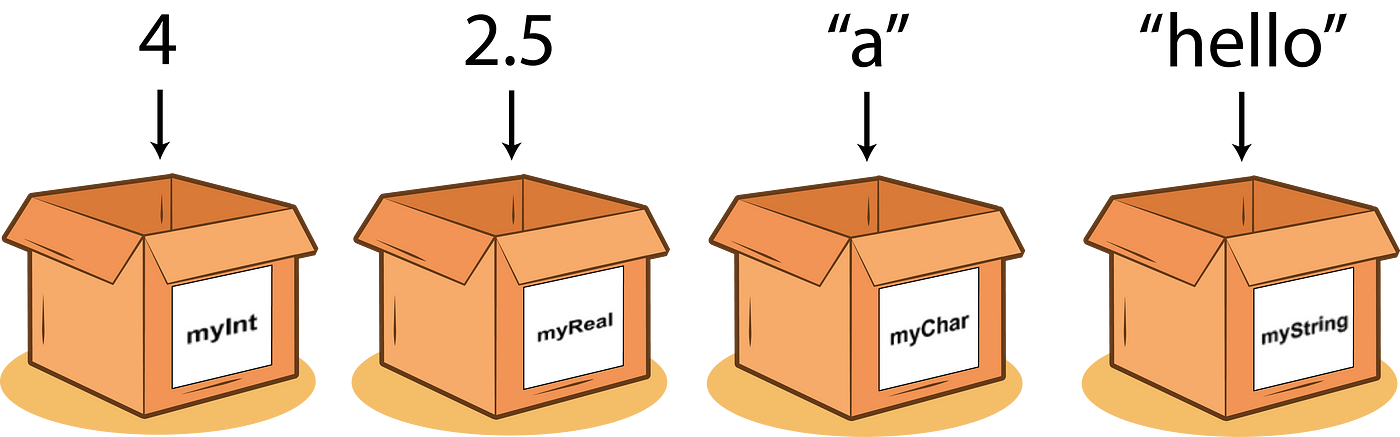
\includegraphics{images/variable.png}

\begin{Shaded}
\begin{Highlighting}[]
\CommentTok{\# Step 1: Define a variable and store the DNA sequence}

\NormalTok{gene\_sequence }\OtherTok{=} \StringTok{"ATCGAGCTAGCTGCTAGCTAGCTAGCT"}

\CommentTok{\# Step 2: Print the stored DNA sequence}

\FunctionTok{print}\NormalTok{(gene\_sequence)}
\end{Highlighting}
\end{Shaded}

\begin{verbatim}
## [1] "ATCGAGCTAGCTGCTAGCTAGCTAGCT"
\end{verbatim}

For instance, consider a situation where you're working with gene sequences. You can use a variable like `gene\_sequence' to store a particular gene's sequence. Later, you can access this stored sequence, manipulate it, or compare it with other sequences as needed in your computational biology tasks.

\hypertarget{data-types}{%
\subsection{Data Types}\label{data-types}}

In programming, similar to the real world, we come across various data types that help us to structure and understand information. These data types include numbers, which could be whole numbers or numbers with decimal points; text, often referred to as strings in programming terms; booleans, representing True or False values; and lists, which are utilized to hold collections of items.

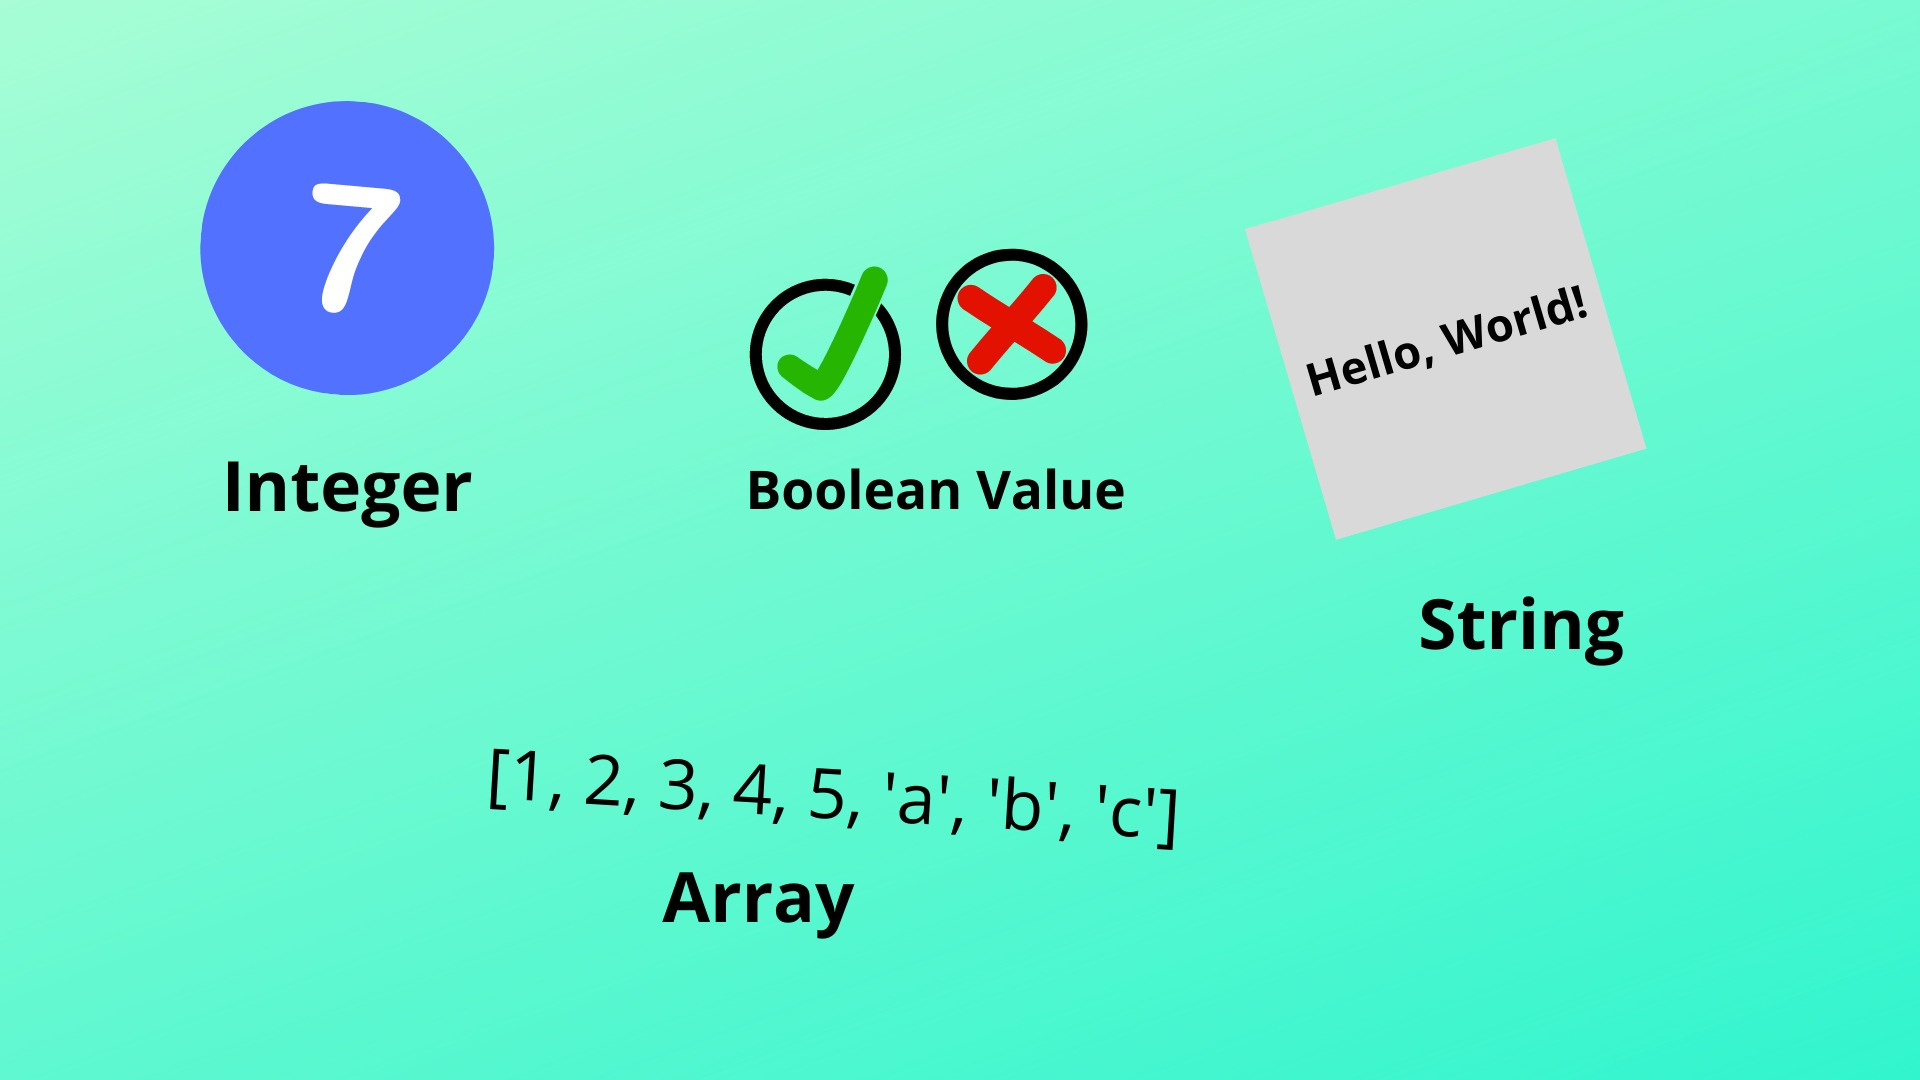
\includegraphics{images/datatype.jpeg}

Each of these data types serve a unique purpose and are used in different contexts, playing an integral role in how we write and interpret code.

\begin{itemize}
\item
  Numbers: In programming, numbers can be whole or decimal. They represent measurements or quantities in computational biology, like DNA length or chemical concentration.
\item
  Text (Strings): Strings are sequences of characters, used for gene names, DNA sequences, or any textual information in computational biology.
\item
  Lists/Arrays: Lists group items together, useful in handling multiple genes, proteins, or biological elements. They can store different gene names or DNA sequences.
\item
  Booleans: Booleans represent true or false values and are used to express conditions or decisions based on a yes/no scenario, like determining if a specific gene is present.
\end{itemize}

Understanding data types is crucial because it helps you work with biological data accurately and efficiently. When you're coding in computational biology, knowing whether you're dealing with numbers, text, or lists allows you to use the right tools and operations for each type of data.

For instance, if you need to perform calculations on gene lengths (numbers), you'll use mathematical operations. If you want to search for a specific gene name (text), you'll use string manipulation techniques. And when you're handling multiple genes (lists), you'll employ list-related functions to process them effectively.

\hypertarget{expressions}{%
\subsection{Expressions}\label{expressions}}

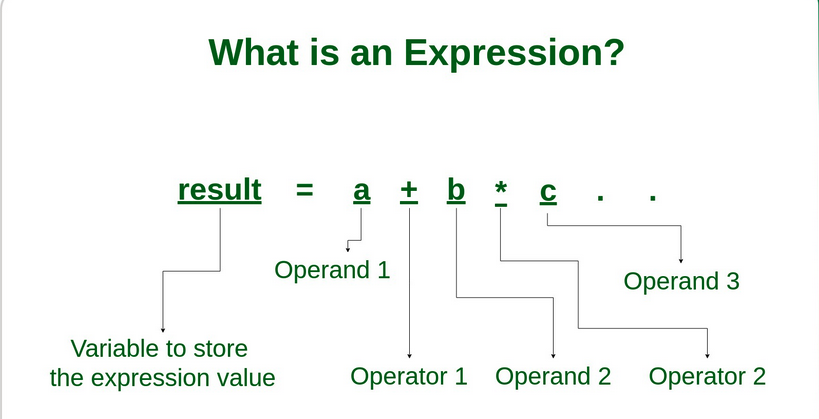
\includegraphics{images/expression.png}

In the world of programming, expressions are like simple puzzles or equations that you can use to do things with data. These expressions are created by putting together a few essential elements:

\begin{itemize}
\item
  Values: Think of these as numbers, like 2 or 3, that you want to work with. In computational biology, these could be things like the length of a gene or the number of amino acids in a protein.
\item
  Variables: These are like labeled containers where you can store information. For example, you might have a variable called `gene\_length' that holds the length of a specific gene sequence.
\item
  Operators: Operators are special symbols like +, -, *, or / that you use to perform operations on values and variables. They tell the computer what kind of action to take.
\end{itemize}

Now, let's dive into some beginner-level examples in computational biology:

\hypertarget{example-finding-the-average-number-of-bases-appearances-in-a-set-of-dna-strings}{%
\subsection{Example: Finding the average number of bases appearances in a set of DNA strings}\label{example-finding-the-average-number-of-bases-appearances-in-a-set-of-dna-strings}}

Let's suppose we want to calculate the average number of bases in a DNA string. Let's assume we already processed the DNA string and we know the counts for each one.

Given counts of each base:

\begin{Shaded}
\begin{Highlighting}[]
\NormalTok{count\_A }\OtherTok{=} \DecValTok{120}

\NormalTok{count\_T }\OtherTok{=} \DecValTok{90}

\NormalTok{count\_C }\OtherTok{=} \DecValTok{80}

\NormalTok{count\_G }\OtherTok{=} \DecValTok{110}
\end{Highlighting}
\end{Shaded}

Calculate the total number of bases

\begin{Shaded}
\begin{Highlighting}[]
\NormalTok{total\_bases }\OtherTok{=}\NormalTok{ count\_A }\SpecialCharTok{+}\NormalTok{ count\_T }\SpecialCharTok{+}\NormalTok{ count\_C }\SpecialCharTok{+}\NormalTok{ count\_G}
\end{Highlighting}
\end{Shaded}

Calculate the average number of bases

\begin{Shaded}
\begin{Highlighting}[]
\NormalTok{average\_bases }\OtherTok{=}\NormalTok{ total\_bases }\SpecialCharTok{/} \DecValTok{4}
\end{Highlighting}
\end{Shaded}

Print the result

\begin{Shaded}
\begin{Highlighting}[]
\FunctionTok{print}\NormalTok{(average\_bases) }
\end{Highlighting}
\end{Shaded}

\begin{verbatim}
## [1] 100
\end{verbatim}

In this code:

\begin{enumerate}
\def\labelenumi{\arabic{enumi}.}
\item
  We start by declaring the counts of each base using variables (number\_a, number\_t, number\_c, number\_g).
\item
  We calculate the total number of bases by summing up the counts.
\item
  Then, we compute the average number of bases by dividing the total by the number of different bases (4 in this case, representing A, T, C, and G).
\item
  Finally, we print the result, which gives us the average number of bases in the DNA string.
\end{enumerate}

\hypertarget{getting-started-with-r-and-rstudio}{%
\chapter{Getting started with R and RStudio}\label{getting-started-with-r-and-rstudio}}

\hypertarget{what-is-r-and-why-is-it-used-in-biology}{%
\section{What is R and why is it used in Biology?}\label{what-is-r-and-why-is-it-used-in-biology}}

In this lesson, we'll dive into the world of R, a powerful programming language and environment used extensively in the field of biology for data analysis and visualization. We'll explore what R is, why it's so useful, and how it can be a valuable tool for biologists.

\hypertarget{what-is-r}{%
\section{What is R?}\label{what-is-r}}

R is a free and open-source statistical programming language specialized for statistical analysis and data visualization. R can supercharge your data analysis and enable you to go beyond the Excel spreadsheet.

\hypertarget{why-is-r-used-in-biology}{%
\section{Why is R Used in Biology?}\label{why-is-r-used-in-biology}}

Biologists use R for a variety of reasons:

\begin{itemize}
\item
  Data Analysis: R provides a wide range of tools and packages for data analysis, making it easier to handle and analyze complex biological datasets. Whether you're studying gene expression, population genetics, or ecological data, R can help you make sense of your data. You can take advantage of a lot of ready-to-use Bioconductor packages for almost any data type in biology. We will learn several essential bioconductor packages in the future sections.
\item
  Statistics: In biology, statistical analysis is crucial for drawing meaningful conclusions from experiments and observations. R offers an extensive collection of statistical functions and libraries, allowing biologists to perform advanced statistical tests and modeling.
\item
  Data Visualization: R excels at creating stunning visualizations of biological data. You can generate graphs, charts, and plots to visualize trends, relationships, and patterns in your data. Visualization is essential for communicating your findings effectively. You can make publication-ready figures with packages such as ggplot2 which we will cover in depth too.
\item
  Reproducibility: R promotes reproducibility in scientific research. You can write scripts or programs to automate your analyses, ensuring that others can replicate your work and verify your results. Tools such as Rmarkdown make the analysis reproducible in Rstudio or Jupyter Notebook.
\item
  Community Support: R has a vibrant and active user community, which means you'll find plenty of resources, tutorials, and forums where you can seek help and share your knowledge. You can visit helpful communities such as the Posit community and Bioconductor support site.
\item
  Integration: R can be integrated with other tools and languages, such as Python and SQL, making it flexible for various research needs.
\end{itemize}

In conclusion, R is a versatile and essential tool for biologists. It empowers researchers to handle, analyze, and visualize data effectively, leading to a deeper understanding of biological phenomena.

\begin{quote}
``Like learning anything, it takes effort to master R. However, if you take the effort to learn the basics and relevant bioinformatics packages, you can conduct your analysis 100 times faster than the point-and-click tools. The added benefit is that you can make your analysis more reproducible.''-- Tommy
\end{quote}

\hypertarget{introduction-to-r-studio}{%
\section{Introduction to R-Studio}\label{introduction-to-r-studio}}

In this chapter, we will introduce you to RStudio, a powerful integrated development environment (IDE) for the R programming language. RStudio provides a user-friendly interface for writing, running, and managing R code. We will explore the various panes, functions, and features of RStudio to help you get started on your journey with R programming.

\hypertarget{introduction-to-r-for-biologists}{%
\chapter{Introduction to R for biologists}\label{introduction-to-r-for-biologists}}

\hypertarget{basic-data-types-in-r}{%
\section{Basic Data Types in R}\label{basic-data-types-in-r}}

\hypertarget{before-starting}{%
\subsection{Before Starting}\label{before-starting}}

When you're working with R, it's crucial to name your variables properly. Here are some simple rules to follow:

\begin{enumerate}
\def\labelenumi{\arabic{enumi}.}
\item
  Allowed Characters: Variable names can include letters, numbers, underscores (\_), and periods (.).
\item
  Starting Characters: A variable name must start with a letter or a period. It can't start with a number.
\item
  Case Sensitivity: R treats variable names as case-sensitive. For example, myvar is different from MyVar.
\item
  Dots in Names: While dots are allowed in variable names, it's best to avoid them except at the beginning.
\item
  Avoiding Conflicts: Don't use names that match existing functions in R, like mean or c.
\end{enumerate}

\hypertarget{examples}{%
\subsubsection{Examples:}\label{examples}}

Valid:

\begin{itemize}
\item
  myvar
\item
  my.var
\item
  var1
\item
  var\_1
\end{itemize}

Invalid:

\begin{itemize}
\item
  1var (can't start with a number)
\item
  \emph{temp (can't start with a })
\item
  c (matches existing function)
\item
  my-var (hyphens aren't allowed)
\item
  my var (spaces aren't allowed)
\end{itemize}

\hypertarget{tips-for-naming}{%
\subsubsection{Tips for Naming:}\label{tips-for-naming}}

\begin{itemize}
\item
  Meaningful Names: Choose descriptive names like patient\_data instead of generic ones like x, y, or z.
\item
  Short and Clear: Keep your names short but make sure they clearly represent what the variable contains.
\item
  Naming Style: You can use camelCase or underscores\_between\_words for multi-word names. Make sure to stick to one style and be consistent.
\end{itemize}

Case Consistency: Decide whether you want all lowercase names or CapWords (also known as PascalCase), and stick to it throughout your code.

By following these naming conventions, your code will be easier to understand, and you'll avoid unexpected errors. Consistency is key when naming variables across your R scripts.

In R, data can be classified into several fundamental types, each serving specific purposes in data analysis and manipulation. Understanding these data types is crucial for effective data handling. Let's explore the primary data types in R:

\hypertarget{numeric}{%
\subsection{1. Numeric}\label{numeric}}

Numeric data represents continuous numerical values. These can be integers or real numbers (floating-point). Numeric data is used for mathematical calculations and statistical analysis.

Example:

\begin{Shaded}
\begin{Highlighting}[]
\CommentTok{\# Numeric data}
\NormalTok{age }\OtherTok{\textless{}{-}} \DecValTok{28}
\NormalTok{height }\OtherTok{\textless{}{-}} \FloatTok{1.75}
\end{Highlighting}
\end{Shaded}

The \texttt{\textless{}-} operator and the \texttt{=} operator in R are both used for assignment but have some key differences.

The \texttt{\textless{}-} operator is the standard assignment operator in R. It assigns values to objects.

\begin{itemize}
\item
  The arrow can be read as ``gets''. So age gets the value of 28.
\item
  All R objects should be created using the \texttt{\textless{}-} operator.
\end{itemize}

The \texttt{=} Operator can also be used for assignments.

\begin{Shaded}
\begin{Highlighting}[]
\NormalTok{age }\OtherTok{=} \DecValTok{28}
\end{Highlighting}
\end{Shaded}

\begin{itemize}
\item
  This also assigns 28 to age.
\item
  The \texttt{=} should be read as ``is equal to''. This is mainly used to specify function arguments.
\end{itemize}

So in a function call like:

\begin{Shaded}
\begin{Highlighting}[]
\FunctionTok{plot}\NormalTok{(}\AttributeTok{x =}\NormalTok{ mydata)}
\end{Highlighting}
\end{Shaded}

We are specifying that the x argument is equal to mydata.

In summary, \texttt{\textless{}-} is the operator you should use when creating R objects, while
\texttt{=} is reserved for function arguments. For assignments, both \texttt{\textless{}-} and \texttt{=} can be used.
If you want to read more differences, take a look at \url{https://stat.ethz.ch/R-manual/R-patched/library/base/html/assignOps.html}.

\hypertarget{character-string}{%
\subsection{2. Character (String)}\label{character-string}}

Character data represents text or strings of characters. You use character data for storing and manipulating text-based information, such as names, descriptions, and labels.

Example:

\begin{Shaded}
\begin{Highlighting}[]
\CommentTok{\# Character data}
\NormalTok{name }\OtherTok{\textless{}{-}} \StringTok{"John Doe"}
\NormalTok{city }\OtherTok{\textless{}{-}} \StringTok{"New York"}
\end{Highlighting}
\end{Shaded}

\hypertarget{integer}{%
\subsection{3. Integer}\label{integer}}

Integer data represents whole numbers. Unlike numeric data, which includes decimal points, integer data includes only whole numbers. It's commonly used when dealing with counts or discrete quantities.

Example:

\begin{Shaded}
\begin{Highlighting}[]
\CommentTok{\# Integer data}
\NormalTok{count }\OtherTok{\textless{}{-}} \DecValTok{10}
\NormalTok{students }\OtherTok{\textless{}{-}} \DecValTok{42}
\end{Highlighting}
\end{Shaded}

\hypertarget{logical-boolean}{%
\subsection{4. Logical (Boolean)}\label{logical-boolean}}

Logical data consists of two possible values: \texttt{TRUE} or \texttt{FALSE}. These values are used for binary decisions, conditions, and logical operations.

Example:

\begin{Shaded}
\begin{Highlighting}[]
\CommentTok{\# Logical data}
\NormalTok{is\_student }\OtherTok{\textless{}{-}} \ConstantTok{TRUE}
\NormalTok{has\_permission }\OtherTok{\textless{}{-}} \ConstantTok{FALSE}
\end{Highlighting}
\end{Shaded}

\hypertarget{factor}{%
\subsection{5. Factor}\label{factor}}

Factor data represents categorical variables with predefined levels or categories. Factors are used when you have data that can be divided into distinct categories, such as ``High,'' ``Medium,'' and ``Low.''

Example:

\begin{Shaded}
\begin{Highlighting}[]
\CommentTok{\# Factor data}
\NormalTok{grade }\OtherTok{\textless{}{-}} \FunctionTok{factor}\NormalTok{(}\FunctionTok{c}\NormalTok{(}\StringTok{"A"}\NormalTok{, }\StringTok{"B"}\NormalTok{, }\StringTok{"C"}\NormalTok{, }\StringTok{"B"}\NormalTok{, }\StringTok{"A"}\NormalTok{))}
\end{Highlighting}
\end{Shaded}

\hypertarget{date-and-time}{%
\subsection{6. Date and Time}\label{date-and-time}}

Date and time data types are used for representing dates, times, or both. These data types are crucial when dealing with time series data or conducting temporal analysis.

Example:

\begin{Shaded}
\begin{Highlighting}[]
\CommentTok{\# Date and time data}
\NormalTok{birth\_date }\OtherTok{\textless{}{-}} \FunctionTok{as.Date}\NormalTok{(}\StringTok{"1990{-}05{-}15"}\NormalTok{)}
\NormalTok{timestamp }\OtherTok{\textless{}{-}} \FunctionTok{as.POSIXct}\NormalTok{(}\StringTok{"2023{-}01{-}09 14:30:00"}\NormalTok{)}
\end{Highlighting}
\end{Shaded}

\hypertarget{complex}{%
\subsection{7. Complex}\label{complex}}

Complex data types represent complex numbers, which have both real and imaginary parts. Complex numbers are used in advanced mathematical and engineering applications.

Example:

\begin{Shaded}
\begin{Highlighting}[]
\CommentTok{\# Complex data}
\NormalTok{z }\OtherTok{\textless{}{-}} \DecValTok{3} \SpecialCharTok{+}\NormalTok{ 2i}
\end{Highlighting}
\end{Shaded}

\hypertarget{missing-values-na}{%
\subsection{8. Missing Values (NA)}\label{missing-values-na}}

In R, missing values are represented as NA. These values indicate the absence of data or an undefined value. Handling missing data is essential in data analysis.

Example:

\begin{Shaded}
\begin{Highlighting}[]
\CommentTok{\# Missing value}
\NormalTok{missing\_data }\OtherTok{\textless{}{-}} \ConstantTok{NA}
\end{Highlighting}
\end{Shaded}

Understanding these data types and their characteristics is fundamental to effective data manipulation and analysis in R. Different operations and functions may behave differently depending on the data type, so being familiar with these types will help you work with data effectively.

\hypertarget{the-key-concept-of-r-vectors}{%
\section{The key concept of R: Vectors}\label{the-key-concept-of-r-vectors}}

In the world of R, vectors are the building blocks of data. In fact, everything in R is a vector. Whether you're dealing with numbers or characters, R treats them all as vectors, which are simply collections of these elements. There is no concept of a scalar in R; even a single value is considered a one-element vector. To create a vector, you'll use the c function, which stands for ``combine'' or ``concatenate.''

\hypertarget{creating-numeric-and-character-vectors}{%
\subsection{Creating Numeric and Character Vectors}\label{creating-numeric-and-character-vectors}}

Let's dive right in with examples:

\begin{Shaded}
\begin{Highlighting}[]
\CommentTok{\# A numeric vector}
\FunctionTok{c}\NormalTok{(}\DecValTok{1}\NormalTok{, }\DecValTok{2}\NormalTok{, }\DecValTok{3}\NormalTok{)}
\end{Highlighting}
\end{Shaded}

\begin{verbatim}
## [1] 1 2 3
\end{verbatim}

\begin{Shaded}
\begin{Highlighting}[]
\CommentTok{\# Output: [1] 1 2 3}

\CommentTok{\# A character vector}
\FunctionTok{c}\NormalTok{(}\StringTok{"A"}\NormalTok{, }\StringTok{"T"}\NormalTok{, }\StringTok{"C"}\NormalTok{, }\StringTok{"G"}\NormalTok{)}
\end{Highlighting}
\end{Shaded}

\begin{verbatim}
## [1] "A" "T" "C" "G"
\end{verbatim}

\begin{Shaded}
\begin{Highlighting}[]
\CommentTok{\# Output: [1] "A" "T" "C" "G"}
\end{Highlighting}
\end{Shaded}

Notice how \texttt{c()} is used to combine values into vectors. Even a single element, such as ``A'', is a vector in R. Similarly, numeric values like 5 are considered one-element vectors.

\hypertarget{saving-vectors-to-variables}{%
\subsection{Saving Vectors to Variables}\label{saving-vectors-to-variables}}

Now, let's save these vectors into variables with meaningful names:

\begin{Shaded}
\begin{Highlighting}[]
\NormalTok{number\_vec }\OtherTok{\textless{}{-}} \FunctionTok{c}\NormalTok{(}\DecValTok{1}\NormalTok{, }\DecValTok{2}\NormalTok{, }\DecValTok{3}\NormalTok{)}
\NormalTok{dna\_base }\OtherTok{\textless{}{-}} \FunctionTok{c}\NormalTok{(}\StringTok{"A"}\NormalTok{, }\StringTok{"T"}\NormalTok{, }\StringTok{"C"}\NormalTok{, }\StringTok{"G"}\NormalTok{) }
\NormalTok{gene\_ids }\OtherTok{\textless{}{-}} \FunctionTok{c}\NormalTok{(}\StringTok{"PAX6"}\NormalTok{, }\StringTok{"TP53"}\NormalTok{, }\StringTok{"MYC"}\NormalTok{)}
\end{Highlighting}
\end{Shaded}

Remember, it's good practice to use informative variable names. Variable names cannot start with a number, so opt for names like \texttt{number\_vec} and \texttt{dna\_base}.

\hypertarget{vectorized-calculations}{%
\subsection{Vectorized Calculations}\label{vectorized-calculations}}

One of the powerful features of R is vectorization, where operations are automatically applied element-wise to vectors. For example:

\begin{Shaded}
\begin{Highlighting}[]
\NormalTok{number\_vec }\SpecialCharTok{+} \DecValTok{1} 
\end{Highlighting}
\end{Shaded}

\begin{verbatim}
## [1] 2 3 4
\end{verbatim}

Here, we've added 1 to each element of \texttt{number\_vec}. This vectorized behavior simplifies many calculations.

\hypertarget{understanding-indexing}{%
\subsubsection{Understanding Indexing}\label{understanding-indexing}}

You may have noticed the \texttt{{[}1{]}} that appears in the output. In R, it's called an index, and it indicates the position of each element in the result. For instance:

\begin{Shaded}
\begin{Highlighting}[]
\NormalTok{x }\OtherTok{\textless{}{-}} \DecValTok{1}\SpecialCharTok{:}\DecValTok{100}
\NormalTok{x}
\end{Highlighting}
\end{Shaded}

\begin{verbatim}
##   [1]   1   2   3   4   5   6   7   8   9  10  11  12  13  14  15  16  17  18
##  [19]  19  20  21  22  23  24  25  26  27  28  29  30  31  32  33  34  35  36
##  [37]  37  38  39  40  41  42  43  44  45  46  47  48  49  50  51  52  53  54
##  [55]  55  56  57  58  59  60  61  62  63  64  65  66  67  68  69  70  71  72
##  [73]  73  74  75  76  77  78  79  80  81  82  83  84  85  86  87  88  89  90
##  [91]  91  92  93  94  95  96  97  98  99 100
\end{verbatim}

In this case, \texttt{{[}1{]}} denotes the first position of each element. Understanding indexing helps when working with large datasets.

\hypertarget{performing-vectorized-calculations}{%
\subsection{Performing Vectorized Calculations}\label{performing-vectorized-calculations}}

You can perform various calculations on vectors in R:

\begin{Shaded}
\begin{Highlighting}[]
\NormalTok{number\_vec }\SpecialCharTok{*} \DecValTok{2}
\end{Highlighting}
\end{Shaded}

\begin{verbatim}
## [1] 2 4 6
\end{verbatim}

\begin{Shaded}
\begin{Highlighting}[]
\CommentTok{\# Output: [1] 2 4 6}

\NormalTok{number\_vec }\SpecialCharTok{/} \DecValTok{2}
\end{Highlighting}
\end{Shaded}

\begin{verbatim}
## [1] 0.5 1.0 1.5
\end{verbatim}

\begin{Shaded}
\begin{Highlighting}[]
\CommentTok{\# Output: [1] 0.5 1.0 1.5}
\end{Highlighting}
\end{Shaded}

Remember, all these calculations are vectorized, making R a powerful tool for data manipulation.

\hypertarget{operations-with-character-vectors}{%
\subsection{Operations with character vectors}\label{operations-with-character-vectors}}

Character vectors in R offer a wide range of operations for text manipulation and analysis. Let's explore some of the essential operations:

\hypertarget{concatenation}{%
\subsubsection{Concatenation}\label{concatenation}}

You can combine character vectors using the c function:

\begin{Shaded}
\begin{Highlighting}[]
\NormalTok{new\_bases }\OtherTok{\textless{}{-}} \FunctionTok{c}\NormalTok{(dna\_base, }\StringTok{"N"}\NormalTok{)}
\NormalTok{new\_bases}
\end{Highlighting}
\end{Shaded}

\begin{verbatim}
## [1] "A" "T" "C" "G" "N"
\end{verbatim}

This operation is useful for extending or combining character vectors.

\hypertarget{changing-case}{%
\subsubsection{Changing Case}\label{changing-case}}

Transforming the case of characters is straightforward in R. You can convert characters to uppercase or lowercase:

\begin{Shaded}
\begin{Highlighting}[]
\FunctionTok{toupper}\NormalTok{(dna\_base)}
\end{Highlighting}
\end{Shaded}

\begin{verbatim}
## [1] "A" "T" "C" "G"
\end{verbatim}

\begin{Shaded}
\begin{Highlighting}[]
\FunctionTok{tolower}\NormalTok{(dna\_base)}
\end{Highlighting}
\end{Shaded}

\begin{verbatim}
## [1] "a" "t" "c" "g"
\end{verbatim}

This is handy when you need consistent formatting.

\hypertarget{logical-vectors}{%
\subsection{Logical Vectors}\label{logical-vectors}}

Character vectors also allow for logical operations, which can be incredibly powerful

\hypertarget{finding-matches}{%
\subsubsection{Finding Matches}\label{finding-matches}}

To check which elements in a character vector meet certain criteria, use the \%in\% operator:

\begin{Shaded}
\begin{Highlighting}[]
\NormalTok{dna\_base }\SpecialCharTok{\%in\%} \FunctionTok{c}\NormalTok{(}\StringTok{"A"}\NormalTok{, }\StringTok{"C"}\NormalTok{, }\StringTok{"T"}\NormalTok{)}
\end{Highlighting}
\end{Shaded}

\begin{verbatim}
## [1]  TRUE  TRUE  TRUE FALSE
\end{verbatim}

This produces a logical vector where \texttt{TRUE} indicates a match. This is because the vector dna\_base contains \texttt{A}, \texttt{T}, \texttt{C}, \texttt{G} and \texttt{G} does not match any element in the vector created by \texttt{c("A",\ "C",\ "T")}.

\hypertarget{saving-a-logical-vector}{%
\subsubsection{Saving a Logical Vector}\label{saving-a-logical-vector}}

Save the resulting logical vector to a new variable for future use:

\begin{Shaded}
\begin{Highlighting}[]
\NormalTok{logical\_vec }\OtherTok{\textless{}{-}}\NormalTok{ dna\_base }\SpecialCharTok{\%in\%} \FunctionTok{c}\NormalTok{(}\StringTok{"A"}\NormalTok{, }\StringTok{"C"}\NormalTok{, }\StringTok{"T"}\NormalTok{)}
\NormalTok{logical\_vec}
\end{Highlighting}
\end{Shaded}

\begin{verbatim}
## [1]  TRUE  TRUE  TRUE FALSE
\end{verbatim}

The length of the logical vector matches the original character vector.

\hypertarget{negating-a-logical-vector}{%
\subsubsection{Negating a Logical Vector}\label{negating-a-logical-vector}}

You can negate a logical vector using the \texttt{!} operator:

\begin{Shaded}
\begin{Highlighting}[]
\SpecialCharTok{!}\NormalTok{logical\_vec}
\end{Highlighting}
\end{Shaded}

\begin{verbatim}
## [1] FALSE FALSE FALSE  TRUE
\end{verbatim}

Now, \texttt{TRUE} represents elements that do not match the criteria.

\hypertarget{subsetting-with-logical-vectors}{%
\subsubsection{Subsetting with Logical Vectors}\label{subsetting-with-logical-vectors}}

Using a logical vector for subsetting another vector is a common operation. It allows you to filter and extract specific elements:

\begin{Shaded}
\begin{Highlighting}[]
\CommentTok{\# Subsetting elements that meet the criteria}
\NormalTok{dna\_base[logical\_vec]}
\end{Highlighting}
\end{Shaded}

\begin{verbatim}
## [1] "A" "T" "C"
\end{verbatim}

\begin{Shaded}
\begin{Highlighting}[]
\CommentTok{\# Subsetting elements that do not meet the criteria}
\NormalTok{dna\_base[}\SpecialCharTok{!}\NormalTok{logical\_vec]}
\end{Highlighting}
\end{Shaded}

\begin{verbatim}
## [1] "G"
\end{verbatim}

This powerful technique helps you extract and manipulate data efficiently based on specified conditions.

\hypertarget{conclusion}{%
\subsection{Conclusion}\label{conclusion}}

You've learned the fundamental operations that can be performed on both numeric and character vectors. These essential skills will serve as a strong foundation as you delve deeper into the world of data analysis and manipulation using R.

Remember that vectors are the building blocks of R, and they are used extensively in various data analysis tasks. Whether you're combining elements, changing case, or using logical operations to filter and extract data, you have now gained valuable insights into how vectors can be harnessed to accomplish your data analysis goals.

As you continue your journey in R programming, you'll encounter more complex data structures and operations, but the understanding of vectors will remain a cornerstone of your proficiency.

\hypertarget{subsetting-and-indexing}{%
\section{Subsetting and Indexing}\label{subsetting-and-indexing}}

In this guide, we will explain one of the fundamental concepts for dealing with vectors: indexing and slicing. Understanding how R handles these operations is crucial as it differs from some other programming languages, like Python.

\hypertarget{indexing-in-r}{%
\subsection{Indexing in R}\label{indexing-in-r}}

In R, unlike Python where indexing starts at 0, it begins at 1. This means that the first element in a sequence is located at position 1, the second at position 2, and so on. Let's dive into some practical examples to illustrate this concept.

\begin{Shaded}
\begin{Highlighting}[]
\CommentTok{\# Let\textquotesingle{}s create a vector of DNA bases}
\NormalTok{dna\_base }\OtherTok{\textless{}{-}} \FunctionTok{c}\NormalTok{(}\StringTok{"A"}\NormalTok{, }\StringTok{"T"}\NormalTok{, }\StringTok{"C"}\NormalTok{, }\StringTok{"G"}\NormalTok{)}

\CommentTok{\# Accessing the second element (T) using indexing}
\NormalTok{dna\_base[}\DecValTok{2}\NormalTok{]}
\end{Highlighting}
\end{Shaded}

\begin{verbatim}
## [1] "T"
\end{verbatim}

\begin{Shaded}
\begin{Highlighting}[]
\CommentTok{\# second and fourth element}
\NormalTok{dna\_base[}\FunctionTok{c}\NormalTok{(}\DecValTok{2}\NormalTok{,}\DecValTok{4}\NormalTok{)]}
\end{Highlighting}
\end{Shaded}

\begin{verbatim}
## [1] "T" "G"
\end{verbatim}

Here, we use square brackets \texttt{{[}\ {]}} to access elements by their position in the dna\_base vector. So, \texttt{dna\_base{[}2{]}} returns the second element, which is ``T''.

\hypertarget{slicing-in-r}{%
\subsection{Slicing in R}\label{slicing-in-r}}

Slicing in R allows you to extract a chunk of elements from a vector or sequence. You can specify the start and end positions within the square brackets to define the slice.

\begin{Shaded}
\begin{Highlighting}[]
\CommentTok{\# Slicing the first two elements (A and T) from the dna\_base vector}
\NormalTok{dna\_base[}\DecValTok{1}\SpecialCharTok{:}\DecValTok{2}\NormalTok{]}
\end{Highlighting}
\end{Shaded}

\begin{verbatim}
## [1] "A" "T"
\end{verbatim}

In this example, \texttt{dna\_base{[}1:2{]}} retrieves elements from position 1 to 2, giving us ``A'' and ``T''.

\hypertarget{negative-indexing}{%
\subsection{Negative Indexing}\label{negative-indexing}}

R also allows negative indexing to remove that element at that position:

\begin{Shaded}
\begin{Highlighting}[]
\CommentTok{\# remove first element by negative indexing}
\NormalTok{remove\_first\_element }\OtherTok{\textless{}{-}}\NormalTok{ dna\_base[}\SpecialCharTok{{-}}\DecValTok{1}\NormalTok{]}
\end{Highlighting}
\end{Shaded}

\begin{Shaded}
\begin{Highlighting}[]
\CommentTok{\# remove second and fourth}
\NormalTok{dna\_base[}\SpecialCharTok{{-}}\FunctionTok{c}\NormalTok{(}\DecValTok{2}\NormalTok{,}\DecValTok{4}\NormalTok{)]}
\end{Highlighting}
\end{Shaded}

\begin{verbatim}
## [1] "A" "C"
\end{verbatim}

\begin{Shaded}
\begin{Highlighting}[]
\CommentTok{\# Output: [1] "A" "C"}
\end{Highlighting}
\end{Shaded}

\hypertarget{conclusion-1}{%
\subsection{Conclusion}\label{conclusion-1}}

Remember that R starts indexing at 1, not 0, and you can use square brackets \texttt{{[}\ {]}} to access elements and slices within vectors and sequences. This is essential for working with data and performing various operations in R.

\hypertarget{understanding-and-manipulating-matrices}{%
\section{Understanding and Manipulating Matrices}\label{understanding-and-manipulating-matrices}}

Matrices are essential for organizing and processing data, especially when dealing with gene expression data from technologies like RNA sequencing (RNAseq). In this tutorial, we will explore how to create, manipulate, and extract information from matrices using the R programming language. We will cover topics ranging from basic matrix operations to more advanced tasks like normalization for RNAseq data analysis.

\hypertarget{creating-a-matrix}{%
\subsection{Creating a Matrix}\label{creating-a-matrix}}

To create a matrix in R, you can use the matrix() function. A matrix is essentially a 2-dimensional table for storing numerical data. Let's start by creating a simple matrix:

\begin{Shaded}
\begin{Highlighting}[]
\NormalTok{expression\_mat }\OtherTok{\textless{}{-}} \FunctionTok{matrix}\NormalTok{(}\DecValTok{1}\SpecialCharTok{:}\DecValTok{12}\NormalTok{, }\AttributeTok{nrow =} \DecValTok{3}\NormalTok{, }\AttributeTok{ncol =} \DecValTok{4}\NormalTok{)}
\NormalTok{expression\_mat}
\end{Highlighting}
\end{Shaded}

\begin{verbatim}
##      [,1] [,2] [,3] [,4]
## [1,]    1    4    7   10
## [2,]    2    5    8   11
## [3,]    3    6    9   12
\end{verbatim}

Here, \texttt{expression\_mat} is a dummy gene expression matrix with 3 rows (genes) and 4 columns (samples), where the entries represent counts for each gene in each sample.

\hypertarget{adding-row-and-column-names}{%
\subsection{Adding Row and Column Names}\label{adding-row-and-column-names}}

You can enhance the clarity of your matrix by adding row and column names. This is particularly useful when dealing with real biological data. For example:

\begin{Shaded}
\begin{Highlighting}[]
\FunctionTok{rownames}\NormalTok{(expression\_mat) }\OtherTok{\textless{}{-}} \FunctionTok{c}\NormalTok{(}\StringTok{"gene1"}\NormalTok{, }\StringTok{"gene2"}\NormalTok{, }\StringTok{"gene3"}\NormalTok{)}
\FunctionTok{colnames}\NormalTok{(expression\_mat) }\OtherTok{\textless{}{-}} \FunctionTok{c}\NormalTok{(}\StringTok{"sample1"}\NormalTok{, }\StringTok{"sample2"}\NormalTok{, }\StringTok{"sample3"}\NormalTok{, }\StringTok{"sample4"}\NormalTok{)}
\NormalTok{expression\_mat}
\end{Highlighting}
\end{Shaded}

\begin{verbatim}
##       sample1 sample2 sample3 sample4
## gene1       1       4       7      10
## gene2       2       5       8      11
## gene3       3       6       9      12
\end{verbatim}

Now, instead of numerical indices, your matrix displays gene and sample names, making it easier to interpret.

\hypertarget{subsetting-a-matrix}{%
\subsection{Subsetting a Matrix}\label{subsetting-a-matrix}}

Subsetting allows you to extract specific rows and columns from a matrix. You can use numerical indices, row/column names, or logical vectors. Remember, R is 1-based. Indices start at 1 while Python starts at 0.

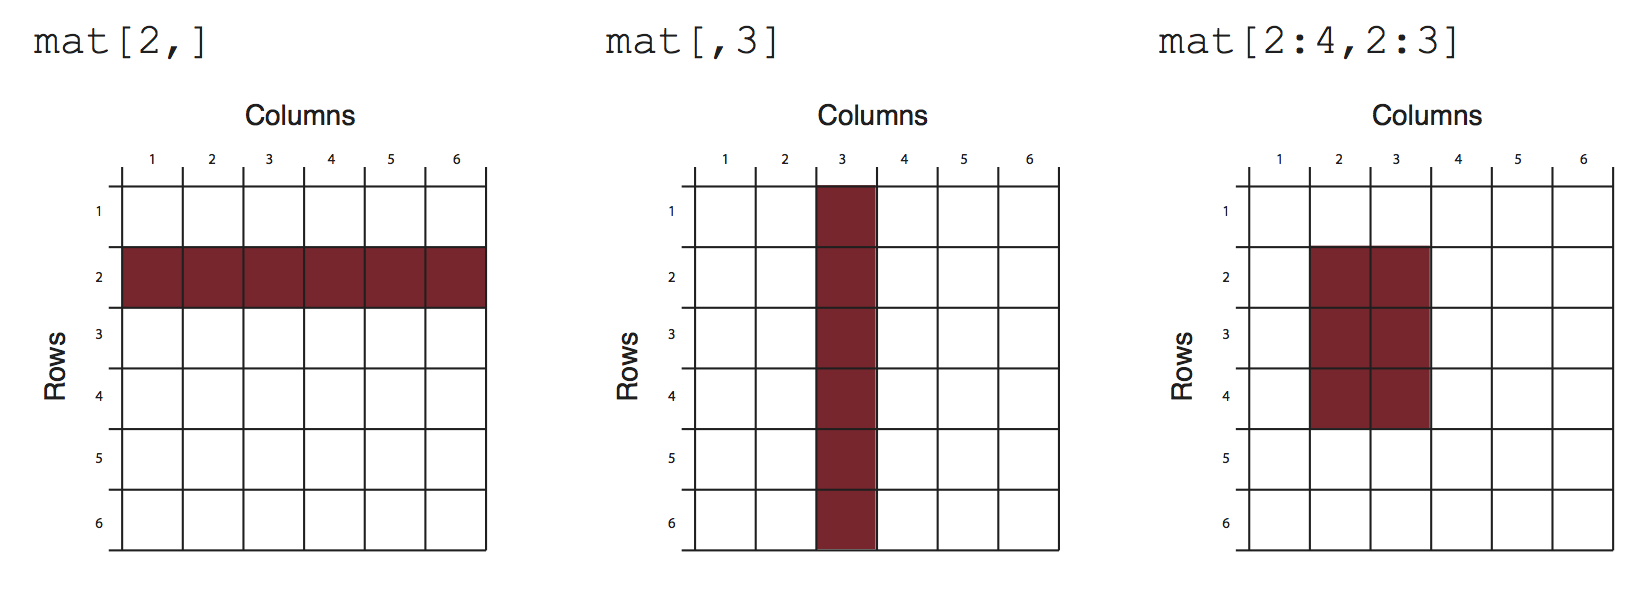
\includegraphics{images/matrix.png}

\hypertarget{subsetting-using-numerical-indices}{%
\subsubsection{Subsetting using numerical indices}\label{subsetting-using-numerical-indices}}

\begin{Shaded}
\begin{Highlighting}[]
\CommentTok{\# Accessing a single element}
\NormalTok{expression\_mat[}\DecValTok{1}\NormalTok{, }\DecValTok{2}\NormalTok{]}
\end{Highlighting}
\end{Shaded}

\begin{verbatim}
## [1] 4
\end{verbatim}

slice a chunk

\begin{Shaded}
\begin{Highlighting}[]
\NormalTok{expression\_mat[}\DecValTok{1}\SpecialCharTok{:}\DecValTok{2}\NormalTok{, }\DecValTok{1}\SpecialCharTok{:}\DecValTok{2}\NormalTok{]}
\end{Highlighting}
\end{Shaded}

\begin{verbatim}
##       sample1 sample2
## gene1       1       4
## gene2       2       5
\end{verbatim}

If you leave either the row index blank or the column index, it will subset all the rows or columns. Subset the first two rows and all columns:

\begin{Shaded}
\begin{Highlighting}[]
\NormalTok{expression\_mat[}\DecValTok{1}\SpecialCharTok{:}\DecValTok{2}\NormalTok{,]}
\end{Highlighting}
\end{Shaded}

\begin{verbatim}
##       sample1 sample2 sample3 sample4
## gene1       1       4       7      10
## gene2       2       5       8      11
\end{verbatim}

Subset the columns 2 and 4 and all rows

\begin{Shaded}
\begin{Highlighting}[]
\NormalTok{expression\_mat[, }\FunctionTok{c}\NormalTok{(}\DecValTok{2}\NormalTok{,}\DecValTok{4}\NormalTok{)]}
\end{Highlighting}
\end{Shaded}

\begin{verbatim}
##       sample2 sample4
## gene1       4      10
## gene2       5      11
## gene3       6      12
\end{verbatim}

\hypertarget{subsetting-using-row-names}{%
\subsubsection{Subsetting using row names}\label{subsetting-using-row-names}}

\begin{Shaded}
\begin{Highlighting}[]
\CommentTok{\# Accessing a specific gene\textquotesingle{}s data}
\NormalTok{expression\_mat[}\StringTok{"gene3"}\NormalTok{, ]}
\end{Highlighting}
\end{Shaded}

\begin{verbatim}
## sample1 sample2 sample3 sample4 
##       3       6       9      12
\end{verbatim}

When only one row or one column is left after subsetting, R returns a vector instead of a matrix. To return a single row or column matrix, add \texttt{drop=FALSE}.

\begin{Shaded}
\begin{Highlighting}[]
\NormalTok{expression\_mat[}\StringTok{"gene3"}\NormalTok{, , drop}\OtherTok{=}\ConstantTok{FALSE}\NormalTok{]}
\end{Highlighting}
\end{Shaded}

\begin{verbatim}
##       sample1 sample2 sample3 sample4
## gene3       3       6       9      12
\end{verbatim}

\hypertarget{subsetting-using-column-names}{%
\subsubsection{Subsetting using column names}\label{subsetting-using-column-names}}

\begin{Shaded}
\begin{Highlighting}[]
\CommentTok{\# Using predefined gene and sample names}
\NormalTok{differential\_genes}\OtherTok{\textless{}{-}} \FunctionTok{c}\NormalTok{(}\StringTok{"gene3"}\NormalTok{, }\StringTok{"gene1"}\NormalTok{)}
\NormalTok{expression\_mat[differential\_genes, }\FunctionTok{c}\NormalTok{(}\StringTok{"sample1"}\NormalTok{, }\StringTok{"sample2"}\NormalTok{)]}
\end{Highlighting}
\end{Shaded}

\begin{verbatim}
##       sample1 sample2
## gene3       3       6
## gene1       1       4
\end{verbatim}

You see how the matrix is subsetted and the row names are ordered as in \texttt{differential\_genes}.

\hypertarget{subsetting-using-logical-vectors}{%
\subsubsection{Subsetting using logical vectors}\label{subsetting-using-logical-vectors}}

We have a matrix called \texttt{expression\_mat} that contains gene expression data, and you want to subset it to include only the rows corresponding to certain ``differential genes.'' Here's how you can do it:

\begin{Shaded}
\begin{Highlighting}[]
\NormalTok{logical\_vec\_genes }\OtherTok{\textless{}{-}} \FunctionTok{rownames}\NormalTok{(expression\_mat) }\SpecialCharTok{\%in\%}\NormalTok{ differential\_genes}
\NormalTok{expression\_mat[logical\_vec\_genes,]}
\end{Highlighting}
\end{Shaded}

\begin{verbatim}
##       sample1 sample2 sample3 sample4
## gene1       1       4       7      10
## gene3       3       6       9      12
\end{verbatim}

\hypertarget{calculations-with-matrices}{%
\subsection{Calculations with Matrices}\label{calculations-with-matrices}}

You can perform various calculations on matrices, such as calculating the sum of counts for each sample (column level) or gene (row level):

\begin{Shaded}
\begin{Highlighting}[]
\FunctionTok{colSums}\NormalTok{(expression\_mat)}
\end{Highlighting}
\end{Shaded}

\begin{verbatim}
## sample1 sample2 sample3 sample4 
##       6      15      24      33
\end{verbatim}

\begin{Shaded}
\begin{Highlighting}[]
\FunctionTok{rowSums}\NormalTok{(expression\_mat)}
\end{Highlighting}
\end{Shaded}

\begin{verbatim}
## gene1 gene2 gene3 
##    22    26    30
\end{verbatim}

\hypertarget{normalization}{%
\subsection{Normalization}\label{normalization}}

Normalization is crucial in RNAseq data analysis to account for differences in sequencing depth and gene length. Two common methods for normalization are RPKM (Reads Per Kilobase per Million) and TPM (Transcripts Per Million). Watch this video to understand better of their differences

\begin{quote}
RPKM (Reads Per Kilobase per Million) and TPM (Transcripts Per Million) are two widely-used methods for normalizing gene expression data in RNAseq, with RPKM considering gene length and total reads per sample and TPM further accounting for differences in sequencing depth between samples.
\end{quote}

Here's how you can normalize a matrix to RPKM and TPM:

\begin{Shaded}
\begin{Highlighting}[]
\CommentTok{\# Gene lengths (in kilobases)}
\NormalTok{gene\_lengths }\OtherTok{\textless{}{-}} \FunctionTok{c}\NormalTok{(}\DecValTok{1000}\NormalTok{, }\DecValTok{2000}\NormalTok{, }\DecValTok{3000}\NormalTok{)}

\CommentTok{\# Normalizing to RPKM}
\NormalTok{rpkm\_normalized }\OtherTok{\textless{}{-}} \FunctionTok{t}\NormalTok{(}\FunctionTok{t}\NormalTok{(expression\_mat)}\SpecialCharTok{/}\FunctionTok{colSums}\NormalTok{(expression\_mat))}\SpecialCharTok{/}\NormalTok{gene\_lengths }\SpecialCharTok{*} \FloatTok{1e6}
\NormalTok{rpkm\_normalized}
\end{Highlighting}
\end{Shaded}

\begin{verbatim}
##        sample1  sample2  sample3  sample4
## gene1 166.6667 266.6667 291.6667 303.0303
## gene2 166.6667 166.6667 166.6667 166.6667
## gene3 166.6667 133.3333 125.0000 121.2121
\end{verbatim}

\begin{Shaded}
\begin{Highlighting}[]
\CommentTok{\# Normalizing to TPM}
\NormalTok{tpm\_normalized }\OtherTok{\textless{}{-}} \FunctionTok{t}\NormalTok{(}\FunctionTok{t}\NormalTok{(expression\_mat}\SpecialCharTok{/}\NormalTok{gene\_lengths)}\SpecialCharTok{/} \FunctionTok{colSums}\NormalTok{((expression\_mat}\SpecialCharTok{/}\NormalTok{gene\_lengths))) }\SpecialCharTok{*} \FloatTok{1e6}

\NormalTok{tpm\_normalized}
\end{Highlighting}
\end{Shaded}

\begin{verbatim}
##        sample1  sample2  sample3  sample4
## gene1 333333.3 470588.2 500000.0 512820.5
## gene2 333333.3 294117.6 285714.3 282051.3
## gene3 333333.3 235294.1 214285.7 205128.2
\end{verbatim}

Note, when you divide a matrix by a vector, the operation is row-wise.

\begin{Shaded}
\begin{Highlighting}[]
\NormalTok{expression\_mat}
\end{Highlighting}
\end{Shaded}

\begin{verbatim}
##       sample1 sample2 sample3 sample4
## gene1       1       4       7      10
## gene2       2       5       8      11
## gene3       3       6       9      12
\end{verbatim}

\begin{Shaded}
\begin{Highlighting}[]
\NormalTok{gene\_lengths}
\end{Highlighting}
\end{Shaded}

\begin{verbatim}
## [1] 1000 2000 3000
\end{verbatim}

\begin{Shaded}
\begin{Highlighting}[]
\NormalTok{expression\_mat}\SpecialCharTok{/}\NormalTok{gene\_lengths}
\end{Highlighting}
\end{Shaded}

\begin{verbatim}
##       sample1 sample2 sample3 sample4
## gene1   0.001  0.0040   0.007  0.0100
## gene2   0.001  0.0025   0.004  0.0055
## gene3   0.001  0.0020   0.003  0.0040
\end{verbatim}

That's why if we want to divide the matrix by the column sum, we use the \texttt{t()} to transpose the matrix first.

\hypertarget{conclusion-2}{%
\subsection{Conclusion}\label{conclusion-2}}

Understanding matrices and their manipulation is fundamental when working with biological data in R. Whether you're analyzing gene expression or any other numerical data, these matrix operations are essential tools for data exploration and analysis in the field of bioinformatics.

\hypertarget{essential-functions-in-r}{%
\section{Essential Functions in R}\label{essential-functions-in-r}}

In this foundational lesson, we will explore several fundamental R functions that are indispensable for your daily bioinformatics tasks. As a beginner in programming, mastering these basic building blocks will provide you with a sturdy groundwork upon which to build your bioinformatics skills.

\hypertarget{length-function}{%
\subsection{\texorpdfstring{\texttt{length} Function}{length Function}}\label{length-function}}

The \texttt{length} function is your go-to tool for determining the size of a vector or list in R. It's immensely useful when working with gene expression data, as it allows you to gauge the number of elements in your dataset. Let's dive into an example:

\begin{Shaded}
\begin{Highlighting}[]
\NormalTok{expression\_vec }\OtherTok{\textless{}{-}} \FunctionTok{c}\NormalTok{(}\DecValTok{10}\NormalTok{, }\DecValTok{25}\NormalTok{, }\DecValTok{30}\NormalTok{, }\DecValTok{12}\NormalTok{, }\DecValTok{20}\NormalTok{)}
\FunctionTok{names}\NormalTok{(expression\_vec) }\OtherTok{\textless{}{-}} \FunctionTok{c}\NormalTok{(}\StringTok{"gene1"}\NormalTok{, }\StringTok{"gene2"}\NormalTok{, }\StringTok{"gene3"}\NormalTok{, }\StringTok{"gene4"}\NormalTok{, }\StringTok{"gene5"}\NormalTok{)}

\FunctionTok{length}\NormalTok{(expression\_vec)}
\end{Highlighting}
\end{Shaded}

\begin{verbatim}
## [1] 5
\end{verbatim}

In this case, our \texttt{expression\_vec} contains gene expression values, and the length function tells us that it comprises five elements. This straightforward function provides a crucial dimension for managing your data.

\hypertarget{unique-function}{%
\subsection{\texorpdfstring{\texttt{unique} Function}{unique Function}}\label{unique-function}}

When working with genomics data, you'll often encounter lists of genes or sequences. The unique function is a valuable asset for identifying and extracting unique elements from such lists. Let's illustrate with a simple example:

\begin{Shaded}
\begin{Highlighting}[]
\NormalTok{genes }\OtherTok{\textless{}{-}} \FunctionTok{c}\NormalTok{(}\StringTok{"GeneC"}\NormalTok{, }\StringTok{"GeneA"}\NormalTok{, }\StringTok{"GeneB"}\NormalTok{, }\StringTok{"GeneA"}\NormalTok{)}
\NormalTok{unique\_genes }\OtherTok{\textless{}{-}} \FunctionTok{unique}\NormalTok{(genes)}

\NormalTok{unique\_genes}
\end{Highlighting}
\end{Shaded}

\begin{verbatim}
## [1] "GeneC" "GeneA" "GeneB"
\end{verbatim}

In this snippet, we have a list of genes, and unique helps us extract the unique gene names, which can be essential for various genomics analyses.

\hypertarget{sort-function}{%
\subsection{\texorpdfstring{\texttt{sort} Function}{sort Function}}\label{sort-function}}

Sorting is a fundamental operation in data manipulation. The \texttt{sort} function in R allows you to arrange your data in ascending or descending order. It's particularly handy when dealing with gene lists, as it helps you organize genes alphabetically or numerically. Let's explore some examples:

\begin{Shaded}
\begin{Highlighting}[]
\NormalTok{unique\_genes }\OtherTok{\textless{}{-}} \FunctionTok{c}\NormalTok{(}\StringTok{"GeneC"}\NormalTok{, }\StringTok{"GeneA"}\NormalTok{, }\StringTok{"GeneB"}\NormalTok{)}

\CommentTok{\# Sort alphabetically}
\FunctionTok{sort}\NormalTok{(unique\_genes)}
\end{Highlighting}
\end{Shaded}

\begin{verbatim}
## [1] "GeneA" "GeneB" "GeneC"
\end{verbatim}

\begin{Shaded}
\begin{Highlighting}[]
\CommentTok{\# Sort alphabetically in descending order}
\FunctionTok{sort}\NormalTok{(unique\_genes, }\AttributeTok{decreasing =} \ConstantTok{TRUE}\NormalTok{)}
\end{Highlighting}
\end{Shaded}

\begin{verbatim}
## [1] "GeneC" "GeneB" "GeneA"
\end{verbatim}

\begin{Shaded}
\begin{Highlighting}[]
\CommentTok{\# Sort numeric values}
\FunctionTok{sort}\NormalTok{(expression\_vec)}
\end{Highlighting}
\end{Shaded}

\begin{verbatim}
## gene1 gene4 gene5 gene2 gene3 
##    10    12    20    25    30
\end{verbatim}

\begin{Shaded}
\begin{Highlighting}[]
\CommentTok{\# Sort numeric values in descending order}
\FunctionTok{sort}\NormalTok{(expression\_vec, }\AttributeTok{decreasing =} \ConstantTok{TRUE}\NormalTok{)}
\end{Highlighting}
\end{Shaded}

\begin{verbatim}
## gene3 gene2 gene5 gene4 gene1 
##    30    25    20    12    10
\end{verbatim}

These examples demonstrate how the \texttt{sort} function can be applied to both character and numeric data. Sorting can be particularly useful when you need to organize and prioritize genes or data for downstream analyses.

\hypertarget{cor-function}{%
\subsection{\texorpdfstring{\texttt{cor} Function}{cor Function}}\label{cor-function}}

The cor function is indispensable for bioinformatics tasks that involve assessing the relationships between variables, such as gene expression levels. It calculates the correlation coefficient, which measures the degree of association between two variables. Let's explore how it works:

\begin{Shaded}
\begin{Highlighting}[]
\NormalTok{gene1 }\OtherTok{\textless{}{-}} \FunctionTok{c}\NormalTok{(}\DecValTok{10}\NormalTok{, }\DecValTok{15}\NormalTok{, }\DecValTok{20}\NormalTok{, }\DecValTok{25}\NormalTok{)}
\NormalTok{gene2 }\OtherTok{\textless{}{-}} \FunctionTok{c}\NormalTok{(}\DecValTok{8}\NormalTok{, }\DecValTok{12}\NormalTok{, }\DecValTok{18}\NormalTok{, }\DecValTok{22}\NormalTok{)}

\NormalTok{correlation\_coefficient }\OtherTok{\textless{}{-}} \FunctionTok{cor}\NormalTok{(gene1, gene2)}

\NormalTok{correlation\_coefficient}
\end{Highlighting}
\end{Shaded}

\begin{verbatim}
## [1] 0.9965458
\end{verbatim}

In this example, we calculate the correlation between the expression levels of two genes, \texttt{gene1} and \texttt{gene2}. The resulting correlation coefficient value provides insights into the similarity of their expression patterns.

It's worth noting that the cor function supports various correlation methods, such as Pearson and Spearman. Understanding these correlations is crucial for deciphering gene interactions and conducting network analyses.

\hypertarget{functions-organizing-your-code-for-reusability}{%
\section{Functions: Organizing Your Code for Reusability}\label{functions-organizing-your-code-for-reusability}}

In this section, we will delve into the concept of functions in R---a fundamental building block for creating organized and reusable code. Functions serve as a means to encapsulate specific tasks within your code and can significantly enhance your programming capabilities. In essence, a function is like a black box that takes input, processes it, and produces output, shielding you from the inner workings of the logic. We will explore how to create functions, define input arguments, and ensure they provide meaningful output.

\hypertarget{what-is-a-function}{%
\subsection{What is a Function?}\label{what-is-a-function}}

A function in R is a way to bundle code that accomplishes a specific task or computation. It comprises defined input arguments and a code block, and you can invoke the function whenever you need to execute that particular logic.

Let's begin by creating a simple function to calculate the mean of a numeric vector.

\hypertarget{creating-a-basic-function-calculating-the-mean}{%
\subsection{Creating a Basic Function: Calculating the Mean}\label{creating-a-basic-function-calculating-the-mean}}

To create a function, you should follow these steps:

\begin{enumerate}
\def\labelenumi{\arabic{enumi}.}
\item
  Name Your Function: Give your function a meaningful name. In our example, we'll call it \texttt{mean\_customer}.
\item
  Use the function Keyword: Begin your function with the function keyword, followed by parentheses. Inside the parentheses, define your input arguments. You can have multiple arguments for a function.
\item
  Body of the Function: The actual code of the function is enclosed within curly braces \{\}.
\end{enumerate}

Let's create a mean\_customer function to compute the mean of a numeric vector:

\begin{Shaded}
\begin{Highlighting}[]
\NormalTok{mean\_customer }\OtherTok{\textless{}{-}} \ControlFlowTok{function}\NormalTok{(x) \{}
\NormalTok{  total }\OtherTok{\textless{}{-}} \FunctionTok{sum}\NormalTok{(x)}
\NormalTok{  mean\_value }\OtherTok{\textless{}{-}}\NormalTok{ total }\SpecialCharTok{/} \FunctionTok{length}\NormalTok{(x)}
\NormalTok{\}}
\end{Highlighting}
\end{Shaded}

In this function, we first calculate the total sum of the input vector x using the built-in \texttt{sum} function. Then, we divide this sum by the length of the vector to obtain the mean.

\hypertarget{using-the-custom-function}{%
\subsection{Using the Custom Function}\label{using-the-custom-function}}

Now that we have defined our \texttt{mean\_customer} function, let's use it with an example vector:

\begin{Shaded}
\begin{Highlighting}[]
\NormalTok{input\_vec }\OtherTok{\textless{}{-}} \FunctionTok{c}\NormalTok{(}\DecValTok{1}\NormalTok{, }\DecValTok{2}\NormalTok{, }\DecValTok{3}\NormalTok{, }\DecValTok{4}\NormalTok{)}
\NormalTok{result }\OtherTok{\textless{}{-}} \FunctionTok{mean\_customer}\NormalTok{(input\_vec)}

\NormalTok{result}
\end{Highlighting}
\end{Shaded}

\begin{verbatim}
## [1] 2.5
\end{verbatim}

You might have noticed that our initial function did not print anything to the console. To make a function display an output, you need a \texttt{return} statement. Let's add it to our function.

\hypertarget{returning-a-value-from-the-function}{%
\subsection{Returning a Value from the Function}\label{returning-a-value-from-the-function}}

Returning a value in a function in a programming language like R is a fundamental concept that determines what the function does with its computed result. When you include a return statement within a function, you are specifying the value that the function should provide as output when it's called elsewhere in your code.

\begin{enumerate}
\def\labelenumi{\arabic{enumi}.}
\item
  Calculation or Operation: Inside the function, there is a block of code that performs some calculation, operation, or task based on the input arguments provided to the function.
\item
  return Statement: When you include a return statement, it signifies that the function should terminate its execution at that point and immediately provide the value specified after return as its output. This value can be a single variable, an expression, or even a complex data structure.
\item
  Function Execution: When you call the function in your code, it starts executing from the beginning and proceeds until it encounters the return statement. At that point, the function stops executing further code within its body and exits, returning the value specified in the return statement.
\item
  Assigning to a Variable: Typically, you capture the returned value by assigning it to a variable when you call the function. This allows you to store and use the result elsewhere in your code.
\end{enumerate}

For example, in R, following the previous example

\begin{Shaded}
\begin{Highlighting}[]
\NormalTok{mean\_customer }\OtherTok{\textless{}{-}} \ControlFlowTok{function}\NormalTok{(x) \{}
\NormalTok{  total }\OtherTok{\textless{}{-}} \FunctionTok{sum}\NormalTok{(x)}
\NormalTok{  mean\_value }\OtherTok{\textless{}{-}}\NormalTok{ total }\SpecialCharTok{/} \FunctionTok{length}\NormalTok{(x)}
  \FunctionTok{return}\NormalTok{(mean\_value)}
\NormalTok{\}}
\end{Highlighting}
\end{Shaded}

Now, when you use \texttt{mean\_customer(input\_vec)}, it will correctly display the mean value.

\begin{Shaded}
\begin{Highlighting}[]
\CommentTok{\# Calculate the mean of a numeric vector}
\NormalTok{input\_vec }\OtherTok{\textless{}{-}} \FunctionTok{c}\NormalTok{(}\DecValTok{1}\NormalTok{, }\DecValTok{2}\NormalTok{, }\DecValTok{3}\NormalTok{, }\DecValTok{4}\NormalTok{)}
\NormalTok{result }\OtherTok{\textless{}{-}} \FunctionTok{mean\_customer}\NormalTok{(input\_vec)}
\NormalTok{result}
\end{Highlighting}
\end{Shaded}

\begin{verbatim}
## [1] 2.5
\end{verbatim}

\hypertarget{optional-omitting-the-return-statement}{%
\subsection{Optional: Omitting the return Statement}\label{optional-omitting-the-return-statement}}

You can also omit the return statement. By default, the last expression in the function will be returned as the output. Here's the updated function:

\begin{Shaded}
\begin{Highlighting}[]
\NormalTok{mean\_customer }\OtherTok{\textless{}{-}} \ControlFlowTok{function}\NormalTok{(x) \{}
\NormalTok{  total }\OtherTok{\textless{}{-}} \FunctionTok{sum}\NormalTok{(x)}
\NormalTok{  mean\_value }\OtherTok{\textless{}{-}}\NormalTok{ total }\SpecialCharTok{/} \FunctionTok{length}\NormalTok{(x)}
\NormalTok{  mean\_value}
\NormalTok{\}}
\end{Highlighting}
\end{Shaded}

The behavior remains the same as before when you use \texttt{mean\_customer(input\_vec)}.

\hypertarget{using-more-than-one-argument}{%
\subsection{Using more than one argument}\label{using-more-than-one-argument}}

Missing data is a common occurrence in real-world biological datasets, and learning how to handle it is crucial for robust data analysis in R. Let's create a custom function to calculate the mean of a numeric vector while accommodating missing values (NAs). We'll introduce the concept of the na.rm argument and illustrate how it allows us to decide whether or not to remove NAs before performing calculations.

\hypertarget{understanding-missing-values-nas-in-r}{%
\subsection{Understanding Missing Values (NAs) in R}\label{understanding-missing-values-nas-in-r}}

In R, ``NA'' stands for ``Not Available,'' and it is used to represent missing or undefined values in your data. Let's start by creating a couple of example vectors:

\begin{Shaded}
\begin{Highlighting}[]
\NormalTok{genes }\OtherTok{\textless{}{-}} \FunctionTok{c}\NormalTok{(}\StringTok{"TP53"}\NormalTok{, }\ConstantTok{NA}\NormalTok{, }\StringTok{"MYC"}\NormalTok{)}
\NormalTok{NA\_vec }\OtherTok{\textless{}{-}} \FunctionTok{c}\NormalTok{(}\DecValTok{1}\NormalTok{, }\DecValTok{2}\NormalTok{, }\DecValTok{3}\NormalTok{, }\ConstantTok{NA}\NormalTok{)}
\end{Highlighting}
\end{Shaded}

As you can see, our genes vector contains a missing value (\texttt{NA}). To identify and handle \texttt{NAs}, we can use the \texttt{is.na()} function, which returns a logical vector indicating which elements are \texttt{NAs}:

\begin{Shaded}
\begin{Highlighting}[]
\FunctionTok{is.na}\NormalTok{(genes)}
\end{Highlighting}
\end{Shaded}

\begin{verbatim}
## [1] FALSE  TRUE FALSE
\end{verbatim}

\begin{Shaded}
\begin{Highlighting}[]
\FunctionTok{is.na}\NormalTok{(NA\_vec)}
\end{Highlighting}
\end{Shaded}

\begin{verbatim}
## [1] FALSE FALSE FALSE  TRUE
\end{verbatim}

\hypertarget{initial-attempt-a-function-without-handling-nas}{%
\subsection{Initial Attempt: A Function Without Handling NAs}\label{initial-attempt-a-function-without-handling-nas}}

Let's start by creating a custom function to calculate the mean of a numeric vector. However, if the vector contains \texttt{NAs}, our initial function doesn't handle them correctly:

\begin{Shaded}
\begin{Highlighting}[]
\NormalTok{mean\_customer }\OtherTok{\textless{}{-}} \ControlFlowTok{function}\NormalTok{(x)\{}
\NormalTok{    total }\OtherTok{\textless{}{-}} \FunctionTok{sum}\NormalTok{(x)}
\NormalTok{    mean\_value }\OtherTok{\textless{}{-}}\NormalTok{ total }\SpecialCharTok{/} \FunctionTok{length}\NormalTok{(x)}
    \FunctionTok{return}\NormalTok{(mean\_value)}
\NormalTok{\}}
\end{Highlighting}
\end{Shaded}

When we try to calculate the mean of \texttt{NA\_vec}, it returns \texttt{NA}:

\begin{Shaded}
\begin{Highlighting}[]
\FunctionTok{mean\_customer}\NormalTok{(NA\_vec)}
\end{Highlighting}
\end{Shaded}

\begin{verbatim}
## [1] NA
\end{verbatim}

This outcome is not ideal, especially when we want to calculate the average of the non-missing values.

\hypertarget{adding-the-remove_na-argument}{%
\subsection{\texorpdfstring{Adding the \texttt{remove\_na} Argument}{Adding the remove\_na Argument}}\label{adding-the-remove_na-argument}}

To address this issue, we can enhance our function by introducing a new argument called \texttt{remove\_na}, which allows us to control whether \texttt{NAs} should be removed before performing calculations. By default, we set \texttt{remove\_na} to TRUE, indicating that NAs should be removed:

\begin{quote}
You'll see that we declare the remove\_na argument with an =. That means that if no value is provided, by default it will take the value TRUE.
\end{quote}

\begin{Shaded}
\begin{Highlighting}[]
\NormalTok{mean\_customer\_NA }\OtherTok{\textless{}{-}} \ControlFlowTok{function}\NormalTok{(x, }\AttributeTok{remove\_na =} \ConstantTok{TRUE}\NormalTok{)\{}
    \ControlFlowTok{if}\NormalTok{ (remove\_na)\{}
\NormalTok{        x }\OtherTok{\textless{}{-}}\NormalTok{ x[}\SpecialCharTok{!}\FunctionTok{is.na}\NormalTok{(x)]}
\NormalTok{    \}}
\NormalTok{    total }\OtherTok{\textless{}{-}} \FunctionTok{sum}\NormalTok{(x)}
\NormalTok{    mean\_value }\OtherTok{\textless{}{-}}\NormalTok{ total }\SpecialCharTok{/} \FunctionTok{length}\NormalTok{(x)}
    \FunctionTok{return}\NormalTok{(mean\_value)}
\NormalTok{\}}
\end{Highlighting}
\end{Shaded}

Now, our function behaves differently based on the value of \texttt{remove\_na}. If set to \texttt{TRUE}, it removes \texttt{NAs} from the vector before calculating the mean; if set to \texttt{FALSE}, it includes \texttt{NAs} in the calculation.

\hypertarget{practical-application}{%
\subsection{Practical Application}\label{practical-application}}

Let's see how this enhanced function works with our example vector:

\begin{Shaded}
\begin{Highlighting}[]
\FunctionTok{mean\_customer\_NA}\NormalTok{(NA\_vec)  }\CommentTok{\# Default behavior (remove\_na = TRUE)}
\end{Highlighting}
\end{Shaded}

\begin{verbatim}
## [1] 2
\end{verbatim}

\begin{Shaded}
\begin{Highlighting}[]
\FunctionTok{mean\_customer\_NA}\NormalTok{(NA\_vec, }\AttributeTok{remove\_na =} \ConstantTok{TRUE}\NormalTok{)  }\CommentTok{\# Explicitly removing NAs}
\end{Highlighting}
\end{Shaded}

\begin{verbatim}
## [1] 2
\end{verbatim}

\begin{Shaded}
\begin{Highlighting}[]
\FunctionTok{mean\_customer\_NA}\NormalTok{(NA\_vec, }\AttributeTok{remove\_na =} \ConstantTok{FALSE}\NormalTok{)  }\CommentTok{\# Including NAs}
\end{Highlighting}
\end{Shaded}

\begin{verbatim}
## [1] NA
\end{verbatim}

In the first two calls, we get a result of 2 by removing the \texttt{NAs}, while in the last call, we receive \texttt{NA} since we chose not to remove them.

\hypertarget{getting-help-with-functions}{%
\subsection{Getting help with functions}\label{getting-help-with-functions}}

\hypertarget{using-the-operator-for-documentation.}{%
\subsubsection{\texorpdfstring{Using the \texttt{?} Operator for Documentation.}{Using the ? Operator for Documentation.}}\label{using-the-operator-for-documentation.}}

The \texttt{?} operator is a quick and convenient way to access documentation directly within the R environment. Simply type in the console \texttt{?} followed by the name of the function you want to learn more about. For example:

\begin{Shaded}
\begin{Highlighting}[]
\NormalTok{?mean}
\end{Highlighting}
\end{Shaded}

This command will open the documentation for the \texttt{mean()} function, providing details on its usage, arguments, examples, and related functions.

\hypertarget{accessing-documentation-via-the-help-function}{%
\subsubsection{\texorpdfstring{Accessing Documentation via the \texttt{help()} Function}{Accessing Documentation via the help() Function}}\label{accessing-documentation-via-the-help-function}}

Alternatively, you can use the \texttt{help()} function to retrieve documentation for a specific function. Syntax:

\begin{Shaded}
\begin{Highlighting}[]
\FunctionTok{help}\NormalTok{(mean)}
\end{Highlighting}
\end{Shaded}

Executing this command will display the documentation for the \texttt{mean()} function in the Help pane of R Studio.

\hypertarget{utilizing-the-help.search-function}{%
\subsubsection{\texorpdfstring{Utilizing the \texttt{help.search()} Function}{Utilizing the help.search() Function}}\label{utilizing-the-help.search-function}}

f you are unsure about the exact function name or wish to search for functions related to a certain topic, you can use the help.search() function. This function allows you to search for keywords across all available documentation. Syntax:

\begin{Shaded}
\begin{Highlighting}[]
\FunctionTok{help.search}\NormalTok{(}\StringTok{"keyword"}\NormalTok{)}
\end{Highlighting}
\end{Shaded}

For example:

\begin{Shaded}
\begin{Highlighting}[]
\FunctionTok{help.search}\NormalTok{(}\StringTok{"linear regression"}\NormalTok{)}
\end{Highlighting}
\end{Shaded}

This command will return a list of relevant documentation entries containing the specified keyword, assisting you in finding relevant functions and packages.

\hypertarget{exploring-online-resources-and-community-forums}{%
\subsubsection{Exploring Online Resources and Community Forums}\label{exploring-online-resources-and-community-forums}}

In addition to built-in documentation, online resources such as the official R documentation website (\url{https://www.rdocumentation.org/}) and community forums like Stack Overflow (\url{https://stackoverflow.com/}) are valuable sources of information and support. You can search for specific functions, read user discussions, and even ask questions if needed.

\hypertarget{a-real-world-example-1}{%
\subsection{A Real World Example}\label{a-real-world-example-1}}

In the field of bioinformatics, analyzing gene expression data is a fundamental task. One common analysis involves identifying the most highly variable genes within a gene expression matrix. Let's create a custom R function for this purpose.

\begin{quote}
Before diving into the creation our function, it's essential to understand some key pre-concepts. Firstly, gene expression data typically consists of a matrix where rows represent genes and columns represent samples or conditions. Second, the variability of gene expression across samples is a crucial metric, often measured by variance or standard deviation. Highly variable genes can provide valuable insights into biological processes.
\end{quote}

Let's create a custom function, \texttt{findVariableGenes}, which identifies the top N most highly variable genes in a gene expression matrix. Below is the code for the function, with explanations:

\begin{Shaded}
\begin{Highlighting}[]
\CommentTok{\# Define the custom function}
\NormalTok{findVariableGenes }\OtherTok{\textless{}{-}} \ControlFlowTok{function}\NormalTok{(expr\_matrix, }\AttributeTok{n =} \DecValTok{10}\NormalTok{) \{}
  \CommentTok{\# Calculate variances for each gene}
\NormalTok{  gene\_variances }\OtherTok{\textless{}{-}} \FunctionTok{apply}\NormalTok{(expr\_matrix, }\AttributeTok{MARGIN =} \DecValTok{1}\NormalTok{, var)}
  
  \CommentTok{\# Sort genes by variance in descending order}
\NormalTok{  sorted\_genes }\OtherTok{\textless{}{-}} \FunctionTok{sort}\NormalTok{(gene\_variances, }\AttributeTok{decreasing=}\ConstantTok{TRUE}\NormalTok{) }
  
  \CommentTok{\# Select the top N variable genes}
\NormalTok{  top\_n }\OtherTok{\textless{}{-}} \FunctionTok{names}\NormalTok{(sorted\_genes[}\DecValTok{1}\SpecialCharTok{:}\NormalTok{n])}
  
  \CommentTok{\# Return the names of top variable genes}
  \FunctionTok{return}\NormalTok{(top\_n)}
\NormalTok{\}}
\end{Highlighting}
\end{Shaded}

\begin{itemize}
\item
  expr\_matrix: This is the gene expression matrix you want to analyze.
\item
  n: The number of top variable genes you want to identify (default is 10).
\item
  apply function applies the var function to the matrix for rows (\texttt{MARGIN\ =1}). if you want to apply a function for columns, use \texttt{MARGIN\ =2}.
\end{itemize}

Now, let's put our custom function to the test using some randomly generated gene expression data.

\hypertarget{generating-random-data}{%
\subsubsection{Generating Random Data}\label{generating-random-data}}

We'll create a gene expression matrix with 25 genes (rows) and 4 samples (columns) using normally distributed random data. To ensure reproducibility, we'll set a seed value (123). Here's the code and the resulting data matrix:

\begin{Shaded}
\begin{Highlighting}[]
\CommentTok{\# Set a seed for reproducibility (ensure all get the same random data)}
\FunctionTok{set.seed}\NormalTok{(}\DecValTok{123}\NormalTok{)  }\CommentTok{\# This sets a random seed to ensure that the random data generated below is reproducible.}

\NormalTok{data }\OtherTok{\textless{}{-}} \FunctionTok{matrix}\NormalTok{(}\FunctionTok{rnorm}\NormalTok{(}\DecValTok{100}\NormalTok{), }\AttributeTok{ncol =} \DecValTok{4}\NormalTok{)  }\CommentTok{\# This line generates a matrix with 100 random numbers from a standard normal distribution and organizes them into 4 columns.}
\FunctionTok{rownames}\NormalTok{(data) }\OtherTok{\textless{}{-}} \FunctionTok{paste0}\NormalTok{(}\StringTok{"gene"}\NormalTok{, }\DecValTok{1}\SpecialCharTok{:}\DecValTok{25}\NormalTok{)  }\CommentTok{\# This line assigns row names to the matrix, labeling each row as "gene1", "gene2", and so on, up to "gene25".}

\CommentTok{\# Display the generated data}
\FunctionTok{print}\NormalTok{(data)}
\end{Highlighting}
\end{Shaded}

\begin{verbatim}
##               [,1]        [,2]        [,3]         [,4]
## gene1  -0.56047565 -1.68669331  0.25331851  1.025571370
## gene2  -0.23017749  0.83778704 -0.02854676 -0.284773007
## gene3   1.55870831  0.15337312 -0.04287046 -1.220717712
## gene4   0.07050839 -1.13813694  1.36860228  0.181303480
## gene5   0.12928774  1.25381492 -0.22577099 -0.138891362
## gene6   1.71506499  0.42646422  1.51647060  0.005764186
## gene7   0.46091621 -0.29507148 -1.54875280  0.385280401
## gene8  -1.26506123  0.89512566  0.58461375 -0.370660032
## gene9  -0.68685285  0.87813349  0.12385424  0.644376549
## gene10 -0.44566197  0.82158108  0.21594157 -0.220486562
## gene11  1.22408180  0.68864025  0.37963948  0.331781964
## gene12  0.35981383  0.55391765 -0.50232345  1.096839013
## gene13  0.40077145 -0.06191171 -0.33320738  0.435181491
## gene14  0.11068272 -0.30596266 -1.01857538 -0.325931586
## gene15 -0.55584113 -0.38047100 -1.07179123  1.148807618
## gene16  1.78691314 -0.69470698  0.30352864  0.993503856
## gene17  0.49785048 -0.20791728  0.44820978  0.548396960
## gene18 -1.96661716 -1.26539635  0.05300423  0.238731735
## gene19  0.70135590  2.16895597  0.92226747 -0.627906076
## gene20 -0.47279141  1.20796200  2.05008469  1.360652449
## gene21 -1.06782371 -1.12310858 -0.49103117 -0.600259587
## gene22 -0.21797491 -0.40288484 -2.30916888  2.187332993
## gene23 -1.02600445 -0.46665535  1.00573852  1.532610626
## gene24 -0.72889123  0.77996512 -0.70920076 -0.235700359
## gene25 -0.62503927 -0.08336907 -0.68800862 -1.026420900
\end{verbatim}

\hypertarget{using-the-custom-function-1}{%
\subsubsection{Using the Custom Function}\label{using-the-custom-function-1}}

Now that we have our gene expression data, let's apply our \texttt{findVariableGenes} function to identify the top 10 most highly variable genes:

\begin{Shaded}
\begin{Highlighting}[]
\CommentTok{\# Use the custom function to find highly variable genes}
\NormalTok{highly\_variable }\OtherTok{\textless{}{-}} \FunctionTok{findVariableGenes}\NormalTok{(data, }\AttributeTok{n =} \DecValTok{10}\NormalTok{)}

\CommentTok{\# Display the list of highly variable genes}
\FunctionTok{print}\NormalTok{(highly\_variable)}
\end{Highlighting}
\end{Shaded}

\begin{verbatim}
##  [1] "gene22" "gene23" "gene1"  "gene19" "gene3"  "gene20" "gene18" "gene16"
##  [9] "gene4"  "gene8"
\end{verbatim}

Encapsulating logic into functions makes our code more organized, reusable, and scalable.Functions make code more organized, reusable, and scalable. As you code more in R, you'll want to encapsulate logic into functions just as shown here.

\hypertarget{conclusion-3}{%
\subsection{Conclusion}\label{conclusion-3}}

Understanding functions and their ability to encapsulate code and return specific values is crucial in R programming. Functions enhance code organization, maintainability, and reusability, making them a valuable tool for any data analyst or scientist. The flexibility and efficiency they offer become increasingly evident as you tackle more complex data analysis tasks in R.

\hypertarget{common-mistakes-to-avoid}{%
\section{Common Mistakes to avoid}\label{common-mistakes-to-avoid}}

In this lesson we will discuss some common mistakes that absolute beginners often make when learning R. Learning a new programming language can be challenging, and it's natural to encounter stumbling blocks along the way. By understanding these common mistakes, you can avoid them and become a more proficient R programmer.

\hypertarget{mixing-data-types}{%
\subsection{Mixing Data Types}\label{mixing-data-types}}

One common mistake is mixing different data types in operations. For instance, trying to add a number to a string or perform mathematical operations on non-numeric data types.

\begin{Shaded}
\begin{Highlighting}[]
\CommentTok{\# Example:}
\NormalTok{x }\OtherTok{\textless{}{-}} \StringTok{"5"}
\NormalTok{y }\OtherTok{\textless{}{-}} \DecValTok{3}
\NormalTok{z }\OtherTok{\textless{}{-}}\NormalTok{ x }\SpecialCharTok{+}\NormalTok{ y  }\CommentTok{\# This will result in an error because you cannot add a string and a number.}
\end{Highlighting}
\end{Shaded}

\hypertarget{forgetting-function-parentheses}{%
\subsection{Forgetting Function Parentheses}\label{forgetting-function-parentheses}}

Another mistake is forgetting to include parentheses when calling functions. In R, functions typically require parentheses, even if they don't have any arguments.

\begin{Shaded}
\begin{Highlighting}[]
\CommentTok{\# Incorrect:}
\NormalTok{print }\StringTok{"Hello, World!"}

\CommentTok{\# Correct:}
\FunctionTok{print}\NormalTok{(}\StringTok{"Hello, World!"}\NormalTok{)}
\end{Highlighting}
\end{Shaded}

\hypertarget{overwriting-built-in-functions}{%
\subsection{Overwriting Built-in Functions}\label{overwriting-built-in-functions}}

Sometimes you might unintentionally overwrite built-in functions or variable names, causing unexpected behavior in your code.

\begin{Shaded}
\begin{Highlighting}[]
\CommentTok{\# Example:}
\CommentTok{\# Incorrect:}
\NormalTok{mean }\OtherTok{\textless{}{-}} \ControlFlowTok{function}\NormalTok{(x) \{}
  \FunctionTok{sum}\NormalTok{(x) }\SpecialCharTok{/} \FunctionTok{length}\NormalTok{(x)}
\NormalTok{\}}
\CommentTok{\# Now, mean function is overwritten and will not work as expected.}
\CommentTok{\# e.g, it can not handel na.rm argument }
\end{Highlighting}
\end{Shaded}

\hypertarget{misunderstanding-variable-scoping}{%
\subsection{Misunderstanding Variable Scoping}\label{misunderstanding-variable-scoping}}

Variable scoping in R defines where a variable can be used in a program. If a variable is defined inside a function, it's only accessible within that function (local scope). Variables defined outside functions, usually at the start of a script or in the main program, can be used anywhere (global scope).

Understanding variable scoping is crucial for avoiding errors and writing maintainable code. One common mistake is assuming that variables defined in one part of the program will be accessible from another part.

Let's look at an example:

\begin{Shaded}
\begin{Highlighting}[]
\CommentTok{\# Example 1: Incorrect variable scoping}
\NormalTok{calculate\_sum }\OtherTok{\textless{}{-}} \ControlFlowTok{function}\NormalTok{(a, b) \{}
\NormalTok{  result }\OtherTok{\textless{}{-}}\NormalTok{ a }\SpecialCharTok{+}\NormalTok{ b}
\NormalTok{\}}

\CommentTok{\# Trying to access \textquotesingle{}result\textquotesingle{} outside the function will result in an error.}
\FunctionTok{print}\NormalTok{(result)}
\end{Highlighting}
\end{Shaded}

\begin{verbatim}
## [1] 2.5
\end{verbatim}

\hypertarget{best-practices-for-variable-scoping-include}{%
\subsection{Best practices for variable scoping include}\label{best-practices-for-variable-scoping-include}}

\begin{enumerate}
\def\labelenumi{\arabic{enumi}.}
\tightlist
\item
  Explicitly Pass Variables: When variables are needed in different parts of the program, it's better to explicitly pass them as arguments to functions rather than relying on global variables.
\end{enumerate}

\begin{Shaded}
\begin{Highlighting}[]
\CommentTok{\# Example 2: Explicitly passing variables}
\NormalTok{calculate\_sum }\OtherTok{\textless{}{-}} \ControlFlowTok{function}\NormalTok{(a, b) \{}
\NormalTok{  result }\OtherTok{\textless{}{-}}\NormalTok{ a }\SpecialCharTok{+}\NormalTok{ b}
  \FunctionTok{return}\NormalTok{(result)}
\NormalTok{\}}

\CommentTok{\# Call the function with arguments}
\NormalTok{result }\OtherTok{\textless{}{-}} \FunctionTok{calculate\_sum}\NormalTok{(}\DecValTok{3}\NormalTok{, }\DecValTok{5}\NormalTok{)}
\FunctionTok{print}\NormalTok{(result) }
\end{Highlighting}
\end{Shaded}

\begin{verbatim}
## [1] 8
\end{verbatim}

\begin{enumerate}
\def\labelenumi{\arabic{enumi}.}
\setcounter{enumi}{1}
\tightlist
\item
  Use Meaningful Variable Names: Clear and meaningful variable names can help avoid confusion about variable scope and improve code readability.
\end{enumerate}

\begin{Shaded}
\begin{Highlighting}[]
\CommentTok{\# Example 3: Clear variable names}
\NormalTok{calculate\_area }\OtherTok{\textless{}{-}} \ControlFlowTok{function}\NormalTok{(length, width) \{}
\NormalTok{  area }\OtherTok{\textless{}{-}}\NormalTok{ length }\SpecialCharTok{*}\NormalTok{ width}
  \FunctionTok{return}\NormalTok{(area)}
\NormalTok{\}}

\CommentTok{\# Call the function with arguments}
\NormalTok{area }\OtherTok{\textless{}{-}} \FunctionTok{calculate\_area}\NormalTok{(}\DecValTok{4}\NormalTok{, }\DecValTok{5}\NormalTok{)}
\FunctionTok{print}\NormalTok{(area)  }
\end{Highlighting}
\end{Shaded}

\begin{verbatim}
## [1] 20
\end{verbatim}

\begin{enumerate}
\def\labelenumi{\arabic{enumi}.}
\setcounter{enumi}{2}
\tightlist
\item
  Avoid Modifying Global Variables Within Functions: Modifying global variables within functions can lead to unexpected behavior and make code harder to understand and debug. Instead, prefer returning values from functions.
\end{enumerate}

\begin{Shaded}
\begin{Highlighting}[]
\CommentTok{\# Example 4: Avoid modifying global variables}
\NormalTok{x }\OtherTok{\textless{}{-}} \DecValTok{10}

\NormalTok{modify\_variable }\OtherTok{\textless{}{-}} \ControlFlowTok{function}\NormalTok{() \{}
\NormalTok{  x }\OtherTok{\textless{}{-}} \DecValTok{20}  \CommentTok{\# This creates a new local variable \textquotesingle{}x\textquotesingle{}, it does not modify the global \textquotesingle{}x\textquotesingle{}}
\NormalTok{\}}

\FunctionTok{modify\_variable}\NormalTok{()}
\FunctionTok{print}\NormalTok{(x)  }\CommentTok{\# Output: 10 (global \textquotesingle{}x\textquotesingle{} remains unchanged)}
\end{Highlighting}
\end{Shaded}

\begin{verbatim}
## [1] 10
\end{verbatim}

\hypertarget{conclusion-4}{%
\subsection{Conclusion}\label{conclusion-4}}

Learning R can be a rewarding experience, but it's common to encounter challenges along the way. By being aware of these common mistakes and understanding the allowed operations in R, you can avoid many pitfalls and become a more proficient R programmer. Remember to practice regularly and don't hesitate to seek help from resources like documentation, online tutorials, and community forums. Happy coding!

\hypertarget{controlling-the-flow-of-our-programs}{%
\chapter{Controlling the flow of our programs}\label{controlling-the-flow-of-our-programs}}

\hypertarget{boolean-operators}{%
\section{Boolean Operators}\label{boolean-operators}}

In R, understanding boolean operators is crucial for making logical comparisons and decisions in your code. Boolean operators are used to compare values and evaluate conditions, providing a foundation for decision-making processes in programming.

In this tutorial, we will explore the basics of boolean operators, including equality, greater-than, and less-than comparisons. We will also delve into logical operations, introducing the essential concepts of ``and'' and ``or'' with both vectorized and non-vectorized forms.

\hypertarget{comparison-operators}{%
\subsection{Comparison Operators}\label{comparison-operators}}

Comparison operators allow us to compare values and return a boolean result, either \texttt{TRUE} or \texttt{FALSE}. Let's start with some common comparison operators:

\hypertarget{equality}{%
\subsubsection{\texorpdfstring{Equality (\texttt{==})}{Equality (==)}}\label{equality}}

The equality operator (\texttt{==}) checks if two values are equal. For example:

\begin{Shaded}
\begin{Highlighting}[]
\StringTok{"A"} \SpecialCharTok{==} \StringTok{"A"}
\end{Highlighting}
\end{Shaded}

\begin{verbatim}
## [1] TRUE
\end{verbatim}

\begin{Shaded}
\begin{Highlighting}[]
\DecValTok{3} \SpecialCharTok{==} \DecValTok{3}
\end{Highlighting}
\end{Shaded}

\begin{verbatim}
## [1] TRUE
\end{verbatim}

\hypertarget{greater-than}{%
\subsubsection{\texorpdfstring{Greater Than (\texttt{\textgreater{}})}{Greater Than (\textgreater)}}\label{greater-than}}

The greater-than operator (\textgreater) checks if one value is greater than another:

\begin{Shaded}
\begin{Highlighting}[]
\DecValTok{5} \SpecialCharTok{\textgreater{}} \DecValTok{3}
\end{Highlighting}
\end{Shaded}

\begin{verbatim}
## [1] TRUE
\end{verbatim}

\hypertarget{less-than}{%
\subsubsection{\texorpdfstring{Less Than (\texttt{\textless{}})}{Less Than (\textless)}}\label{less-than}}

The less-than operator (\texttt{\textless{}}) checks if one value is less than another:

\begin{Shaded}
\begin{Highlighting}[]
\DecValTok{5} \SpecialCharTok{\textless{}} \DecValTok{3}
\end{Highlighting}
\end{Shaded}

\begin{verbatim}
## [1] FALSE
\end{verbatim}

\hypertarget{logical-operators}{%
\subsection{Logical Operators}\label{logical-operators}}

Now, let's explore logical operators, which allow us to combine multiple conditions and make more complex decisions in our code.

\hypertarget{vectorized-and}{%
\subsubsection{\texorpdfstring{Vectorized ``AND'' (\texttt{\&})}{Vectorized ``AND'' (\&)}}\label{vectorized-and}}

The vectorized ``and'' operator (\texttt{\&}) allows us to perform element-wise comparisons on vectors. It returns a vector of boolean values, which is extremely useful when dealing with data sets. For example:

\begin{Shaded}
\begin{Highlighting}[]
\CommentTok{\# Check if elements in {-}2:2 are greater than or equal to 0}
\SpecialCharTok{{-}}\DecValTok{2}\SpecialCharTok{:}\DecValTok{2} \SpecialCharTok{\textgreater{}=} \DecValTok{0}
\end{Highlighting}
\end{Shaded}

\begin{verbatim}
## [1] FALSE FALSE  TRUE  TRUE  TRUE
\end{verbatim}

\begin{Shaded}
\begin{Highlighting}[]
\CommentTok{\# Check if elements in {-}2:2 are less than or equal to 0}
\SpecialCharTok{{-}}\DecValTok{2}\SpecialCharTok{:}\DecValTok{2} \SpecialCharTok{\textless{}=} \DecValTok{0}
\end{Highlighting}
\end{Shaded}

\begin{verbatim}
## [1]  TRUE  TRUE  TRUE FALSE FALSE
\end{verbatim}

\begin{Shaded}
\begin{Highlighting}[]
\CommentTok{\# Combine the two conditions using vectorized "and"}
\NormalTok{(}\SpecialCharTok{{-}}\DecValTok{2}\SpecialCharTok{:}\DecValTok{2} \SpecialCharTok{\textgreater{}=} \DecValTok{0}\NormalTok{) }\SpecialCharTok{\&}\NormalTok{ (}\SpecialCharTok{{-}}\DecValTok{2}\SpecialCharTok{:}\DecValTok{2} \SpecialCharTok{\textless{}=} \DecValTok{0}\NormalTok{)}
\end{Highlighting}
\end{Shaded}

\begin{verbatim}
## [1] FALSE FALSE  TRUE FALSE FALSE
\end{verbatim}

\hypertarget{vectorized-or}{%
\subsubsection{\texorpdfstring{Vectorized ``OR'' (\texttt{\textbar{}})}{Vectorized ``OR'' (\textbar)}}\label{vectorized-or}}

Similar to the ``and'' operator, the vectorized ``or'' operator (\texttt{\textbar{}}) performs element-wise comparisons and returns a vector of boolean values. Here's an example:

\begin{Shaded}
\begin{Highlighting}[]
\CommentTok{\# Check if elements in {-}2:2 are greater than or equal to 0}
\SpecialCharTok{{-}}\DecValTok{2}\SpecialCharTok{:}\DecValTok{2} \SpecialCharTok{\textgreater{}=} \DecValTok{0}
\end{Highlighting}
\end{Shaded}

\begin{verbatim}
## [1] FALSE FALSE  TRUE  TRUE  TRUE
\end{verbatim}

\begin{Shaded}
\begin{Highlighting}[]
\CommentTok{\# Check if elements in 2:6 are less than or equal to 0}
\DecValTok{2}\SpecialCharTok{:}\DecValTok{6} \SpecialCharTok{\textless{}=} \DecValTok{0}
\end{Highlighting}
\end{Shaded}

\begin{verbatim}
## [1] FALSE FALSE FALSE FALSE FALSE
\end{verbatim}

\begin{Shaded}
\begin{Highlighting}[]
\CommentTok{\# Combine the two conditions using vectorized "or"}
\NormalTok{(}\SpecialCharTok{{-}}\DecValTok{2}\SpecialCharTok{:}\DecValTok{2} \SpecialCharTok{\textgreater{}=} \DecValTok{0}\NormalTok{) }\SpecialCharTok{|}\NormalTok{ (}\DecValTok{2}\SpecialCharTok{:}\DecValTok{6} \SpecialCharTok{\textless{}=} \DecValTok{0}\NormalTok{)}
\end{Highlighting}
\end{Shaded}

\begin{verbatim}
## [1] FALSE FALSE  TRUE  TRUE  TRUE
\end{verbatim}

\hypertarget{non-vectorized-and-and-or}{%
\subsubsection{\texorpdfstring{Non-Vectorized ``AND'' (\texttt{\&\&}) and ``OR'' (\texttt{\textbar{}\textbar{}})}{Non-Vectorized ``AND'' (\&\&) and ``OR'' (\textbar\textbar)}}\label{non-vectorized-and-and-or}}

Non-vectorized ``and'' (\texttt{\&\&}) and ``or'' (\texttt{\textbar{}\textbar{}}) operators in R are used for performing logical operations that return a \textbf{single} boolean value based on the evaluation of multiple conditions

The non-vectorized forms of ``and'' (\texttt{\&\&}) and ``or'' (\texttt{\textbar{}\textbar{}}) return a single value and are typically used for non-vectorized logical operations. For example:

\begin{Shaded}
\begin{Highlighting}[]
\CommentTok{\# Non{-}vectorized "and" operator}
\NormalTok{(}\SpecialCharTok{{-}}\DecValTok{2}\SpecialCharTok{:}\DecValTok{2} \SpecialCharTok{\textgreater{}=} \DecValTok{0}\NormalTok{) }\SpecialCharTok{\&\&}\NormalTok{ (}\SpecialCharTok{{-}}\DecValTok{2}\SpecialCharTok{:}\DecValTok{2} \SpecialCharTok{\textless{}=} \DecValTok{0}\NormalTok{)}
\end{Highlighting}
\end{Shaded}

\begin{verbatim}
## [1] FALSE
\end{verbatim}

Keep in mind that as of \texttt{R\ 4.3.0}, these operators must be given inputs of length 1.

\hypertarget{conclusion-5}{%
\subsection{Conclusion}\label{conclusion-5}}

Understanding boolean operators and logical operations is fundamental in programming with R. These operators enable you to make decisions based on comparisons, creating more dynamic and powerful code. Whether you are comparing values or combining conditions, boolean operators are essential tools in your programming toolkit. Experiment with different comparisons and logical combinations to gain a deeper understanding of their versatility and practicality in R.

\hypertarget{conditional-statements-if-else}{%
\section{\texorpdfstring{Conditional statements (\texttt{if}, \texttt{else})}{Conditional statements (if, else)}}\label{conditional-statements-if-else}}

In the world of programming, making decisions based on data is crucial. Imagine you're analyzing gene expression data, and you want to process it differently depending on whether a gene is highly expressed or not. In R, this decision-making ability is known as control flow, and it's essential for creating flexible and adaptive programs. In this tutorial, we'll explore the power of the if statement, which allows us to control the flow of our R code based on specific conditions. We'll walk through practical examples, starting with gene expression analysis.

\hypertarget{the-if-statement}{%
\subsection{\texorpdfstring{The \texttt{if} Statement}{The if Statement}}\label{the-if-statement}}

The \texttt{if} statement is a fundamental tool for controlling program flow in R. It checks whether a specified condition evaluates to \texttt{TRUE} or \texttt{FALSE}. Depending on the result, either the code within the if block or the else block (if defined) gets executed.

Imagine you're working with DNA sequences, and you want to check if a given sequence contains the sequence motif ``ATG'' which is a start codon in genetics. Here's a basic example using the if statement:

\begin{Shaded}
\begin{Highlighting}[]
\CommentTok{\# Bioinformatics example: DNA sequence}
\NormalTok{sequence }\OtherTok{\textless{}{-}} \StringTok{"GCTAGTGTAGCGT"}

\CommentTok{\# Check if the sequence contains the start codon "ATG"}
\ControlFlowTok{if}\NormalTok{ (}\FunctionTok{grepl}\NormalTok{(}\StringTok{"ATG"}\NormalTok{, sequence)) \{}
    \FunctionTok{print}\NormalTok{(}\StringTok{"Start codon found"}\NormalTok{)}
\NormalTok{\} }\ControlFlowTok{else}\NormalTok{ \{}
    \FunctionTok{print}\NormalTok{(}\StringTok{"Start codon not found"}\NormalTok{)}
\NormalTok{\}}
\end{Highlighting}
\end{Shaded}

\begin{verbatim}
## [1] "Start codon not found"
\end{verbatim}

\begin{quote}
In this scenario, the if statement checks whether the sequence contains ``ATG'' using the grepl function. If it's found, it prints a message indicating that the start codon is present; otherwise, it prints a message indicating that the start codon is not found.
\end{quote}

If you want to check whether both start codon and stop codon are in the DNA sequence:

\begin{Shaded}
\begin{Highlighting}[]
\NormalTok{sequence }\OtherTok{\textless{}{-}} \StringTok{"GCTAGTGTAGCGT"}

\CommentTok{\# Check if the sequence contains the start codon "ATG" or the stop codon "TAA"}
\ControlFlowTok{if}\NormalTok{ (}\FunctionTok{grepl}\NormalTok{(}\StringTok{"ATG"}\NormalTok{, sequence) }\SpecialCharTok{||} \FunctionTok{grepl}\NormalTok{(}\StringTok{"TAA"}\NormalTok{, sequence)) \{}
    \FunctionTok{print}\NormalTok{(}\StringTok{"Start codon or Stop Codon are found"}\NormalTok{)}
\NormalTok{\} }\ControlFlowTok{else}\NormalTok{ \{}
    \FunctionTok{print}\NormalTok{(}\StringTok{"No Start codon or Stop codon are found"}\NormalTok{)}
\NormalTok{\}}
\end{Highlighting}
\end{Shaded}

\begin{verbatim}
## [1] "No Start codon or Stop codon are found"
\end{verbatim}

Note we use \texttt{\textbar{}\textbar{}} , the non-vectorized version or for condition checking.

\hypertarget{else-statement}{%
\subsection{\texorpdfstring{\texttt{else} statement}{else statement}}\label{else-statement}}

Now, let's explore the \texttt{else} statement in the context of DNA sequence analysis. Suppose you want to perform a different action if the sequence doesn't contain the start codon. For instance, you might want to check for a stop codon. Here's a simplified example:

\begin{Shaded}
\begin{Highlighting}[]
\CommentTok{\# Bioinformatics example: DNA sequence without the start codon}
\NormalTok{sequence }\OtherTok{\textless{}{-}} \StringTok{"CGTACTAGCGT"}

\CommentTok{\# Check if the sequence contains the start codon "ATG"}
\ControlFlowTok{if}\NormalTok{ (}\FunctionTok{grepl}\NormalTok{(}\StringTok{"ATG"}\NormalTok{, sequence)) \{}
    \FunctionTok{print}\NormalTok{(}\StringTok{"Start codon found"}\NormalTok{)}
\NormalTok{\} }\ControlFlowTok{else}\NormalTok{ \{}
    \FunctionTok{print}\NormalTok{(}\StringTok{"Start codon not found, checking for stop codon"}\NormalTok{)}
    
    \CommentTok{\# Check if the sequence contains the stop codon "TAA"}
    \ControlFlowTok{if}\NormalTok{ (}\FunctionTok{grepl}\NormalTok{(}\StringTok{"TAA"}\NormalTok{,sequence)) \{}
        \FunctionTok{print}\NormalTok{(}\StringTok{"Stop codon found"}\NormalTok{)}
\NormalTok{    \} }\ControlFlowTok{else}\NormalTok{ \{}
        \FunctionTok{print}\NormalTok{(}\StringTok{"No start or stop codon found"}\NormalTok{)}
\NormalTok{    \}}
\NormalTok{\}}
\end{Highlighting}
\end{Shaded}

\begin{verbatim}
## [1] "Start codon not found, checking for stop codon"
## [1] "No start or stop codon found"
\end{verbatim}

\begin{quote}
In this example, the if statement first checks for the presence of the start codon ``ATG.'' If it's not found, it enters the else block and checks for the stop codon ``TAA.'' Depending on the outcome, it prints the corresponding message.
\end{quote}

\hypertarget{else-if}{%
\subsection{\texorpdfstring{\texttt{else\ if}}{else if}}\label{else-if}}

If you have multiple conditions and want to test them one by one, the pseudo-code is:

\begin{Shaded}
\begin{Highlighting}[]
\ControlFlowTok{if}\NormalTok{ (condition1) \{ }
\NormalTok{    expr1}
\NormalTok{    \} }\ControlFlowTok{else} \ControlFlowTok{if}\NormalTok{ (condition2) \{}
\NormalTok{    expr2}
\NormalTok{    \} }\ControlFlowTok{else} \ControlFlowTok{if}\NormalTok{  (condition3) \{}
\NormalTok{    expr3}
\NormalTok{    \} }\ControlFlowTok{else}\NormalTok{ \{}
\NormalTok{    expr4}
\NormalTok{\}}
\end{Highlighting}
\end{Shaded}

\hypertarget{exercise}{%
\subsection{Exercise}\label{exercise}}

In real biology, there are multiple stop codons: UAA, UAG, and UGA (T is converted to U in RNA). Use the multiple else if clauses to find the stop codon: TAA, TAG, and TGA in a DNA sequence.

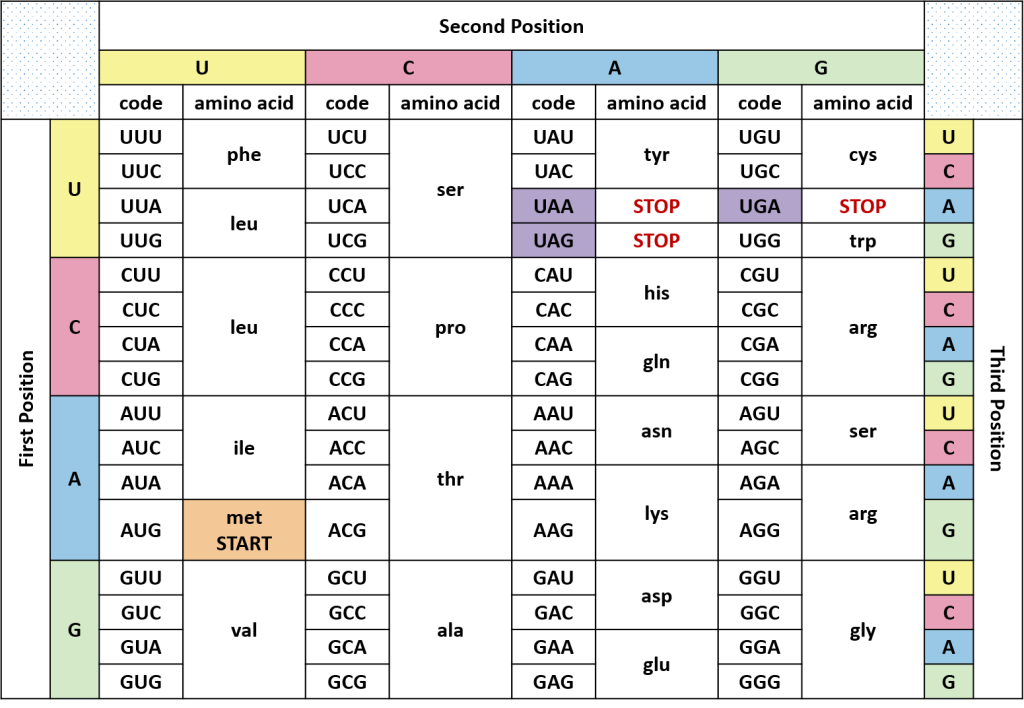
\includegraphics{images/codon.png}

\hypertarget{conclusion-6}{%
\subsection{Conclusion}\label{conclusion-6}}

In conclusion, the if and else statements in R provide bioinformaticians with the means to adapt their analyses and make data-driven decisions. By employing these control flow structures, researchers can enhance the reproducibility and adaptability of their bioinformatics workflows, ultimately advancing our understanding of biological systems. Whether you're searching for genetic elements or classifying sequences, mastering control flow is an essential skill in the bioinformatics toolbox.

\hypertarget{loops}{%
\section{Loops}\label{loops}}

In the world of data analysis and programming, loops are indispensable tools for executing repetitive tasks efficiently. They allow us to automate processes like processing multiple files or iterating through steps in an analysis pipeline. In R, we have two main types of loops: the \texttt{while} loop and the \texttt{for} loop. In this section, we'll delve into their usage with real-world examples and explore when to employ each type.

\hypertarget{the-while-loop}{%
\subsection{\texorpdfstring{The \texttt{while} Loop}{The while Loop}}\label{the-while-loop}}

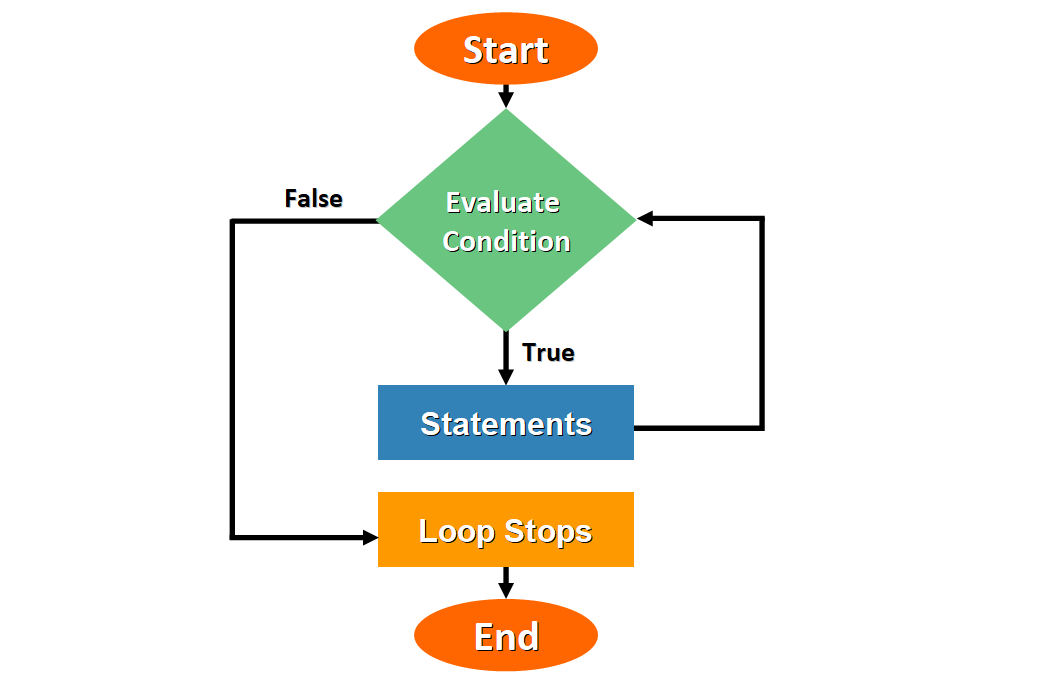
\includegraphics{images/while.png}

The \texttt{while} loop repeatedly runs a block of code as long as a specified condition remains true. A practical scenario could involve quality-controlling sequencing files one by one until we encounter a file that fails a test. Here's an example:

\begin{Shaded}
\begin{Highlighting}[]
\NormalTok{expression\_vec }\OtherTok{\textless{}{-}} \FunctionTok{c}\NormalTok{(}\DecValTok{0}\NormalTok{, }\DecValTok{4}\NormalTok{, }\DecValTok{8}\NormalTok{, }\DecValTok{16}\NormalTok{, }\DecValTok{32}\NormalTok{)}
\NormalTok{new\_expression\_vec }\OtherTok{\textless{}{-}} \FunctionTok{c}\NormalTok{()}
\NormalTok{i }\OtherTok{\textless{}{-}} \DecValTok{1}

\ControlFlowTok{while}\NormalTok{ (i }\SpecialCharTok{\textless{}=} \FunctionTok{length}\NormalTok{(expression\_vec)) \{}
\NormalTok{  expression\_value }\OtherTok{\textless{}{-}}\NormalTok{ expression\_vec[i]}
\NormalTok{  new\_expression\_vec[i] }\OtherTok{\textless{}{-}} \FunctionTok{log2}\NormalTok{(expression\_value)  }\CommentTok{\# Calculate the base{-}2 logarithm}
\NormalTok{  i }\OtherTok{\textless{}{-}}\NormalTok{ i }\SpecialCharTok{+} \DecValTok{1}  \CommentTok{\# Increment the index to process the next element}
\NormalTok{\}}

\NormalTok{new\_expression\_vec}
\end{Highlighting}
\end{Shaded}

\begin{verbatim}
## [1] -Inf    2    3    4    5
\end{verbatim}

In the given code, the loop counter \texttt{i} is initially set to 1. The while loop iterates as long as \texttt{i} is less than or equal to the length of the \texttt{expression\_vec} vector. In each iteration, it calculates the base-2 logarithm of the current element in \texttt{expression\_vec} and stores it in \texttt{new\_expression\_vec}, while incrementing the value of i by 1. This incrementing of \texttt{i} ensures that the loop processes the next element in the vector during each iteration until all elements have been processed.

Note, the calculation in R is vectorized, you can use:

\begin{Shaded}
\begin{Highlighting}[]
\FunctionTok{log2}\NormalTok{(expression\_vec)}
\end{Highlighting}
\end{Shaded}

\begin{verbatim}
## [1] -Inf    2    3    4    5
\end{verbatim}

to get the same results.

\hypertarget{while-loops-in-real-life}{%
\subsection{While Loops in Real Life}\label{while-loops-in-real-life}}

Researchers often work with large datasets generated from DNA sequencing machines. These machines produce files containing vast amounts of genetic information, and it's crucial to ensure the quality of this data before using it in further analyses. Imagine these files as a collection of books, each representing genetic information from a different sample.

To ensure that the data is reliable, scientists perform a process called quality control (QC). It's similar to checking books for errors, missing pages, or smudged ink before studying their contents. One important aspect of QC in sequencing data is assessing the quality of the readings from the sequencing machine. This quality is often represented as a \href{https://en.wikipedia.org/wiki/Phred_quality_score}{numerical score}, with higher scores indicating better data. Researchers typically set a threshold value, like a score of 30, which they consider acceptable quality.

The code snippet below (this is just a pseudo-code) illustrates how to iterate through a vector of file names, read each file, and check if the mean quality score falls below a specified threshold:

\begin{Shaded}
\begin{Highlighting}[]
\NormalTok{files }\OtherTok{\textless{}{-}} \FunctionTok{c}\NormalTok{(}\StringTok{"sample1.fq"}\NormalTok{, }\StringTok{"sample2.fq"}\NormalTok{, }\StringTok{"sample3.fq"}\NormalTok{)}
\NormalTok{i }\OtherTok{\textless{}{-}} \DecValTok{1}

\CommentTok{\# Start a \textasciigrave{}while\textasciigrave{} loop with the condition: while \textasciigrave{}i\textasciigrave{} is less than or equal to the length of \textasciigrave{}files\textasciigrave{}}
\ControlFlowTok{while}\NormalTok{ (i }\SpecialCharTok{\textless{}=} \FunctionTok{length}\NormalTok{(files)) \{}
  
  \CommentTok{\# Read the current file}
\NormalTok{  fq }\OtherTok{\textless{}{-}} \FunctionTok{readFastq}\NormalTok{(files[i])}
  
  \CommentTok{\# Check if the mean quality score is below 30}
  \ControlFlowTok{if}\NormalTok{ (}\FunctionTok{meanQual}\NormalTok{(fq) }\SpecialCharTok{\textless{}} \DecValTok{30}\NormalTok{) \{}
     \CommentTok{\# Print a failure message if the quality check fails}
     \FunctionTok{print}\NormalTok{(}\FunctionTok{paste}\NormalTok{(files[i], }\StringTok{"failed QC"}\NormalTok{))}
     \CommentTok{\# Exit the loop using \textasciigrave{}break\textasciigrave{}}
     \ControlFlowTok{break}
\NormalTok{  \} }
  
  \CommentTok{\# Increment the index \textasciigrave{}i\textasciigrave{} to move to the next file}
\NormalTok{  i }\OtherTok{\textless{}{-}}\NormalTok{ i }\SpecialCharTok{+} \DecValTok{1}
\NormalTok{\}}
\end{Highlighting}
\end{Shaded}

In this case, the loop iterates through files, reads each one, and performs quality control. If a file fails the quality check, the loop prints a failure message and exits.

\hypertarget{the-for-loop}{%
\subsection{\texorpdfstring{The \texttt{for} Loop}{The for Loop}}\label{the-for-loop}}

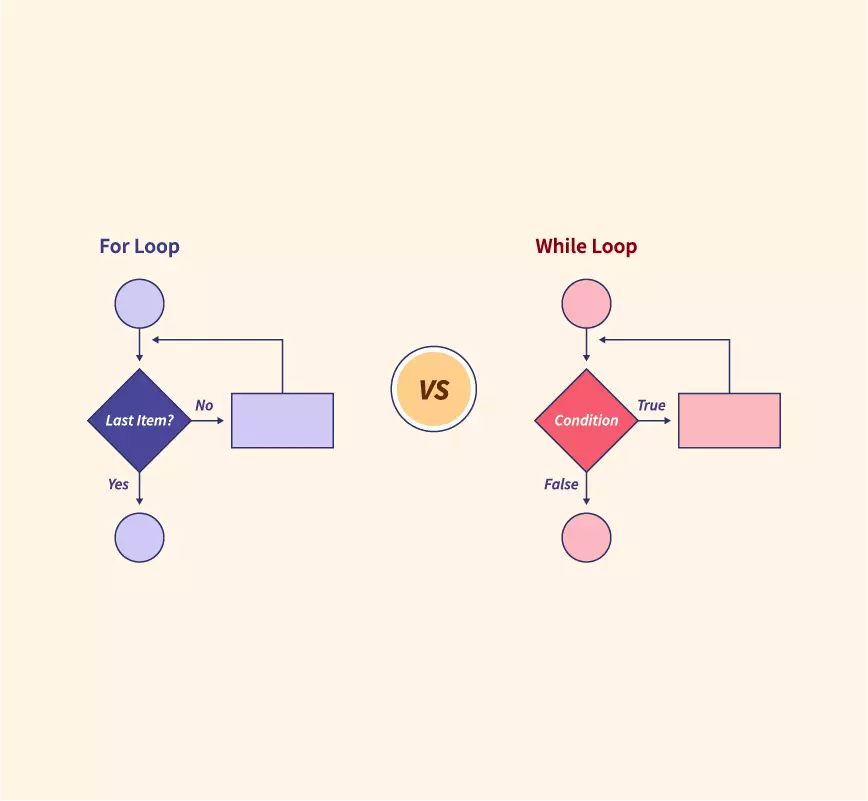
\includegraphics{images/forloop.png}

On the other hand, the for \texttt{loop} iterates through a predefined sequence of values. Consider a scenario where we want to standardize gene expression across all samples using Z-scores:

\begin{Shaded}
\begin{Highlighting}[]
\CommentTok{\# Create a matrix of gene expression data}
\NormalTok{expression\_mat }\OtherTok{\textless{}{-}} \FunctionTok{matrix}\NormalTok{(}\DecValTok{1}\SpecialCharTok{:}\DecValTok{12}\NormalTok{, }\AttributeTok{nrow =} \DecValTok{3}\NormalTok{, }\AttributeTok{ncol =} \DecValTok{4}\NormalTok{)}

\CommentTok{\# Define the row names (gene names) and column names (sample names)}
\FunctionTok{rownames}\NormalTok{(expression\_mat) }\OtherTok{\textless{}{-}} \FunctionTok{c}\NormalTok{(}\StringTok{"gene1"}\NormalTok{, }\StringTok{"gene2"}\NormalTok{, }\StringTok{"gene3"}\NormalTok{)}
\FunctionTok{colnames}\NormalTok{(expression\_mat) }\OtherTok{\textless{}{-}} \FunctionTok{c}\NormalTok{(}\StringTok{"sample1"}\NormalTok{, }\StringTok{"sample2"}\NormalTok{, }\StringTok{"sample3"}\NormalTok{, }\StringTok{"sample4"}\NormalTok{)}

\CommentTok{\# Get the gene names}
\NormalTok{genes }\OtherTok{\textless{}{-}} \FunctionTok{rownames}\NormalTok{(expression\_mat)}

\CommentTok{\# Start a for loop that iterates through each gene name \textquotesingle{}g\textquotesingle{} in \textquotesingle{}genes\textquotesingle{}}
\ControlFlowTok{for}\NormalTok{ (g }\ControlFlowTok{in}\NormalTok{ genes) \{}
  
  \CommentTok{\# Calculate the mean expression for the current gene \textquotesingle{}g\textquotesingle{}}
\NormalTok{  mean\_expr }\OtherTok{\textless{}{-}} \FunctionTok{mean}\NormalTok{(expression\_mat[g, ]) }
  
  \CommentTok{\# Calculate the standard deviation of expression for the current gene \textquotesingle{}g\textquotesingle{}}
\NormalTok{  sd\_expr }\OtherTok{\textless{}{-}} \FunctionTok{sd}\NormalTok{(expression\_mat[g, ])}
  
  \CommentTok{\# Standardize the expression values for the current gene \textquotesingle{}g\textquotesingle{} using Z{-}scores}
\NormalTok{  expression\_mat[g, ] }\OtherTok{\textless{}{-}}\NormalTok{ (expression\_mat[g, ] }\SpecialCharTok{{-}}\NormalTok{ mean\_expr) }\SpecialCharTok{/}\NormalTok{ sd\_expr}
\NormalTok{\}}

\CommentTok{\# Print the resulting standardized expression matrix \textquotesingle{}expression\_mat\textquotesingle{}}
\NormalTok{expression\_mat}
\end{Highlighting}
\end{Shaded}

\begin{verbatim}
##         sample1    sample2   sample3  sample4
## gene1 -1.161895 -0.3872983 0.3872983 1.161895
## gene2 -1.161895 -0.3872983 0.3872983 1.161895
## gene3 -1.161895 -0.3872983 0.3872983 1.161895
\end{verbatim}

In this example, the for loop efficiently iterates through each gene, calculates the mean and standard deviation of expression, and then standardizes that gene's row. This process repeats for all genes, allowing for consistent normalization.

Of course, you can use the scale function in R to do this directly without using a \texttt{for} loop. Note, \texttt{scale} works by columns. To get the same result, you need to first transpose the matrix, scale it and then transpose it back.

\begin{Shaded}
\begin{Highlighting}[]
\FunctionTok{t}\NormalTok{(}\FunctionTok{scale}\NormalTok{(}\FunctionTok{t}\NormalTok{(expression\_mat)))}
\end{Highlighting}
\end{Shaded}

\begin{verbatim}
##         sample1    sample2   sample3  sample4
## gene1 -1.161895 -0.3872983 0.3872983 1.161895
## gene2 -1.161895 -0.3872983 0.3872983 1.161895
## gene3 -1.161895 -0.3872983 0.3872983 1.161895
## attr(,"scaled:center")
## gene1 gene2 gene3 
##     0     0     0 
## attr(,"scaled:scale")
## gene1 gene2 gene3 
##     1     1     1
\end{verbatim}

\hypertarget{conclusion-7}{%
\subsection{Conclusion}\label{conclusion-7}}

It's crucial to understand that loops can provide fine-grained control for accessing and transforming data at an element level. However, in many cases, R offers vectorized operations that simplify code and make it more readable, as demonstrated with the Z-score calculation using the scale function.

Remember, \texttt{while} loops and \texttt{for} loops are valuable tools in your data analysis toolkit, but it's essential to choose the most suitable method for the task at hand. By mastering these loop structures, you can streamline your data analysis and automation processes, making your work more efficient and precise. Computers are good at repetitive work.
Whenever you are manually doing the same task multiple times, think of the loops!

\hypertarget{gene-expression-annotation-using-loops-and-control-structures}{%
\section{Gene Expression Annotation using Loops and Control Structures}\label{gene-expression-annotation-using-loops-and-control-structures}}

We often encounter scenarios where we need to categorize data based on specific criteria. In this example, we'll use a combination of loops and control structures in the R programming language to add custom annotations to gene expression measurements for a group of patients. We'll categorize their expression levels into different classes: ``not-expressed,'' ``low,'' ``medium,'' and ``high.''

\hypertarget{the-data}{%
\subsection{The Data}\label{the-data}}

Suppose we have gene expression measurements for 5 patients stored in a vector called expression\_vec. These measurements represent the expression levels of a specific gene.

\begin{Shaded}
\begin{Highlighting}[]
\NormalTok{expression\_vec }\OtherTok{\textless{}{-}} \FunctionTok{c}\NormalTok{(}\DecValTok{0}\NormalTok{, }\DecValTok{5}\NormalTok{, }\DecValTok{10}\NormalTok{, }\DecValTok{6}\NormalTok{, }\DecValTok{22}\NormalTok{)}
\end{Highlighting}
\end{Shaded}

\hypertarget{creating-annotations}{%
\subsection{Creating Annotations}\label{creating-annotations}}

We want to annotate each patient's expression status based on the range of their expression values. To do this, we'll initiate an empty vector called \texttt{annotations} to store our annotations.

\begin{Shaded}
\begin{Highlighting}[]
\NormalTok{annotations }\OtherTok{\textless{}{-}} \FunctionTok{c}\NormalTok{()}
\end{Highlighting}
\end{Shaded}

Now, let's go through the process step by step.

\hypertarget{the-loop}{%
\subsection{The Loop}\label{the-loop}}

\begin{Shaded}
\begin{Highlighting}[]
\ControlFlowTok{for}\NormalTok{ (expression\_value }\ControlFlowTok{in}\NormalTok{ expression\_vec) \{}
  \ControlFlowTok{if}\NormalTok{ (expression\_value }\SpecialCharTok{==} \DecValTok{0}\NormalTok{) \{}
\NormalTok{    annotation }\OtherTok{\textless{}{-}} \StringTok{"not{-}expressed"} 
\NormalTok{  \} }\ControlFlowTok{else} \ControlFlowTok{if}\NormalTok{ (expression\_value }\SpecialCharTok{\textgreater{}} \DecValTok{0} \SpecialCharTok{\&}\NormalTok{ expression\_value }\SpecialCharTok{\textless{}} \DecValTok{5}\NormalTok{) \{}
\NormalTok{    annotation }\OtherTok{\textless{}{-}} \StringTok{"low"}
\NormalTok{  \} }\ControlFlowTok{else} \ControlFlowTok{if}\NormalTok{ (expression\_value }\SpecialCharTok{\textgreater{}=} \DecValTok{5} \SpecialCharTok{\&}\NormalTok{ expression\_value }\SpecialCharTok{\textless{}} \DecValTok{20}\NormalTok{) \{}
\NormalTok{    annotation }\OtherTok{\textless{}{-}} \StringTok{"medium"}
\NormalTok{  \} }\ControlFlowTok{else}\NormalTok{ \{}
\NormalTok{    annotation }\OtherTok{\textless{}{-}} \StringTok{"high"}
\NormalTok{  \}}
\NormalTok{  annotations }\OtherTok{\textless{}{-}} \FunctionTok{c}\NormalTok{(annotations, annotation)}
\NormalTok{\}}
\end{Highlighting}
\end{Shaded}

Here's what's happening in the code:

\begin{itemize}
\item
  We use a for loop to iterate through each expression\_value in the expression\_vec vector.
\item
  Inside the loop, we use a series of if and else if statements to categorize each expression\_value based on its range.
\item
  If the value is exactly 0, we assign the annotation ``not-expressed.''
\item
  If the value is greater than 0 but less than 5, we assign the annotation ``low.''
\item
  If the value is greater than or equal to 5 but less than 20, we assign the annotation ``medium.''
\item
  If none of the above conditions are met, we assign the annotation ``high.''
\item
  Finally, we append each annotation to the annotations vector.
\end{itemize}

\hypertarget{output}{%
\subsection{Output}\label{output}}

Let's see the results of our annotations:

\begin{Shaded}
\begin{Highlighting}[]
\NormalTok{annotations}
\end{Highlighting}
\end{Shaded}

\begin{verbatim}
## [1] "not-expressed" "medium"        "medium"        "medium"       
## [5] "high"
\end{verbatim}

\hypertarget{putting-it-all-together}{%
\subsection{Putting it all together}\label{putting-it-all-together}}

\begin{Shaded}
\begin{Highlighting}[]
\NormalTok{expression\_vec}\OtherTok{\textless{}{-}} \FunctionTok{c}\NormalTok{(}\DecValTok{0}\NormalTok{, }\DecValTok{5}\NormalTok{, }\DecValTok{10}\NormalTok{, }\DecValTok{6}\NormalTok{, }\DecValTok{22}\NormalTok{)}

\CommentTok{\# initiate an empty vector }
\NormalTok{annotations }\OtherTok{\textless{}{-}} \FunctionTok{c}\NormalTok{() }

\ControlFlowTok{for}\NormalTok{ (expression\_value }\ControlFlowTok{in}\NormalTok{ expression\_vec)\{}
  \ControlFlowTok{if}\NormalTok{ ( expression\_value }\SpecialCharTok{==}\DecValTok{0}\NormalTok{ )\{}
\NormalTok{    annotation }\OtherTok{\textless{}{-}} \StringTok{"not{-}expressed"} 
\NormalTok{    \} }\ControlFlowTok{else} \ControlFlowTok{if}\NormalTok{ (expression\_value }\SpecialCharTok{\textgreater{}}\DecValTok{0} \SpecialCharTok{\&}\NormalTok{ expression\_value }\SpecialCharTok{\textless{}} \DecValTok{5}\NormalTok{) \{}
\NormalTok{      annotation}\OtherTok{\textless{}{-}} \StringTok{"low"}
\NormalTok{    \} }\ControlFlowTok{else} \ControlFlowTok{if}\NormalTok{ (expression\_value }\SpecialCharTok{\textgreater{}=}\DecValTok{5} \SpecialCharTok{\&}\NormalTok{ expression\_value }\SpecialCharTok{\textless{}}\DecValTok{20}\NormalTok{) \{}
\NormalTok{      annotation}\OtherTok{\textless{}{-}} \StringTok{"medium"}
\NormalTok{    \} }\ControlFlowTok{else}\NormalTok{ \{}
\NormalTok{      annotation}\OtherTok{\textless{}{-}} \StringTok{"high"}
\NormalTok{    \}}
\NormalTok{    annotations}\OtherTok{\textless{}{-}} \FunctionTok{c}\NormalTok{(annotations, annotation)}
\NormalTok{  \}}

\NormalTok{annotations}
\end{Highlighting}
\end{Shaded}

\begin{verbatim}
## [1] "not-expressed" "medium"        "medium"        "medium"       
## [5] "high"
\end{verbatim}

In R, everything is vectorized. There is a much better way to achieve the same thing using the \href{https://dplyr.tidyverse.org/reference/case_when.html}{\texttt{case\_when}} function in the \texttt{dplyr} package. We will cover it in the later lecture.

\hypertarget{conclusion-8}{%
\subsection{Conclusion}\label{conclusion-8}}

This approach to categorizing gene expression data is essential in various biological and medical research contexts. For example:

\begin{itemize}
\item
  Drug Development: When studying the impact of a drug on gene expression, researchers need to categorize gene expression levels to assess the drug's effectiveness.
\item
  Cancer Research: Identifying genes with high or low expression levels can provide insights into cancer progression and potential therapeutic targets.
\item
  Disease Biomarker Discovery: Categorizing gene expression in patients with a specific disease can help identify biomarkers for early diagnosis.
\end{itemize}

By combining loops and control structures as shown in this example, scientists and analysts can efficiently handle and interpret complex biological data.

\hypertarget{lets-solve-a-challenge}{%
\section{Let's solve a Challenge}\label{lets-solve-a-challenge}}

You're given a vector of daily average temperatures (in Celsius) for a month. Your task is to analyze the temperature data to find out the following:

\begin{itemize}
\item
  The number of days with temperatures above the monthly average.
\item
  Whether any day's temperature exceeds 30°C (considering it as a threshold for a very hot day).
\item
  The number of days with temperatures below 15°C (considering it as a threshold for a cold day).
\end{itemize}

Given Data:

\begin{Shaded}
\begin{Highlighting}[]
\NormalTok{temperatures }\OtherTok{\textless{}{-}} \FunctionTok{c}\NormalTok{(}\DecValTok{12}\NormalTok{, }\DecValTok{14}\NormalTok{, }\DecValTok{16}\NormalTok{, }\DecValTok{20}\NormalTok{, }\DecValTok{22}\NormalTok{, }\DecValTok{24}\NormalTok{, }\DecValTok{26}\NormalTok{, }\DecValTok{28}\NormalTok{, }\DecValTok{30}\NormalTok{, }\DecValTok{32}\NormalTok{, }\DecValTok{18}\NormalTok{, }\DecValTok{16}\NormalTok{, }\DecValTok{14}\NormalTok{, }\DecValTok{22}\NormalTok{, }\DecValTok{24}\NormalTok{, }\DecValTok{26}\NormalTok{, }\DecValTok{20}\NormalTok{, }\DecValTok{18}\NormalTok{, }\DecValTok{17}\NormalTok{, }\DecValTok{15}\NormalTok{, }\DecValTok{13}\NormalTok{, }\DecValTok{11}\NormalTok{, }\DecValTok{9}\NormalTok{, }\DecValTok{7}\NormalTok{, }\DecValTok{5}\NormalTok{, }\DecValTok{8}\NormalTok{, }\DecValTok{10}\NormalTok{, }\DecValTok{12}\NormalTok{, }\DecValTok{14}\NormalTok{, }\DecValTok{16}\NormalTok{)}
\end{Highlighting}
\end{Shaded}

Tasks:

\begin{enumerate}
\def\labelenumi{\arabic{enumi}.}
\item
  Calculate the monthly average temperature.
\item
  Use a loop to iterate through the temperatures vector.
\end{enumerate}

\begin{itemize}
\item
  For each temperature, check if it's above the monthly average and count these occurrences.
\item
  Check if there's any day with a temperature exceeding 30°C.
\item
  Count the number of days with temperatures below 15°C.
\end{itemize}

\begin{enumerate}
\def\labelenumi{\arabic{enumi}.}
\setcounter{enumi}{2}
\tightlist
\item
  Print the results:
\end{enumerate}

\begin{itemize}
\item
  Total number of days above the monthly average.
\item
  Whether there was a very hot day (temperature \textgreater{} 30°C).
\item
  Number of cold days (temperature \textless{} 15°C).
\end{itemize}

\hypertarget{solution}{%
\section{Solution}\label{solution}}

Before diving into the solution, I encourage all students to take a moment to challenge themselves and attempt to solve the problem independently. This coding exercise provides a valuable opportunity to practice essential programming concepts in R, such as loops, conditional statements, and basic data manipulation. Start by considering how you would calculate the monthly average temperature from a list of daily temperatures and how you might track the number of days above the average, very hot days (above 30°C), and cold days (below 15°C). Once you've given it a try, feel free to compare your approach with the provided solution to deepen your understanding and refine your coding skills. Happy coding!

\hypertarget{using-a-for-loop}{%
\subsection{using a for loop}\label{using-a-for-loop}}

\begin{Shaded}
\begin{Highlighting}[]
\CommentTok{\# Given data: Daily average temperatures for a month (in Celsius)}
\NormalTok{temperatures }\OtherTok{\textless{}{-}} \FunctionTok{c}\NormalTok{(}\DecValTok{12}\NormalTok{, }\DecValTok{14}\NormalTok{, }\DecValTok{16}\NormalTok{, }\DecValTok{20}\NormalTok{, }\DecValTok{22}\NormalTok{, }\DecValTok{24}\NormalTok{, }\DecValTok{26}\NormalTok{, }\DecValTok{28}\NormalTok{, }\DecValTok{30}\NormalTok{, }\DecValTok{32}\NormalTok{, }\DecValTok{18}\NormalTok{, }\DecValTok{16}\NormalTok{, }\DecValTok{14}\NormalTok{, }\DecValTok{22}\NormalTok{, }\DecValTok{24}\NormalTok{, }\DecValTok{26}\NormalTok{, }\DecValTok{20}\NormalTok{, }\DecValTok{18}\NormalTok{, }\DecValTok{17}\NormalTok{, }\DecValTok{15}\NormalTok{, }\DecValTok{13}\NormalTok{, }\DecValTok{11}\NormalTok{, }\DecValTok{9}\NormalTok{, }\DecValTok{7}\NormalTok{, }\DecValTok{5}\NormalTok{, }\DecValTok{8}\NormalTok{, }\DecValTok{10}\NormalTok{, }\DecValTok{12}\NormalTok{, }\DecValTok{14}\NormalTok{, }\DecValTok{16}\NormalTok{)}

\CommentTok{\# Manually calculate the monthly average temperature}
\NormalTok{total\_temperature }\OtherTok{\textless{}{-}} \DecValTok{0}  \CommentTok{\# Initialize a variable to hold the sum of all temperatures}
\ControlFlowTok{for}\NormalTok{ (temp }\ControlFlowTok{in}\NormalTok{ temperatures) \{}
\NormalTok{  total\_temperature }\OtherTok{\textless{}{-}}\NormalTok{ total\_temperature }\SpecialCharTok{+}\NormalTok{ temp  }\CommentTok{\# Accumulate the total temperature}
\NormalTok{\}}
\NormalTok{monthly\_average }\OtherTok{\textless{}{-}}\NormalTok{ total\_temperature }\SpecialCharTok{/} \FunctionTok{length}\NormalTok{(temperatures)  }\CommentTok{\# Divide by the number of temperatures to get the average}
\FunctionTok{print}\NormalTok{(}\FunctionTok{paste}\NormalTok{(}\StringTok{"Monthly average temperature:"}\NormalTok{, monthly\_average, }\StringTok{"C"}\NormalTok{))}
\end{Highlighting}
\end{Shaded}

\begin{verbatim}
## [1] "Monthly average temperature: 17.3 C"
\end{verbatim}

\begin{Shaded}
\begin{Highlighting}[]
\CommentTok{\# Initialize counters for the conditions}
\NormalTok{days\_above\_average }\OtherTok{\textless{}{-}} \DecValTok{0}
\NormalTok{very\_hot\_days }\OtherTok{\textless{}{-}} \DecValTok{0}
\NormalTok{cold\_days }\OtherTok{\textless{}{-}} \DecValTok{0}

\CommentTok{\# Use a loop to iterate through the temperatures vector}
\ControlFlowTok{for}\NormalTok{ (temp }\ControlFlowTok{in}\NormalTok{ temperatures) \{}
  \CommentTok{\# Check if the temperature is above the monthly average}
  \ControlFlowTok{if}\NormalTok{ (temp }\SpecialCharTok{\textgreater{}}\NormalTok{ monthly\_average) \{}
\NormalTok{    days\_above\_average }\OtherTok{\textless{}{-}}\NormalTok{ days\_above\_average }\SpecialCharTok{+} \DecValTok{1}
\NormalTok{  \}}
  
  \CommentTok{\# Check if the temperature exceeds 30°C (very hot day)}
  \ControlFlowTok{if}\NormalTok{ (temp }\SpecialCharTok{\textgreater{}} \DecValTok{30}\NormalTok{) \{}
\NormalTok{    very\_hot\_days }\OtherTok{\textless{}{-}}\NormalTok{ very\_hot\_days }\SpecialCharTok{+} \DecValTok{1}
\NormalTok{  \}}
  
  \CommentTok{\# Check if the temperature is below 15°C (cold day)}
  \ControlFlowTok{if}\NormalTok{ (temp }\SpecialCharTok{\textless{}} \DecValTok{15}\NormalTok{) \{}
\NormalTok{    cold\_days }\OtherTok{\textless{}{-}}\NormalTok{ cold\_days }\SpecialCharTok{+} \DecValTok{1}
\NormalTok{  \}}
\NormalTok{\}}

\CommentTok{\# Print the results}
\FunctionTok{print}\NormalTok{(}\FunctionTok{paste}\NormalTok{(}\StringTok{"Number of days above the monthly average:"}\NormalTok{, days\_above\_average))}
\end{Highlighting}
\end{Shaded}

\begin{verbatim}
## [1] "Number of days above the monthly average: 13"
\end{verbatim}

\begin{Shaded}
\begin{Highlighting}[]
\FunctionTok{print}\NormalTok{(}\FunctionTok{paste}\NormalTok{(}\StringTok{"Number of very hot days (temperature \textgreater{} 30°C):"}\NormalTok{, very\_hot\_days))}
\end{Highlighting}
\end{Shaded}

\begin{verbatim}
## [1] "Number of very hot days (temperature > 30°C): 1"
\end{verbatim}

\begin{Shaded}
\begin{Highlighting}[]
\FunctionTok{print}\NormalTok{(}\FunctionTok{paste}\NormalTok{(}\StringTok{"Number of cold days (temperature \textless{} 15°C):"}\NormalTok{, cold\_days))}
\end{Highlighting}
\end{Shaded}

\begin{verbatim}
## [1] "Number of cold days (temperature < 15°C): 12"
\end{verbatim}

In this solution, we start with a list of daily average temperatures for a month, stored in the `temperatures' vector. The first part of the code calculates the monthly average temperature by adding up all the daily temperatures and then dividing the total by the number of days in the month. We use a loop to go through each temperature, adding it to the `total\_temperature' variable. Once we have the sum, we divide it by the number of days to find the average and print it using the `cat' function.

The second part of the code uses loops and conditional statements to analyze the temperatures. It tracks three things: the number of days with temperatures above the monthly average, the number of very hot days (where the temperature is above 30°C), and the number of cold days (where the temperature is below 15°C). For each temperature in the `temperatures' vector, the code checks if it's above the monthly average, above 30°C, or below 15°C, and increments the corresponding counter if the condition is met. Finally, the code prints out the results using `paste', displaying the count of days for each condition.

\hypertarget{vectorized-solution}{%
\subsection{vectorized solution}\label{vectorized-solution}}

The solution shown here is how you usually solve the problem in python. However, as I introduced earlier, R is vectorized, many of the calculations can be simplified.

\begin{Shaded}
\begin{Highlighting}[]
\NormalTok{temperatures }\OtherTok{\textless{}{-}} \FunctionTok{c}\NormalTok{(}\DecValTok{12}\NormalTok{, }\DecValTok{14}\NormalTok{, }\DecValTok{16}\NormalTok{, }\DecValTok{20}\NormalTok{, }\DecValTok{22}\NormalTok{, }\DecValTok{24}\NormalTok{, }\DecValTok{26}\NormalTok{, }\DecValTok{28}\NormalTok{, }\DecValTok{30}\NormalTok{, }\DecValTok{32}\NormalTok{, }\DecValTok{18}\NormalTok{, }\DecValTok{16}\NormalTok{, }\DecValTok{14}\NormalTok{, }\DecValTok{22}\NormalTok{, }\DecValTok{24}\NormalTok{, }\DecValTok{26}\NormalTok{, }\DecValTok{20}\NormalTok{, }\DecValTok{18}\NormalTok{, }\DecValTok{17}\NormalTok{, }\DecValTok{15}\NormalTok{, }\DecValTok{13}\NormalTok{, }\DecValTok{11}\NormalTok{, }\DecValTok{9}\NormalTok{, }\DecValTok{7}\NormalTok{, }\DecValTok{5}\NormalTok{, }\DecValTok{8}\NormalTok{, }\DecValTok{10}\NormalTok{, }\DecValTok{12}\NormalTok{, }\DecValTok{14}\NormalTok{, }\DecValTok{16}\NormalTok{)}

\NormalTok{monthly\_average}\OtherTok{\textless{}{-}} \FunctionTok{mean}\NormalTok{(temperatures)}

\NormalTok{monthly\_average}
\end{Highlighting}
\end{Shaded}

\begin{verbatim}
## [1] 17.3
\end{verbatim}

\begin{Shaded}
\begin{Highlighting}[]
\CommentTok{\# get a logical vector}
\NormalTok{very\_hot\_days\_lgl}\OtherTok{\textless{}{-}}\NormalTok{ temperatures }\SpecialCharTok{\textgreater{}} \DecValTok{30}

\NormalTok{very\_hot\_days\_lgl}
\end{Highlighting}
\end{Shaded}

\begin{verbatim}
##  [1] FALSE FALSE FALSE FALSE FALSE FALSE FALSE FALSE FALSE  TRUE FALSE FALSE
## [13] FALSE FALSE FALSE FALSE FALSE FALSE FALSE FALSE FALSE FALSE FALSE FALSE
## [25] FALSE FALSE FALSE FALSE FALSE FALSE
\end{verbatim}

\begin{Shaded}
\begin{Highlighting}[]
\CommentTok{\# remember in R, FALSE is 0 and TRUE is 1 under the hood. you can sum it up to }
\CommentTok{\# find how many are TRUE}
\NormalTok{very\_hot\_days}\OtherTok{\textless{}{-}} \FunctionTok{sum}\NormalTok{(very\_hot\_days\_lgl)}
\NormalTok{very\_hot\_days}
\end{Highlighting}
\end{Shaded}

\begin{verbatim}
## [1] 1
\end{verbatim}

Similarly, you can

\begin{Shaded}
\begin{Highlighting}[]
\NormalTok{cold\_days}\OtherTok{\textless{}{-}} \FunctionTok{sum}\NormalTok{(temperatures }\SpecialCharTok{\textless{}} \DecValTok{15}\NormalTok{)}
\NormalTok{cold\_days}
\end{Highlighting}
\end{Shaded}

\begin{verbatim}
## [1] 12
\end{verbatim}

You see how powerful R is when combining the logical vector and its vectorized feature!

\hypertarget{section-complete}{%
\section{Section complete}\label{section-complete}}

Congratulations on completing this section of our course! You've made significant progress in understanding the essentials of boolean operators, control flow with if statements, and the power of loops. These foundational skills are crucial for analyzing data, automating tasks, and making logical decisions in your code. It's impressive how much you've learned and can now apply to real-world problems, from gene expression analysis to data quality control and beyond.

Keep this momentum going as you move forward. The concepts you've mastered here will serve as building blocks for more advanced programming techniques and analytical methods. Remember, practice is key to deepening your understanding and honing your skills. Let's move on to the next section.

\hypertarget{going-more-in-depth-with-r}{%
\chapter{Going more in-depth with R}\label{going-more-in-depth-with-r}}

\hypertarget{handling-missing-values}{%
\section{Handling Missing Values}\label{handling-missing-values}}

In bioinformatics, dealing with missing data is a common challenge. Missing values can arise from various sources, including experimental limitations or data collection errors. It's crucial to understand how to identify and handle these missing values effectively to ensure the accuracy of your analyses. In R, missing values are represented by \texttt{NA}, indicating the absence of a value. In this tutorial, we will explore key properties of \texttt{NA}, learn how to identify missing values, and discover techniques to handle them in your gene expression datasets.

\hypertarget{understanding-na-in-r}{%
\subsection{Understanding NA in R}\label{understanding-na-in-r}}

\hypertarget{propagation-of-na}{%
\subsubsection{\texorpdfstring{Propagation of \texttt{NA}:}{Propagation of NA:}}\label{propagation-of-na}}

When performing operations on vectors or data frames, most functions in R will propagate \texttt{NA} values. This means that if even a single element within a vector is \texttt{NA}, the result of the operation will also be \texttt{NA}. For example:

\begin{Shaded}
\begin{Highlighting}[]
\CommentTok{\# Example vector with missing values}
\NormalTok{gene\_expression }\OtherTok{\textless{}{-}} \FunctionTok{c}\NormalTok{(}\DecValTok{10}\NormalTok{, }\DecValTok{15}\NormalTok{, }\ConstantTok{NA}\NormalTok{, }\DecValTok{25}\NormalTok{, }\DecValTok{18}\NormalTok{, }\ConstantTok{NA}\NormalTok{, }\DecValTok{30}\NormalTok{)}

\CommentTok{\# Performing a calculation on the vector}
\NormalTok{result }\OtherTok{\textless{}{-}}\NormalTok{ gene\_expression }\SpecialCharTok{*} \DecValTok{2}

\NormalTok{result}
\end{Highlighting}
\end{Shaded}

\begin{verbatim}
## [1] 20 30 NA 50 36 NA 60
\end{verbatim}

As you can see, the presence of \texttt{NA} in the \texttt{gene\_expression} vector leads to \texttt{NA} values in the result vector.

\hypertarget{handling-na-in-summary-statistics}{%
\subsubsection{Handling NA in Summary Statistics}\label{handling-na-in-summary-statistics}}

By default, \texttt{NA} values are omitted from summary statistics like the mean, median, or standard deviation. However, specialized functions often allow you to handle \texttt{NA} values explicitly using the na.rm parameter. For instance:

\begin{Shaded}
\begin{Highlighting}[]
\CommentTok{\# Calculate the mean, ignoring NA values}
\NormalTok{mean\_expression }\OtherTok{\textless{}{-}} \FunctionTok{mean}\NormalTok{(gene\_expression, }\AttributeTok{na.rm =} \ConstantTok{TRUE}\NormalTok{)}
\NormalTok{mean\_expression}
\end{Highlighting}
\end{Shaded}

\begin{verbatim}
## [1] 19.6
\end{verbatim}

\begin{Shaded}
\begin{Highlighting}[]
\CommentTok{\# NA propgates}
\NormalTok{mean\_expression }\OtherTok{\textless{}{-}} \FunctionTok{mean}\NormalTok{(gene\_expression)}
\NormalTok{mean\_expression}
\end{Highlighting}
\end{Shaded}

\begin{verbatim}
## [1] NA
\end{verbatim}

\hypertarget{identifying-missing-values}{%
\subsection{Identifying Missing Values}\label{identifying-missing-values}}

To identify missing values in your data, you can use the \texttt{is.na()} function. It returns a logical vector where \texttt{TRUE} indicates a missing value. For example:

\begin{Shaded}
\begin{Highlighting}[]
\CommentTok{\# Identify missing values}
\NormalTok{missing\_values }\OtherTok{\textless{}{-}} \FunctionTok{is.na}\NormalTok{(gene\_expression)}

\NormalTok{missing\_values}
\end{Highlighting}
\end{Shaded}

\begin{verbatim}
## [1] FALSE FALSE  TRUE FALSE FALSE  TRUE FALSE
\end{verbatim}

\hypertarget{remove-missing-values}{%
\subsection{remove missing values}\label{remove-missing-values}}

Now, let's explore how to handle missing values in your gene expression dataset. Suppose you want to remove missing values to clean your data. You can do this using subsetting with the logical vector we created earlier:

\begin{Shaded}
\begin{Highlighting}[]
\CommentTok{\# Remove missing values}
\NormalTok{clean\_data }\OtherTok{\textless{}{-}}\NormalTok{ gene\_expression[}\SpecialCharTok{!}\NormalTok{missing\_values]}

\NormalTok{clean\_data}
\end{Highlighting}
\end{Shaded}

\begin{verbatim}
## [1] 10 15 25 18 30
\end{verbatim}

The \texttt{clean\_data} vector now contains only the non-missing values from the original \texttt{gene\_expression} vector.

\hypertarget{real-life-note}{%
\subsection{real-life note}\label{real-life-note}}

In real life, the data are usually messy. People use different ways to represent missing values. It can be \texttt{-}, \texttt{N/A}, \texttt{NULL} etc. see below

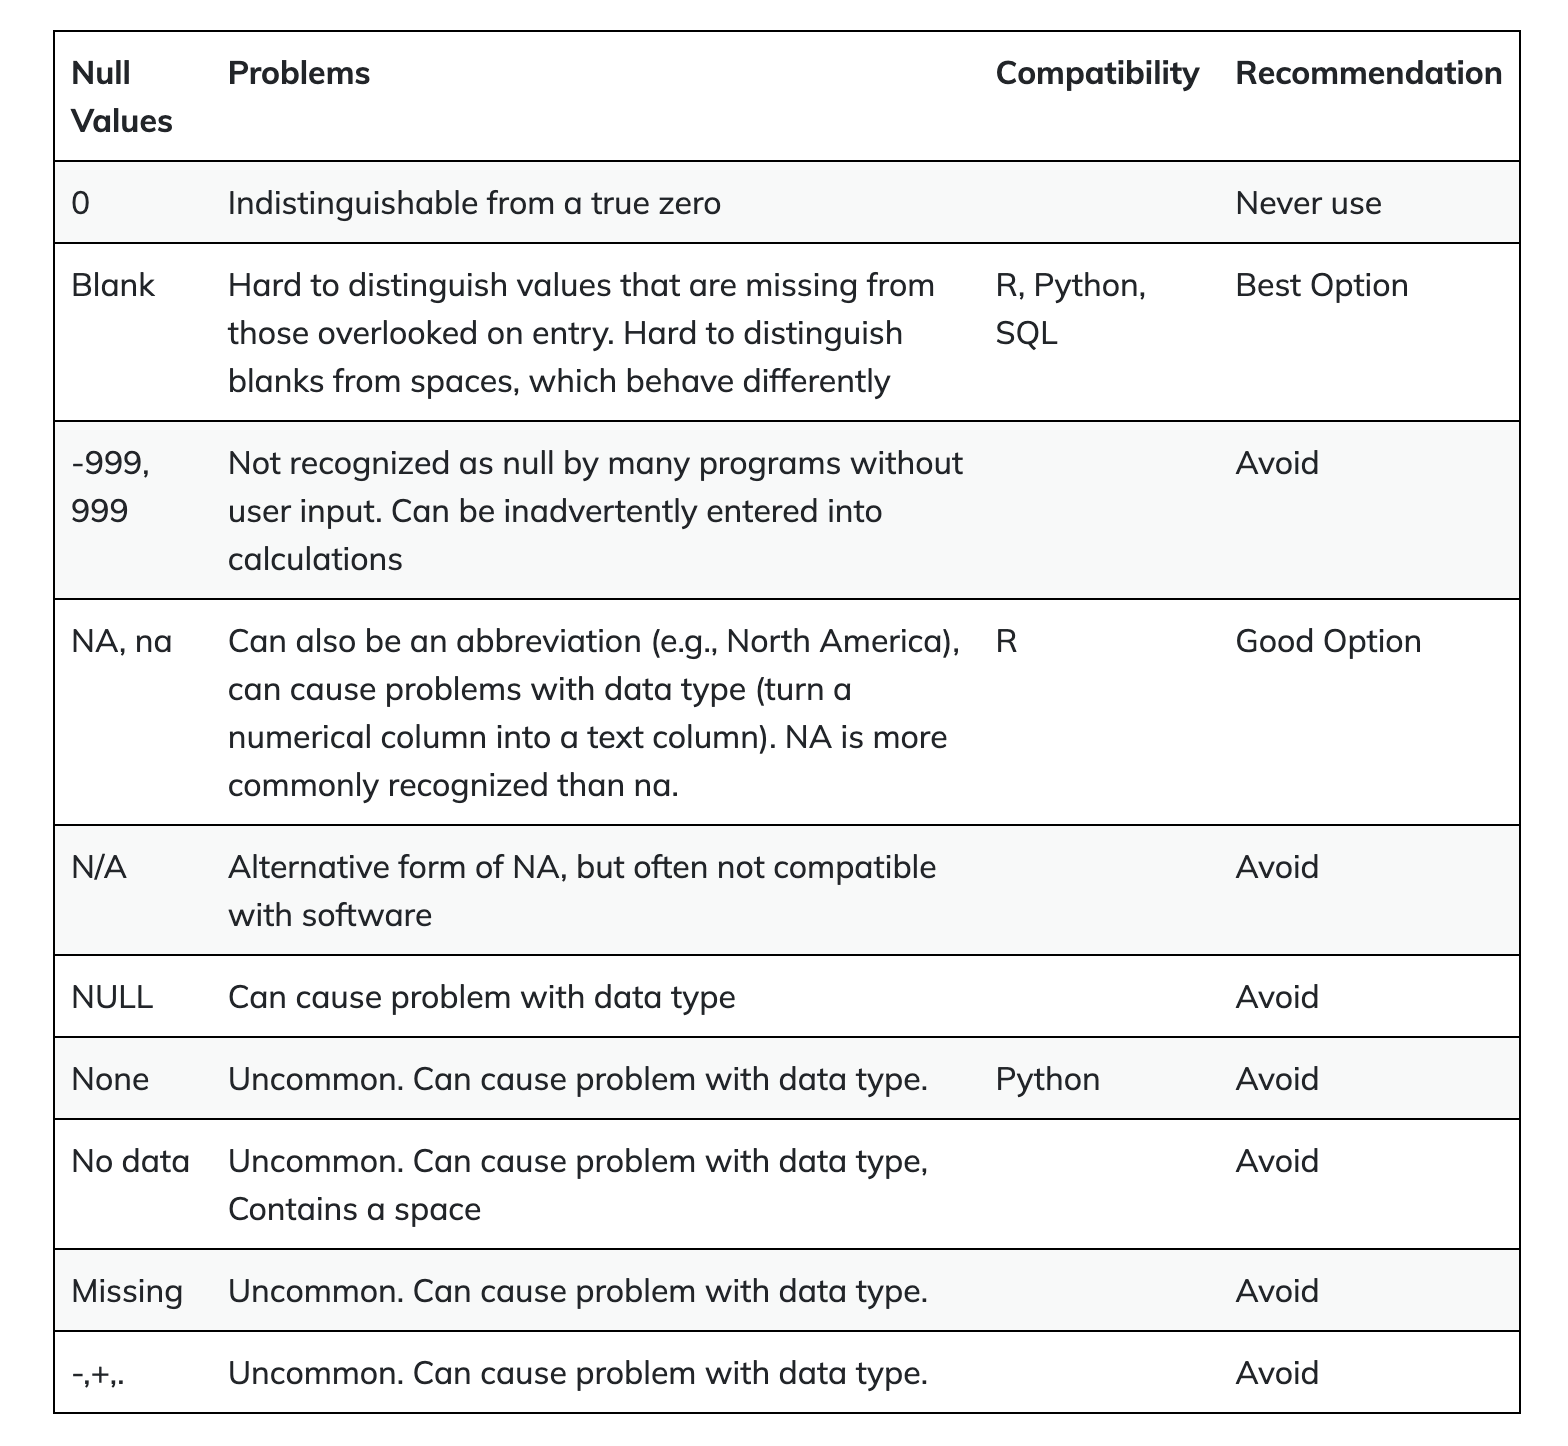
\includegraphics{images/NA.png}

More often, you have data in a dataframe. You can use the \texttt{table(df\$column\_name,\ useNA="ifany")} function to check all the possible values and you will spot the \texttt{NAs}.

See this old post from me \url{https://rpubs.com/crazyhottommy/when_NA_is_not_NA}

\hypertarget{conclusion-9}{%
\subsection{Conclusion}\label{conclusion-9}}

Handling missing values is a crucial skill in bioinformatics, as it ensures the reliability of your analyses. Whether you're calculating summary statistics or performing complex analyses, understanding how to work with missing data is an essential part of your bioinformatics toolkit.

\hypertarget{introduction-to-statistical-tests-and-p-values}{%
\section{Introduction to Statistical Tests and P-Values}\label{introduction-to-statistical-tests-and-p-values}}

We often need to determine whether there are significant differences between groups of data. Let's consider a scenario where we have two sets of cells: a control group and a treatment group (which could represent various treatments like chemical or radiation exposure). Our goal is to assess if a particular gene, let's call it Gene A, exhibits differential expression under treatment conditions. Each group has 12 replicates.

We typically start with a null hypothesis (H0), which suggests that there is no difference in gene expression for Gene A after treatment, and an alternative hypothesis (H1), which suggests that Gene A's expression changes after treatment.

Now, we perform a statistical test, like the t-test, on the averages of the two groups. If the test yields a p-value, say p = 0.035, and we've set a significance threshold (alpha) of 0.05, we compare these values. A p-value of 0.035 is less than 0.05, which leads us to reject the null hypothesis, concluding that Gene A's expression significantly changes after treatment.

\begin{quote}
But what does a p-value of 0.035 really mean?
\end{quote}

A p-value starts with the assumption that the null hypothesis is true. In this context, a p-value of 0.035 means that under the null hypothesis, the probability of observing the observed difference in gene expression after treatment is 0.035, which is quite low. By selecting a significance level of 0.05, we establish a threshold for significance. When the p-value falls below this threshold, we reject the null hypothesis in favor of the alternative hypothesis. Thus, understanding the null hypothesis is crucial for interpreting the p-value's significance.

\hypertarget{practical-application-of-statistical-test-with-r}{%
\subsection{Practical Application of statistical test with R}\label{practical-application-of-statistical-test-with-r}}

Let's dive deeper into t-tests and their practical application using R:

\hypertarget{two-sample-t-test}{%
\subsubsection{Two-Sample t-Test}\label{two-sample-t-test}}

In bioinformatics, the two-sample t-test is a valuable tool for comparing the means of two groups when you have continuous data, such as gene expression levels. It assesses whether the difference between the two group means is statistically significant.

Let's consider an example with two sets of gene expression data, `condition1' and `condition2':

\begin{Shaded}
\begin{Highlighting}[]
\CommentTok{\# Gene expression data for two conditions}
\NormalTok{condition1 }\OtherTok{\textless{}{-}} \FunctionTok{c}\NormalTok{(}\DecValTok{12}\NormalTok{, }\DecValTok{15}\NormalTok{, }\DecValTok{20}\NormalTok{, }\DecValTok{25}\NormalTok{)}
\NormalTok{condition2 }\OtherTok{\textless{}{-}} \FunctionTok{c}\NormalTok{(}\DecValTok{8}\NormalTok{, }\DecValTok{10}\NormalTok{, }\DecValTok{7}\NormalTok{, }\DecValTok{9}\NormalTok{)}

\CommentTok{\# Perform a two{-}sample t{-}test}
\NormalTok{t\_test\_result }\OtherTok{\textless{}{-}} \FunctionTok{t.test}\NormalTok{(condition1, condition2)}
\NormalTok{t\_test\_result}
\end{Highlighting}
\end{Shaded}

\begin{verbatim}
## 
##  Welch Two Sample t-test
## 
## data:  condition1 and condition2
## t = 3.2426, df = 3.3053, p-value = 0.04159
## alternative hypothesis: true difference in means is not equal to 0
## 95 percent confidence interval:
##   0.6450826 18.3549174
## sample estimates:
## mean of x mean of y 
##      18.0       8.5
\end{verbatim}

In this example, the t-test yields a p-value of 0.04159. This p-value represents the probability of observing the difference in gene expression between `condition1' and `condition2' if the null hypothesis were true (i.e., no difference). Since 0.04159 is less than the typical significance level of 0.05, we reject the null hypothesis, indicating that there is a statistically significant difference in gene expression between the two conditions.

\hypertarget{one-sided-t-test}{%
\subsubsection{One-Sided t-Test}\label{one-sided-t-test}}

In some cases, you may be interested in whether one group's mean is greater than the other. This is where one-sided t-tests come into play.

\begin{Shaded}
\begin{Highlighting}[]
\CommentTok{\# Perform a one{-}sided t{-}test (condition1 \textgreater{} condition2)}
\FunctionTok{t.test}\NormalTok{(condition1, condition2, }\AttributeTok{alternative =} \StringTok{"greater"}\NormalTok{)}
\end{Highlighting}
\end{Shaded}

\begin{verbatim}
## 
##  Welch Two Sample t-test
## 
## data:  condition1 and condition2
## t = 3.2426, df = 3.3053, p-value = 0.0208
## alternative hypothesis: true difference in means is greater than 0
## 95 percent confidence interval:
##  2.857331      Inf
## sample estimates:
## mean of x mean of y 
##      18.0       8.5
\end{verbatim}

In this example, the p-value is 0.0208. This test specifically checks if the gene expression in `condition1' is greater than in `condition2'. By specifying the `alternative' parameter as `greater,' we focus our test on this direction. Again, the p-value is compared to the significance level to make a determination.

\hypertarget{non-parametric-test}{%
\subsubsection{Non-Parametric Test}\label{non-parametric-test}}

The t-test assumes that the data follows a normal distribution. If this assumption is not met, you can use non-parametric tests like the Wilcoxon rank-sum test.

\begin{Shaded}
\begin{Highlighting}[]
\FunctionTok{wilcox.test}\NormalTok{(condition1, condition2)}
\end{Highlighting}
\end{Shaded}

\begin{verbatim}
## 
##  Wilcoxon rank sum exact test
## 
## data:  condition1 and condition2
## W = 16, p-value = 0.02857
## alternative hypothesis: true location shift is not equal to 0
\end{verbatim}

In this example, the p-value is 0.02857. The Wilcoxon rank-sum test is valuable when your data doesn't meet the normality assumption, making it a robust choice for analyzing gene expression or other biological data.

These t-tests are essential tools in bioinformatics for assessing the significance of differences between groups, helping researchers make data-driven decisions in various experimental scenarios.

\hypertarget{conclusion-10}{%
\subsection{Conclusion}\label{conclusion-10}}

Understanding statistical tests and p-values is fundamental in the field of bioinformatics. These tools empower researchers to determine whether observed differences in data are statistically significant, enabling informed decisions and discoveries in the world of life sciences. The t-test, with its variations and non-parametric alternatives, is a powerful ally when comparing groups and assessing changes in gene expression or other biological phenomena. By grasping the significance of p-values and the interplay with null and alternative hypotheses, you can confidently interpret the results of your analyses, paving the way for meaningful insights and breakthroughs in bioinformatics.

\hypertarget{understanding-r-packages}{%
\section{Understanding R Packages}\label{understanding-r-packages}}

In R, packages are similar to complementary toolboxes that can significantly enhance your data analysis capabilities. Think of R as your basic toolkit, but packages are the specialized instruments that make complex tasks easier. In this lesson, we'll embark on a journey to understand what R packages are, how to find them, install them, and put them to use in your data analysis.

\hypertarget{what-is-an-r-package}{%
\subsection{What is an R Package?}\label{what-is-an-r-package}}

At its core, R provides a set of fundamental functions and features. However, when you dive into more complex tasks like genomics workflows or advanced statistical analysis, you'll quickly realize that creating everything from scratch is neither efficient nor practical. That's where R packages come in! These are like pre-made modules created by the R community, containing specialized functions and tools for various tasks.

We have learned functions in R. An R package is a collection of R functions, data, and code organized in a specific directory structure. It allows users to bundle related functionality, making it easier to distribute, share, and reuse code.

\begin{itemize}
\tightlist
\item
  Purpose: Packages provide a way to extend R's capabilities. They can contain functions, datasets, documentation, and more. Using packages enhances code organization, collaboration, and efficiency.
\end{itemize}

\hypertarget{why-use-r-packages}{%
\subsection{Why Use R Packages?}\label{why-use-r-packages}}

Imagine you need to perform complex statistical analysis, visualize data, or carry out genomics-related tasks. Instead of writing extensive code from scratch, R packages allow you to leverage the expertise of other researchers and developers. These packages encapsulate data processing routines, saving you time and effort.

\hypertarget{how-to-use-a-package}{%
\subsection{How to use a package?}\label{how-to-use-a-package}}

\hypertarget{installation}{%
\subsubsection{Installation}\label{installation}}

To use an R package, you first need to install it. Most packages are hosted on CRAN (Comprehensive R Archive Network), which is the primary repository for R packages. You can install a package using the \texttt{install.packages()} function. For example, if you want to install the popular \texttt{ggplot2} package for data visualization:

\begin{Shaded}
\begin{Highlighting}[]
\FunctionTok{install.packages}\NormalTok{(}\StringTok{"ggplot2"}\NormalTok{)}
\end{Highlighting}
\end{Shaded}

Once installed, you need to load the package into your current R session using the \texttt{library()} function:

\begin{Shaded}
\begin{Highlighting}[]
\FunctionTok{library}\NormalTok{(ggplot2)}
\end{Highlighting}
\end{Shaded}

This action makes all the functions and tools from the \texttt{ggplot2} package available for use in your environment.

\hypertarget{installing-specialized-packages}{%
\subsubsection{Installing specialized packages}\label{installing-specialized-packages}}

For specialized fields like biology or bioinformatics, Bioconductor is a valuable resource. Bioconductor provides a vast array of genomics and statistics packages tailored to these domains. To install Bioconductor packages, you first need to check if you have the \texttt{BiocManager} package installed and then use it to install other packages. For instance, to install the \texttt{DESeq2} package for differential expression analysis:

\begin{Shaded}
\begin{Highlighting}[]
\ControlFlowTok{if}\NormalTok{ (}\SpecialCharTok{!}\FunctionTok{requireNamespace}\NormalTok{(}\StringTok{"BiocManager"}\NormalTok{, }\AttributeTok{quietly =} \ConstantTok{TRUE}\NormalTok{))}
    \FunctionTok{install.packages}\NormalTok{(}\StringTok{"BiocManager"}\NormalTok{)}

\NormalTok{BiocManager}\SpecialCharTok{::}\FunctionTok{install}\NormalTok{(}\StringTok{"DESeq2"}\NormalTok{)}
\end{Highlighting}
\end{Shaded}

Remember, you typically only need to install a package once on your machine.

Sometimes, people host their R packages on \texttt{github}. To install an package from
github you need an R package called \texttt{devtools}. Install it first

\begin{Shaded}
\begin{Highlighting}[]
\FunctionTok{install.packages}\NormalTok{(}\StringTok{"devtools"}\NormalTok{)}
\end{Highlighting}
\end{Shaded}

Then we can use it to install packages from github:

e.g., this package \url{https://github.com/immunogenomics/presto}

\begin{Shaded}
\begin{Highlighting}[]
\FunctionTok{library}\NormalTok{(devtools)}

\FunctionTok{install\_github}\NormalTok{(}\StringTok{"immunogenomics/presto"}\NormalTok{)}
\end{Highlighting}
\end{Shaded}

\hypertarget{putting-packages-to-work}{%
\subsubsection{Putting Packages to Work}\label{putting-packages-to-work}}

Once you've installed and loaded a package, you can harness its power. For example, let's say you want to perform differential expression analysis on your count data:

\begin{Shaded}
\begin{Highlighting}[]
\FunctionTok{library}\NormalTok{(DESeq2)}
\NormalTok{counts }\OtherTok{\textless{}{-}} \FunctionTok{matrix}\NormalTok{(}\FunctionTok{c}\NormalTok{(}\DecValTok{10}\NormalTok{, }\DecValTok{15}\NormalTok{, }\DecValTok{5}\NormalTok{, }\DecValTok{20}\NormalTok{, }\DecValTok{8}\NormalTok{, }\DecValTok{12}\NormalTok{, }\DecValTok{18}\NormalTok{, }\DecValTok{25}\NormalTok{, }\DecValTok{30}\NormalTok{), }\AttributeTok{nrow =} \DecValTok{3}\NormalTok{, }\AttributeTok{byrow =} \ConstantTok{TRUE}\NormalTok{)}

\FunctionTok{rownames}\NormalTok{(counts) }\OtherTok{\textless{}{-}} \FunctionTok{c}\NormalTok{(}\StringTok{"Gene1"}\NormalTok{, }\StringTok{"Gene2"}\NormalTok{, }\StringTok{"Gene3"}\NormalTok{)}

\FunctionTok{colnames}\NormalTok{(counts) }\OtherTok{\textless{}{-}} \FunctionTok{c}\NormalTok{(}\StringTok{"Sample1"}\NormalTok{, }\StringTok{"Sample2"}\NormalTok{, }\StringTok{"Sample3"}\NormalTok{)}

\CommentTok{\# create a \textquotesingle{}samples\textquotesingle{} dataframe}
\NormalTok{samples }\OtherTok{\textless{}{-}} \FunctionTok{data.frame}\NormalTok{(}\AttributeTok{condition =} \FunctionTok{c}\NormalTok{(}\StringTok{"Control"}\NormalTok{, }\StringTok{"Treatment"}\NormalTok{, }\StringTok{"Control"}\NormalTok{), }
              \AttributeTok{misc1 =} \FunctionTok{c}\NormalTok{(}\DecValTok{1}\NormalTok{, }\DecValTok{2}\NormalTok{, }\DecValTok{1}\NormalTok{),}
              \AttributeTok{misc2 =} \FunctionTok{c}\NormalTok{(}\StringTok{"A"}\NormalTok{, }\StringTok{"B"}\NormalTok{, }\StringTok{"C"}\NormalTok{))}

\NormalTok{dds }\OtherTok{\textless{}{-}} \FunctionTok{DESeqDataSetFromMatrix}\NormalTok{(}\AttributeTok{countData =}\NormalTok{ counts, }
                              \AttributeTok{colData =}\NormalTok{ samples, }
                              \AttributeTok{design =} \SpecialCharTok{\textasciitilde{}}\NormalTok{ condition) }

\NormalTok{res }\OtherTok{\textless{}{-}} \FunctionTok{DESeq}\NormalTok{(dds)}

\NormalTok{res}
\end{Highlighting}
\end{Shaded}

\begin{verbatim}
## class: DESeqDataSet 
## dim: 3 3 
## metadata(1): version
## assays(4): counts mu H cooks
## rownames(3): Gene1 Gene2 Gene3
## rowData names(22): baseMean baseVar ... deviance maxCooks
## colnames(3): Sample1 Sample2 Sample3
## colData names(4): condition misc1 misc2 sizeFactor
\end{verbatim}

In this example, we use the \texttt{DESeq2} package to handle the analysis. This package takes care of normalization and statistical calculations behind the scenes.

\hypertarget{embracing-errors}{%
\subsection{Embracing Errors}\label{embracing-errors}}

As you explore new packages, don't be alarmed if you encounter errors during installation. Error messages can be your allies, providing valuable information. If the message seems mysterious, copy it and try googling it, or seek help from online forums like \texttt{biostars.org}, \texttt{seqanswers.com}, or \texttt{support.bioconductor.org}. Error messages are part of the learning process, and you'll soon become skilled at deciphering them.

\hypertarget{how-to-look-for-package-docs-within-r-studio}{%
\subsection{How to look for package docs within R studio?}\label{how-to-look-for-package-docs-within-r-studio}}

Once a package is loaded, you can access its documentation using the \texttt{help()} function or the \texttt{?} operator. Simply provide the name of the function from the package as the argument to \texttt{help()} or follow \texttt{?} with the function name. For instance:

\begin{Shaded}
\begin{Highlighting}[]
\FunctionTok{library}\NormalTok{(dplyr)}
\NormalTok{?select}
\end{Highlighting}
\end{Shaded}

\begin{verbatim}
## Help on topic 'select' was found in the following packages:
## 
##   Package               Library
##   dplyr                 /Library/Frameworks/R.framework/Versions/4.1/Resources/library
##   AnnotationDbi         /Library/Frameworks/R.framework/Versions/4.1/Resources/library
## 
## 
## Using the first match ...
\end{verbatim}

\begin{Shaded}
\begin{Highlighting}[]
\FunctionTok{help}\NormalTok{(}\StringTok{"select"}\NormalTok{)}
\end{Highlighting}
\end{Shaded}

\begin{verbatim}
## Help on topic 'select' was found in the following packages:
## 
##   Package               Library
##   dplyr                 /Library/Frameworks/R.framework/Versions/4.1/Resources/library
##   AnnotationDbi         /Library/Frameworks/R.framework/Versions/4.1/Resources/library
## 
## 
## Using the first match ...
\end{verbatim}

This command opens the documentation for the \texttt{select()} function from the \texttt{dplyr} package, providing details on its usage and arguments.

\hypertarget{exploring-package-vignettes}{%
\subsection{Exploring Package Vignettes}\label{exploring-package-vignettes}}

Many R packages include vignettes, which are comprehensive documents detailing package functionalities, use cases, and examples. You can access these vignettes using the \texttt{browseVignettes()} function. Syntax:

\begin{Shaded}
\begin{Highlighting}[]
\FunctionTok{browseVignettes}\NormalTok{(package\_name)}
\end{Highlighting}
\end{Shaded}

For example:

\begin{Shaded}
\begin{Highlighting}[]
\FunctionTok{browseVignettes}\NormalTok{(}\StringTok{"dplyr"}\NormalTok{)}
\end{Highlighting}
\end{Shaded}

Executing this command opens a list of available vignettes for the dplyr package, allowing you to explore specific topics in detail.

\hypertarget{practical-tip}{%
\subsection{Practical Tip}\label{practical-tip}}

When looking for packages, you can search for specific ones related to your data type or analysis task. For instance, if you're working with DNA methylation data, you can search for packages like ``DNA methylation bioconductor'' in google.

\hypertarget{conclusion-11}{%
\subsection{Conclusion}\label{conclusion-11}}

In conclusion, R packages are your companions on the journey of data analysis. They allow you to stand on the shoulders of the community and streamline your work. As you advance in your data science or bioinformatics endeavors, you'll discover that these packages play a pivotal role in making your tasks more efficient and effective.

\hypertarget{exploring-functions-in-different-packages-avoiding-collisions-and-accessing-them}{%
\section{Exploring Functions in Different Packages: Avoiding Collisions and Accessing Them}\label{exploring-functions-in-different-packages-avoiding-collisions-and-accessing-them}}

One of the key skills you'll develop is harnessing the power of packages or libraries in R to extend its functionality. However, it's crucial to understand how to navigate and use functions when multiple packages offer functions with the same name, as collisions can occur. In this tutorial, we'll demystify this concept and show you how to access functions from different packages without loading them, enabling you to choose which one to use.

Imagine you're working on a project that requires both \texttt{dplyr} for data frame wrangling and \texttt{AnnotationDbi} for mapping gene IDs. You know that both packages offer a \texttt{select} function. Here's where the challenge arises: if you load both libraries, the function in the later-loaded library will override the previous one. So, how do you access the \texttt{select} function from the desired package?

\hypertarget{using-double-colon}{%
\subsection{\texorpdfstring{Using Double Colon (\texttt{::})}{Using Double Colon (::)}}\label{using-double-colon}}

The answer lies in the double colon (\texttt{::}) operator. You can specify the package along with the function name to avoid ambiguity. Let's look at some examples:

\hypertarget{data-selection}{%
\subsubsection{Data Selection}\label{data-selection}}

Suppose you are working with data frames and need to select specific columns. The dplyr package offers a \texttt{select} function for this task, but there is also a select function in the \texttt{AnnotationDbi} package. To avoid confusion, use the following approach:

\begin{Shaded}
\begin{Highlighting}[]
\CommentTok{\# Select data columns using \textquotesingle{}select\textquotesingle{} from \textquotesingle{}dplyr\textquotesingle{} and \textquotesingle{}AnnotationDbi\textquotesingle{} packages}
\NormalTok{selected\_data\_dplyr }\OtherTok{\textless{}{-}}\NormalTok{ dplyr}\SpecialCharTok{::}\FunctionTok{select}\NormalTok{(data\_frame, column1, column2)}
\NormalTok{selected\_data\_AnnotationDbi }\OtherTok{\textless{}{-}}\NormalTok{ AnnotationDbi}\SpecialCharTok{::}\FunctionTok{select}\NormalTok{(x, keys, columns, keytype)}
\end{Highlighting}
\end{Shaded}

Here, we illustrate how to select specific columns using `select' functions from both the \texttt{dplyr} and \texttt{AnnotationDbi} packages.

\hypertarget{data-reduction}{%
\subsubsection{Data Reduction}\label{data-reduction}}

Imagine you need to reduce a dataset to a single value. The \texttt{purrr} package offers a \texttt{reduce} function for this purpose, and so does the GenomicRanges package. Here's how to differentiate between them:

\begin{Shaded}
\begin{Highlighting}[]
\CommentTok{\# Reduce data using \textquotesingle{}reduce\textquotesingle{} from \textquotesingle{}purrr\textquotesingle{} and \textquotesingle{}GenomicRanges\textquotesingle{} packages}
\NormalTok{reduced\_data\_purrr }\OtherTok{\textless{}{-}}\NormalTok{ purrr}\SpecialCharTok{::}\FunctionTok{reduce}\NormalTok{(data\_list, reducer\_function)}
\NormalTok{reduced\_data\_GenomicRanges }\OtherTok{\textless{}{-}}\NormalTok{ GenomicRanges}\SpecialCharTok{::}\FunctionTok{reduce}\NormalTok{(gr)}
\end{Highlighting}
\end{Shaded}

For data reduction, we show how to use \texttt{reduce} functions from \texttt{purrr} and \texttt{GenomicRanges} packages.

\hypertarget{set-operations}{%
\subsubsection{Set Operations}\label{set-operations}}

In some cases, you may need to find the differences between two sets of data. The \texttt{GenomicRanges} package offers a \texttt{setdiff} function, but base R also has a \texttt{setdiff} function. Here's how to use them separately:

\begin{Shaded}
\begin{Highlighting}[]
\CommentTok{\# Perform set difference using \textquotesingle{}setdiff\textquotesingle{} from \textquotesingle{}GenomicRanges\textquotesingle{} and base R}
\NormalTok{set\_diff\_GenomicRanges }\OtherTok{\textless{}{-}}\NormalTok{ GenomicRanges}\SpecialCharTok{::}\FunctionTok{setdiff}\NormalTok{(gr1, gr2)}
\NormalTok{set\_diff\_base\_R }\OtherTok{\textless{}{-}}\NormalTok{ base}\SpecialCharTok{::}\FunctionTok{setdiff}\NormalTok{(set1, set2)}
\end{Highlighting}
\end{Shaded}

Lastly, for set operations, we demonstrate how to perform set differences using \texttt{setdiff} functions from \texttt{GenomicRanges} and base R.

\begin{quote}
These examples might seem abstract, but in the real world, you'll encounter situations where different packages offer functions with the same name but cater to distinct needs. By mastering the `::' operator, you gain the ability to choose the right tool for the job, ensuring that your data analysis and manipulation are precise and tailored to your specific requirements.
\end{quote}

\hypertarget{conclusion-12}{%
\subsection{Conclusion}\label{conclusion-12}}

Accessing functions from packages without loading them is a powerful technique that allows you to resolve function collisions and use the right function for your specific needs. It's a valuable skill for any data analyst or programmer working with R packages, ensuring that your code runs smoothly and produces accurate results.

\hypertarget{writing-custom-scripts}{%
\section{Writing Custom Scripts}\label{writing-custom-scripts}}

Writing organized and modular code is crucial for improving code readability, maintainability, and reusability. In this lesson, we will explore the process of creating, organizing, and loading scripts in R, with a focus on modular programming. We assume no prior computer science experience, making this lesson beginner-friendly.

This will be our hypothetical project structure:

\begin{Shaded}
\begin{Highlighting}[]
\ExtensionTok{my\_awesome\_project}
\ExtensionTok{├──}\NormalTok{ data}
    \ExtensionTok{├──}\NormalTok{ data.csv}
\ExtensionTok{└──}\NormalTok{ scripts}
    \ExtensionTok{├──}\NormalTok{ data\_loading.R}
    \ExtensionTok{├──}\NormalTok{ main\_script.R}
\ExtensionTok{└──}\NormalTok{ results}
    \ExtensionTok{├──}\NormalTok{ intermediate\_table.csv}
    \ExtensionTok{├──}\NormalTok{ figure.pdf}
\end{Highlighting}
\end{Shaded}

\hypertarget{your-working-directory}{%
\subsection{Your Working Directory}\label{your-working-directory}}

\begin{quote}
In R, the working directory is like a current location on your computer where R will look for files and where it will save files by default. It's important to set the working directory correctly because it helps R know where to find and store your data and scripts.
\end{quote}

People tend to use \texttt{setwd()} to set their working directory.

\begin{Shaded}
\begin{Highlighting}[]
\FunctionTok{setwd}\NormalTok{(}\StringTok{"/path/to/your/project"}\NormalTok{)}
\end{Highlighting}
\end{Shaded}

However, this makes the analysis not reproducible. If people take your code and run in their own computer,the file paths are different.

\textbf{Tip:} For more advanced users, you may want to stay away from \texttt{setwd()} and use the \texttt{here()} function for reproducibility. Read this blog post for more information \url{https://www.tidyverse.org/blog/2017/12/workflow-vs-script/}

In RStudio, you can create a new R script by following these steps:

\begin{itemize}
\item
  Click on ``File'' in the top menu.
\item
  Select ``New File'' and then ``R Script.''
\end{itemize}

This will open a new R script file where you can write your code.

\hypertarget{writing-functions-in-scripts}{%
\subsection{Writing Functions in Scripts}\label{writing-functions-in-scripts}}

To make your code modular, you can define functions within your script files. Functions allow you to encapsulate specific tasks, making your code more readable and reusable. For example:

\begin{Shaded}
\begin{Highlighting}[]
\CommentTok{\# data\_loading.R}
\NormalTok{load\_data }\OtherTok{\textless{}{-}} \ControlFlowTok{function}\NormalTok{(file\_path) \{}
\NormalTok{  data }\OtherTok{\textless{}{-}} \FunctionTok{read.csv}\NormalTok{(file\_path)}
  \FunctionTok{return}\NormalTok{(data)}
\NormalTok{\}}
\end{Highlighting}
\end{Shaded}

This function, \texttt{load\_data} reads data from a CSV file and returns it. Save this script as \texttt{data\_loading.R} in the \texttt{scripts} folder.

\hypertarget{importing-functions-from-scripts}{%
\subsection{Importing Functions from Scripts}\label{importing-functions-from-scripts}}

Now that you've defined a function in a script, you can import it into your main script for use. To do this, use the \texttt{source()} function:

\begin{Shaded}
\begin{Highlighting}[]
\CommentTok{\# main\_script.R}
\FunctionTok{source}\NormalTok{(}\StringTok{"scripts/data\_loading.R"}\NormalTok{)}

\CommentTok{\# Now you can use the imported function}
\NormalTok{my\_data }\OtherTok{\textless{}{-}} \FunctionTok{load\_data}\NormalTok{(}\StringTok{"data/my\_data.csv"}\NormalTok{)}
\end{Highlighting}
\end{Shaded}

The \texttt{source()} function reads and evaluates the code in the specified script file, making the \texttt{load\_data} function available for use in \texttt{main\_script.R}.

In this dummy example, the \texttt{data\_loading} function is very simple, but in real life analysis, it can be more complicated: search on the web, crawl the files, download them
to the local computer and then read into R.

\hypertarget{data-io}{%
\section{Data I/O}\label{data-io}}

In this lesson, we'll dive into the fundamental skills of handling data in R. Being proficient in inputting and outputting data is essential for automating data analysis workflows. We'll explore how to import, explore, and export files using R, all while cultivating good coding habits.

\hypertarget{built-in-functions}{%
\subsection{Built-In Functions}\label{built-in-functions}}

\begin{quote}
Built-in functions are pre-made tools in a programming language or software that do specific jobs without you having to create them from scratch or find extra tools elsewhere. They simplify common tasks in coding and are readily available for use.
\end{quote}

\hypertarget{importing-data}{%
\subsubsection{Importing Data}\label{importing-data}}

When working with data analysis, one of the common challenges is reading data into R. Two common file formats for data storage are tab-separated/delimited values (TSV) and comma-separated values (CSV).

R comes to the rescue with functions designed to understand these languages - \texttt{read.csv()} and \texttt{read.table()}. These functions are like translators for R, helping it understand the data you provide.

Let's begin by importing an example gene expression file. You can download it from this \href{https://osf.io/yeun5}{link}. We will use \texttt{read.csv()} to load the data into R.

\begin{Shaded}
\begin{Highlighting}[]
\CommentTok{\# Import data from a CSV file}
\CommentTok{\# by default the downloaded file will be in your Downloads folder}
\NormalTok{tcga\_data }\OtherTok{\textless{}{-}} \FunctionTok{read.csv}\NormalTok{(}\StringTok{"\textasciitilde{}/Downloads/TCGA\_cancer\_genes\_expression.csv"}\NormalTok{)}
\end{Highlighting}
\end{Shaded}

This code reads the data from the CSV file and stores it in the tcga\_data dataframe. Now, we can manipulate and analyze this dataset.

\hypertarget{exploring-data}{%
\subsubsection{Exploring Data}\label{exploring-data}}

To understand the data, it's crucial to explore its structure. One way to do this is by examining the unique values in a specific column. In the following code, we count the occurrences of each cancer study type:

\begin{Shaded}
\begin{Highlighting}[]
\CommentTok{\# Count the occurrences of each study type}
\FunctionTok{table}\NormalTok{(tcga\_data}\SpecialCharTok{$}\NormalTok{study)}
\end{Highlighting}
\end{Shaded}

\begin{verbatim}
## 
##  ACC BLCA BRCA CESC CHOL COAD DLBC ESCA  GBM HNSC KICH KIRC KIRP LAML  LGG LIHC 
##   79  433 1256  309   45  546   48  198  175  548   91  618  323  178  532  424 
## LUAD LUSC MESO   OV PAAD PCPG PRAD READ SARC SKCM STAD TGCT THCA THYM UCEC  UCS 
##  601  555   87  430  183  187  558  177  265  473  453  156  572  122  589   57 
##  UVM 
##   80
\end{verbatim}

\hypertarget{data-inspection}{%
\subsubsection{Data Inspection}\label{data-inspection}}

To get a quick look at the data, we can use the head() function, which displays the first six rows of the dataframe:

\begin{Shaded}
\begin{Highlighting}[]
\CommentTok{\# Display the first 6 rows of the dataframe}
\FunctionTok{head}\NormalTok{(tcga\_data)}
\end{Highlighting}
\end{Shaded}

\begin{verbatim}
##                                      X    TACSTD2      VTCN1       MUC1
## 1 43e715bf-28d9-4b5e-b762-8cd1b69a430e  0.7035937 0.00000000 0.67502205
## 2 1a5db9fc-2abd-4e1b-b5ef-b1cf5e5f3872 25.4360736 0.00000000 2.01525394
## 3 93b382e4-9c9a-43f5-bd3b-502cc260b886  1.5756197 0.00000000 0.90784666
## 4 1f39dadd-3655-474e-ba4c-a5bd32c97a8b  0.2702156 0.09099681 0.04293345
## 5 8c8c09b9-ec83-45ec-bc4c-0ba92de60acb  0.4122814 0.00000000 0.11484380
## 6 85a86b91-4f24-4e77-ae2d-520f8e205efc  4.5469193 4.85973690 0.04208195
##      NECTIN4     FOLH1      FOLR1     CD276       MSLN      CLDN6     ERBB2
## 1 0.08620727  7.213342 0.00000000  52.75981 0.06674445 0.09704962  1.879518
## 2 0.07279804 23.552286 0.12154673  78.78551 0.95554610 0.25458796  7.777976
## 3 0.69905270  2.853812 1.01000271 145.84399 0.04563568 0.25701910  2.905926
## 4 0.01652257  1.157070 0.27942068  48.45022 0.03154912 0.24746913  4.914280
## 5 0.03168398  2.408137 0.04922458  42.25592 0.26968788 0.12576720  1.494744
## 6 0.06828305  1.010411 0.02248965  20.63795 0.01336404 0.01823883 13.474689
##          MUC16       DLL3 CEACAM5      PVR     EPCAM       PROM1       CD24
## 1 0.0011479879 0.49589978       0 52.08113  4.521984 0.025311008 0.55036003
## 2 0.0008049670 2.52244014       0 40.87926  9.530414 0.023576862 9.67272890
## 3 0.0026190288 0.77074712       0 33.26727 42.358567 0.000000000 0.06939934
## 4 0.0051705741 0.10636402       0 28.26457 16.316524 0.007783431 0.84522244
## 5 0.0004894306 0.04483123       0 41.66776 12.529742 0.019204339 0.21369023
## 6 0.0000000000 0.01184285       0 30.18711  2.430109 0.043719865 4.95506593
##        EGFR        MET TNFRSF10B            tcga.tcga_barcode
## 1  1.286481  0.9320235  12.80547 TCGA-OR-A5KU-01A-11R-A29S-07
## 2  5.373307  8.0610999  31.46289 TCGA-P6-A5OG-01A-22R-A29S-07
## 3  4.600918  0.1295387  65.57967 TCGA-OR-A5K5-01A-11R-A29S-07
## 4  3.010374  2.9728030  24.31636 TCGA-OR-A5K4-01A-11R-A29S-07
## 5 16.476552 19.7360055  21.11014 TCGA-OR-A5LP-01A-11R-A29S-07
## 6  2.010338  8.6087283  37.91574 TCGA-PK-A5H9-01A-11R-A29S-07
##   tcga.cgc_sample_sample_type study sample_type
## 1               Primary Tumor   ACC      cancer
## 2               Primary Tumor   ACC      cancer
## 3               Primary Tumor   ACC      cancer
## 4               Primary Tumor   ACC      cancer
## 5               Primary Tumor   ACC      cancer
## 6               Primary Tumor   ACC      cancer
\end{verbatim}

This visual check helps us spot any potential issues early in the analysis. You may notice that the first column name is `X,' which can happen when the data file has no column header.
The output will display a table with the study abbreviations and their respective counts, providing insights into the dataset.

\hypertarget{data-anomalies}{%
\subsubsection{Data Anomalies}\label{data-anomalies}}

In some cases, data anomalies may arise, such as missing column names. For example, when opening the data in Excel, the first column may appear empty. In R, it defaults to using `X' for that missing column name.

To inspect the last six rows of the data:

\begin{Shaded}
\begin{Highlighting}[]
\CommentTok{\# Display the last 6 rows of the dataframe}
\FunctionTok{tail}\NormalTok{(tcga\_data)}
\end{Highlighting}
\end{Shaded}

\begin{verbatim}
##                                          X    TACSTD2      VTCN1      MUC1
## 11343 9506723f-9193-4d8e-bd97-8a0062ab2f9c 0.08154275 0.06388402 0.2653041
## 11344 3ee533bd-5832-4007-8f1f-439166256eb0 0.09602460 0.00000000 0.5017033
## 11345 a2c71c07-af0c-4016-808c-dfef458c91c7 0.11766953 0.06015085 1.0880740
## 11346 98b2a7f8-a7bd-4da2-8541-950e44d9acd7 0.00000000 0.00000000 0.6843479
## 11347 d3fc3968-b263-4756-bf7f-1941f70b04da 0.23376567 0.00000000 0.4993842
## 11348 f5b9b89b-6821-43ee-bcfd-623689d03af9 0.04404158 0.00000000 0.5674195
##           NECTIN4      FOLH1      FOLR1    CD276      MSLN       CLDN6
## 11343 0.027466444 0.55495200 0.00000000 16.30346 0.0000000 0.000000000
## 11344 0.000000000 0.28053151 0.00000000 30.29320 0.0000000 0.000000000
## 11345 0.070299290 1.48065011 0.39058212 52.87115 0.0000000 0.328483815
## 11346 0.011930801 0.09355531 1.69415825 28.02235 0.0000000 0.002753009
## 11347 0.011465502 0.38806433 0.04872839 26.70443 0.0000000 0.000000000
## 11348 0.006823029 0.20336014 0.37653301 27.12231 0.1554201 0.003539148
##           ERBB2 MUC16       DLL3     CEACAM5       PVR      EPCAM      PROM1
## 11343  9.768257     0  5.0197156 0.000000000 14.792782 0.67698452 0.04564542
## 11344 16.990612     0 13.6913305 0.000000000 13.244923 0.53035459 0.12887000
## 11345 17.496578     0  6.9048415 0.001147923 38.883462 0.32233902 0.07192491
## 11346 14.669438     0  3.8565185 0.000000000  8.523324 0.00000000 0.07007871
## 11347  8.645711     0  0.7416064 0.000000000 12.697792 0.00000000 0.10824816
## 11348 21.718607     0  5.5137596 0.000000000 11.473157 0.04096058 0.01835981
##             CD24      EGFR       MET TNFRSF10B            tcga.tcga_barcode
## 11343 0.11377251 0.1559625  67.49615 22.528273 TCGA-VD-A8K7-01B-11R-A405-07
## 11344 0.03138053 0.1998664  89.53855  5.072147 TCGA-VD-A8KB-01A-11R-A405-07
## 11345 0.08860096 1.0542988 200.75676 10.206628 TCGA-V4-A9EI-01A-11R-A405-07
## 11346 0.06745506 0.3034171  10.81844  3.908425 TCGA-V4-A9EY-01A-11R-A405-07
## 11347 0.10317872 0.1465101  49.09478  2.825917 TCGA-VD-AA8N-01A-11R-A405-07
## 11348 0.34742178 0.2299831  19.00013  3.644837 TCGA-V4-A9ET-01A-11R-A405-07
##       tcga.cgc_sample_sample_type study sample_type
## 11343               Primary Tumor   UVM      cancer
## 11344               Primary Tumor   UVM      cancer
## 11345               Primary Tumor   UVM      cancer
## 11346               Primary Tumor   UVM      cancer
## 11347               Primary Tumor   UVM      cancer
## 11348               Primary Tumor   UVM      cancer
\end{verbatim}

This helps identify any anomalies or inconsistencies towards the end of the dataset.

\hypertarget{exporting-data}{%
\subsubsection{Exporting Data}\label{exporting-data}}

Once we've processed and analyzed the data, it's essential to save our results. We can export edited datasets using the \texttt{write.csv()} function. For instance, if we want to save the first six rows of the dataframe to a new CSV file:

\begin{Shaded}
\begin{Highlighting}[]
\CommentTok{\# Export the first 6 rows to a new CSV file}
\FunctionTok{write.csv}\NormalTok{(}\FunctionTok{head}\NormalTok{(tcga\_data), }\StringTok{"\textasciitilde{}/Downloads/top\_6\_tcga.csv"}\NormalTok{)}
\end{Highlighting}
\end{Shaded}

This code creates a new CSV file containing the selected data.

\hypertarget{real-world-applications}{%
\subsection{Real-World Applications}\label{real-world-applications}}

\begin{itemize}
\item
  Importing Data: Imagine you work in a research lab and need to analyze experimental results stored in CSV files. You can use R to import and process this data efficiently.
\item
  Data Exploration: If you are a data analyst, you might use R to explore datasets, count occurrences of specific values, and gain insights to guide your analysis.
\item
  Data Cleaning: Data often comes with anomalies or missing values. R can help you identify and address these issues before conducting statistical analyses.
\item
  Data Export: Whether you're conducting research or generating reports, exporting your analysis results to share with colleagues or stakeholders is a common requirement.
\end{itemize}

\hypertarget{conclusion-13}{%
\subsection{Conclusion}\label{conclusion-13}}

In this lesson, we've covered the basics of handling data in R. You've learned how to import, explore, and export data, which are crucial skills for automating data analysis workflows. These skills will serve as a strong foundation for your journey into data science and analysis.

For more detailed information on these functions or any other aspect of R, you can always refer to the documentation by typing \texttt{?function\_name} in R, such as \texttt{?read.table}, to access the help page for that function.

\hypertarget{best-practices-in-modular-programming-and-project-management}{%
\section{Best Practices in Modular Programming and Project Management}\label{best-practices-in-modular-programming-and-project-management}}

When using the R programming language, it is crucial to write code that is well-organized, reusable, and scalable. This guide will introduce you to best practices for modular programming and project management, making it accessible even if you have no prior experience in computer science. We will cover the following topics:

\hypertarget{introduction-to-modular-programming}{%
\subsection{Introduction to Modular Programming}\label{introduction-to-modular-programming}}

When you find yourself copying and pasting the same code more than twice, it's a clear signal that it's time to write a function. Functions in R allow you to encapsulate a set of instructions into a reusable block of code. This not only enhances code readability but also promotes reusability and maintainability.

\hypertarget{why-use-functions}{%
\subsubsection{Why Use Functions?}\label{why-use-functions}}

Imagine you are working on a data analysis project that involves multiple steps like loading data, data manipulation, and visualization. Instead of having one long script that combines all these tasks, you can break it down into smaller, more manageable functions. Here's an example:

\begin{Shaded}
\begin{Highlighting}[]
\NormalTok{get\_count\_data }\OtherTok{\textless{}{-}} \ControlFlowTok{function}\NormalTok{() \{}
\NormalTok{  counts }\OtherTok{\textless{}{-}} \FunctionTok{read.csv}\NormalTok{(}\StringTok{"expression.csv"}\NormalTok{)}
\NormalTok{  counts }\OtherTok{\textless{}{-}} \FunctionTok{filter\_zeros}\NormalTok{(counts)}
  \FunctionTok{normalize}\NormalTok{(counts)}
\NormalTok{\}}
\end{Highlighting}
\end{Shaded}

In this code, \texttt{get\_count\_data} is a function responsible for loading data, filtering out zeros, and normalizing the data. Now, when you need to access the data in your analysis, you can simply call this function:

\begin{Shaded}
\begin{Highlighting}[]
\NormalTok{counts }\OtherTok{\textless{}{-}} \FunctionTok{get\_count\_data}\NormalTok{()}
\end{Highlighting}
\end{Shaded}

\hypertarget{benefits-of-modular-functions}{%
\subsubsection{Benefits of Modular Functions}\label{benefits-of-modular-functions}}

\begin{itemize}
\item
  Code Reusability: You can reuse these functions across different projects, saving time and effort. If you need to modify data loading or normalization logic, you only have to do it in one place.
\item
  Code Clarity: Functions make your code more readable and maintainable. Each function encapsulates a specific part of your workflow, making it easier to understand.
\item
  Easy Debugging: Smaller functions are easier to debug than long scripts. If there's an issue with data loading, you only need to focus on the get\_count\_data function.
\item
  Scalability: As your project grows, you can easily add new functions to handle additional tasks without disrupting the existing code.
\end{itemize}

\hypertarget{breaking-down-your-project}{%
\subsection{Breaking Down Your Project}\label{breaking-down-your-project}}

To further enhance modularity in your data analysis projects, it's advisable to break down your project into separate files and directories. This structure simplifies project management and encourages a more organized workflow.

A typical project structure might look like this:

\begin{Shaded}
\begin{Highlighting}[]
\ExtensionTok{project}
\ExtensionTok{├──}\NormalTok{ data}
\ExtensionTok{├──}\NormalTok{ results}
\ExtensionTok{└──}\NormalTok{ scripts}
    \ExtensionTok{├──}\NormalTok{ data\_loading.R}
    \ExtensionTok{├──}\NormalTok{ downstream.R}
    \ExtensionTok{├──}\NormalTok{ preprocessing.R}
    \ExtensionTok{└──}\NormalTok{ visualization.R}
\end{Highlighting}
\end{Shaded}

Here's what each component represents:

\begin{itemize}
\item
  data: This directory contains your data files or datasets.
\item
  results: This is where you can store the results of your analysis, such as plots, tables, or reports.
\item
  scripts: This directory is divided into separate files, each responsible for a specific part of your analysis.
\end{itemize}

Watch the video to understand how to set up a project fold structure and use
the package \href{https://github.com/jennybc/here_here}{\texttt{here}} to avoid using \texttt{setwd()}.

In this Real-World RNAseq analysis Example, we

\begin{enumerate}
\def\labelenumi{\arabic{enumi}.}
\item
  Loading Data and Preprocessing: By creating a \texttt{data\_loading} function and \texttt{preprocessing} function, you can easily load, clean, and merge data from various sources in a consistent manner.
\item
  Exploratory Data Analysis (EDA): During EDA, you might need to create various visualizations for different aspects of your data. Separating visualization code into a dedicated script makes it easier to experiment with different plots and ensures a consistent look and feel across your project.
\item
  Statistical Modeling: When building predictive models, you can encapsulate the modeling process into a function called downstream.R. This allows you to apply the same model to different datasets or update the model with ease when new data becomes available.
\end{enumerate}

Even better if you apply a consistent naming convention to all your scripts. In this case, you know the order of the scripts you used for each project.

\begin{Shaded}
\begin{Highlighting}[]
\ExtensionTok{project}
\ExtensionTok{├──}\NormalTok{ data}
\ExtensionTok{├──}\NormalTok{ results}
\ExtensionTok{└──}\NormalTok{ scripts}
    \ExtensionTok{├──}\NormalTok{ 01\_data\_loading.R}
    \ExtensionTok{├──}\NormalTok{ 02\_preprocessing.R}
    \ExtensionTok{├──}\NormalTok{ 03\_visualization.R}
    \ExtensionTok{└──}\NormalTok{ 04\_downstream.R}
\end{Highlighting}
\end{Shaded}

Advantages of Project Structure:

\begin{itemize}
\item
  Clear Organization: By segregating your code into different files, you have a clear view of which script handles what aspect of your analysis.
\item
  Focused Files: Each script file can focus on a specific task, making it easier to work on and understand.
\item
  Easy Collaboration: When collaborating with others, this structure allows team members to work on different parts of the project simultaneously.
\item
  Version Control: If you use version control systems like Git, having separate files for different tasks facilitates tracking changes and collaboration.
\end{itemize}

You should take advantage of the \href{https://support.posit.co/hc/en-us/articles/200526207-Using-RStudio-Projects}{R project feature} in Rstudio.

\hypertarget{conclusion-14}{%
\subsection{Conclusion}\label{conclusion-14}}

In summary, adopting modular programming practices and organizing your data analysis projects effectively in R not only enhances code quality but also simplifies project management. Functions serve as reusable building blocks, while a well-structured project directory keeps your work organized and maintainable. Embracing these principles will help you become a more efficient and effective data analyst, regardless of your level of experience.

\hypertarget{section-complete-1}{%
\section{Section complete}\label{section-complete-1}}

Congratulations on completing this section of the course! You've tackled complex topics such as handling missing values, explored statistical tests and P-values, and expanded your knowledge of R packages. Your understanding of functions within different packages has equipped you with strategies for efficient access and avoidance of collisions. Not only have you improved your scripting skills, but you've also mastered effective data input/output management.

Your are making great progress, and these skills are essential for advanced data analysis. As you continue your journey in R, remember that these concepts form the foundation for further growth in modular programming and beyond.

Maintain your momentum as you move into the next section, where we'll build upon this foundation. If you have any questions, our community's Q\&A section and lesson-specific comments are available for support.

Let's continue exploring together with curiosity and determination!

\hypertarget{fundamental-data-structures-in-r}{%
\chapter{Fundamental Data Structures in R}\label{fundamental-data-structures-in-r}}

\hypertarget{named-vectors}{%
\section{Named Vectors}\label{named-vectors}}

A named vector allows you to assign names to individual elements within the vector. This may seem like a small feature, but it can greatly enhance your ability to organize, manipulate, and analyze data effectively.

\hypertarget{what-is-a-named-vector}{%
\subsection{What is a Named Vector?}\label{what-is-a-named-vector}}

In R, a vector can be named, meaning that each element within the vector can have a descriptive name associated with it. Think of it as a way to label your data. You can use the \texttt{names()} function to create a named vector by assigning names to the elements within the vector.

Let's start with a simple example:

\begin{Shaded}
\begin{Highlighting}[]
\CommentTok{\# Create a numeric vector}
\NormalTok{expression\_vec }\OtherTok{\textless{}{-}} \FunctionTok{c}\NormalTok{(}\DecValTok{10}\NormalTok{, }\DecValTok{25}\NormalTok{, }\DecValTok{30}\NormalTok{, }\DecValTok{12}\NormalTok{, }\DecValTok{20}\NormalTok{)}

\CommentTok{\# Assign names to the vector elements}
\FunctionTok{names}\NormalTok{(expression\_vec) }\OtherTok{\textless{}{-}} \FunctionTok{c}\NormalTok{(}\StringTok{"gene1"}\NormalTok{, }\StringTok{"gene2"}\NormalTok{, }\StringTok{"gene3"}\NormalTok{, }\StringTok{"gene4"}\NormalTok{, }\StringTok{"gene5"}\NormalTok{)}

\CommentTok{\# View the named vector}
\NormalTok{expression\_vec}
\end{Highlighting}
\end{Shaded}

\begin{verbatim}
## gene1 gene2 gene3 gene4 gene5 
##    10    25    30    12    20
\end{verbatim}

As you can see, each element now has a corresponding name, making it easier to identify and work with specific values in the vector.

\hypertarget{using-names-to-subset-a-vector}{%
\subsection{Using Names to Subset a Vector}\label{using-names-to-subset-a-vector}}

One of the key advantages of named vectors is the ability to subset them based on the names. This allows you to access specific elements of the vector easily.

For example, if you want to select only the values associated with ``gene1'' and ``gene3,'' you can do so like this:

\begin{Shaded}
\begin{Highlighting}[]
\CommentTok{\# Subset the vector using names}
\NormalTok{selected\_genes }\OtherTok{\textless{}{-}}\NormalTok{ expression\_vec[}\FunctionTok{c}\NormalTok{(}\StringTok{"gene1"}\NormalTok{, }\StringTok{"gene3"}\NormalTok{)]}

\CommentTok{\# View the selected genes}
\NormalTok{selected\_genes}
\end{Highlighting}
\end{Shaded}

\begin{verbatim}
## gene1 gene3 
##    10    30
\end{verbatim}

\hypertarget{named-vectors-as-dictionary-like-structures}{%
\subsection{Named Vectors as Dictionary-Like Structures}\label{named-vectors-as-dictionary-like-structures}}

Unlike some programming languages like Python, R doesn't have a built-in dictionary data structure. However, named vectors can serve as a similar tool because they establish a one-to-one mapping between names and values.

Imagine you have gene expression measurements across various conditions that you want to analyze. You can create a named vector like this:

\begin{Shaded}
\begin{Highlighting}[]
\CommentTok{\# Create a named vector from scratch}
\NormalTok{expression }\OtherTok{\textless{}{-}} \FunctionTok{c}\NormalTok{(}\AttributeTok{normal =} \FloatTok{2.3}\NormalTok{, }\AttributeTok{treated =} \FloatTok{5.1}\NormalTok{, }\AttributeTok{resistant =} \FloatTok{3.8}\NormalTok{, }\AttributeTok{sensitive =} \FloatTok{1.2}\NormalTok{)}

\CommentTok{\# View the named vector}
\NormalTok{expression}
\end{Highlighting}
\end{Shaded}

\begin{verbatim}
##    normal   treated resistant sensitive 
##       2.3       5.1       3.8       1.2
\end{verbatim}

Now, if you want to retrieve the expression value for the ``resistant'' condition, you can do so by using the name as follows:

\begin{Shaded}
\begin{Highlighting}[]
\CommentTok{\# Access the expression value for "resistant" condition}
\NormalTok{expression[}\StringTok{"resistant"}\NormalTok{]}
\end{Highlighting}
\end{Shaded}

\begin{verbatim}
## resistant 
##       3.8
\end{verbatim}

\hypertarget{real-life-example}{%
\subsection{Real-life example}\label{real-life-example}}

In single-cell RNAseq analysis, you have tens of thousands of cells in the experiment and you cluster the cells into different clusters (cell types). Usually, you get the cluster id as numeric numbers:1,2,3,4,5,\ldots{}

After you annotate the clusters with marker genes, you can give the clusters a specific name.

\begin{Shaded}
\begin{Highlighting}[]
\NormalTok{cells}\OtherTok{\textless{}{-}} \FunctionTok{c}\NormalTok{(}\StringTok{"cell1"}\NormalTok{, }\StringTok{"cell2"}\NormalTok{, }\StringTok{"cell3"}\NormalTok{, }\StringTok{"cell4"}\NormalTok{, }\StringTok{"cell5"}\NormalTok{, }\StringTok{"cell6"}\NormalTok{)}

\CommentTok{\# the clustering algorithum assign each cell to cluster 1{-}4 }
\NormalTok{clusters}\OtherTok{\textless{}{-}} \FunctionTok{c}\NormalTok{(}\DecValTok{1}\NormalTok{, }\DecValTok{2}\NormalTok{, }\DecValTok{3}\NormalTok{, }\DecValTok{2}\NormalTok{, }\DecValTok{1}\NormalTok{, }\DecValTok{4}\NormalTok{)}

\CommentTok{\# we have annotated the clusters 1{-}4 as follows:}
\NormalTok{annotation}\OtherTok{\textless{}{-}} \FunctionTok{c}\NormalTok{(}\StringTok{"CD4T"}\NormalTok{, }\StringTok{"CD8T"}\NormalTok{, }\StringTok{"NK"}\NormalTok{, }\StringTok{"B cell"}\NormalTok{)}

\CommentTok{\# create a named vector}
\FunctionTok{names}\NormalTok{(annotation)}\OtherTok{\textless{}{-}} \FunctionTok{c}\NormalTok{(}\DecValTok{1}\NormalTok{,}\DecValTok{2}\NormalTok{,}\DecValTok{3}\NormalTok{,}\DecValTok{4}\NormalTok{)}

\NormalTok{annotation}
\end{Highlighting}
\end{Shaded}

\begin{verbatim}
##        1        2        3        4 
##   "CD4T"   "CD8T"     "NK" "B cell"
\end{verbatim}

We can use this named vector to re-annotate the original cells

\begin{Shaded}
\begin{Highlighting}[]
\NormalTok{annotation[clusters]}
\end{Highlighting}
\end{Shaded}

\begin{verbatim}
##        1        2        3        2        1        4 
##   "CD4T"   "CD8T"     "NK"   "CD8T"   "CD4T" "B cell"
\end{verbatim}

We can then combine the cells and the new annotation as a data frame (which we will cover later).

\begin{Shaded}
\begin{Highlighting}[]
\FunctionTok{data.frame}\NormalTok{(}\AttributeTok{cell=}\NormalTok{ cells, }\AttributeTok{cell\_annotation=}\NormalTok{ annotation[clusters])}
\end{Highlighting}
\end{Shaded}

\begin{verbatim}
##    cell cell_annotation
## 1 cell1            CD4T
## 2 cell2            CD8T
## 3 cell3              NK
## 4 cell4            CD8T
## 5 cell5            CD4T
## 6 cell6          B cell
\end{verbatim}

You see that the named vector can be very useful as a dictionary.

\hypertarget{reordering-and-subsetting-with-names}{%
\subsection{Reordering and Subsetting with Names}\label{reordering-and-subsetting-with-names}}

One of the remarkable features of named vectors is their flexibility. Even if the order of names differs from another vector, you can still use the names to reorder or subset the vector effectively.

Let's say you have another vector representing fold changes in gene expression:

\begin{Shaded}
\begin{Highlighting}[]
\CommentTok{\# Create a vector for fold change of gene expression}
\NormalTok{folds }\OtherTok{\textless{}{-}} \FunctionTok{c}\NormalTok{(}\AttributeTok{resistant =} \FloatTok{1.1}\NormalTok{, }\AttributeTok{sensitive =} \FloatTok{4.2}\NormalTok{, }\AttributeTok{normal =} \FloatTok{1.3}\NormalTok{, }\AttributeTok{treated =} \FloatTok{2.1}\NormalTok{)}

\CommentTok{\# View the fold change vector}
\NormalTok{folds}
\end{Highlighting}
\end{Shaded}

\begin{verbatim}
## resistant sensitive    normal   treated 
##       1.1       4.2       1.3       2.1
\end{verbatim}

Notice that the order of conditions is different from the expression vector. However, you can use the names from the expression vector to reorder or subset the fold change vector:

\begin{Shaded}
\begin{Highlighting}[]
\CommentTok{\# Reorder the fold change vector using names from the expression vector}
\NormalTok{folds[}\FunctionTok{names}\NormalTok{(expression)]}
\end{Highlighting}
\end{Shaded}

\begin{verbatim}
##    normal   treated resistant sensitive 
##       1.3       2.1       1.1       4.2
\end{verbatim}

\hypertarget{conclusion-15}{%
\subsection{Conclusion}\label{conclusion-15}}

Named vectors may seem simple, but they offer a valuable way to organize and manipulate your data, serving as a powerful tool for tasks like subsetting, indexing, and organizing information. This beginner-friendly guide has introduced you to the concept of named vectors and demonstrated their practical use in real-world scenarios. As you delve deeper into R, you'll find that mastering this fundamental feature will greatly enhance your data analysis capabilities.

\hypertarget{lists}{%
\section{Lists}\label{lists}}

Lists in R are versatile data structures that can hold various types of elements, including both numeric values and character strings, and even elements of different lengths. In this section, we will explore the concept of lists, understand how to create and manipulate them, and learn different ways to access their elements.

\hypertarget{introduction-to-lists}{%
\subsection{Introduction to Lists}\label{introduction-to-lists}}

Unlike matrices and vectors, which can only store elements of the same type, lists can accommodate a mix of numeric and character elements with different lengths. This flexibility makes lists a powerful tool for organizing and storing complex data structures.

\hypertarget{creating-a-list}{%
\subsection{Creating a List}\label{creating-a-list}}

Imagine you are conducting a series of biological experiments over multiple days. For each day, you collect various data, including numeric measurements (e.g., gene expression levels) and descriptive summaries (e.g., experimental conditions). Lists can be used to store this data efficiently. Each list element can represent a day's data, containing both numeric vectors and character strings to capture the diverse information for each experiment:

\begin{Shaded}
\begin{Highlighting}[]
\NormalTok{results }\OtherTok{\textless{}{-}} \FunctionTok{list}\NormalTok{(}\AttributeTok{p\_values =} \FunctionTok{c}\NormalTok{(}\FloatTok{0.01}\NormalTok{, }\FloatTok{0.56}\NormalTok{),}
                \AttributeTok{summary =} \StringTok{"Non{-}significant"}\NormalTok{,}
                \AttributeTok{experiments =} \FunctionTok{c}\NormalTok{(}\StringTok{"day1"}\NormalTok{, }\StringTok{"day2"}\NormalTok{))}
\NormalTok{results}
\end{Highlighting}
\end{Shaded}

\begin{verbatim}
## $p_values
## [1] 0.01 0.56
## 
## $summary
## [1] "Non-significant"
## 
## $experiments
## [1] "day1" "day2"
\end{verbatim}

When we print the \texttt{results} list, you will notice that each element is preceded by a \texttt{\$} sign, indicating its name.

\hypertarget{accessing-list-elements}{%
\subsection{Accessing List Elements}\label{accessing-list-elements}}

You can access list elements using various methods:

\hypertarget{using-notation}{%
\subsubsection{Using \$ Notation}\label{using-notation}}

To access an element by its name, you can use the \texttt{\$} notation:

\begin{Shaded}
\begin{Highlighting}[]
\NormalTok{results}\SpecialCharTok{$}\NormalTok{experiments}
\end{Highlighting}
\end{Shaded}

\begin{verbatim}
## [1] "day1" "day2"
\end{verbatim}

\begin{Shaded}
\begin{Highlighting}[]
\NormalTok{results}\SpecialCharTok{$}\NormalTok{summary}
\end{Highlighting}
\end{Shaded}

\begin{verbatim}
## [1] "Non-significant"
\end{verbatim}

\hypertarget{using-single-brackets}{%
\subsubsection{Using Single Brackets}\label{using-single-brackets}}

Using single brackets \texttt{{[}\ {]}} will return a list:

\begin{Shaded}
\begin{Highlighting}[]
\NormalTok{results[}\DecValTok{1}\NormalTok{]}
\end{Highlighting}
\end{Shaded}

\begin{verbatim}
## $p_values
## [1] 0.01 0.56
\end{verbatim}

\#\#\#\#Slicing the List
You can slice a list by specifying a range of indices:

\begin{Shaded}
\begin{Highlighting}[]
\NormalTok{results[}\DecValTok{1}\SpecialCharTok{:}\DecValTok{2}\NormalTok{]}
\end{Highlighting}
\end{Shaded}

\begin{verbatim}
## $p_values
## [1] 0.01 0.56
## 
## $summary
## [1] "Non-significant"
\end{verbatim}

\hypertarget{using-double-brackets}{%
\subsubsection{\texorpdfstring{Using \texttt{{[}{[}\ {]}{]}} Double Brackets}{Using {[}{[} {]}{]} Double Brackets}}\label{using-double-brackets}}

To access the actual element rather than a list, use double brackets \texttt{{[}{[}\ {]}{]}}:

\begin{Shaded}
\begin{Highlighting}[]
\NormalTok{results[[}\DecValTok{1}\NormalTok{]]}
\end{Highlighting}
\end{Shaded}

\begin{verbatim}
## [1] 0.01 0.56
\end{verbatim}

\begin{Shaded}
\begin{Highlighting}[]
\NormalTok{results[[}\StringTok{"p\_values"}\NormalTok{]]}
\end{Highlighting}
\end{Shaded}

\begin{verbatim}
## [1] 0.01 0.56
\end{verbatim}

\hypertarget{using-names}{%
\subsubsection{Using Names}\label{using-names}}

You can also access elements by their names using single brackets and double brackets:

\begin{Shaded}
\begin{Highlighting}[]
\CommentTok{\# returns a list}
\NormalTok{results[}\StringTok{"p\_values"}\NormalTok{]}
\end{Highlighting}
\end{Shaded}

\begin{verbatim}
## $p_values
## [1] 0.01 0.56
\end{verbatim}

\begin{Shaded}
\begin{Highlighting}[]
\CommentTok{\# return the element }
\NormalTok{results[[}\StringTok{"p\_values"}\NormalTok{]]}
\end{Highlighting}
\end{Shaded}

\begin{verbatim}
## [1] 0.01 0.56
\end{verbatim}

\textbf{Tip}: In RStudio, when you type \texttt{\$} after the list, it will display a dropdown menu showing all the available names of the list elements, making it easier to access them.

\hypertarget{conclusions}{%
\subsection{Conclusions}\label{conclusions}}

Lists are essential for managing diverse data structures efficiently in R. They allow you to store and organize data with different characteristics, making them a valuable tool for data manipulation and analysis in various applications.

\hypertarget{dataframes}{%
\section{Dataframes}\label{dataframes}}

Data frames are one of the fundamental data structures in R, and they play a pivotal role in various data analysis tasks. In the realm of biology research, data frames are exceptionally useful for organizing and manipulating biological data efficiently. In this tutorial, we will explore the basics of data frames, including their creation, column access, and subsetting.

\hypertarget{what-is-a-data-frame}{%
\subsection{What is a Data Frame?}\label{what-is-a-data-frame}}

A data frame is a two-dimensional tabular data structure in R. It is similar to a spreadsheet or a database table, where rows and columns intersect to form a grid-like structure. In a data frame, each row can hold different types of data, such as numbers, text, or factors, but all columns must have the same number of rows and each column should have the same data type.

\hypertarget{creating-a-data-frame}{%
\subsection{Creating a Data Frame}\label{creating-a-data-frame}}

To create a data frame, you can use the \texttt{data.frame()} function. Here's an example of creating a simple data frame for patient data in a biology study.

\begin{Shaded}
\begin{Highlighting}[]
\NormalTok{patient\_data }\OtherTok{\textless{}{-}} \FunctionTok{data.frame}\NormalTok{(}
  \AttributeTok{id =} \FunctionTok{c}\NormalTok{(}\StringTok{"P1"}\NormalTok{, }\StringTok{"P2"}\NormalTok{),}
  \AttributeTok{age =} \FunctionTok{c}\NormalTok{(}\DecValTok{42}\NormalTok{, }\DecValTok{36}\NormalTok{),}
  \AttributeTok{status =} \FunctionTok{c}\NormalTok{(}\StringTok{"normal"}\NormalTok{, }\StringTok{"tumor"}\NormalTok{)}
\NormalTok{)}
\end{Highlighting}
\end{Shaded}

In this example, we have three vectors (id, age, and status) that are combined into a data frame. The variable names of the vectors become the column names of the data frame. You can see the resulting data frame by simply typing \texttt{patient\_data}.

\begin{Shaded}
\begin{Highlighting}[]
\NormalTok{patient\_data}
\end{Highlighting}
\end{Shaded}

\begin{verbatim}
##   id age status
## 1 P1  42 normal
## 2 P2  36  tumor
\end{verbatim}

\hypertarget{accessing-columns}{%
\subsection{Accessing Columns}\label{accessing-columns}}

You can access individual columns within a data frame using the \texttt{\$} sign, which is similar to accessing elements in a list. For instance:

\begin{Shaded}
\begin{Highlighting}[]
\NormalTok{patient\_data}\SpecialCharTok{$}\NormalTok{id}
\end{Highlighting}
\end{Shaded}

\begin{verbatim}
## [1] "P1" "P2"
\end{verbatim}

This command will retrieve the \texttt{id} column from the \texttt{patient\_data} data frame.

Similarly, you can access the \texttt{status} column by using \texttt{patient\_data\$status}.

\hypertarget{subsetting-a-data-frame}{%
\subsection{Subsetting a Data Frame}\label{subsetting-a-data-frame}}

Subsetting a data frame means extracting specific rows and columns based on your analysis needs. You can use square brackets \texttt{{[}row\_indices,\ column\_indices{]}} to subset or slice the data frame, similar to subsetting a matrix.

For example, to select the first row and the first and third columns from the patient\_data data frame:

\begin{Shaded}
\begin{Highlighting}[]
\NormalTok{patient\_data[}\DecValTok{1}\NormalTok{, }\FunctionTok{c}\NormalTok{(}\DecValTok{1}\NormalTok{, }\DecValTok{3}\NormalTok{)]}
\end{Highlighting}
\end{Shaded}

\begin{verbatim}
##   id status
## 1 P1 normal
\end{verbatim}

This command returns a subset of the data frame with the \texttt{id} and \texttt{status} columns for the first row.

\hypertarget{conclusion-16}{%
\subsection{Conclusion}\label{conclusion-16}}

In biology research, data frames are invaluable for organizing and analyzing diverse datasets. Imagine you have a dataset with patient information, where each row represents a patient and columns contain attributes like age, gender, and diagnosis. You could use data frames to filter patients by specific criteria, calculate summary statistics, or create visualizations to gain insights into your biological data.

Data frames in R serve as the backbone for handling and exploring data in a structured and meaningful way, making them an essential tool for any biologist or data scientist working in the field of life sciences.

\hypertarget{how-to-represent-categorical-data-in-r-understanding-factors}{%
\section{How to Represent Categorical Data in R? Understanding Factors}\label{how-to-represent-categorical-data-in-r-understanding-factors}}

In R, factors are a fundamental data type used to represent categorical data. Factors are akin to biological categories, such as gene types, experimental conditions, or mutation classes. They provide a structured way to handle and analyze qualitative data. In this tutorial, we will explore factors in R, starting from their creation, manipulation, and practical applications.

\hypertarget{creating-factors}{%
\subsection{Creating Factors}\label{creating-factors}}

Let's begin with a hypothetical scenario involving phenotypes: wild type (WT), mutant (Mut), and heterozygote (Het). We can create a factor called \texttt{phenotypes} to represent these categories:

\begin{Shaded}
\begin{Highlighting}[]
\NormalTok{phenotypes }\OtherTok{\textless{}{-}} \FunctionTok{factor}\NormalTok{(}\FunctionTok{c}\NormalTok{(}\StringTok{"WT"}\NormalTok{, }\StringTok{"Mut"}\NormalTok{, }\StringTok{"Mut"}\NormalTok{, }\StringTok{"WT"}\NormalTok{, }\StringTok{"Het"}\NormalTok{))}
\end{Highlighting}
\end{Shaded}

When you print \texttt{phenotypes}, you'll see the categories along with their associated levels:

\begin{Shaded}
\begin{Highlighting}[]
\NormalTok{phenotypes}
\end{Highlighting}
\end{Shaded}

\begin{verbatim}
## [1] WT  Mut Mut WT  Het
## Levels: Het Mut WT
\end{verbatim}

In this example, the factor phenotypes has three levels: ``Het,'' ``Mut,'' and ``WT.''

\hypertarget{changing-levels}{%
\subsection{Changing levels}\label{changing-levels}}

By default, the levels are ordered alphabetically. You can use the relevel to change it

\begin{Shaded}
\begin{Highlighting}[]
\FunctionTok{relevel}\NormalTok{(phenotypes, }\AttributeTok{ref =} \StringTok{"WT"}\NormalTok{)}
\end{Highlighting}
\end{Shaded}

\begin{verbatim}
## [1] WT  Mut Mut WT  Het
## Levels: WT Het Mut
\end{verbatim}

Now, the \texttt{WT} becomes the base level.

\hypertarget{converting-factors}{%
\subsection{Converting Factors}\label{converting-factors}}

Factors can be converted to characters or numeric values. When you convert them to numbers, R assigns a numerical value to each category based on their order in the factor levels. The lowest level gets assigned the number 1, and the highest level gets the highest number.

\hypertarget{as-character}{%
\subsubsection{As character}\label{as-character}}

This R command converts the phenotypes factor into a character vector. In other words, it changes the factor's categorical labels into text.

\begin{Shaded}
\begin{Highlighting}[]
\FunctionTok{as.character}\NormalTok{(phenotypes)}
\end{Highlighting}
\end{Shaded}

\begin{verbatim}
## [1] "WT"  "Mut" "Mut" "WT"  "Het"
\end{verbatim}

\hypertarget{converting-to-numbers}{%
\subsubsection{Converting to numbers}\label{converting-to-numbers}}

This R command converts the \texttt{phenotypes} factor into a numeric vector. It assigns a numerical value to each category based on their order in the factor levels.

\begin{Shaded}
\begin{Highlighting}[]
\FunctionTok{as.numeric}\NormalTok{(phenotypes)}
\end{Highlighting}
\end{Shaded}

\begin{verbatim}
## [1] 3 2 2 3 1
\end{verbatim}

In this case, ``WT'' corresponds to 3, ``Mut'' to 2, and ``Het'' to 1.

\hypertarget{customizing-factor-levels}{%
\subsection{Customizing Factor Levels}\label{customizing-factor-levels}}

You can customize the order of factor levels to control how they are converted to numbers. Suppose you want ``Mut'' to be assigned the lowest value. You can specify the desired order when creating the factor:

\begin{Shaded}
\begin{Highlighting}[]
\NormalTok{phenotypes }\OtherTok{\textless{}{-}} \FunctionTok{factor}\NormalTok{(}\FunctionTok{c}\NormalTok{(}\StringTok{"WT"}\NormalTok{, }\StringTok{"Mut"}\NormalTok{, }\StringTok{"Mut"}\NormalTok{, }\StringTok{"WT"}\NormalTok{, }\StringTok{"Het"}\NormalTok{), }
                     \AttributeTok{levels=} \FunctionTok{c}\NormalTok{(}\StringTok{"Mut"}\NormalTok{, }\StringTok{"Het"}\NormalTok{, }\StringTok{"WT"}\NormalTok{))}
\end{Highlighting}
\end{Shaded}

Now, when you convert it to numbers, ``Mut'' will be 1:

\begin{Shaded}
\begin{Highlighting}[]
\FunctionTok{as.numeric}\NormalTok{(phenotypes)}
\end{Highlighting}
\end{Shaded}

\begin{verbatim}
## [1] 3 1 1 3 2
\end{verbatim}

\hypertarget{creating-factors-from-character-vectors}{%
\subsection{Creating Factors from Character Vectors}\label{creating-factors-from-character-vectors}}

You can also create a factor from a character vector and explicitly specify the desired factor levels. For example:

\begin{Shaded}
\begin{Highlighting}[]
\NormalTok{phenotypes }\OtherTok{\textless{}{-}} \FunctionTok{c}\NormalTok{(}\StringTok{"WT"}\NormalTok{, }\StringTok{"Mut"}\NormalTok{, }\StringTok{"Mut"}\NormalTok{, }\StringTok{"WT"}\NormalTok{, }\StringTok{"Het"}\NormalTok{)}
\NormalTok{phenotypes }\OtherTok{\textless{}{-}} \FunctionTok{factor}\NormalTok{(phenotypes, }\AttributeTok{levels=} \FunctionTok{c}\NormalTok{(}\StringTok{"Mut"}\NormalTok{, }\StringTok{"Het"}\NormalTok{, }\StringTok{"WT"}\NormalTok{))}

\NormalTok{phenotypes}
\end{Highlighting}
\end{Shaded}

\begin{verbatim}
## [1] WT  Mut Mut WT  Het
## Levels: Mut Het WT
\end{verbatim}

This approach allows you to control the factor levels directly.

\hypertarget{subsetting-factors}{%
\subsection{Subsetting Factors}\label{subsetting-factors}}

When you subset a factor, the factor levels are preserved. For instance:

\begin{Shaded}
\begin{Highlighting}[]
\NormalTok{phenotypes[}\DecValTok{1}\SpecialCharTok{:}\DecValTok{2}\NormalTok{]}
\end{Highlighting}
\end{Shaded}

\begin{verbatim}
## [1] WT  Mut
## Levels: Mut Het WT
\end{verbatim}

Even though we only extracted elements 1 and 2, the factor levels ``Mut,'' ``Het,'' and ``WT'' are still present.

\hypertarget{removing-unused-levels}{%
\subsection{Removing Unused Levels}\label{removing-unused-levels}}

Sometimes, you may want to remove unused factor levels to keep your data clean. You can achieve this using the \texttt{droplevels()} function. For example:

\begin{Shaded}
\begin{Highlighting}[]
\FunctionTok{droplevels}\NormalTok{(phenotypes[}\DecValTok{1}\SpecialCharTok{:}\DecValTok{2}\NormalTok{])}
\end{Highlighting}
\end{Shaded}

\begin{verbatim}
## [1] WT  Mut
## Levels: Mut WT
\end{verbatim}

In this case, the ``Het'' level was removed because it was not present in the subset.

\hypertarget{conclusion-17}{%
\subsection{Conclusion}\label{conclusion-17}}

Factors are invaluable in various fields of research, including biology and genetics, where they are used to represent and analyze categorical data like gene types, mutation classes, or experimental conditions. Understanding factors and their manipulation is essential for accurate data analysis and interpretation.

Statistical modeling uses factors heavily. For example, when doing differential gene expression analysis, the factor levels determine which group is used as the baseline. Also, when plotting figures, the order of the geometric objects (e.g, the boxes in the boxplot) is ordered by the factor levels. Changing the factor levels will change the look of the plots. We will see an example in the later data visulization lecture.

In summary, factors in R provide a structured way to work with categorical data, allowing you to control the order of levels and efficiently manage and analyze information. Mastery of factors is a crucial skill for any data scientist or researcher working with categorical data in R.

\hypertarget{section-complete-2}{%
\section{Section Complete}\label{section-complete-2}}

Congratulations on completing the section!

You've learned about named vectors, lists, data frames, and factors. Understanding these basics is essential for working with data effectively. This knowledge will be valuable as you tackle more advanced data analysis tasks.

As you move on to the next section, remember to use our Q\&A section and comments for any questions you have. Let's keep exploring and learning together in our R programming journey!

\hypertarget{introduction-to-the-tidyverse-ecosystem}{%
\chapter{Introduction to the tidyverse ecosystem}\label{introduction-to-the-tidyverse-ecosystem}}

\hypertarget{what-is-the-tidyverse}{%
\section{What is the Tidyverse?}\label{what-is-the-tidyverse}}

In this lesson, we will explore the Tidyverse, a powerful collection of R packages designed to simplify and streamline the data science workflow. The Tidyverse is particularly well-suited for beginners and professionals alike, as it encourages a structured and intuitive approach to data manipulation and visualization.

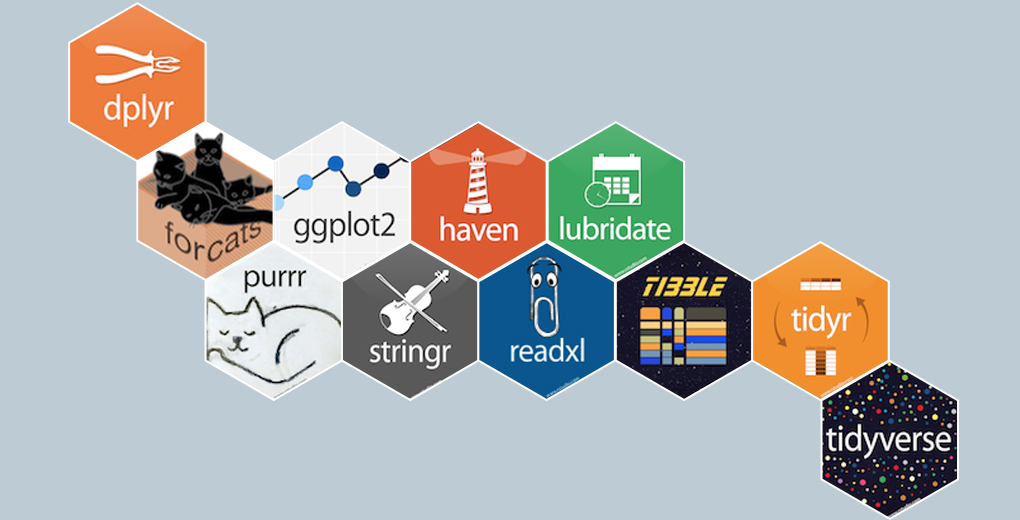
\includegraphics{images/tidyverse.png}

The Tidyverse is a comprehensive ecosystem of R packages that share common principles for data manipulation and visualization. It encourages the use of tidy data, a specific data structure that makes data analysis more straightforward. Tidy data arranges observations in rows and variables in columns, making it easier to work with and visualize.

\hypertarget{key-tidyverse-packages}{%
\section{Key Tidyverse Packages}\label{key-tidyverse-packages}}

Let's dive into some of the essential packages within the Tidyverse and understand how they can be beneficial in data analysis.

\hypertarget{dplyr}{%
\subsection{dplyr}\label{dplyr}}

Explore dplyr docs \href{https://dplyr.tidyverse.org/}{here}.

The core of the Tidyverse is the \texttt{dplyr} package. It provides a set of functions for data manipulation, including filtering, summarizing, and transforming data frames. Here's a simple example of how you might use \texttt{dplyr} to filter data:

\begin{Shaded}
\begin{Highlighting}[]
\CommentTok{\# install.packages("dplyr")}
\CommentTok{\# Load the dplyr package}
\FunctionTok{library}\NormalTok{(dplyr)}

\CommentTok{\# Create a data frame}
\NormalTok{data }\OtherTok{\textless{}{-}} \FunctionTok{data.frame}\NormalTok{(}
  \AttributeTok{Name =} \FunctionTok{c}\NormalTok{(}\StringTok{"Alice"}\NormalTok{, }\StringTok{"Bob"}\NormalTok{, }\StringTok{"Charlie"}\NormalTok{),}
  \AttributeTok{Age =} \FunctionTok{c}\NormalTok{(}\DecValTok{25}\NormalTok{, }\DecValTok{30}\NormalTok{, }\DecValTok{22}\NormalTok{)}
\NormalTok{)}

\NormalTok{data }
\end{Highlighting}
\end{Shaded}

\begin{verbatim}
##      Name Age
## 1   Alice  25
## 2     Bob  30
## 3 Charlie  22
\end{verbatim}

\begin{Shaded}
\begin{Highlighting}[]
\CommentTok{\# Filter the data to select individuals older than 25}
\NormalTok{filtered\_data }\OtherTok{\textless{}{-}}\NormalTok{ data }\SpecialCharTok{\%\textgreater{}\%}
  \FunctionTok{filter}\NormalTok{(Age }\SpecialCharTok{\textgreater{}} \DecValTok{25}\NormalTok{)}

\CommentTok{\# View the filtered data}
\NormalTok{filtered\_data}
\end{Highlighting}
\end{Shaded}

\begin{verbatim}
##   Name Age
## 1  Bob  30
\end{verbatim}

In this example, we used \texttt{filter()} to select rows where the ``Age'' column is greater than 25.

\hypertarget{a-note-on-the-pipe}{%
\subsection{A note on the pipe}\label{a-note-on-the-pipe}}

You just saw the \texttt{\%\textgreater{}\%} operator. It is also called a pipe.

\texttt{\%\textgreater{}\%} is from the \href{https://cran.r-project.org/web/packages/magrittr/vignettes/magrittr.html}{magrittr} package and when you load the \texttt{dplyr} package, the \texttt{\%\textgreater{}\%} will be available for you to use.

The R language has a new, built-in pipe operator as of R version 4.1: \texttt{\textbar{}\textgreater{}}.

\begin{Shaded}
\begin{Highlighting}[]
\NormalTok{mtcars }\SpecialCharTok{\%\textgreater{}\%}
  \FunctionTok{head}\NormalTok{()}
\end{Highlighting}
\end{Shaded}

\begin{verbatim}
##                    mpg cyl disp  hp drat    wt  qsec vs am gear carb
## Mazda RX4         21.0   6  160 110 3.90 2.620 16.46  0  1    4    4
## Mazda RX4 Wag     21.0   6  160 110 3.90 2.875 17.02  0  1    4    4
## Datsun 710        22.8   4  108  93 3.85 2.320 18.61  1  1    4    1
## Hornet 4 Drive    21.4   6  258 110 3.08 3.215 19.44  1  0    3    1
## Hornet Sportabout 18.7   8  360 175 3.15 3.440 17.02  0  0    3    2
## Valiant           18.1   6  225 105 2.76 3.460 20.22  1  0    3    1
\end{verbatim}

\begin{Shaded}
\begin{Highlighting}[]
\NormalTok{mtcars }\SpecialCharTok{|\textgreater{}}
  \FunctionTok{head}\NormalTok{()}
\end{Highlighting}
\end{Shaded}

\begin{verbatim}
##                    mpg cyl disp  hp drat    wt  qsec vs am gear carb
## Mazda RX4         21.0   6  160 110 3.90 2.620 16.46  0  1    4    4
## Mazda RX4 Wag     21.0   6  160 110 3.90 2.875 17.02  0  1    4    4
## Datsun 710        22.8   4  108  93 3.85 2.320 18.61  1  1    4    1
## Hornet 4 Drive    21.4   6  258 110 3.08 3.215 19.44  1  0    3    1
## Hornet Sportabout 18.7   8  360 175 3.15 3.440 17.02  0  0    3    2
## Valiant           18.1   6  225 105 2.76 3.460 20.22  1  0    3    1
\end{verbatim}

Think of \texttt{\%\textgreater{}\%} and \texttt{\textbar{}\textgreater{}} in R the same as \texttt{\textbar{}} in the unix commands: the output of the previous command is the input of the next command.

The pipe operator \texttt{\%\textgreater{}\%} is a very useful tool for writing efficient, easy-to-read code in R. You can use as many pipes as you want. I usually build the pipes one by one by looking at the output.

\begin{Shaded}
\begin{Highlighting}[]
\NormalTok{mtcars }\SpecialCharTok{\%\textgreater{}\%} 
  \FunctionTok{head}\NormalTok{() }\SpecialCharTok{\%\textgreater{}\%} 
  \FunctionTok{tail}\NormalTok{(}\AttributeTok{n=}\DecValTok{3}\NormalTok{)}
\end{Highlighting}
\end{Shaded}

\begin{verbatim}
##                    mpg cyl disp  hp drat    wt  qsec vs am gear carb
## Hornet 4 Drive    21.4   6  258 110 3.08 3.215 19.44  1  0    3    1
## Hornet Sportabout 18.7   8  360 175 3.15 3.440 17.02  0  0    3    2
## Valiant           18.1   6  225 105 2.76 3.460 20.22  1  0    3    1
\end{verbatim}

This means print out the first 6 rows and then take the last 3 rows.

\hypertarget{ggplot2}{%
\subsection{ggplot2}\label{ggplot2}}

Explore \texttt{ggplot2} docs \href{https://ggplot2.tidyverse.org/index.html}{here}.

The \texttt{ggplot2} package is the go-to choice for data visualization in the Tidyverse. It follows the ``grammar of graphics'' approach, allowing you to build complex plots layer by layer. Here's a basic example:

\begin{Shaded}
\begin{Highlighting}[]
\CommentTok{\# install.packages("ggplot2")}
\CommentTok{\# Load the ggplot2 package}
\FunctionTok{library}\NormalTok{(ggplot2)}

\CommentTok{\# Create a scatter plot}
\FunctionTok{ggplot}\NormalTok{(data, }\FunctionTok{aes}\NormalTok{(}\AttributeTok{x =}\NormalTok{ Age, }\AttributeTok{y =}\NormalTok{ Name)) }\SpecialCharTok{+}
  \FunctionTok{geom\_point}\NormalTok{()}
\end{Highlighting}
\end{Shaded}

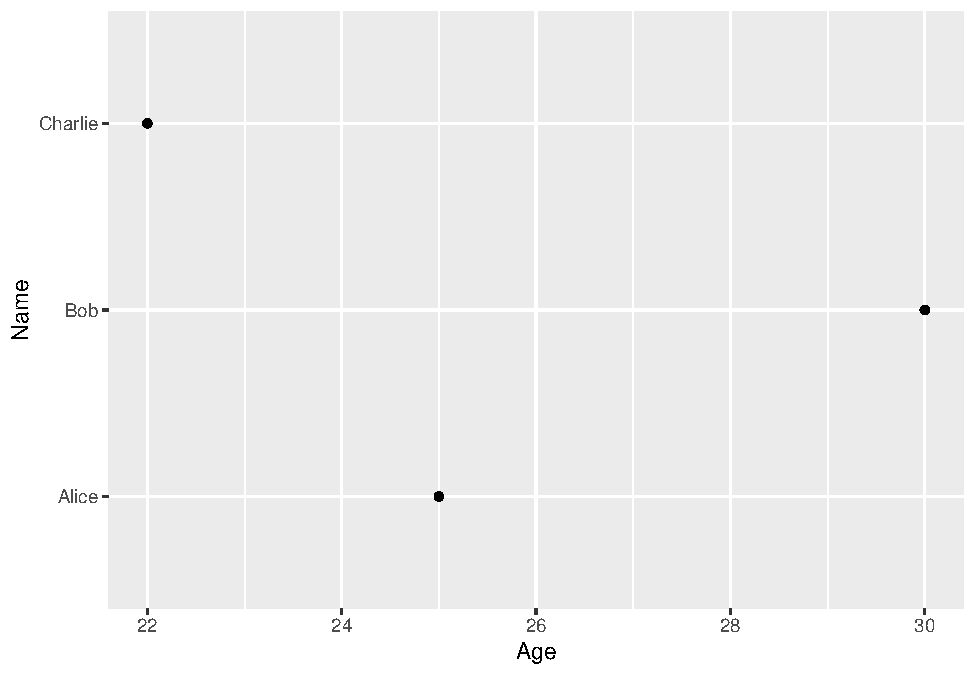
\includegraphics{08_Introduction_to_the_tidyverse_ecosystem_files/figure-latex/unnamed-chunk-4-1.pdf}

n this code, we used \texttt{ggplot()} to set up the plot and \texttt{geom\_point()} to add scatterplot points to the canvas.

\hypertarget{tidyr}{%
\subsection{tidyr}\label{tidyr}}

Explore tidyr docs \href{https://tidyr.tidyverse.org/index.html}{here}.

The \texttt{tidyr} package assists in reshaping data between \textbf{wide} and \textbf{long} formats, which is often necessary for analysis and visualization. Suppose you have a dataset with columns representing different years and want to convert it to a long format for easier analysis. \texttt{tidyr} can help with this transformation.

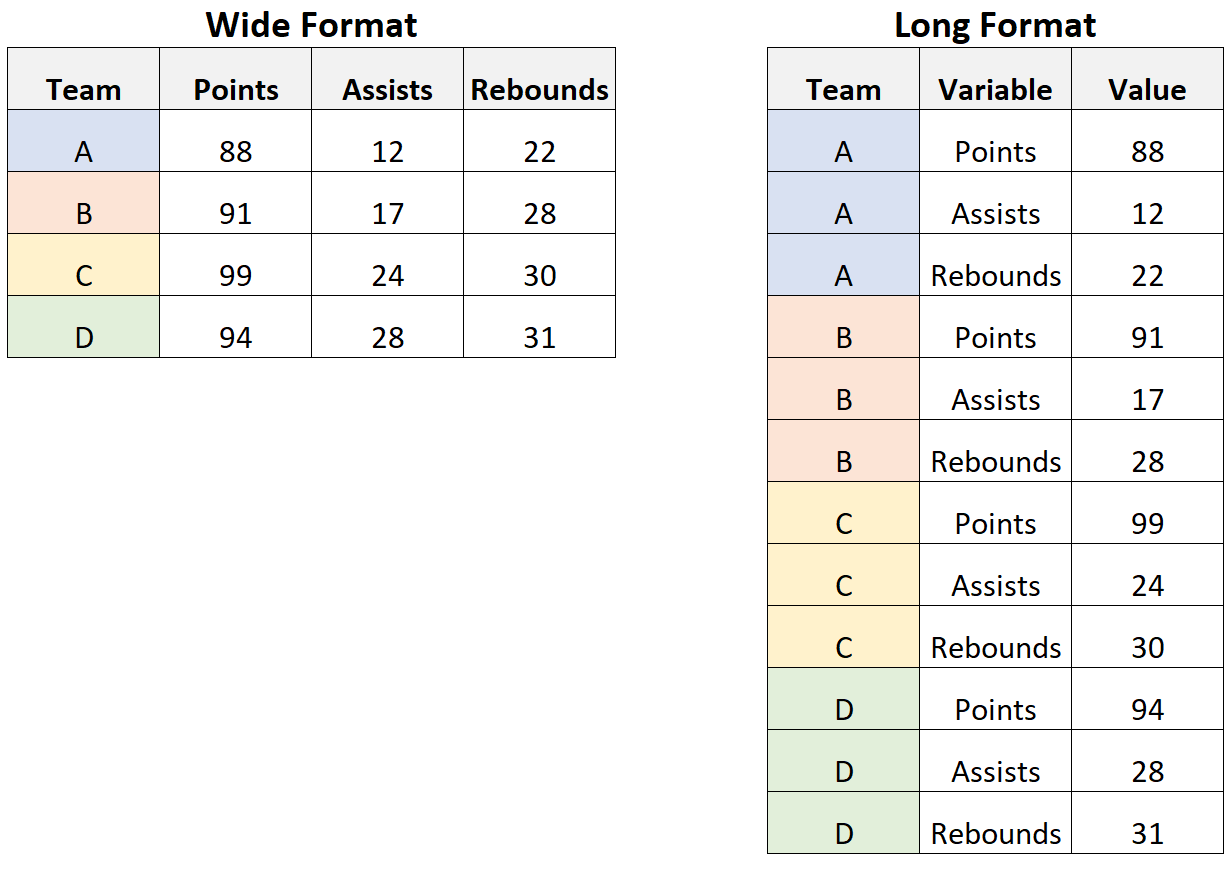
\includegraphics[width=1\linewidth]{images/wide}

\hypertarget{readr}{%
\subsection{readr}\label{readr}}

Explore readr docs \href{https://readr.tidyverse.org/index.html}{here}.

\texttt{readr} is a fast and efficient package for reading \textbf{tabular} data into R. It's faster than the base R functions like \texttt{read.csv()}. When working with large datasets, this can significantly speed up your data loading process.

Tabular data are rectangular:

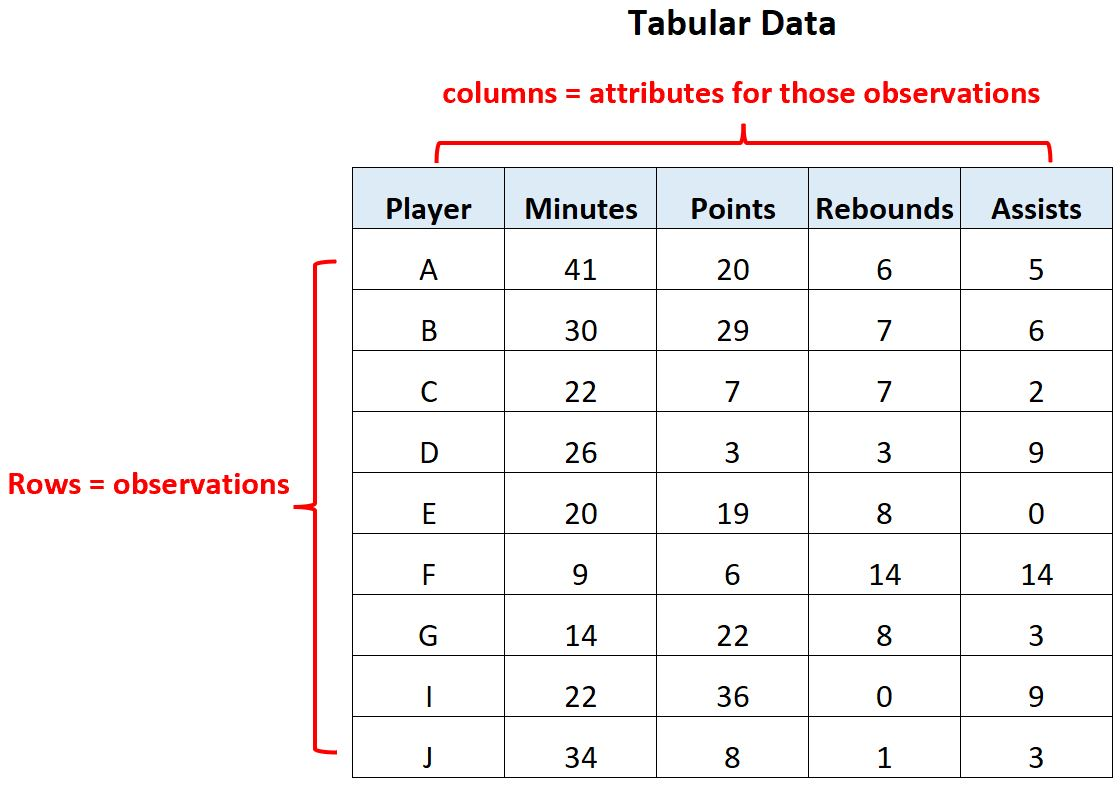
\includegraphics{images/tabular.jpeg}

\hypertarget{tibble}{%
\subsection{tibble}\label{tibble}}

Explore tibble docs \href{https://tibble.tidyverse.org/index.html}{here}.

the rectangular data will be read into R as a dataframe. \texttt{tibble} provides an improved data frame structure that addresses some issues with traditional R data frames. It displays data more neatly and provides better compatibility with the Tidyverse functions.

\hypertarget{stringr}{%
\subsection{stringr}\label{stringr}}

Explore stringr docs \href{https://stringr.tidyverse.org/index.html}{here}.

The \texttt{stringr} package offers a range of string manipulation functions that are easier to use and more consistent than the base R functions. It's particularly handy when dealing with text data, such as cleaning and formatting strings.

\hypertarget{forcats}{%
\subsection{forcats}\label{forcats}}

Explore forcats docs \href{https://forcats.tidyverse.org/index.html}{here}.

\texttt{forcats} is designed for handling factor variables, which are categorical variables with predefined levels. It provides tools for changing the order of levels and combining levels when necessary.

\hypertarget{real-world-applications-1}{%
\subsection{Real-World Applications}\label{real-world-applications-1}}

To illustrate the practical utility of the Tidyverse, consider the following scenarios:

\begin{enumerate}
\def\labelenumi{\arabic{enumi}.}
\item
  Data Import: \texttt{readr} helps you efficiently import data from various sources, such as CSV files, Excel spreadsheets, or even web-based data.
\item
  Data Cleaning: When working with messy data, \texttt{tidyr} and \texttt{stringr} can assist in reshaping and cleaning data for analysis.
\item
  Data Exploration: When you receive a dataset, you can use \texttt{dplyr} to quickly filter, summarize, and explore the data, helping you understand its characteristics.
\item
  Data Visualization: \texttt{ggplot2} allows you to create stunning visualizations, making it easier to convey insights to others. For instance, you can create bar charts, scatter plots, and histograms.
\item
  Working with Factors: \texttt{forcats} simplifies tasks like reordering factor levels for better visual representation.
\end{enumerate}

By mastering the Tidyverse, you'll have a powerful set of tools at your disposal for all stages of data analysis, from data preprocessing to visualization and modeling. Happy coding!

\hypertarget{tibble-and-readr---modern-data-structures-in-r}{%
\section{Tibble and Readr - Modern Data Structures in R}\label{tibble-and-readr---modern-data-structures-in-r}}

In this lesson, we will explore two essential concepts in data manipulation with R: tibbles and the readr package. These tools are designed to make working with data more efficient and user-friendly, especially when dealing with large datasets. We'll see why tibbles are preferred over traditional data frames and how to read and manipulate data using the readr package.

\hypertarget{tibbles-a-better-way-to-store-data}{%
\subsection{Tibbles: A Better Way to Store Data}\label{tibbles-a-better-way-to-store-data}}

Traditional Data Frames vs.~Tibbles:
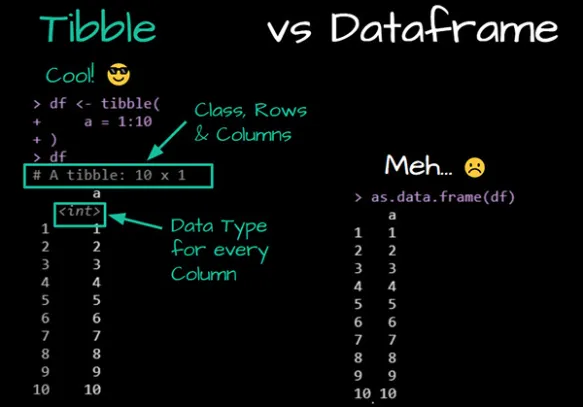
\includegraphics{images/tibble.png}

In R, data frames are widely used for storing and manipulating data. However, tibbles offer several advantages over traditional data frames:

\begin{enumerate}
\def\labelenumi{\arabic{enumi}.}
\item
  Cleaner Printing: Tibbles offer a more organized way to present your data. When you print a tibble, it only displays the first 10 rows and as many columns as can fit on your screen. This ensures a concise overview of your data, which is particularly helpful for large datasets. In contrast, traditional data frames tend to print all rows and columns by default, leading to overwhelming output.
\item
  Structured Indexing: When you subset a tibble using {[} {]}, it returns another tibble that retains the original data's structure. This means you still have clear column names and data types. In contrast, data frames return vectors, which provide less information about the structure of the data subset. You need to specify drop = FALSE to retain as a data frame and we see examples in previous lectures.
\item
  Preservation of Variable Types: Tibbles respect the original data types of your variables, even after subsetting. This is important because it ensures that your data remains consistent. In some cases, data frames may convert variables to factors or matrices when you subset them, potentially causing unexpected issues.
\item
  String Handling: In tibbles, character vectors remain as characters, maintaining the integrity of your data. However, data frames may automatically convert character vectors to factors by default. This behavior can lead to unexpected changes in your data and, subsequently, your analysis.
\item
  List-Columns: One unique feature of tibbles is their ability to directly contain list-columns. List-columns allow you to store lists within your tibble, providing a convenient way to work with complex data structures. Data frames do not offer this feature, which can limit your ability to represent certain types of data effectively.
\item
  Enhanced Output: Tibbles enhance the print display by showing data types, highlighting missing values, and truncating output for better readability. This additional information helps you understand your data at a glance, making it easier to spot potential issues or trends.
\end{enumerate}

\hypertarget{rownames-and-tibbles}{%
\subsection{Rownames and Tibbles}\label{rownames-and-tibbles}}

In regular data frames, you can assign and work with rownames, which are helpful for labeling and referencing rows. However, tibbles do not support rownames, so you want to add another column that contains the row ids.

\hypertarget{reading-data-with-readr}{%
\subsection{Reading Data with readr}\label{reading-data-with-readr}}

To work with data effectively, you first need to import it into R. The \texttt{readr} package provides a powerful toolset for reading various data file formats. Let's see how to read data using readr.

\hypertarget{reading-csv-data}{%
\subsubsection{Reading CSV Data}\label{reading-csv-data}}

Download the TCGA gene expression data (CSV file) to your working directory or specify the correct file path.

\begin{quote}
Download the file at \url{https://osf.io/yeun5}
\end{quote}

Click the \texttt{Download}:

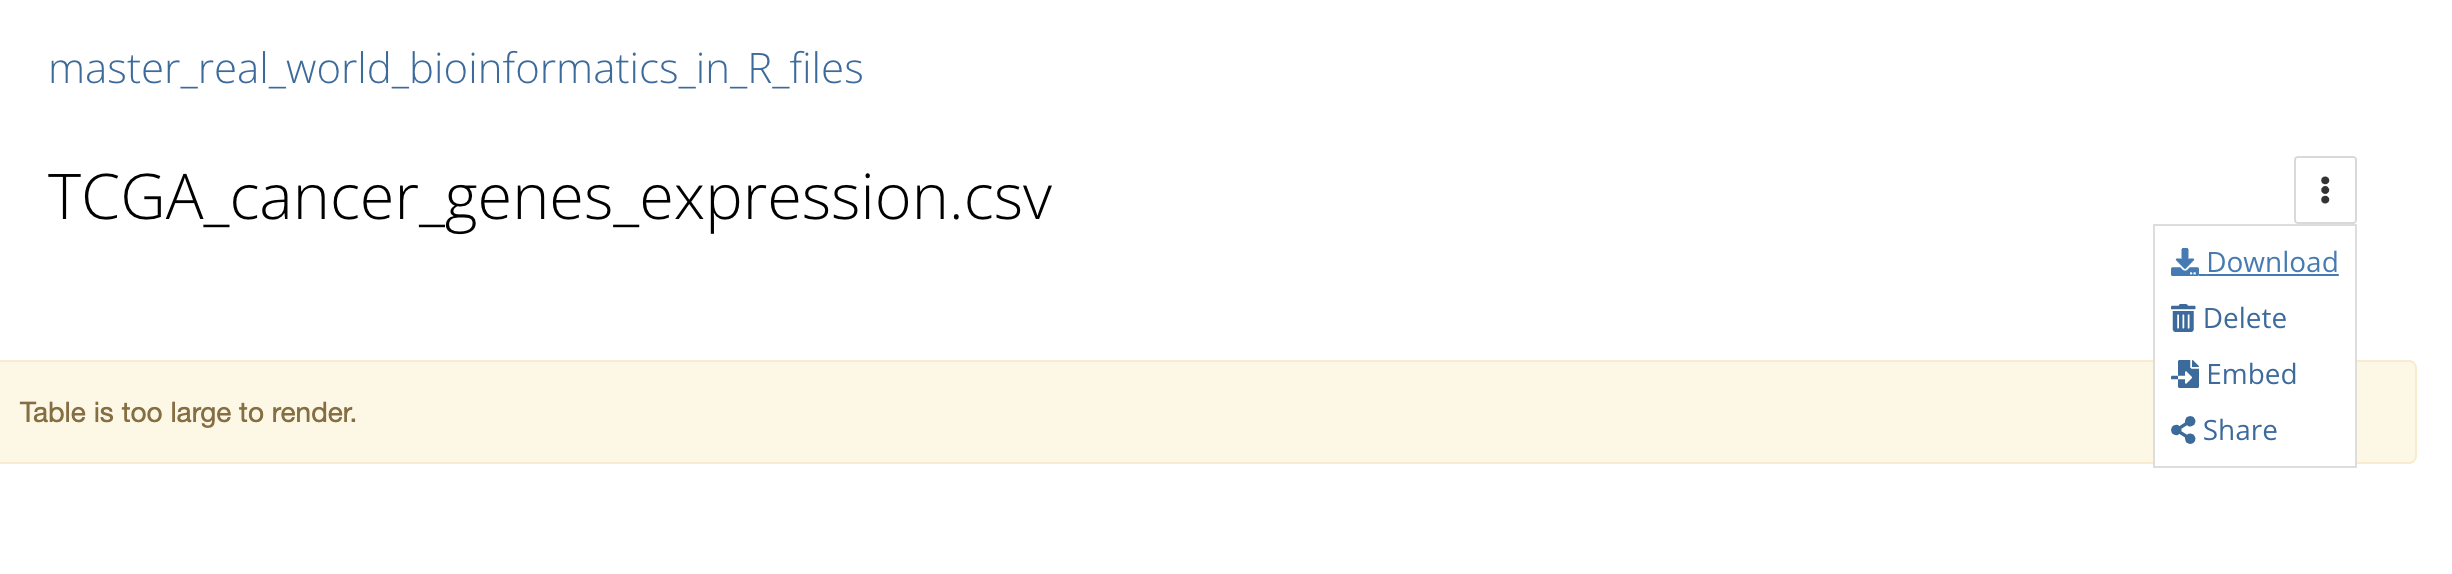
\includegraphics{images/osf.png}

Suppose we have a CSV file named ``TCGA\_cancer\_genes\_expression.csv'' in the Downloads folder, to read it using \texttt{readr::read\_csv}, follow these steps:

\begin{Shaded}
\begin{Highlighting}[]
\CommentTok{\# Load the readr package (if not already loaded)}
\FunctionTok{library}\NormalTok{(readr)}

\CommentTok{\# Read the CSV data into a tibble}
\NormalTok{tcga\_data }\OtherTok{\textless{}{-}}\NormalTok{ readr}\SpecialCharTok{::}\FunctionTok{read\_csv}\NormalTok{(}\StringTok{"\textasciitilde{}/Downloads/TCGA\_cancer\_genes\_expression.csv"}\NormalTok{)}

\CommentTok{\# Display the first few rows of the tibble}
\FunctionTok{head}\NormalTok{(tcga\_data)}
\end{Highlighting}
\end{Shaded}

\begin{verbatim}
## # A tibble: 6 x 25
##   ...1      TACSTD2  VTCN1   MUC1 NECTIN4 FOLH1  FOLR1 CD276   MSLN  CLDN6 ERBB2
##   <chr>       <dbl>  <dbl>  <dbl>   <dbl> <dbl>  <dbl> <dbl>  <dbl>  <dbl> <dbl>
## 1 43e715bf~   0.704 0      0.675   0.0862  7.21 0       52.8 0.0667 0.0970  1.88
## 2 1a5db9fc~  25.4   0      2.02    0.0728 23.6  0.122   78.8 0.956  0.255   7.78
## 3 93b382e4~   1.58  0      0.908   0.699   2.85 1.01   146.  0.0456 0.257   2.91
## 4 1f39dadd~   0.270 0.0910 0.0429  0.0165  1.16 0.279   48.5 0.0315 0.247   4.91
## 5 8c8c09b9~   0.412 0      0.115   0.0317  2.41 0.0492  42.3 0.270  0.126   1.49
## 6 85a86b91~   4.55  4.86   0.0421  0.0683  1.01 0.0225  20.6 0.0134 0.0182 13.5 
## # i 14 more variables: MUC16 <dbl>, DLL3 <dbl>, CEACAM5 <dbl>, PVR <dbl>,
## #   EPCAM <dbl>, PROM1 <dbl>, CD24 <dbl>, EGFR <dbl>, MET <dbl>,
## #   TNFRSF10B <dbl>, tcga.tcga_barcode <chr>,
## #   tcga.cgc_sample_sample_type <chr>, study <chr>, sample_type <chr>
\end{verbatim}

Here, we load the \texttt{readr} package, use \texttt{read\_csv} to read the CSV file, and store the data in the \texttt{tcga\_data} tibble. Finally, we use \texttt{head} to display the first few rows of the tibble.

note that the first column's name changes to ``\ldots1,'' which is a default behavior when column names are missing in the source data.

\hypertarget{understanding-the-output}{%
\subsubsection{Understanding the Output}\label{understanding-the-output}}

The output shows the data in a neat tabular format. Column names are displayed at the top, followed by rows of data. Each column's data type is indicated (e.g., \texttt{dbl} for double-precision floating point numbers or \texttt{chr} for character).

\hypertarget{using-tibbles-with-imported-data}{%
\subsection{Using Tibbles with Imported Data}\label{using-tibbles-with-imported-data}}

When working with tibbles, imported data maintains its format and advantages over data frames. Here's how you can convert the imported data into a tibble:

\begin{Shaded}
\begin{Highlighting}[]
\CommentTok{\# Load the dplyr package for tibble conversion}
\FunctionTok{library}\NormalTok{(dplyr)}

\CommentTok{\# read in the data using built{-}in read.csv}
\NormalTok{tcga\_data}\OtherTok{\textless{}{-}} \FunctionTok{read.csv}\NormalTok{(}\StringTok{"\textasciitilde{}/Downloads/TCGA\_cancer\_genes\_expression.csv"}\NormalTok{)}

\CommentTok{\# regular dataframe, and the first column name is X if it is empty}
\FunctionTok{head}\NormalTok{(tcga\_data)}
\end{Highlighting}
\end{Shaded}

\begin{verbatim}
##                                      X    TACSTD2      VTCN1       MUC1
## 1 43e715bf-28d9-4b5e-b762-8cd1b69a430e  0.7035937 0.00000000 0.67502205
## 2 1a5db9fc-2abd-4e1b-b5ef-b1cf5e5f3872 25.4360736 0.00000000 2.01525394
## 3 93b382e4-9c9a-43f5-bd3b-502cc260b886  1.5756197 0.00000000 0.90784666
## 4 1f39dadd-3655-474e-ba4c-a5bd32c97a8b  0.2702156 0.09099681 0.04293345
## 5 8c8c09b9-ec83-45ec-bc4c-0ba92de60acb  0.4122814 0.00000000 0.11484380
## 6 85a86b91-4f24-4e77-ae2d-520f8e205efc  4.5469193 4.85973690 0.04208195
##      NECTIN4     FOLH1      FOLR1     CD276       MSLN      CLDN6     ERBB2
## 1 0.08620727  7.213342 0.00000000  52.75981 0.06674445 0.09704962  1.879518
## 2 0.07279804 23.552286 0.12154673  78.78551 0.95554610 0.25458796  7.777976
## 3 0.69905270  2.853812 1.01000271 145.84399 0.04563568 0.25701910  2.905926
## 4 0.01652257  1.157070 0.27942068  48.45022 0.03154912 0.24746913  4.914280
## 5 0.03168398  2.408137 0.04922458  42.25592 0.26968788 0.12576720  1.494744
## 6 0.06828305  1.010411 0.02248965  20.63795 0.01336404 0.01823883 13.474689
##          MUC16       DLL3 CEACAM5      PVR     EPCAM       PROM1       CD24
## 1 0.0011479879 0.49589978       0 52.08113  4.521984 0.025311008 0.55036003
## 2 0.0008049670 2.52244014       0 40.87926  9.530414 0.023576862 9.67272890
## 3 0.0026190288 0.77074712       0 33.26727 42.358567 0.000000000 0.06939934
## 4 0.0051705741 0.10636402       0 28.26457 16.316524 0.007783431 0.84522244
## 5 0.0004894306 0.04483123       0 41.66776 12.529742 0.019204339 0.21369023
## 6 0.0000000000 0.01184285       0 30.18711  2.430109 0.043719865 4.95506593
##        EGFR        MET TNFRSF10B            tcga.tcga_barcode
## 1  1.286481  0.9320235  12.80547 TCGA-OR-A5KU-01A-11R-A29S-07
## 2  5.373307  8.0610999  31.46289 TCGA-P6-A5OG-01A-22R-A29S-07
## 3  4.600918  0.1295387  65.57967 TCGA-OR-A5K5-01A-11R-A29S-07
## 4  3.010374  2.9728030  24.31636 TCGA-OR-A5K4-01A-11R-A29S-07
## 5 16.476552 19.7360055  21.11014 TCGA-OR-A5LP-01A-11R-A29S-07
## 6  2.010338  8.6087283  37.91574 TCGA-PK-A5H9-01A-11R-A29S-07
##   tcga.cgc_sample_sample_type study sample_type
## 1               Primary Tumor   ACC      cancer
## 2               Primary Tumor   ACC      cancer
## 3               Primary Tumor   ACC      cancer
## 4               Primary Tumor   ACC      cancer
## 5               Primary Tumor   ACC      cancer
## 6               Primary Tumor   ACC      cancer
\end{verbatim}

\begin{Shaded}
\begin{Highlighting}[]
\CommentTok{\# Convert the data to a tibble}
\NormalTok{tcga\_data }\OtherTok{\textless{}{-}}\NormalTok{ tcga\_data }\SpecialCharTok{\%\textgreater{}\%} 
\NormalTok{  tibble}\SpecialCharTok{::}\FunctionTok{as\_tibble}\NormalTok{()}

\CommentTok{\# Display the first few rows of the tibble}
\FunctionTok{head}\NormalTok{(tcga\_data)}
\end{Highlighting}
\end{Shaded}

\begin{verbatim}
## # A tibble: 6 x 25
##   X         TACSTD2  VTCN1   MUC1 NECTIN4 FOLH1  FOLR1 CD276   MSLN  CLDN6 ERBB2
##   <chr>       <dbl>  <dbl>  <dbl>   <dbl> <dbl>  <dbl> <dbl>  <dbl>  <dbl> <dbl>
## 1 43e715bf~   0.704 0      0.675   0.0862  7.21 0       52.8 0.0667 0.0970  1.88
## 2 1a5db9fc~  25.4   0      2.02    0.0728 23.6  0.122   78.8 0.956  0.255   7.78
## 3 93b382e4~   1.58  0      0.908   0.699   2.85 1.01   146.  0.0456 0.257   2.91
## 4 1f39dadd~   0.270 0.0910 0.0429  0.0165  1.16 0.279   48.5 0.0315 0.247   4.91
## 5 8c8c09b9~   0.412 0      0.115   0.0317  2.41 0.0492  42.3 0.270  0.126   1.49
## 6 85a86b91~   4.55  4.86   0.0421  0.0683  1.01 0.0225  20.6 0.0134 0.0182 13.5 
## # i 14 more variables: MUC16 <dbl>, DLL3 <dbl>, CEACAM5 <dbl>, PVR <dbl>,
## #   EPCAM <dbl>, PROM1 <dbl>, CD24 <dbl>, EGFR <dbl>, MET <dbl>,
## #   TNFRSF10B <dbl>, tcga.tcga_barcode <chr>,
## #   tcga.cgc_sample_sample_type <chr>, study <chr>, sample_type <chr>
\end{verbatim}

By using the \texttt{\%\textgreater{}\%} pipe operator and \texttt{tibble::as\_tibble()}, we convert the data into a tibble while preserving its structure and advantages.

The output remains in a similar format as before, with clear column names and data types.

\hypertarget{note-on-reading-excel-files}{%
\subsection{Note on reading Excel files}\label{note-on-reading-excel-files}}

We still deal with a lot of spreadsheets, to read in Excel files, take a look at the \href{https://readxl.tidyverse.org/}{\texttt{readxl}} package.

\hypertarget{conclusion-18}{%
\subsection{Conclusion}\label{conclusion-18}}

In this lesson, we learned about \texttt{tibbles}, a modern data structure in R that offers several advantages over traditional data frames. We also explored how to read and manipulate data using the readr package, converting imported data into tibbles for efficient data analysis. Tibbles and readr are valuable tools for data scientists and analysts working with R, making data manipulation and exploration more user-friendly and efficient.

\hypertarget{the-tidy-data-format}{%
\section{The tidy data format}\label{the-tidy-data-format}}

In this lesson, we will delve into the essential data cleaning and tidying operations in R using the powerful dplyr package. Tidying data is a crucial step in data analysis, especially when dealing with real-world data that can be messy and inconsistent. We will explore the concept of tidy data and learn about the distinction between long and wide dataset formats.

\hypertarget{the-importance-of-tidy-data}{%
\subsection{The Importance of Tidy Data}\label{the-importance-of-tidy-data}}

Real-world data is often messy, scattered across various files, missing metadata, and inputted in inconsistent formats. Before we can effectively analyze this data, we need to bring it all together into one structured table and resolve any issues. This process of data ingestion and standardization is known as data tidying.

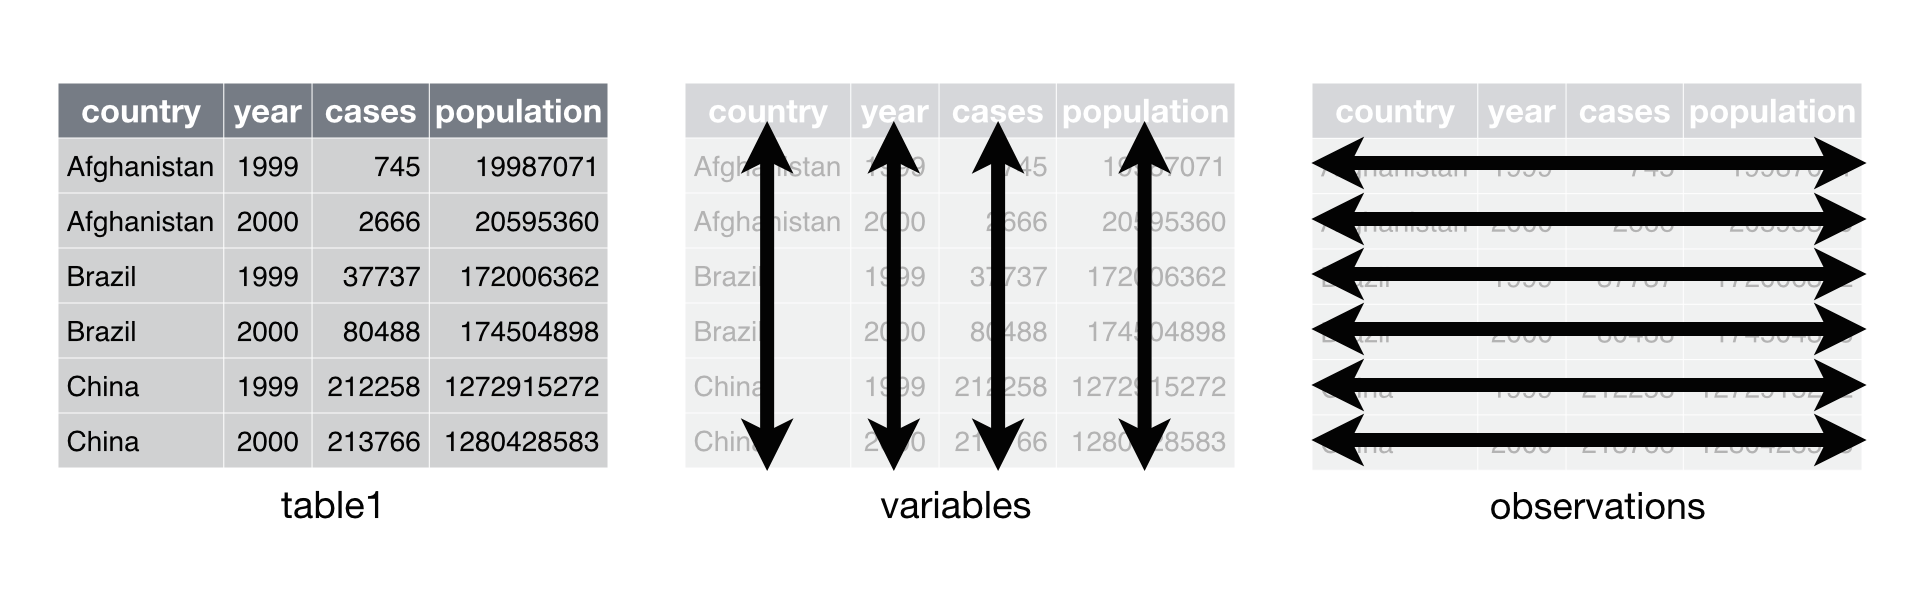
\includegraphics{images/tidy-data.png}

The tidyverse packages, including \texttt{dplyr}, work seamlessly with tidy data. As defined by Hadley Wickham in \href{https://r4ds.had.co.nz/}{R for Data Science}, tidy data adheres to three interrelated rules:

\begin{enumerate}
\def\labelenumi{\arabic{enumi}.}
\item
  Each variable must have its own column.
\item
  Each observation must have its own row.
\item
  Each value must have its own cell.
\end{enumerate}

Why should we make our data tidy? There are both general and specific advantages:

\begin{itemize}
\item
  General Advantage: Using a consistent data structure makes it easier to learn and work with data manipulation tools because they follow a uniform pattern.
\item
  Specific Advantage: Placing variables in columns allows R's vectorized nature to shine. Most built-in R functions work efficiently with vectors of values. This natural alignment between tidy data and R's capabilities makes data transformation feel particularly intuitive.
\end{itemize}

\hypertarget{long-format-vs.-wide-format}{%
\subsection{Long Format vs.~Wide Format}\label{long-format-vs.-wide-format}}

Before we dive into the practical aspects of tidying data, let's understand the difference between long format and wide format for a dataframe. We'll use an example with the dplyr package:

\begin{Shaded}
\begin{Highlighting}[]
\FunctionTok{library}\NormalTok{(tidyverse)}

\FunctionTok{head}\NormalTok{(table4a)}
\end{Highlighting}
\end{Shaded}

\begin{verbatim}
## # A tibble: 3 x 3
##   country     `1999` `2000`
##   <chr>        <dbl>  <dbl>
## 1 Afghanistan    745   2666
## 2 Brazil       37737  80488
## 3 China       212258 213766
\end{verbatim}

The \texttt{table4a} dataframe is in the wide format, which is a common way to enter data into software like Excel. In this format, each column often represents a year, and the values are spread across columns for each country.

To convert this data into the long format, we'll use \texttt{tidyr::pivot\_longer()}. This function reshapes the data, making it easier to work with:

\begin{Shaded}
\begin{Highlighting}[]
\NormalTok{table4a }\SpecialCharTok{\%\textgreater{}\%} 
  \FunctionTok{pivot\_longer}\NormalTok{(}\FunctionTok{c}\NormalTok{(}\StringTok{\textasciigrave{}}\AttributeTok{1999}\StringTok{\textasciigrave{}}\NormalTok{, }\StringTok{\textasciigrave{}}\AttributeTok{2000}\StringTok{\textasciigrave{}}\NormalTok{), }\AttributeTok{names\_to =} \StringTok{"year"}\NormalTok{, }\AttributeTok{values\_to =} \StringTok{"cases"}\NormalTok{)}
\end{Highlighting}
\end{Shaded}

\begin{verbatim}
## # A tibble: 6 x 3
##   country     year   cases
##   <chr>       <chr>  <dbl>
## 1 Afghanistan 1999     745
## 2 Afghanistan 2000    2666
## 3 Brazil      1999   37737
## 4 Brazil      2000   80488
## 5 China       1999  212258
## 6 China       2000  213766
\end{verbatim}

Now, the data fulfills the three rules for tidy data:

\begin{enumerate}
\def\labelenumi{\arabic{enumi}.}
\item
  Each variable (country and year) has its own column.
\item
  Each observation (combinations of country and year) has its own row.
\item
  Each value (the number of cases) has its own cell.
\end{enumerate}

Understanding the difference between long and wide formats is essential because it determines how we structure our data for analysis. Once you grasp these concepts, reshaping and tidying data becomes a more comfortable and intuitive process.

Take your time to study and understand these data formats. It will significantly boost your confidence in reshaping and tidying data for your analytical tasks.

\hypertarget{introducing-dplyr-your-data-wrangling-toolkit}{%
\section{Introducing dplyr: Your Data Wrangling Toolkit}\label{introducing-dplyr-your-data-wrangling-toolkit}}

In this lesson, we'll delve into the world of the dplyr package in R, which offers a powerful and concise set of tools for working with data frames. As a biology student new to programming, dplyr will be your trusty companion for effortlessly managing, filtering, and summarizing biological data.

To master dplyr, it's crucial to grasp its five core functions: \texttt{mutate()}, \texttt{select()}, \texttt{filter()}, \texttt{summarise()}, and \texttt{arrange()}. Each function serves a specific purpose in data manipulation.

\hypertarget{selecting-specific-columns}{%
\subsection{Selecting Specific Columns}\label{selecting-specific-columns}}

We will be working with the same tibble called tcga\_data that has numerous columns, but you're interested in extracting the ``EPCAM'' column along with other metadata columns. \texttt{EPCAM}, short for epithelial cellular adhesion molecule, is highly relevant in the context of epithelial cancer cells.

\begin{Shaded}
\begin{Highlighting}[]
\NormalTok{tcga\_data }\SpecialCharTok{\%\textgreater{}\%}
  \FunctionTok{select}\NormalTok{(EPCAM, tcga.tcga\_barcode}\SpecialCharTok{:}\NormalTok{sample\_type)}
\end{Highlighting}
\end{Shaded}

\begin{verbatim}
## # A tibble: 11,348 x 5
##    EPCAM tcga.tcga_barcode            tcga.cgc_sample_sample~1 study sample_type
##    <dbl> <chr>                        <chr>                    <chr> <chr>      
##  1  4.52 TCGA-OR-A5KU-01A-11R-A29S-07 Primary Tumor            ACC   cancer     
##  2  9.53 TCGA-P6-A5OG-01A-22R-A29S-07 Primary Tumor            ACC   cancer     
##  3 42.4  TCGA-OR-A5K5-01A-11R-A29S-07 Primary Tumor            ACC   cancer     
##  4 16.3  TCGA-OR-A5K4-01A-11R-A29S-07 Primary Tumor            ACC   cancer     
##  5 12.5  TCGA-OR-A5LP-01A-11R-A29S-07 Primary Tumor            ACC   cancer     
##  6  2.43 TCGA-PK-A5H9-01A-11R-A29S-07 Primary Tumor            ACC   cancer     
##  7  3.74 TCGA-OR-A5LD-01A-11R-A29S-07 Primary Tumor            ACC   cancer     
##  8  4.08 TCGA-OR-A5JX-01A-11R-A29S-07 Primary Tumor            ACC   cancer     
##  9  2.84 TCGA-PK-A5H8-01A-11R-A29S-07 Primary Tumor            ACC   cancer     
## 10  3.61 TCGA-OR-A5J3-01A-11R-A29S-07 Primary Tumor            ACC   cancer     
## # i 11,338 more rows
## # i abbreviated name: 1: tcga.cgc_sample_sample_type
\end{verbatim}

This code utilizes the \texttt{select()} function to pick specific columns by their names, creating a tidy subset of your data. We used \texttt{:} to select a range of columns. Note that the columns are reordered
putting \texttt{EPCAM} to the first column.

You can also use index to select the columns

\begin{Shaded}
\begin{Highlighting}[]
\FunctionTok{colnames}\NormalTok{(tcga\_data)}
\end{Highlighting}
\end{Shaded}

\begin{verbatim}
##  [1] "X"                           "TACSTD2"                    
##  [3] "VTCN1"                       "MUC1"                       
##  [5] "NECTIN4"                     "FOLH1"                      
##  [7] "FOLR1"                       "CD276"                      
##  [9] "MSLN"                        "CLDN6"                      
## [11] "ERBB2"                       "MUC16"                      
## [13] "DLL3"                        "CEACAM5"                    
## [15] "PVR"                         "EPCAM"                      
## [17] "PROM1"                       "CD24"                       
## [19] "EGFR"                        "MET"                        
## [21] "TNFRSF10B"                   "tcga.tcga_barcode"          
## [23] "tcga.cgc_sample_sample_type" "study"                      
## [25] "sample_type"
\end{verbatim}

The \texttt{EPCAM} column is the 16th column; \texttt{tcga.tcga\_barcode} is the 23rd column;
\texttt{sample\_type} is 25th column:

\begin{Shaded}
\begin{Highlighting}[]
\NormalTok{tcga\_data }\SpecialCharTok{\%\textgreater{}\%}
  \FunctionTok{select}\NormalTok{(}\DecValTok{16}\NormalTok{, }\DecValTok{23}\SpecialCharTok{:}\DecValTok{25}\NormalTok{)}
\end{Highlighting}
\end{Shaded}

\begin{verbatim}
## # A tibble: 11,348 x 4
##    EPCAM tcga.cgc_sample_sample_type study sample_type
##    <dbl> <chr>                       <chr> <chr>      
##  1  4.52 Primary Tumor               ACC   cancer     
##  2  9.53 Primary Tumor               ACC   cancer     
##  3 42.4  Primary Tumor               ACC   cancer     
##  4 16.3  Primary Tumor               ACC   cancer     
##  5 12.5  Primary Tumor               ACC   cancer     
##  6  2.43 Primary Tumor               ACC   cancer     
##  7  3.74 Primary Tumor               ACC   cancer     
##  8  4.08 Primary Tumor               ACC   cancer     
##  9  2.84 Primary Tumor               ACC   cancer     
## 10  3.61 Primary Tumor               ACC   cancer     
## # i 11,338 more rows
\end{verbatim}

We can even mix the index with column names:

\begin{Shaded}
\begin{Highlighting}[]
\NormalTok{tcga\_data }\SpecialCharTok{\%\textgreater{}\%}
  \FunctionTok{select}\NormalTok{(EPCAM, }\DecValTok{23}\SpecialCharTok{:}\DecValTok{25}\NormalTok{)}
\end{Highlighting}
\end{Shaded}

\begin{verbatim}
## # A tibble: 11,348 x 4
##    EPCAM tcga.cgc_sample_sample_type study sample_type
##    <dbl> <chr>                       <chr> <chr>      
##  1  4.52 Primary Tumor               ACC   cancer     
##  2  9.53 Primary Tumor               ACC   cancer     
##  3 42.4  Primary Tumor               ACC   cancer     
##  4 16.3  Primary Tumor               ACC   cancer     
##  5 12.5  Primary Tumor               ACC   cancer     
##  6  2.43 Primary Tumor               ACC   cancer     
##  7  3.74 Primary Tumor               ACC   cancer     
##  8  4.08 Primary Tumor               ACC   cancer     
##  9  2.84 Primary Tumor               ACC   cancer     
## 10  3.61 Primary Tumor               ACC   cancer     
## # i 11,338 more rows
\end{verbatim}

\begin{Shaded}
\begin{Highlighting}[]
\CommentTok{\# save it to a new variable}

\NormalTok{tcga\_data}\OtherTok{\textless{}{-}}\NormalTok{ tcga\_data }\SpecialCharTok{\%\textgreater{}\%}
  \FunctionTok{select}\NormalTok{(EPCAM, }\DecValTok{23}\SpecialCharTok{:}\DecValTok{25}\NormalTok{)}
\end{Highlighting}
\end{Shaded}

\hypertarget{adding-new-columns}{%
\subsection{Adding New Columns}\label{adding-new-columns}}

The \texttt{mutate()} function allows you to introduce new variables that are derived from existing ones. For instance, you can create a new column, ``log2EPCAM,'' containing the logarithm base-2 of the EPCAM values:

\begin{Shaded}
\begin{Highlighting}[]
\NormalTok{tcga\_data}\OtherTok{\textless{}{-}}\NormalTok{ tcga\_data }\SpecialCharTok{\%\textgreater{}\%}
  \FunctionTok{mutate}\NormalTok{(}\AttributeTok{log2EPCAM =} \FunctionTok{log2}\NormalTok{(EPCAM))}

\NormalTok{tcga\_data}
\end{Highlighting}
\end{Shaded}

\begin{verbatim}
## # A tibble: 11,348 x 5
##    EPCAM tcga.cgc_sample_sample_type study sample_type log2EPCAM
##    <dbl> <chr>                       <chr> <chr>           <dbl>
##  1  4.52 Primary Tumor               ACC   cancer           2.18
##  2  9.53 Primary Tumor               ACC   cancer           3.25
##  3 42.4  Primary Tumor               ACC   cancer           5.40
##  4 16.3  Primary Tumor               ACC   cancer           4.03
##  5 12.5  Primary Tumor               ACC   cancer           3.65
##  6  2.43 Primary Tumor               ACC   cancer           1.28
##  7  3.74 Primary Tumor               ACC   cancer           1.90
##  8  4.08 Primary Tumor               ACC   cancer           2.03
##  9  2.84 Primary Tumor               ACC   cancer           1.51
## 10  3.61 Primary Tumor               ACC   cancer           1.85
## # i 11,338 more rows
\end{verbatim}

\hypertarget{reordering-columns}{%
\subsection{Reordering Columns}\label{reordering-columns}}

If you want to rearrange the order of columns, you can again use \texttt{select()}. Here, we move the ``log2EPCAM'' column to the front while keeping all other columns intact:

\begin{Shaded}
\begin{Highlighting}[]
\NormalTok{tcga\_data }\SpecialCharTok{\%\textgreater{}\%}
  \FunctionTok{select}\NormalTok{(EPCAM, log2EPCAM, }\FunctionTok{everything}\NormalTok{())}
\end{Highlighting}
\end{Shaded}

\begin{verbatim}
## # A tibble: 11,348 x 5
##    EPCAM log2EPCAM tcga.cgc_sample_sample_type study sample_type
##    <dbl>     <dbl> <chr>                       <chr> <chr>      
##  1  4.52      2.18 Primary Tumor               ACC   cancer     
##  2  9.53      3.25 Primary Tumor               ACC   cancer     
##  3 42.4       5.40 Primary Tumor               ACC   cancer     
##  4 16.3       4.03 Primary Tumor               ACC   cancer     
##  5 12.5       3.65 Primary Tumor               ACC   cancer     
##  6  2.43      1.28 Primary Tumor               ACC   cancer     
##  7  3.74      1.90 Primary Tumor               ACC   cancer     
##  8  4.08      2.03 Primary Tumor               ACC   cancer     
##  9  2.84      1.51 Primary Tumor               ACC   cancer     
## 10  3.61      1.85 Primary Tumor               ACC   cancer     
## # i 11,338 more rows
\end{verbatim}

The \texttt{everything()} helper function denotes all other columns, ensuring your numeric columns are at the front.

\hypertarget{filtering-data}{%
\subsection{Filtering Data}\label{filtering-data}}

\texttt{filter()} is your go-to function for extracting observations that meet specific criteria. To isolate data only related to glioblastoma (GBM), you can apply the following filter:

\begin{Shaded}
\begin{Highlighting}[]
\NormalTok{tcga\_data }\SpecialCharTok{\%\textgreater{}\%}
  \FunctionTok{filter}\NormalTok{(study }\SpecialCharTok{==} \StringTok{"GBM"}\NormalTok{)}
\end{Highlighting}
\end{Shaded}

\begin{verbatim}
## # A tibble: 175 x 5
##     EPCAM tcga.cgc_sample_sample_type study sample_type log2EPCAM
##     <dbl> <chr>                       <chr> <chr>           <dbl>
##  1 0.329  Primary Tumor               GBM   cancer         -1.60 
##  2 0.152  Primary Tumor               GBM   cancer         -2.72 
##  3 0.0814 Primary Tumor               GBM   cancer         -3.62 
##  4 0.367  Recurrent Tumor             GBM   cancer         -1.45 
##  5 0.0614 Primary Tumor               GBM   cancer         -4.02 
##  6 0.350  Primary Tumor               GBM   cancer         -1.51 
##  7 0.165  Primary Tumor               GBM   cancer         -2.60 
##  8 0.0989 Primary Tumor               GBM   cancer         -3.34 
##  9 0.466  Primary Tumor               GBM   cancer         -1.10 
## 10 0.707  Recurrent Tumor             GBM   cancer         -0.500
## # i 165 more rows
\end{verbatim}

This code snippet retains only the rows corresponding to GBM in your dataset.

\hypertarget{summarizing-data}{%
\subsection{Summarizing Data}\label{summarizing-data}}

Suppose you want to calculate the average EPCAM expression for each cancer type in your dataset. You can utilize \texttt{summarise()} in conjunction with \texttt{group\_by()}:

\begin{Shaded}
\begin{Highlighting}[]
\NormalTok{tcga\_data }\SpecialCharTok{\%\textgreater{}\%}
  \FunctionTok{group\_by}\NormalTok{(study) }\SpecialCharTok{\%\textgreater{}\%}
  \FunctionTok{summarise}\NormalTok{(}\AttributeTok{average\_EPCAM =} \FunctionTok{mean}\NormalTok{(EPCAM))}
\end{Highlighting}
\end{Shaded}

\begin{verbatim}
## # A tibble: 33 x 2
##    study average_EPCAM
##    <chr>         <dbl>
##  1 ACC          11.2  
##  2 BLCA        102.   
##  3 BRCA        177.   
##  4 CESC        166.   
##  5 CHOL        223.   
##  6 COAD        792.   
##  7 DLBC          2.61 
##  8 ESCA        273.   
##  9 GBM           0.623
## 10 HNSC         50.3  
## # i 23 more rows
\end{verbatim}

Here, the data is grouped by the ``study'' variable, and the \texttt{summarise()} function calculates the mean \texttt{EPCAM} value for each group.

\hypertarget{sorting-data}{%
\subsection{Sorting Data}\label{sorting-data}}

To sort your data frame based on a specific column, employ \texttt{arrange()}. For instance, you can order your dataset by the median level of EPCAM:

\begin{Shaded}
\begin{Highlighting}[]
\NormalTok{tcga\_data }\SpecialCharTok{\%\textgreater{}\%}
  \FunctionTok{group\_by}\NormalTok{(study) }\SpecialCharTok{\%\textgreater{}\%}
  \FunctionTok{summarise}\NormalTok{(}\AttributeTok{average\_EPCAM =} \FunctionTok{mean}\NormalTok{(EPCAM),}
            \AttributeTok{median\_EPCAM =} \FunctionTok{median}\NormalTok{(EPCAM)) }\SpecialCharTok{\%\textgreater{}\%}
  \FunctionTok{arrange}\NormalTok{(median\_EPCAM)}
\end{Highlighting}
\end{Shaded}

\begin{verbatim}
## # A tibble: 33 x 3
##    study average_EPCAM median_EPCAM
##    <chr>         <dbl>        <dbl>
##  1 UVM           0.765       0.0583
##  2 SKCM          0.980       0.133 
##  3 SARC          2.87        0.224 
##  4 GBM           0.623       0.323 
##  5 DLBC          2.61        0.578 
##  6 LAML          3.14        0.595 
##  7 LGG           0.906       0.681 
##  8 MESO         11.3         1.14  
##  9 LIHC         31.2         1.22  
## 10 ACC          11.2         4.83  
## # i 23 more rows
\end{verbatim}

The default is arrange from the smallest to the biggest. Let's reverse it by using the helper descending function \texttt{desc}:

\begin{Shaded}
\begin{Highlighting}[]
\NormalTok{tcga\_data }\SpecialCharTok{\%\textgreater{}\%}
  \FunctionTok{group\_by}\NormalTok{(study) }\SpecialCharTok{\%\textgreater{}\%}
  \FunctionTok{summarise}\NormalTok{(}\AttributeTok{average\_EPCAM =} \FunctionTok{mean}\NormalTok{(EPCAM),}
            \AttributeTok{median\_EPCAM =} \FunctionTok{median}\NormalTok{(EPCAM)) }\SpecialCharTok{\%\textgreater{}\%}
  \FunctionTok{arrange}\NormalTok{(}\FunctionTok{desc}\NormalTok{(median\_EPCAM))}
\end{Highlighting}
\end{Shaded}

\begin{verbatim}
## # A tibble: 33 x 3
##    study average_EPCAM median_EPCAM
##    <chr>         <dbl>        <dbl>
##  1 READ           834.         808.
##  2 COAD           792.         787.
##  3 THCA           350.         345.
##  4 UCEC           351.         337.
##  5 STAD           335.         306.
##  6 LUAD           307.         289.
##  7 PAAD           278.         265.
##  8 CHOL           223.         236.
##  9 OV             228.         207.
## 10 PRAD           199.         182.
## # i 23 more rows
\end{verbatim}

We see \texttt{READ} and \texttt{COAD} colon cancers have the highest \texttt{EPCAM} expression.

This code sorts the dataset from the smallest to the largest median EPCAM values.

\hypertarget{conclusion-19}{%
\subsection{Conclusion}\label{conclusion-19}}

In summary:

\begin{itemize}
\item
  mutate() adds new columns.
\item
  filter() extracts specific observations.
\item
  select() picks/reorders columns.
\item
  summarise() reduces multiple values to summaries.
\item
  arrange() reorders rows.
\end{itemize}

These four fundamental functions empower you to efficiently manipulate, analyze, and summarize biological data frames, providing a more concise and readable approach compared to traditional R methods. As your programming skills grow, \texttt{dplyr} will remain an indispensable tool in your data science toolkit.

\hypertarget{stringr-your-essential-toolkit-to-manipulate-strings}{%
\section{stringr: your essential toolkit to manipulate strings}\label{stringr-your-essential-toolkit-to-manipulate-strings}}

xxxx

\hypertarget{purrr-ditch-your-for-loops}{%
\section{purrr: ditch your for loops}\label{purrr-ditch-your-for-loops}}

In this lesson, we'll learn about the \texttt{purrr} package in R. \texttt{Purrr} provides a set of tools for working with lists and other recursive data structures in a functional programming style.

\begin{quote}
A recursive data structure in R refers to a data object that can contain other objects of the same type as its components. For example, a list in R can be recursive because it can contain other lists within it, creating a nested or hierarchical structure.
\end{quote}

As a biology student, you'll likely need to apply the same operation to multiple data sets or columns. That's where \texttt{purrr} becomes really handy! The key functions we'll cover are:

\begin{itemize}
\tightlist
\item
  \texttt{map()} and its variants \texttt{map\_chr()}, \texttt{map\_dbl()} - Applies a function to each element of a list or vector. For example, you could calculate the mean of every column in a data frame:
\end{itemize}

In the previous section, we learned about loops. There is nothing wrong with for loops. However, with \texttt{purrr::map()}, I find myself writing less and less for loops.

\hypertarget{nesting-data-with-nest}{%
\subsection{Nesting Data with nest()}\label{nesting-data-with-nest}}

The \texttt{nest()} function in R, when used with tibbles, groups your data based on a specific variable and creates a new column containing nested data frames for each group. It's like putting similar data into separate containers, making it easier to work with and analyze them as a whole or individually.

Imagine you have a large table of information about different types of cancer samples. You want to organize this data in a way that groups all the information related to each type of cancer separately. One way to do this is by using the \texttt{tidyr::nest()} function along with the purrr package in R.

Here's how you can achieve this:

\begin{Shaded}
\begin{Highlighting}[]
\CommentTok{\# read in the data again}
\NormalTok{tcga\_data }\OtherTok{\textless{}{-}}\NormalTok{ readr}\SpecialCharTok{::}\FunctionTok{read\_csv}\NormalTok{(}\StringTok{"\textasciitilde{}/Downloads/TCGA\_cancer\_genes\_expression.csv"}\NormalTok{)}

\CommentTok{\# Group and nest the data}
\NormalTok{tcga\_nest }\OtherTok{\textless{}{-}}\NormalTok{ tcga\_data }\SpecialCharTok{\%\textgreater{}\%}
  \FunctionTok{filter}\NormalTok{(sample\_type }\SpecialCharTok{==} \StringTok{"cancer"}\NormalTok{) }\SpecialCharTok{\%\textgreater{}\%}
  \FunctionTok{select}\NormalTok{(EPCAM, tcga.tcga\_barcode}\SpecialCharTok{:}\NormalTok{sample\_type) }\SpecialCharTok{\%\textgreater{}\%}
  \FunctionTok{group\_by}\NormalTok{(study) }\SpecialCharTok{\%\textgreater{}\%}
\NormalTok{  tidyr}\SpecialCharTok{::}\FunctionTok{nest}\NormalTok{()}

\NormalTok{tcga\_nest}
\end{Highlighting}
\end{Shaded}

\begin{verbatim}
## # A tibble: 32 x 2
## # Groups:   study [32]
##    study data                
##    <chr> <list>              
##  1 ACC   <tibble [79 x 4]>   
##  2 BLCA  <tibble [414 x 4]>  
##  3 BRCA  <tibble [1,127 x 4]>
##  4 CESC  <tibble [304 x 4]>  
##  5 CHOL  <tibble [36 x 4]>   
##  6 COAD  <tibble [504 x 4]>  
##  7 DLBC  <tibble [48 x 4]>   
##  8 ESCA  <tibble [184 x 4]>  
##  9 GBM   <tibble [170 x 4]>  
## 10 HNSC  <tibble [502 x 4]>  
## # i 22 more rows
\end{verbatim}

The \texttt{tidyr::nest()} function creates a list-column within your tibble, where each element of the list is a nested data frame. This is a powerful feature of tibbles, as they can contain tables within the table.

You can access the nested data using the \texttt{\$} sign, just like you would with a regular data frame, and use the double bracket to access the element. For example:

\begin{Shaded}
\begin{Highlighting}[]
\CommentTok{\# Accessing the first nested data frame}
\NormalTok{first\_nested\_df }\OtherTok{\textless{}{-}}\NormalTok{ tcga\_nest}\SpecialCharTok{$}\NormalTok{data[[}\DecValTok{1}\NormalTok{]]}

\NormalTok{first\_nested\_df}
\end{Highlighting}
\end{Shaded}

\begin{verbatim}
## # A tibble: 79 x 4
##    EPCAM tcga.tcga_barcode            tcga.cgc_sample_sample_type sample_type
##    <dbl> <chr>                        <chr>                       <chr>      
##  1  4.52 TCGA-OR-A5KU-01A-11R-A29S-07 Primary Tumor               cancer     
##  2  9.53 TCGA-P6-A5OG-01A-22R-A29S-07 Primary Tumor               cancer     
##  3 42.4  TCGA-OR-A5K5-01A-11R-A29S-07 Primary Tumor               cancer     
##  4 16.3  TCGA-OR-A5K4-01A-11R-A29S-07 Primary Tumor               cancer     
##  5 12.5  TCGA-OR-A5LP-01A-11R-A29S-07 Primary Tumor               cancer     
##  6  2.43 TCGA-PK-A5H9-01A-11R-A29S-07 Primary Tumor               cancer     
##  7  3.74 TCGA-OR-A5LD-01A-11R-A29S-07 Primary Tumor               cancer     
##  8  4.08 TCGA-OR-A5JX-01A-11R-A29S-07 Primary Tumor               cancer     
##  9  2.84 TCGA-PK-A5H8-01A-11R-A29S-07 Primary Tumor               cancer     
## 10  3.61 TCGA-OR-A5J3-01A-11R-A29S-07 Primary Tumor               cancer     
## # i 69 more rows
\end{verbatim}

In this example, first\_nested\_df contains the first nested data frame, which corresponds to one of the ``study'' groups.

You can add the names to the list column, and now you can access it by cancer type:

\begin{Shaded}
\begin{Highlighting}[]
\FunctionTok{names}\NormalTok{(tcga\_nest}\SpecialCharTok{$}\NormalTok{data)}\OtherTok{\textless{}{-}}\NormalTok{ tcga\_nest}\SpecialCharTok{$}\NormalTok{study}

\NormalTok{tcga\_nest}
\end{Highlighting}
\end{Shaded}

\begin{verbatim}
## # A tibble: 32 x 2
## # Groups:   study [32]
##    study data                
##    <chr> <named list>        
##  1 ACC   <tibble [79 x 4]>   
##  2 BLCA  <tibble [414 x 4]>  
##  3 BRCA  <tibble [1,127 x 4]>
##  4 CESC  <tibble [304 x 4]>  
##  5 CHOL  <tibble [36 x 4]>   
##  6 COAD  <tibble [504 x 4]>  
##  7 DLBC  <tibble [48 x 4]>   
##  8 ESCA  <tibble [184 x 4]>  
##  9 GBM   <tibble [170 x 4]>  
## 10 HNSC  <tibble [502 x 4]>  
## # i 22 more rows
\end{verbatim}

\begin{Shaded}
\begin{Highlighting}[]
\NormalTok{tcga\_nest}\SpecialCharTok{$}\NormalTok{data[[}\StringTok{"ACC"}\NormalTok{]]}
\end{Highlighting}
\end{Shaded}

\begin{verbatim}
## # A tibble: 79 x 4
##    EPCAM tcga.tcga_barcode            tcga.cgc_sample_sample_type sample_type
##    <dbl> <chr>                        <chr>                       <chr>      
##  1  4.52 TCGA-OR-A5KU-01A-11R-A29S-07 Primary Tumor               cancer     
##  2  9.53 TCGA-P6-A5OG-01A-22R-A29S-07 Primary Tumor               cancer     
##  3 42.4  TCGA-OR-A5K5-01A-11R-A29S-07 Primary Tumor               cancer     
##  4 16.3  TCGA-OR-A5K4-01A-11R-A29S-07 Primary Tumor               cancer     
##  5 12.5  TCGA-OR-A5LP-01A-11R-A29S-07 Primary Tumor               cancer     
##  6  2.43 TCGA-PK-A5H9-01A-11R-A29S-07 Primary Tumor               cancer     
##  7  3.74 TCGA-OR-A5LD-01A-11R-A29S-07 Primary Tumor               cancer     
##  8  4.08 TCGA-OR-A5JX-01A-11R-A29S-07 Primary Tumor               cancer     
##  9  2.84 TCGA-PK-A5H8-01A-11R-A29S-07 Primary Tumor               cancer     
## 10  3.61 TCGA-OR-A5J3-01A-11R-A29S-07 Primary Tumor               cancer     
## # i 69 more rows
\end{verbatim}

\hypertarget{map-and-its-variants}{%
\subsection{\texorpdfstring{\texttt{map()} and Its Variants}{map() and Its Variants}}\label{map-and-its-variants}}

Let's calculate the median value of EPCAM for each cancer type using \texttt{map()}.

\texttt{map()} takes in a vector or a list, and a function to be applied to every element of the vector or the list.

\begin{Shaded}
\begin{Highlighting}[]
\FunctionTok{map}\NormalTok{(tcga\_nest}\SpecialCharTok{$}\NormalTok{data, }\ControlFlowTok{function}\NormalTok{(x) (}\FunctionTok{median}\NormalTok{(x}\SpecialCharTok{$}\NormalTok{EPCAM)))}
\end{Highlighting}
\end{Shaded}

\begin{verbatim}
## $ACC
## [1] 4.830195
## 
## $BLCA
## [1] 81.1488
## 
## $BRCA
## [1] 161.9358
## 
## $CESC
## [1] 75.93449
## 
## $CHOL
## [1] 251.4888
## 
## $COAD
## [1] 777.5484
## 
## $DLBC
## [1] 0.5783636
## 
## $ESCA
## [1] 189.3882
## 
## $GBM
## [1] 0.3073375
## 
## $HNSC
## [1] 24.70459
## 
## $KICH
## [1] 93.78075
## 
## $KIRC
## [1] 24.10957
## 
## $KIRP
## [1] 71.4589
## 
## $LGG
## [1] 0.6812875
## 
## $LIHC
## [1] 0.7269132
## 
## $LUAD
## [1] 305.5941
## 
## $LUSC
## [1] 138.6225
## 
## $MESO
## [1] 1.144048
## 
## $OV
## [1] 206.6447
## 
## $PAAD
## [1] 267.3574
## 
## $PCPG
## [1] 6.188397
## 
## $PRAD
## [1] 194.4213
## 
## $READ
## [1] 808.5985
## 
## $SARC
## [1] 0.2179763
## 
## $SKCM
## [1] 0.2021555
## 
## $STAD
## [1] 320.1896
## 
## $TGCT
## [1] 116.1016
## 
## $THCA
## [1] 342.4736
## 
## $THYM
## [1] 13.63511
## 
## $UCEC
## [1] 348.4112
## 
## $UCS
## [1] 94.77784
## 
## $UVM
## [1] 0.05832845
\end{verbatim}

In this example, the function takes each element of the list of the data frame and return the median of the EPCAM.

\hypertarget{note-on-anonymous-functions}{%
\subsection{Note on Anonymous functions}\label{note-on-anonymous-functions}}

There are three ways to specify a function

\begin{Shaded}
\begin{Highlighting}[]
\CommentTok{\# full function with a function name}
\NormalTok{calculate\_median}\OtherTok{\textless{}{-}} \ControlFlowTok{function}\NormalTok{(x)\{}
  \FunctionTok{return}\NormalTok{(}\FunctionTok{median}\NormalTok{(x}\SpecialCharTok{$}\NormalTok{EPCAM))}
\NormalTok{\}}
\end{Highlighting}
\end{Shaded}

\begin{Shaded}
\begin{Highlighting}[]
\CommentTok{\# base R anonymous function}
\ControlFlowTok{function}\NormalTok{(x) (}\FunctionTok{median}\NormalTok{(x}\SpecialCharTok{$}\NormalTok{EPCAM))}
\end{Highlighting}
\end{Shaded}

\begin{Shaded}
\begin{Highlighting}[]
\CommentTok{\# purrr anonymouse function using formula \textasciitilde{}, note you use .x instead of x}
\SpecialCharTok{\textasciitilde{}} \FunctionTok{median}\NormalTok{(.x}\SpecialCharTok{$}\NormalTok{EPCAM)}
\end{Highlighting}
\end{Shaded}

The following will have the same results

\begin{Shaded}
\begin{Highlighting}[]
\FunctionTok{map}\NormalTok{(tcga\_nest}\SpecialCharTok{$}\NormalTok{data, calculate\_median)}
\FunctionTok{map}\NormalTok{(tcga\_nest}\SpecialCharTok{$}\NormalTok{data, }\ControlFlowTok{function}\NormalTok{(x) (}\FunctionTok{median}\NormalTok{(x}\SpecialCharTok{$}\NormalTok{EPCAM)))}
\FunctionTok{map}\NormalTok{(tcga\_nest}\SpecialCharTok{$}\NormalTok{data, }\SpecialCharTok{\textasciitilde{}} \FunctionTok{median}\NormalTok{(.x}\SpecialCharTok{$}\NormalTok{EPCAM))}
\end{Highlighting}
\end{Shaded}

read more at \url{https://jennybc.github.io/purrr-tutorial/ls03_map-function-syntax.html\#anonymous_function,_conventional}.

map always returns a list, it returns a list of median values in this case. If you want to return a vector, use \texttt{map\_dbl}:

\begin{Shaded}
\begin{Highlighting}[]
\FunctionTok{map\_dbl}\NormalTok{(tcga\_nest}\SpecialCharTok{$}\NormalTok{data, }\ControlFlowTok{function}\NormalTok{(x) (}\FunctionTok{median}\NormalTok{(x}\SpecialCharTok{$}\NormalTok{EPCAM)))}
\end{Highlighting}
\end{Shaded}

\begin{verbatim}
##          ACC         BLCA         BRCA         CESC         CHOL         COAD 
##   4.83019522  81.14880204 161.93580869  75.93448764 251.48875310 777.54836210 
##         DLBC         ESCA          GBM         HNSC         KICH         KIRC 
##   0.57836358 189.38816785   0.30733745  24.70459340  93.78075352  24.10956585 
##         KIRP          LGG         LIHC         LUAD         LUSC         MESO 
##  71.45889552   0.68128748   0.72691319 305.59410291 138.62247973   1.14404760 
##           OV         PAAD         PCPG         PRAD         READ         SARC 
## 206.64472617 267.35742947   6.18839726 194.42130740 808.59850470   0.21797629 
##         SKCM         STAD         TGCT         THCA         THYM         UCEC 
##   0.20215548 320.18957706 116.10162785 342.47358682  13.63510740 348.41123728 
##          UCS          UVM 
##  94.77783740   0.05832845
\end{verbatim}

Let's save the output to a new variable

\begin{Shaded}
\begin{Highlighting}[]
\NormalTok{median\_EPCAM}\OtherTok{\textless{}{-}} \FunctionTok{map\_dbl}\NormalTok{(tcga\_nest}\SpecialCharTok{$}\NormalTok{data, }\ControlFlowTok{function}\NormalTok{(x) (}\FunctionTok{median}\NormalTok{(x}\SpecialCharTok{$}\NormalTok{EPCAM)))}

\CommentTok{\# returns a list of log2 values}
\FunctionTok{map}\NormalTok{(median\_EPCAM, }\ControlFlowTok{function}\NormalTok{(x) }\FunctionTok{log2}\NormalTok{(x))}
\end{Highlighting}
\end{Shaded}

\begin{verbatim}
## $ACC
## [1] 2.272081
## 
## $BLCA
## [1] 6.342498
## 
## $BRCA
## [1] 7.339278
## 
## $CESC
## [1] 6.246683
## 
## $CHOL
## [1] 7.97435
## 
## $COAD
## [1] 9.602789
## 
## $DLBC
## [1] -0.7899514
## 
## $ESCA
## [1] 7.565202
## 
## $GBM
## [1] -1.702105
## 
## $HNSC
## [1] 4.626707
## 
## $KICH
## [1] 6.55122
## 
## $KIRC
## [1] 4.591534
## 
## $KIRP
## [1] 6.159042
## 
## $LGG
## [1] -0.5536644
## 
## $LIHC
## [1] -0.460145
## 
## $LUAD
## [1] 8.255473
## 
## $LUSC
## [1] 7.115017
## 
## $MESO
## [1] 0.1941471
## 
## $OV
## [1] 7.691009
## 
## $PAAD
## [1] 8.062626
## 
## $PCPG
## [1] 2.629566
## 
## $PRAD
## [1] 7.603043
## 
## $READ
## [1] 9.65928
## 
## $SARC
## [1] -2.197757
## 
## $SKCM
## [1] -2.306463
## 
## $STAD
## [1] 8.322783
## 
## $TGCT
## [1] 6.859244
## 
## $THCA
## [1] 8.419849
## 
## $THYM
## [1] 3.769254
## 
## $UCEC
## [1] 8.444647
## 
## $UCS
## [1] 6.566478
## 
## $UVM
## [1] -4.099656
\end{verbatim}

\begin{Shaded}
\begin{Highlighting}[]
\CommentTok{\# returns a vector}
\FunctionTok{map\_dbl}\NormalTok{(median\_EPCAM, }\ControlFlowTok{function}\NormalTok{(x) }\FunctionTok{log2}\NormalTok{(x))}
\end{Highlighting}
\end{Shaded}

\begin{verbatim}
##        ACC       BLCA       BRCA       CESC       CHOL       COAD       DLBC 
##  2.2720815  6.3424979  7.3392782  6.2466834  7.9743501  9.6027886 -0.7899514 
##       ESCA        GBM       HNSC       KICH       KIRC       KIRP        LGG 
##  7.5652024 -1.7021045  4.6267074  6.5512200  4.5915338  6.1590417 -0.5536644 
##       LIHC       LUAD       LUSC       MESO         OV       PAAD       PCPG 
## -0.4601450  8.2554729  7.1150174  0.1941471  7.6910087  8.0626260  2.6295658 
##       PRAD       READ       SARC       SKCM       STAD       TGCT       THCA 
##  7.6030425  9.6592797 -2.1977569 -2.3064627  8.3227825  6.8592444  8.4198489 
##       THYM       UCEC        UCS        UVM 
##  3.7692542  8.4446473  6.5664778 -4.0996564
\end{verbatim}

We can stay in the original tibble by just adding the median to a new column with \texttt{mutate()}:

\begin{Shaded}
\begin{Highlighting}[]
\NormalTok{tcga\_nest }\SpecialCharTok{\%\textgreater{}\%}
  \FunctionTok{mutate}\NormalTok{(}\AttributeTok{median\_EPCAM =} \FunctionTok{map\_dbl}\NormalTok{(data, }\ControlFlowTok{function}\NormalTok{(x) (}\FunctionTok{median}\NormalTok{(x}\SpecialCharTok{$}\NormalTok{EPCAM))))}
\end{Highlighting}
\end{Shaded}

\begin{verbatim}
## # A tibble: 32 x 3
## # Groups:   study [32]
##    study data                 median_EPCAM
##    <chr> <named list>                <dbl>
##  1 ACC   <tibble [79 x 4]>           4.83 
##  2 BLCA  <tibble [414 x 4]>         81.1  
##  3 BRCA  <tibble [1,127 x 4]>      162.   
##  4 CESC  <tibble [304 x 4]>         75.9  
##  5 CHOL  <tibble [36 x 4]>         251.   
##  6 COAD  <tibble [504 x 4]>        778.   
##  7 DLBC  <tibble [48 x 4]>           0.578
##  8 ESCA  <tibble [184 x 4]>        189.   
##  9 GBM   <tibble [170 x 4]>          0.307
## 10 HNSC  <tibble [502 x 4]>         24.7  
## # i 22 more rows
\end{verbatim}

of course, we can use \texttt{group\_by} followed by summarise as shown above to get the same thing, but it demonstrates how we can combine \texttt{map()} function and list column to do powerful data analysis within a data frame.

\begin{Shaded}
\begin{Highlighting}[]
\NormalTok{tcga\_data }\SpecialCharTok{\%\textgreater{}\%}
  \FunctionTok{filter}\NormalTok{(sample\_type }\SpecialCharTok{==} \StringTok{"cancer"}\NormalTok{) }\SpecialCharTok{\%\textgreater{}\%}
  \FunctionTok{select}\NormalTok{(EPCAM, tcga.tcga\_barcode}\SpecialCharTok{:}\NormalTok{sample\_type) }\SpecialCharTok{\%\textgreater{}\%}
  \FunctionTok{group\_by}\NormalTok{(study) }\SpecialCharTok{\%\textgreater{}\%}
  \FunctionTok{summarise}\NormalTok{(}\AttributeTok{median\_EPCAM =} \FunctionTok{median}\NormalTok{(EPCAM))}
\end{Highlighting}
\end{Shaded}

\begin{verbatim}
## # A tibble: 32 x 2
##    study median_EPCAM
##    <chr>        <dbl>
##  1 ACC          4.83 
##  2 BLCA        81.1  
##  3 BRCA       162.   
##  4 CESC        75.9  
##  5 CHOL       251.   
##  6 COAD       778.   
##  7 DLBC         0.578
##  8 ESCA       189.   
##  9 GBM          0.307
## 10 HNSC        24.7  
## # i 22 more rows
\end{verbatim}

Read this \url{https://dplyr.tidyverse.org/reference/summarise.html} for more examples using group\_by with summarise.

You can even nest by two columns:

\begin{Shaded}
\begin{Highlighting}[]
\NormalTok{tcga\_data }\SpecialCharTok{\%\textgreater{}\%}
  \FunctionTok{select}\NormalTok{(EPCAM, tcga.tcga\_barcode}\SpecialCharTok{:}\NormalTok{sample\_type) }\SpecialCharTok{\%\textgreater{}\%}
  \FunctionTok{group\_by}\NormalTok{(study, sample\_type) }\SpecialCharTok{\%\textgreater{}\%}
\NormalTok{  tidyr}\SpecialCharTok{::}\FunctionTok{nest}\NormalTok{()}
\end{Highlighting}
\end{Shaded}

\begin{verbatim}
## # A tibble: 73 x 3
## # Groups:   study, sample_type [73]
##    study sample_type data                
##    <chr> <chr>       <list>              
##  1 ACC   cancer      <tibble [79 x 3]>   
##  2 BLCA  cancer      <tibble [414 x 3]>  
##  3 BLCA  normal      <tibble [19 x 3]>   
##  4 BRCA  cancer      <tibble [1,127 x 3]>
##  5 BRCA  normal      <tibble [112 x 3]>  
##  6 BRCA  metastatic  <tibble [7 x 3]>    
##  7 BRCA  <NA>        <tibble [10 x 3]>   
##  8 CESC  cancer      <tibble [304 x 3]>  
##  9 CESC  normal      <tibble [3 x 3]>    
## 10 CESC  metastatic  <tibble [2 x 3]>    
## # i 63 more rows
\end{verbatim}

You can easily see some cancer types have normal and some have metastatic samples and you can do everything within a dataframe.

The other way to check the information is to use the table function:

\begin{Shaded}
\begin{Highlighting}[]
\FunctionTok{table}\NormalTok{(tcga\_data}\SpecialCharTok{$}\NormalTok{sample\_type, tcga\_data}\SpecialCharTok{$}\NormalTok{study)}
\end{Highlighting}
\end{Shaded}

\begin{verbatim}
##             
##               ACC BLCA BRCA CESC CHOL COAD DLBC ESCA  GBM HNSC KICH KIRC KIRP
##   cancer       79  414 1127  304   36  504   48  184  170  502   66  544  291
##   metastatic    0    0    7    2    0    1    0    1    0    2    0    0    0
##   normal        0   19  112    3    9   41    0   13    5   44   25   72   32
##             
##              LAML  LGG LIHC LUAD LUSC MESO   OV PAAD PCPG PRAD READ SARC SKCM
##   cancer        0  532  374  542  504   87  429  178  182  505  167  262  103
##   metastatic    0    0    0    0    0    0    0    1    2    1    0    1  368
##   normal        0    0   50   59   51    0    0    4    3   52   10    2    1
##             
##              STAD TGCT THCA THYM UCEC  UCS  UVM
##   cancer      415  156  505  120  554   57   80
##   metastatic    0    0    8    0    0    0    0
##   normal       37    0   59    2   35    0    0
\end{verbatim}

The key takeaways is:

\begin{itemize}
\tightlist
\item
  map() applies a function over each element of a list/vector
\end{itemize}

\hypertarget{conclusion-20}{%
\subsection{Conclusion}\label{conclusion-20}}

With purrr, you get a powerful toolkit for iterating over biological data in a functional programming style. As you advance in bioinformatics, purrr will continue to make your code more clear and more concise. This is introduction is just the tip of the iceberg. To learn more about purrr, read this \url{https://jennybc.github.io/purrr-tutorial/}

Some key benefits of the tidyverse include:

\begin{enumerate}
\def\labelenumi{\arabic{enumi}.}
\item
  Consistent language and grammar across packages like piping (\%\textgreater\%) and verb functions (filter(), mutate()).
\item
  Works well with pipe workflows for transforming and visualizing data.
\item
  Enhances exploratory data analysis and makes it easy to go from raw data to insights.
\item
  Large community providing learning resources and support.
\end{enumerate}

The tidyverse packages work seamlessly together, allowing you to conduct complete data science projects in R. From import to wrangling to visualization, the tidyverse provides a set of tools that follow common principles. While we can dedicate a full chapter on each package, we only focused on \texttt{dplyr}, \texttt{tidyr} and \texttt{purrr}.

\hypertarget{tidying-metadata-from-geo.}{%
\section{Tidying metadata from GEO.}\label{tidying-metadata-from-geo.}}

In this lesson, we will learn how to tidy metadata obtained from the \href{https://www.ncbi.nlm.nih.gov/geo/}{\texttt{Gene\ Expression\ Omnibus\ (GEO)}} database using the Tidyverse package in R. Tidying metadata is an essential step in preparing data for analysis. We will use a real-world example from GEO to demonstrate the process step-by-step.

\hypertarget{prerequisites}{%
\subsection{Prerequisites}\label{prerequisites}}

Before we begin, make sure you have R and the necessary packages installed. You can install the required packages using the following commands:

\begin{Shaded}
\begin{Highlighting}[]
\NormalTok{BiocManager}\SpecialCharTok{::}\FunctionTok{install}\NormalTok{(}\StringTok{"GEOquery"}\NormalTok{)}
\FunctionTok{install.packages}\NormalTok{(}\StringTok{"tidyverse"}\NormalTok{)}
\end{Highlighting}
\end{Shaded}

\hypertarget{getting-started}{%
\subsection{Getting Started}\label{getting-started}}

We'll start by loading the necessary libraries and fetching metadata from a GEO dataset called \texttt{GSE176021}. GEO is a repository for gene expression data and other omics data, and it often contains metadata in a wide format, which is not suitable for analysis.

\begin{Shaded}
\begin{Highlighting}[]
\CommentTok{\# Load the necessary libraries}
\FunctionTok{library}\NormalTok{(GEOquery)}
\FunctionTok{library}\NormalTok{(tidyverse)}

\CommentTok{\# Fetch metadata from GEO}
\NormalTok{GSE176021\_meta }\OtherTok{\textless{}{-}} \FunctionTok{getGEO}\NormalTok{(}\AttributeTok{GEO =} \StringTok{"GSE176021"}\NormalTok{, }\AttributeTok{GSEMatrix =} \ConstantTok{FALSE}\NormalTok{)}
\end{Highlighting}
\end{Shaded}

Let's use the \texttt{str} structure command to inspect the \href{mailto:GSE176021_meta@gsms}{\nolinkurl{GSE176021\_meta@gsms}} object

\begin{Shaded}
\begin{Highlighting}[]
\FunctionTok{str}\NormalTok{(GSE176021\_meta}\SpecialCharTok{@}\NormalTok{gsms, }\AttributeTok{max.level =} \DecValTok{1}\NormalTok{)}
\end{Highlighting}
\end{Shaded}

\begin{verbatim}
## List of 110
##  $ GSM5352886:Formal class 'GSM' [package "GEOquery"] with 2 slots
##  $ GSM5352887:Formal class 'GSM' [package "GEOquery"] with 2 slots
##  $ GSM5352888:Formal class 'GSM' [package "GEOquery"] with 2 slots
##  $ GSM5352889:Formal class 'GSM' [package "GEOquery"] with 2 slots
##  $ GSM5352890:Formal class 'GSM' [package "GEOquery"] with 2 slots
##  $ GSM5352891:Formal class 'GSM' [package "GEOquery"] with 2 slots
##  $ GSM5352892:Formal class 'GSM' [package "GEOquery"] with 2 slots
##  $ GSM5352893:Formal class 'GSM' [package "GEOquery"] with 2 slots
##  $ GSM5352894:Formal class 'GSM' [package "GEOquery"] with 2 slots
##  $ GSM5352895:Formal class 'GSM' [package "GEOquery"] with 2 slots
##  $ GSM5352896:Formal class 'GSM' [package "GEOquery"] with 2 slots
##  $ GSM5352897:Formal class 'GSM' [package "GEOquery"] with 2 slots
##  $ GSM5352898:Formal class 'GSM' [package "GEOquery"] with 2 slots
##  $ GSM5352899:Formal class 'GSM' [package "GEOquery"] with 2 slots
##  $ GSM5352900:Formal class 'GSM' [package "GEOquery"] with 2 slots
##  $ GSM5352901:Formal class 'GSM' [package "GEOquery"] with 2 slots
##  $ GSM5352902:Formal class 'GSM' [package "GEOquery"] with 2 slots
##  $ GSM5352903:Formal class 'GSM' [package "GEOquery"] with 2 slots
##  $ GSM5352904:Formal class 'GSM' [package "GEOquery"] with 2 slots
##  $ GSM5352905:Formal class 'GSM' [package "GEOquery"] with 2 slots
##  $ GSM5352906:Formal class 'GSM' [package "GEOquery"] with 2 slots
##  $ GSM5352907:Formal class 'GSM' [package "GEOquery"] with 2 slots
##  $ GSM5352908:Formal class 'GSM' [package "GEOquery"] with 2 slots
##  $ GSM5352909:Formal class 'GSM' [package "GEOquery"] with 2 slots
##  $ GSM5352910:Formal class 'GSM' [package "GEOquery"] with 2 slots
##  $ GSM5352911:Formal class 'GSM' [package "GEOquery"] with 2 slots
##  $ GSM5352912:Formal class 'GSM' [package "GEOquery"] with 2 slots
##  $ GSM5352913:Formal class 'GSM' [package "GEOquery"] with 2 slots
##  $ GSM5352914:Formal class 'GSM' [package "GEOquery"] with 2 slots
##  $ GSM5352915:Formal class 'GSM' [package "GEOquery"] with 2 slots
##  $ GSM5352916:Formal class 'GSM' [package "GEOquery"] with 2 slots
##  $ GSM5352917:Formal class 'GSM' [package "GEOquery"] with 2 slots
##  $ GSM5352918:Formal class 'GSM' [package "GEOquery"] with 2 slots
##  $ GSM5352919:Formal class 'GSM' [package "GEOquery"] with 2 slots
##  $ GSM5352920:Formal class 'GSM' [package "GEOquery"] with 2 slots
##  $ GSM5352921:Formal class 'GSM' [package "GEOquery"] with 2 slots
##  $ GSM5352922:Formal class 'GSM' [package "GEOquery"] with 2 slots
##  $ GSM5352923:Formal class 'GSM' [package "GEOquery"] with 2 slots
##  $ GSM5352924:Formal class 'GSM' [package "GEOquery"] with 2 slots
##  $ GSM5352925:Formal class 'GSM' [package "GEOquery"] with 2 slots
##  $ GSM5352926:Formal class 'GSM' [package "GEOquery"] with 2 slots
##  $ GSM5352927:Formal class 'GSM' [package "GEOquery"] with 2 slots
##  $ GSM5352928:Formal class 'GSM' [package "GEOquery"] with 2 slots
##  $ GSM5352929:Formal class 'GSM' [package "GEOquery"] with 2 slots
##  $ GSM5352930:Formal class 'GSM' [package "GEOquery"] with 2 slots
##  $ GSM5352931:Formal class 'GSM' [package "GEOquery"] with 2 slots
##  $ GSM5352932:Formal class 'GSM' [package "GEOquery"] with 2 slots
##  $ GSM5352933:Formal class 'GSM' [package "GEOquery"] with 2 slots
##  $ GSM5352934:Formal class 'GSM' [package "GEOquery"] with 2 slots
##  $ GSM5352935:Formal class 'GSM' [package "GEOquery"] with 2 slots
##  $ GSM5352936:Formal class 'GSM' [package "GEOquery"] with 2 slots
##  $ GSM5352937:Formal class 'GSM' [package "GEOquery"] with 2 slots
##  $ GSM5352938:Formal class 'GSM' [package "GEOquery"] with 2 slots
##  $ GSM5352939:Formal class 'GSM' [package "GEOquery"] with 2 slots
##  $ GSM5352940:Formal class 'GSM' [package "GEOquery"] with 2 slots
##  $ GSM5352941:Formal class 'GSM' [package "GEOquery"] with 2 slots
##  $ GSM5352942:Formal class 'GSM' [package "GEOquery"] with 2 slots
##  $ GSM5352943:Formal class 'GSM' [package "GEOquery"] with 2 slots
##  $ GSM5352944:Formal class 'GSM' [package "GEOquery"] with 2 slots
##  $ GSM5352945:Formal class 'GSM' [package "GEOquery"] with 2 slots
##  $ GSM5352946:Formal class 'GSM' [package "GEOquery"] with 2 slots
##  $ GSM5352947:Formal class 'GSM' [package "GEOquery"] with 2 slots
##  $ GSM5352948:Formal class 'GSM' [package "GEOquery"] with 2 slots
##  $ GSM5352949:Formal class 'GSM' [package "GEOquery"] with 2 slots
##  $ GSM5352950:Formal class 'GSM' [package "GEOquery"] with 2 slots
##  $ GSM5352951:Formal class 'GSM' [package "GEOquery"] with 2 slots
##  $ GSM5352952:Formal class 'GSM' [package "GEOquery"] with 2 slots
##  $ GSM5352953:Formal class 'GSM' [package "GEOquery"] with 2 slots
##  $ GSM5352954:Formal class 'GSM' [package "GEOquery"] with 2 slots
##  $ GSM5352955:Formal class 'GSM' [package "GEOquery"] with 2 slots
##  $ GSM5352956:Formal class 'GSM' [package "GEOquery"] with 2 slots
##  $ GSM5352957:Formal class 'GSM' [package "GEOquery"] with 2 slots
##  $ GSM5352958:Formal class 'GSM' [package "GEOquery"] with 2 slots
##  $ GSM5352959:Formal class 'GSM' [package "GEOquery"] with 2 slots
##  $ GSM5352960:Formal class 'GSM' [package "GEOquery"] with 2 slots
##  $ GSM5352961:Formal class 'GSM' [package "GEOquery"] with 2 slots
##  $ GSM5352962:Formal class 'GSM' [package "GEOquery"] with 2 slots
##  $ GSM5352963:Formal class 'GSM' [package "GEOquery"] with 2 slots
##  $ GSM5352964:Formal class 'GSM' [package "GEOquery"] with 2 slots
##  $ GSM5352965:Formal class 'GSM' [package "GEOquery"] with 2 slots
##  $ GSM5352966:Formal class 'GSM' [package "GEOquery"] with 2 slots
##  $ GSM5352967:Formal class 'GSM' [package "GEOquery"] with 2 slots
##  $ GSM5352968:Formal class 'GSM' [package "GEOquery"] with 2 slots
##  $ GSM5352969:Formal class 'GSM' [package "GEOquery"] with 2 slots
##  $ GSM5352970:Formal class 'GSM' [package "GEOquery"] with 2 slots
##  $ GSM5352971:Formal class 'GSM' [package "GEOquery"] with 2 slots
##  $ GSM5352972:Formal class 'GSM' [package "GEOquery"] with 2 slots
##  $ GSM5352973:Formal class 'GSM' [package "GEOquery"] with 2 slots
##  $ GSM5352974:Formal class 'GSM' [package "GEOquery"] with 2 slots
##  $ GSM5352975:Formal class 'GSM' [package "GEOquery"] with 2 slots
##  $ GSM5352976:Formal class 'GSM' [package "GEOquery"] with 2 slots
##  $ GSM5352977:Formal class 'GSM' [package "GEOquery"] with 2 slots
##  $ GSM5352978:Formal class 'GSM' [package "GEOquery"] with 2 slots
##  $ GSM5352979:Formal class 'GSM' [package "GEOquery"] with 2 slots
##  $ GSM5352980:Formal class 'GSM' [package "GEOquery"] with 2 slots
##  $ GSM5352981:Formal class 'GSM' [package "GEOquery"] with 2 slots
##  $ GSM5352982:Formal class 'GSM' [package "GEOquery"] with 2 slots
##  $ GSM5352983:Formal class 'GSM' [package "GEOquery"] with 2 slots
##  $ GSM5352984:Formal class 'GSM' [package "GEOquery"] with 2 slots
##   [list output truncated]
\end{verbatim}

So it is a list of 110 GSM objects. Let's take a look at the first element of the list

\begin{Shaded}
\begin{Highlighting}[]
\NormalTok{GSE176021\_meta}\SpecialCharTok{@}\NormalTok{gsms[[}\DecValTok{1}\NormalTok{]]}\SpecialCharTok{@}\NormalTok{header }
\end{Highlighting}
\end{Shaded}

\begin{verbatim}
## $channel_count
## [1] "1"
## 
## $characteristics_ch1
## [1] "patientid: MD01-024"      "cell type: lymphocytes"  
## [3] "response status: Non-MPR"
## 
## $contact_address
## [1] "1650 Orleans Street, CRB1, 4M"
## 
## $contact_city
## [1] "Baltimore"
## 
## $contact_country
## [1] "USA"
## 
## $contact_email
## [1] "ksmit228@jhmi.edu"
## 
## $contact_institute
## [1] "Johns Hopkins University"
## 
## $contact_name
## [1] "Kellie,Nicole,Smith"
## 
## $contact_state
## [1] "MD"
## 
## $`contact_zip/postal_code`
## [1] "21287"
## 
## $data_processing
## [1] "Cell Ranger v3.1.0 was used to demultiplex the FASTQ reads, align them to the GRCh38 human transcriptome, and extract their “cell” and “UMI” barcodes. The output of this pipeline is a digital gene expression (DGE) matrix for each sample, which records the number of UMIs for each gene that are associated with each cell barcode."
## [2] "Supplementary_files_format_and_content: Cell ranger output"                                                                                                                                                                                                                                                                              
## [3] "Supplementary_files_format_and_content: RDS files include metadata with cell type annotations"                                                                                                                                                                                                                                           
## 
## $data_row_count
## [1] "0"
## 
## $extract_protocol_ch1
## [1] "Cryobanked T cells were thawed and washed twice with pre-warmed RPMI with 20% FBS and gentamicin. Cells were resuspended in PBS and stained with a viability marker (LIVE/DEAD™ Fixable Near-IR; ThermoFisher) for 15mins at RT in the dark. Cells were the incubated with FC block for 15 mins on ice and stained with antibody against CD3 (BV421, clone SK7) for 30mins on ice. After staining, highly viable CD3+ T cells were sorted into 0.04% BSA in PBS using a BD FACSAria II Cell Sorter. Sorted cells were manually counted using a hemocytometer and prepared at the desired cell concentration (1000 cells/ul), when possible"                                                                                                                                                      
## [2] "The Single Cell 5’ V(D)J and 5’ DGE kits (10X Genomics) were used to capture immune repertoire information and gene expression from the same cell in an emulsion-based protocol at the single cell level. Cells and barcoded gel beads were partitioned into nanoliter scale droplets using the 10X Genomics Chromium platform to partition up to 10,000 cells per sample followed by RNA capture and cell-barcoded cDNA synthesis using the manufacturer’s standard protocols. Libraries were generated and sequenced on an Illumina NovaSeq instrument using 2x150bp paired end sequencing. 5’ VDJ libraries were sequenced to a depth of ~5,000 reads per cell, for a total of 5 million to 25 million reads. The 5’ DGE libraries were sequenced to a target depth of ~50,000 reads per cell"
## 
## $geo_accession
## [1] "GSM5352886"
## 
## $instrument_model
## [1] "Illumina NovaSeq 6000"
## 
## $last_update_date
## [1] "Feb 20 2024"
## 
## $library_selection
## [1] "cDNA"
## 
## $library_source
## [1] "transcriptomic"
## 
## $library_strategy
## [1] "RNA-Seq"
## 
## $molecule_ch1
## [1] "total RNA"
## 
## $organism_ch1
## [1] "Homo sapiens"
## 
## $platform_id
## [1] "GPL24676"
## 
## $relation
## [1] "BioSample: https://www.ncbi.nlm.nih.gov/biosample/SAMN19514461"
## 
## $series_id
## [1] "GSE173351" "GSE176021"
## 
## $source_name_ch1
## [1] "tumor"
## 
## $status
## [1] "Public on Jul 21 2021"
## 
## $submission_date
## [1] "Jun 02 2021"
## 
## $supplementary_file_1
## [1] "ftp://ftp.ncbi.nlm.nih.gov/geo/samples/GSM5352nnn/GSM5352886/suppl/GSM5352886_MD01-024_tumor_1.tar.gz"
## 
## $supplementary_file_2
## [1] "ftp://ftp.ncbi.nlm.nih.gov/geo/samples/GSM5352nnn/GSM5352886/suppl/GSM5352886_MD01-024_tumor_1.vdj.tar.gz"
## 
## $taxid_ch1
## [1] "9606"
## 
## $title
## [1] "MD01-024_tumor_1"
## 
## $type
## [1] "SRA"
\end{verbatim}

It will print out a long text. We only need the \texttt{characteristics\_ch1}

\begin{Shaded}
\begin{Highlighting}[]
\NormalTok{GSE176021\_meta}\SpecialCharTok{@}\NormalTok{gsms[[}\DecValTok{1}\NormalTok{]]}\SpecialCharTok{@}\NormalTok{header}\SpecialCharTok{$}\NormalTok{characteristics\_ch1}
\end{Highlighting}
\end{Shaded}

\begin{verbatim}
## [1] "patientid: MD01-024"      "cell type: lymphocytes"  
## [3] "response status: Non-MPR"
\end{verbatim}

This contains the metadata we need.

Now, let's extract all the metadata for all samples and bind them to a dataframe.

\begin{Shaded}
\begin{Highlighting}[]
\NormalTok{GSE176021\_meta }\OtherTok{\textless{}{-}}\NormalTok{ purrr}\SpecialCharTok{::}\FunctionTok{map}\NormalTok{(GSE176021\_meta}\SpecialCharTok{@}\NormalTok{gsms, }
                             \ControlFlowTok{function}\NormalTok{(x) x}\SpecialCharTok{@}\NormalTok{header}\SpecialCharTok{$}\NormalTok{characteristics\_ch1) }\SpecialCharTok{\%\textgreater{}\%}
  \FunctionTok{bind\_rows}\NormalTok{() }\SpecialCharTok{\%\textgreater{}\%}
\NormalTok{  dplyr}\SpecialCharTok{::}\FunctionTok{slice}\NormalTok{(}\FunctionTok{c}\NormalTok{(}\DecValTok{1}\NormalTok{, }\DecValTok{3}\NormalTok{))}

\NormalTok{GSE176021\_meta}
\end{Highlighting}
\end{Shaded}

\begin{verbatim}
## # A tibble: 2 x 110
##   GSM5352886   GSM5352887 GSM5352888 GSM5352889 GSM5352890 GSM5352891 GSM5352892
##   <chr>        <chr>      <chr>      <chr>      <chr>      <chr>      <chr>     
## 1 patientid: ~ patientid~ patientid~ patientid~ patientid~ patientid~ patientid~
## 2 response st~ response ~ response ~ response ~ response ~ response ~ response ~
## # i 103 more variables: GSM5352893 <chr>, GSM5352894 <chr>, GSM5352895 <chr>,
## #   GSM5352896 <chr>, GSM5352897 <chr>, GSM5352898 <chr>, GSM5352899 <chr>,
## #   GSM5352900 <chr>, GSM5352901 <chr>, GSM5352902 <chr>, GSM5352903 <chr>,
## #   GSM5352904 <chr>, GSM5352905 <chr>, GSM5352906 <chr>, GSM5352907 <chr>,
## #   GSM5352908 <chr>, GSM5352909 <chr>, GSM5352910 <chr>, GSM5352911 <chr>,
## #   GSM5352912 <chr>, GSM5352913 <chr>, GSM5352914 <chr>, GSM5352915 <chr>,
## #   GSM5352916 <chr>, GSM5352917 <chr>, GSM5352918 <chr>, GSM5352919 <chr>, ...
\end{verbatim}

In this code:

\begin{enumerate}
\def\labelenumi{\arabic{enumi}.}
\item
  We load the \texttt{GEOquery} library to access functions related to the Gene Expression Omnibus (GEO) database.
\item
  We fetch metadata from the GEO dataset ``GSE176021'' using the \texttt{getGEO} function. The \texttt{GSEMatrix\ =\ FALSE} argument ensures that we retrieve metadata rather than expression data.
\item
  We use \texttt{purrr::map} to extract the ``characteristics\_ch1'' information from each sample within the GEO dataset. This information typically contains details about the samples, such as patient identifiers and response statuses.
\item
  Next, we use \texttt{bind\_rows()} to combine these extracted characteristics into a single data frame.
\item
  We use \texttt{dplyr::slice(c(1,\ 3))} to select only the first and third rows of the resulting data frame, essentially keeping a subset of the metadata for demonstration purposes.
\end{enumerate}

Now, let's take a look at the wide-format metadata:

\begin{Shaded}
\begin{Highlighting}[]
\CommentTok{\# Display the first two rows and first ten columns of the wide{-}format metadata}
\NormalTok{GSE176021\_meta[}\DecValTok{1}\SpecialCharTok{:}\DecValTok{2}\NormalTok{, }\DecValTok{1}\SpecialCharTok{:}\DecValTok{10}\NormalTok{]}
\end{Highlighting}
\end{Shaded}

\begin{verbatim}
## # A tibble: 2 x 10
##   GSM5352886   GSM5352887 GSM5352888 GSM5352889 GSM5352890 GSM5352891 GSM5352892
##   <chr>        <chr>      <chr>      <chr>      <chr>      <chr>      <chr>     
## 1 patientid: ~ patientid~ patientid~ patientid~ patientid~ patientid~ patientid~
## 2 response st~ response ~ response ~ response ~ response ~ response ~ response ~
## # i 3 more variables: GSM5352893 <chr>, GSM5352894 <chr>, GSM5352895 <chr>
\end{verbatim}

The wide-format metadata is not suitable for analysis. It has many columns, and we need to tidy it before proceeding.

\hypertarget{tidying-the-metadata}{%
\subsection{Tidying the Metadata}\label{tidying-the-metadata}}

We will follow these steps to tidy the metadata:

\begin{enumerate}
\def\labelenumi{\arabic{enumi}.}
\item
  Add a ``meta'' column with labels.
\item
  Reorder the columns to have the ``meta'' column first.
\end{enumerate}

\begin{Shaded}
\begin{Highlighting}[]
\CommentTok{\# Add a "meta" column and reorder the columns}
\NormalTok{GSE176021\_meta }\OtherTok{\textless{}{-}}\NormalTok{ GSE176021\_meta }\SpecialCharTok{\%\textgreater{}\%}
  \FunctionTok{mutate}\NormalTok{(}\AttributeTok{meta =} \FunctionTok{c}\NormalTok{(}\StringTok{"id"}\NormalTok{, }\StringTok{"response"}\NormalTok{)) }\SpecialCharTok{\%\textgreater{}\%}
  \FunctionTok{select}\NormalTok{(meta, }\FunctionTok{everything}\NormalTok{())}
\end{Highlighting}
\end{Shaded}

Now, let's see how it looks like:

\begin{Shaded}
\begin{Highlighting}[]
\CommentTok{\# Display the first two rows and first ten columns of the tidied metadata}
\NormalTok{GSE176021\_meta[}\DecValTok{1}\SpecialCharTok{:}\DecValTok{2}\NormalTok{, }\DecValTok{1}\SpecialCharTok{:}\DecValTok{10}\NormalTok{]}
\end{Highlighting}
\end{Shaded}

\begin{verbatim}
## # A tibble: 2 x 10
##   meta     GSM5352886     GSM5352887 GSM5352888 GSM5352889 GSM5352890 GSM5352891
##   <chr>    <chr>          <chr>      <chr>      <chr>      <chr>      <chr>     
## 1 id       patientid: MD~ patientid~ patientid~ patientid~ patientid~ patientid~
## 2 response response stat~ response ~ response ~ response ~ response ~ response ~
## # i 3 more variables: GSM5352892 <chr>, GSM5352893 <chr>, GSM5352894 <chr>
\end{verbatim}

The metadata is ready to be shaped into a long format.

\hypertarget{converting-to-a-tidy-data-frame}{%
\subsection{Converting to a Tidy Data Frame}\label{converting-to-a-tidy-data-frame}}

To fulfill the three tidy data rules, we will convert the metadata into a tidy data frame using the \texttt{pivot\_longer} and \texttt{pivot\_wider} functions:

\begin{Shaded}
\begin{Highlighting}[]
\CommentTok{\# pivot it to long format}
\NormalTok{GSE176021\_meta }\SpecialCharTok{\%\textgreater{}\%}
  \FunctionTok{pivot\_longer}\NormalTok{(}\AttributeTok{cols =} \SpecialCharTok{{-}}\NormalTok{meta)}
\end{Highlighting}
\end{Shaded}

\begin{verbatim}
## # A tibble: 220 x 3
##    meta  name       value               
##    <chr> <chr>      <chr>               
##  1 id    GSM5352886 patientid: MD01-024 
##  2 id    GSM5352887 patientid: MD01-010 
##  3 id    GSM5352888 patientid: MD01-010 
##  4 id    GSM5352889 patientid: MD01-004 
##  5 id    GSM5352890 patientid: MD01-004 
##  6 id    GSM5352891 patientid: MD01-004 
##  7 id    GSM5352892 patientid: MD01-004 
##  8 id    GSM5352893 patientid: MD043-011
##  9 id    GSM5352894 patientid: MD043-011
## 10 id    GSM5352895 patientid: MD043-011
## # i 210 more rows
\end{verbatim}

\begin{Shaded}
\begin{Highlighting}[]
\CommentTok{\# pivot to wide format}
\NormalTok{GSE176021\_meta }\SpecialCharTok{\%\textgreater{}\%}
  \FunctionTok{pivot\_longer}\NormalTok{(}\AttributeTok{cols =} \SpecialCharTok{{-}}\NormalTok{meta) }\SpecialCharTok{\%\textgreater{}\%}
  \FunctionTok{pivot\_wider}\NormalTok{(}\AttributeTok{names\_from =}\NormalTok{ meta, }\AttributeTok{values\_from =}\NormalTok{ value)}
\end{Highlighting}
\end{Shaded}

\begin{verbatim}
## # A tibble: 110 x 3
##    name       id                   response                
##    <chr>      <chr>                <chr>                   
##  1 GSM5352886 patientid: MD01-024  response status: Non-MPR
##  2 GSM5352887 patientid: MD01-010  response status: MPR    
##  3 GSM5352888 patientid: MD01-010  response status: MPR    
##  4 GSM5352889 patientid: MD01-004  response status: Non-MPR
##  5 GSM5352890 patientid: MD01-004  response status: Non-MPR
##  6 GSM5352891 patientid: MD01-004  response status: Non-MPR
##  7 GSM5352892 patientid: MD01-004  response status: Non-MPR
##  8 GSM5352893 patientid: MD043-011 response status: Non-MPR
##  9 GSM5352894 patientid: MD043-011 response status: Non-MPR
## 10 GSM5352895 patientid: MD043-011 response status: Non-MPR
## # i 100 more rows
\end{verbatim}

\begin{Shaded}
\begin{Highlighting}[]
\CommentTok{\# put it together}
\NormalTok{tidy\_data }\OtherTok{\textless{}{-}}\NormalTok{ GSE176021\_meta }\SpecialCharTok{\%\textgreater{}\%}
  \FunctionTok{pivot\_longer}\NormalTok{(}\AttributeTok{cols =} \SpecialCharTok{{-}}\NormalTok{meta) }\SpecialCharTok{\%\textgreater{}\%}
  \FunctionTok{pivot\_wider}\NormalTok{(}\AttributeTok{names\_from =}\NormalTok{ meta, }\AttributeTok{values\_from =}\NormalTok{ value)}
\end{Highlighting}
\end{Shaded}

Let's take a look at the resulting tidy data frame:

\begin{Shaded}
\begin{Highlighting}[]
\CommentTok{\# Display the first 10 rows of the tidy data frame}
\FunctionTok{head}\NormalTok{(tidy\_data, }\DecValTok{10}\NormalTok{)}
\end{Highlighting}
\end{Shaded}

\begin{verbatim}
## # A tibble: 10 x 3
##    name       id                   response                
##    <chr>      <chr>                <chr>                   
##  1 GSM5352886 patientid: MD01-024  response status: Non-MPR
##  2 GSM5352887 patientid: MD01-010  response status: MPR    
##  3 GSM5352888 patientid: MD01-010  response status: MPR    
##  4 GSM5352889 patientid: MD01-004  response status: Non-MPR
##  5 GSM5352890 patientid: MD01-004  response status: Non-MPR
##  6 GSM5352891 patientid: MD01-004  response status: Non-MPR
##  7 GSM5352892 patientid: MD01-004  response status: Non-MPR
##  8 GSM5352893 patientid: MD043-011 response status: Non-MPR
##  9 GSM5352894 patientid: MD043-011 response status: Non-MPR
## 10 GSM5352895 patientid: MD043-011 response status: Non-MPR
\end{verbatim}

Now, our data fulfills the three tidy data rules, making it suitable for analysis.

\hypertarget{bonus-reading-multiple-tsv-files}{%
\subsection{Bonus: Reading Multiple TSV Files}\label{bonus-reading-multiple-tsv-files}}

If you have multiple TSV (Tab-Separated Values) files in a directory that you want to read into R and combine, here's how you can do it:

\begin{Shaded}
\begin{Highlighting}[]
\CommentTok{\# List all TSV files in the current directory}
\NormalTok{files }\OtherTok{\textless{}{-}} \FunctionTok{as.list}\NormalTok{(}\FunctionTok{dir}\NormalTok{(}\StringTok{"."}\NormalTok{, }\AttributeTok{pattern =} \StringTok{".tsv"}\NormalTok{))}

\CommentTok{\# Read and combine all TSV files into a single data frame}
\NormalTok{datlist }\OtherTok{\textless{}{-}} \FunctionTok{lapply}\NormalTok{(files, }\ControlFlowTok{function}\NormalTok{(f) \{}
\NormalTok{  dat }\OtherTok{\textless{}{-}} \FunctionTok{read\_tsv}\NormalTok{(f, }\AttributeTok{col\_names =} \ConstantTok{TRUE}\NormalTok{)}
\NormalTok{  dat}\SpecialCharTok{$}\NormalTok{sample }\OtherTok{\textless{}{-}} \FunctionTok{gsub}\NormalTok{(}\StringTok{".tsv"}\NormalTok{, }\StringTok{""}\NormalTok{, f)}
  \FunctionTok{return}\NormalTok{(dat)}
\NormalTok{\})}

\NormalTok{data }\OtherTok{\textless{}{-}} \FunctionTok{do.call}\NormalTok{(rbind, datlist)}
\end{Highlighting}
\end{Shaded}

Alternatively, you can use the \texttt{bind\_rows} function from the dplyr package:

\begin{Shaded}
\begin{Highlighting}[]
\CommentTok{\# Read and combine all TSV files into a single data frame using bind\_rows}
\NormalTok{data }\OtherTok{\textless{}{-}} \FunctionTok{bind\_rows}\NormalTok{(datlist, }\AttributeTok{.id =} \StringTok{"sample"}\NormalTok{)}
\end{Highlighting}
\end{Shaded}

If your files have a common column (e.g., ``GeneID''), and you want to create a single data frame with gene IDs and raw counts, you can use the reduce function from the purrr package:

\begin{Shaded}
\begin{Highlighting}[]
\CommentTok{\# Combine data frames using reduce and left\_join}
\NormalTok{CCLE\_counts }\OtherTok{\textless{}{-}}\NormalTok{ purrr}\SpecialCharTok{::}\FunctionTok{reduce}\NormalTok{(datlist, left\_join, }\AttributeTok{by =} \StringTok{"GeneID"}\NormalTok{)}
\end{Highlighting}
\end{Shaded}

Watch this video:

\hypertarget{section-complete-3}{%
\section{Section Complete}\label{section-complete-3}}

Congratulations on completing this segment of the course!

We've covered the Tidyverse, data manipulation, and analysis techniques, including handling GEO metadata and using purrr for functional programming. These skills are crucial for efficient data analysis in R, simplifying workflows and cleaning up complex datasets.

As you move forward in the course, remember to utilize the Q\&A section and comments for support. Engage actively for any clarifications or assistance you need.

\hypertarget{conclusion-21}{%
\subsection{Conclusion}\label{conclusion-21}}

In this lesson, we learned how to tidy metadata from GEO using Tidyverse in R. Tidying data is a crucial step in data preparation for analysis. We also explored how to read and combine multiple TSV files from a directory, which is a common task when dealing with large datasets.

Remember that these skills are valuable in many data analysis and bioinformatics tasks, allowing you to work efficiently with real-world data.

\hypertarget{data-visualization-with-ggplot2}{%
\chapter{Data visualization with ggplot2}\label{data-visualization-with-ggplot2}}

In this lesson, we'll learn how to create basic data visualizations in R using ggplot2. As a biology student, developing your data visualization skills is crucial for exploring trends and communicating findings.

If you read genomics papers, most of the figures are fell into several categories:

\begin{itemize}
\item
  A bar plot
\item
  A line plot
\item
  A scatter plot
\item
  A boxplot or violin plot
\item
  A histogram
\item
  A heatmap
\end{itemize}

If you master those six types of figures, you can reproduce 90\% of the figures in any genomics paper. Watch this:

ggplot2 is a powerful R package for flexible and professional-quality graphics. The key is thinking about visualization in layers:

\begin{itemize}
\item
  The data layer - the data frame you want to plot
\item
  The aesthetic mapping - how data columns map to visual properties like x/y position, color, size etc.
\item
  Geometric objects like points, lines, boxes - the type of plot
\item
  Facets - panels for subgrouping the data
\item
  Stats transformations like group means, regressions etc.
\item
  Themes to refine the final look
\end{itemize}

Let's walk through examples of common plot types.

\hypertarget{creating-scatter-plots}{%
\section{Creating Scatter Plots}\label{creating-scatter-plots}}

In this lesson, we will delve into data visualization and statistical analysis using R. We will work with a real-world dataset related to gene expression from The Cancer Genome Atlas (TCGA) and learn how to create scatter plots, calculate correlation coefficients, and visualize regression lines. These skills are fundamental for understanding relationships between variables in your data, which can be crucial for making data-driven conclusions.

\hypertarget{prerequisites-1}{%
\subsection{Prerequisites}\label{prerequisites-1}}

Before we begin, make sure you have R installed on your computer, along with the following R packages: readr, dplyr, and ggplot2. You can install these packages using the \texttt{install.packages()} function if you haven't already.

\begin{Shaded}
\begin{Highlighting}[]
\FunctionTok{install.packages}\NormalTok{(}\StringTok{"readr"}\NormalTok{)}
\FunctionTok{install.packages}\NormalTok{(}\StringTok{"dplyr"}\NormalTok{)}
\FunctionTok{install.packages}\NormalTok{(}\StringTok{"ggplot2"}\NormalTok{)}
\end{Highlighting}
\end{Shaded}

Also, download the same TCGA gene expression data (CSV file) to your working directory or specify the correct file path.

\begin{quote}
Download the file at \url{https://osf.io/yeun5}
\end{quote}

\hypertarget{loading-and-exploring-the-data}{%
\subsection{Loading and Exploring the Data}\label{loading-and-exploring-the-data}}

We'll start by loading the TCGA gene expression data into R using the read\_csv function from the readr package. This dataset contains information about various genes' expression levels across different samples, including cancer, metastatic, and normal samples.

\begin{Shaded}
\begin{Highlighting}[]
\FunctionTok{library}\NormalTok{(readr)}
\FunctionTok{library}\NormalTok{(dplyr)}

\CommentTok{\# Load the TCGA gene expression data}
\NormalTok{tcga\_data }\OtherTok{\textless{}{-}} \FunctionTok{read\_csv}\NormalTok{(}\StringTok{"\textasciitilde{}/Downloads/TCGA\_cancer\_genes\_expression.csv"}\NormalTok{)}
\end{Highlighting}
\end{Shaded}

Let's take a look at the first few rows of the dataset to understand its structure.

\begin{Shaded}
\begin{Highlighting}[]
\FunctionTok{head}\NormalTok{(tcga\_data)}
\end{Highlighting}
\end{Shaded}

\begin{verbatim}
## # A tibble: 6 x 25
##   ...1      TACSTD2  VTCN1   MUC1 NECTIN4 FOLH1  FOLR1 CD276   MSLN  CLDN6 ERBB2
##   <chr>       <dbl>  <dbl>  <dbl>   <dbl> <dbl>  <dbl> <dbl>  <dbl>  <dbl> <dbl>
## 1 43e715bf~   0.704 0      0.675   0.0862  7.21 0       52.8 0.0667 0.0970  1.88
## 2 1a5db9fc~  25.4   0      2.02    0.0728 23.6  0.122   78.8 0.956  0.255   7.78
## 3 93b382e4~   1.58  0      0.908   0.699   2.85 1.01   146.  0.0456 0.257   2.91
## 4 1f39dadd~   0.270 0.0910 0.0429  0.0165  1.16 0.279   48.5 0.0315 0.247   4.91
## 5 8c8c09b9~   0.412 0      0.115   0.0317  2.41 0.0492  42.3 0.270  0.126   1.49
## 6 85a86b91~   4.55  4.86   0.0421  0.0683  1.01 0.0225  20.6 0.0134 0.0182 13.5 
## # i 14 more variables: MUC16 <dbl>, DLL3 <dbl>, CEACAM5 <dbl>, PVR <dbl>,
## #   EPCAM <dbl>, PROM1 <dbl>, CD24 <dbl>, EGFR <dbl>, MET <dbl>,
## #   TNFRSF10B <dbl>, tcga.tcga_barcode <chr>,
## #   tcga.cgc_sample_sample_type <chr>, study <chr>, sample_type <chr>
\end{verbatim}

Now, you should see a table with multiple columns, where each row represents a sample. The columns represent different genes' expression levels, and we also have columns indicating the sample type, study, and more.

\hypertarget{filtering-the-data}{%
\subsection{Filtering the Data}\label{filtering-the-data}}

For our analysis, we want to focus on cancer samples only. Let's filter the dataset to include only these samples and exclude normal and metastatic samples.

\begin{Shaded}
\begin{Highlighting}[]
\FunctionTok{table}\NormalTok{(tcga\_data}\SpecialCharTok{$}\NormalTok{sample\_type)}
\end{Highlighting}
\end{Shaded}

\begin{verbatim}
## 
##     cancer metastatic     normal 
##      10021        394        740
\end{verbatim}

\begin{Shaded}
\begin{Highlighting}[]
\CommentTok{\# Filter the data to include only cancer samples}
\NormalTok{tcga\_cancer }\OtherTok{\textless{}{-}}\NormalTok{ tcga\_data }\SpecialCharTok{\%\textgreater{}\%}
  \FunctionTok{filter}\NormalTok{(sample\_type }\SpecialCharTok{==} \StringTok{"cancer"}\NormalTok{)}
\end{Highlighting}
\end{Shaded}

We use the \texttt{\%\textgreater{}\%} operator to chain commands together. Here, we first filter the dataset to include only rows where sample\_type is ``cancer.''

\hypertarget{creating-a-scatter-plot}{%
\subsection{Creating a Scatter Plot}\label{creating-a-scatter-plot}}

\begin{quote}
For docs check: \url{https://ggplot2.tidyverse.org/reference/ggplot.html}
\end{quote}

Now, let's create a scatter plot to visualize the relationship between two gene expression levels. We'll plot the expression of the \texttt{EPCAM} gene on the x-axis and the \texttt{CEACAM5} gene (CEA) on the y-axis.

\begin{quote}
Docs on geom\_point: \url{https://ggplot2.tidyverse.org/reference/geom_point.html}
\end{quote}

\begin{Shaded}
\begin{Highlighting}[]
\FunctionTok{library}\NormalTok{(ggplot2)}

\CommentTok{\# Create a scatter plot}
\FunctionTok{ggplot}\NormalTok{(tcga\_cancer, }\FunctionTok{aes}\NormalTok{(}\AttributeTok{x =}\NormalTok{ EPCAM, }\AttributeTok{y =}\NormalTok{ CEACAM5)) }\SpecialCharTok{+}
  \FunctionTok{geom\_point}\NormalTok{()}
\end{Highlighting}
\end{Shaded}

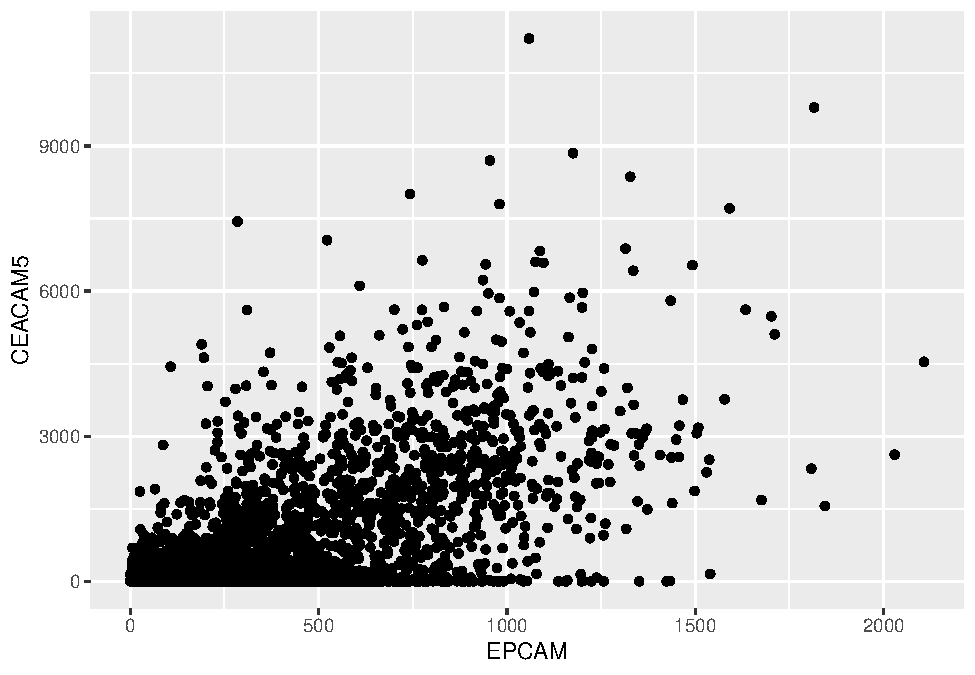
\includegraphics{09_Data_visualization_with_ggplot2_files/figure-latex/unnamed-chunk-6-1.pdf}

In the code above:

\begin{itemize}
\item
  We use ggplot() to initialize a new ggplot2 plot.
\item
  Inside aes(), we specify the aesthetic mappings, where x represents the \texttt{EPCAM} gene expression and y represents the \texttt{CEACAM5} gene expression.
\item
  We add `\texttt{geom\_point()} to plot the data points on the graph.
\end{itemize}

\hypertarget{interpretation}{%
\subsubsection{Interpretation}\label{interpretation}}

The scatter plot visually represents the relationship between the \texttt{EPCAM} and \texttt{CEACAM5} gene expression levels. Each point on the plot corresponds to a cancer sample, with its EPCAM expression on the x-axis and CEACAM5 expression on the y-axis. If the points tend to fall on the diagonal line, it suggests a relationship between the two gene expressions.

\hypertarget{calculating-correlation}{%
\subsection{Calculating Correlation}\label{calculating-correlation}}

To quantify the relationship between \texttt{EPCAM} and \texttt{CEACAM5} gene expressions, we can calculate the Pearson correlation coefficient. This coefficient measures the strength and direction of the linear relationship between two variables.

\begin{Shaded}
\begin{Highlighting}[]
\CommentTok{\# Calculate the Pearson correlation coefficient}
\NormalTok{correlation }\OtherTok{\textless{}{-}} \FunctionTok{cor}\NormalTok{(tcga\_cancer}\SpecialCharTok{$}\NormalTok{EPCAM, tcga\_cancer}\SpecialCharTok{$}\NormalTok{CEACAM5)}
\NormalTok{correlation}
\end{Highlighting}
\end{Shaded}

\begin{verbatim}
## [1] 0.6324328
\end{verbatim}

The output will be a value between -1 and 1, where:

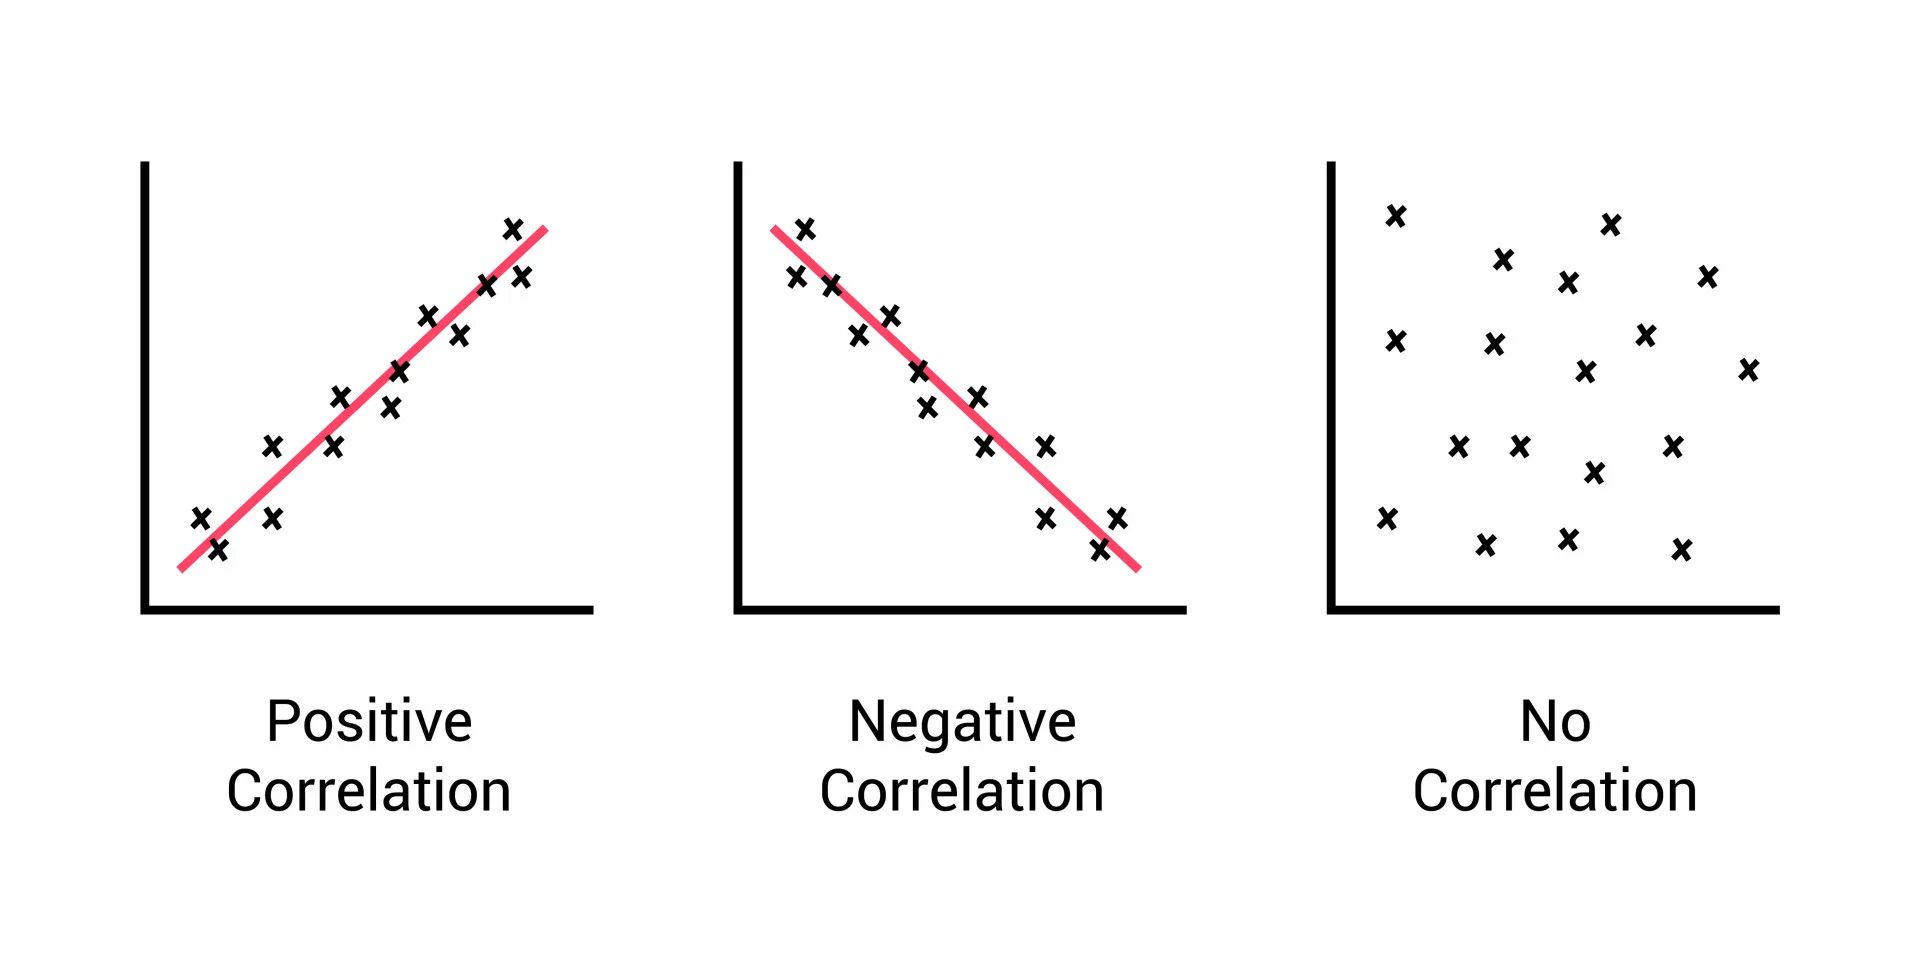
\includegraphics{images/cor.png}

\begin{itemize}
\item
  A positive value (closer to 1) indicates a positive correlation (both variables increase together).
\item
  A negative value (closer to -1) indicates a negative correlation (one variable increases as the other decreases).
\item
  A value close to 0 indicates little to no linear correlation.
\end{itemize}

In our example, the correlation coefficient (Pearson's r) is approximately \texttt{0.6324}, which suggests a moderately positive correlation between \texttt{EPCAM} and \texttt{CEACAM5} gene expressions among cancer samples.

\hypertarget{hypothesis-testing}{%
\subsection{Hypothesis Testing}\label{hypothesis-testing}}

\begin{quote}
Check docs here: \url{https://rdrr.io/r/stats/cor.test.html}
\end{quote}

To determine if this correlation is statistically significant, we can perform a hypothesis test. In our case, we're interested in testing whether the correlation is significantly different from zero.

\begin{Shaded}
\begin{Highlighting}[]
\CommentTok{\# Perform a correlation hypothesis test}
\NormalTok{cor\_test\_result }\OtherTok{\textless{}{-}} \FunctionTok{cor.test}\NormalTok{(tcga\_cancer}\SpecialCharTok{$}\NormalTok{EPCAM, tcga\_cancer}\SpecialCharTok{$}\NormalTok{CEACAM5)}
\NormalTok{cor\_test\_result}
\end{Highlighting}
\end{Shaded}

\begin{verbatim}
## 
##  Pearson's product-moment correlation
## 
## data:  tcga_cancer$EPCAM and tcga_cancer$CEACAM5
## t = 81.722, df = 10019, p-value < 2.2e-16
## alternative hypothesis: true correlation is not equal to 0
## 95 percent confidence interval:
##  0.6205372 0.6440374
## sample estimates:
##       cor 
## 0.6324328
\end{verbatim}

The output will provide various statistics, including the t-value, degrees of freedom, and the p-value.

\hypertarget{interpretation-1}{%
\subsubsection{Interpretation}\label{interpretation-1}}

In the results, you'll see:

\begin{itemize}
\item
  The t-value, which measures the number of standard errors the correlation coefficient is away from zero.
\item
  The degrees of freedom (df), which are related to the sample size.
\item
  The p-value, which tells us whether the correlation is statistically significant.
\end{itemize}

In our case, the p-value is very close to zero (\texttt{p-value\ \textless{}\ 2.2e-16}), indicating strong evidence against the null hypothesis (the true correlation is zero). Therefore, we can conclude that the correlation between EPCAM and CEACAM5 gene expressions is statistically significant. You need to keep in mind that in genomics data analysis, typically you have thousands of samples and you will inherently get tiny p values. In our case, focus on the effect size (in this case, the coefficient value which is 0.63).

\hypertarget{adding-a-regression-line}{%
\subsection{Adding a Regression Line}\label{adding-a-regression-line}}

\begin{quote}
Check docs on geom\_smooth here: \url{https://ggplot2.tidyverse.org/reference/geom_smooth.html}
\end{quote}

To further explore the relationship between the two gene expressions, we can add a linear regression line to our scatter plot using \texttt{geom\_smooth()}.

\begin{Shaded}
\begin{Highlighting}[]
\CommentTok{\# Create a scatter plot with a regression line}
\FunctionTok{ggplot}\NormalTok{(tcga\_cancer, }\FunctionTok{aes}\NormalTok{(}\AttributeTok{x =}\NormalTok{ EPCAM, }\AttributeTok{y =}\NormalTok{ CEACAM5)) }\SpecialCharTok{+}
  \FunctionTok{geom\_point}\NormalTok{() }\SpecialCharTok{+}
  \FunctionTok{geom\_smooth}\NormalTok{(}\AttributeTok{method =} \StringTok{"lm"}\NormalTok{)}
\end{Highlighting}
\end{Shaded}

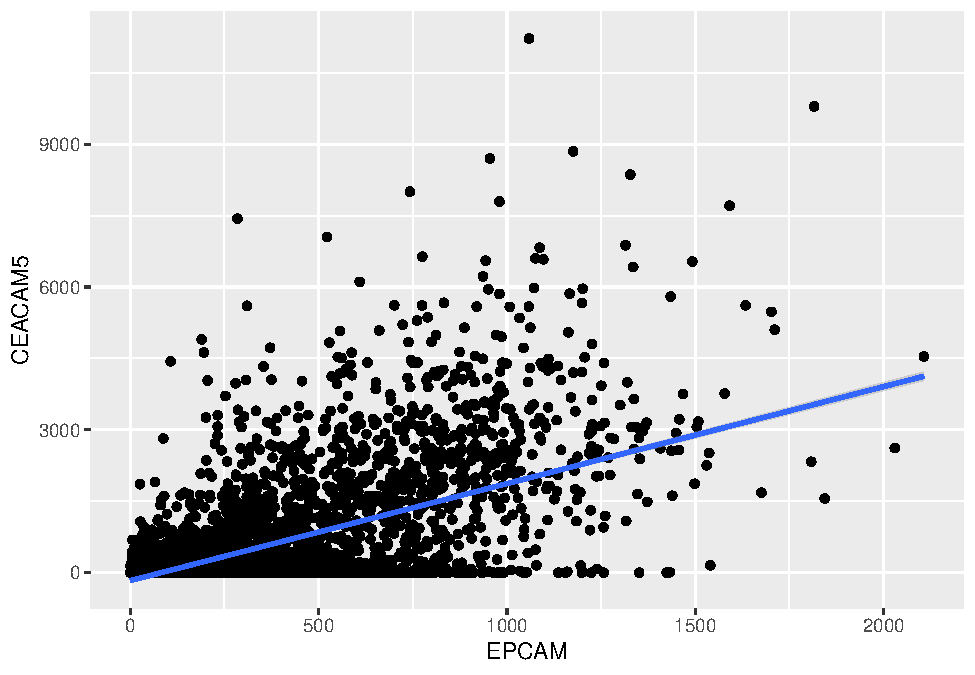
\includegraphics{09_Data_visualization_with_ggplot2_files/figure-latex/unnamed-chunk-9-1.pdf}

The \texttt{geom\_smooth()} function with \texttt{method\ =\ "lm"} fits a linear regression line to the data points, helping us visualize the trend more clearly.

The regression line provides a visual representation of how one gene's expression (EPCAM) changes concerning the other (CEACAM5). If the line slopes upward, it suggests a positive correlation, while a downward slope indicates a negative correlation.

\hypertarget{conclusion-22}{%
\subsection{Conclusion}\label{conclusion-22}}

In this lesson, we've covered the basics of creating scatter plots, calculating correlation coefficients, and performing hypothesis tests using R. These skills are essential for exploring relationships between variables in your data, whether you're analyzing gene expressions, financial data, or any other dataset. Remember that correlation does not imply causation, so it's essential to interpret your findings carefully and consider the context of your analysis.

\hypertarget{understanding-distributions-with-histograms}{%
\section{Understanding Distributions with Histograms}\label{understanding-distributions-with-histograms}}

In this section, we will explore another powerful data visualization tool: histograms. Histograms are especially useful for understanding the distribution of a single numerical variable. We will use R and the ggplot2 package to create histograms and customize them to gain insights into the distribution of gene expression levels.

For this course we're using the data we generated in previous lesson.

\hypertarget{creating-a-basic-histogram}{%
\subsection{Creating a Basic Histogram}\label{creating-a-basic-histogram}}

Let's start by creating a basic histogram to visualize the distribution of the EPCAM gene expression levels across all cancer samples.

\begin{Shaded}
\begin{Highlighting}[]
\CommentTok{\# Create a basic histogram for EPCAM gene expression}
\FunctionTok{ggplot}\NormalTok{(tcga\_cancer, }\FunctionTok{aes}\NormalTok{(}\AttributeTok{x =}\NormalTok{ EPCAM)) }\SpecialCharTok{+}
  \FunctionTok{geom\_histogram}\NormalTok{()}
\end{Highlighting}
\end{Shaded}

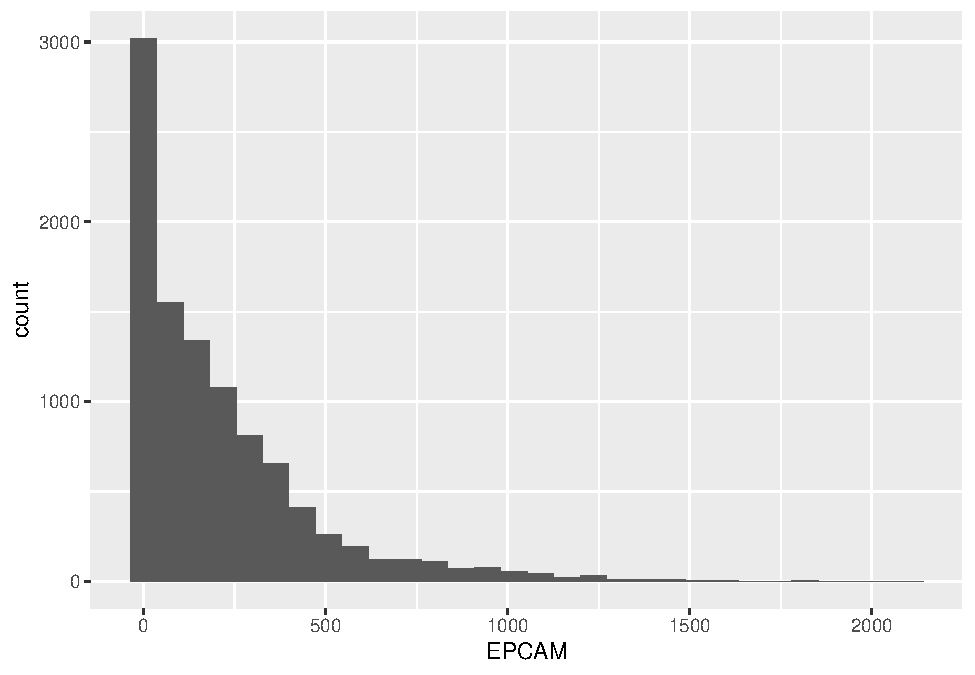
\includegraphics{09_Data_visualization_with_ggplot2_files/figure-latex/unnamed-chunk-10-1.pdf}

In this code:

\begin{itemize}
\item
  We use \texttt{ggplot()} to initialize a new ggplot2 plot.
\item
  Inside \texttt{aes()}, we specify that we want to map the \texttt{EPCAM} gene expression values to the x-axis.
\item
  We add \texttt{geom\_histogram()} to create the histogram.
\end{itemize}

The resulting plot will display the EPCAM gene expression levels on the x-axis and the count of samples falling into each ``bin'' on the y-axis. A bin is a range of values, and the height of each bar represents how many samples have expression levels within that range.

\hypertarget{customizing-histogram-bins}{%
\subsection{Customizing Histogram Bins}\label{customizing-histogram-bins}}

You can customize the granularity of your histogram by changing the number of bins or specifying the bin size. This allows you to get a more detailed or broader view of the data distribution.

\hypertarget{changing-the-number-of-bins}{%
\subsubsection{Changing the Number of Bins}\label{changing-the-number-of-bins}}

To change the number of bins, you can use the bins parameter within geom\_histogram(). Increasing the number of bins provides more detail.

\begin{Shaded}
\begin{Highlighting}[]
\CommentTok{\# Create a histogram with 50 bins}
\FunctionTok{ggplot}\NormalTok{(tcga\_cancer, }\FunctionTok{aes}\NormalTok{(}\AttributeTok{x =}\NormalTok{ EPCAM)) }\SpecialCharTok{+}
  \FunctionTok{geom\_histogram}\NormalTok{(}\AttributeTok{bins =} \DecValTok{50}\NormalTok{)}
\end{Highlighting}
\end{Shaded}

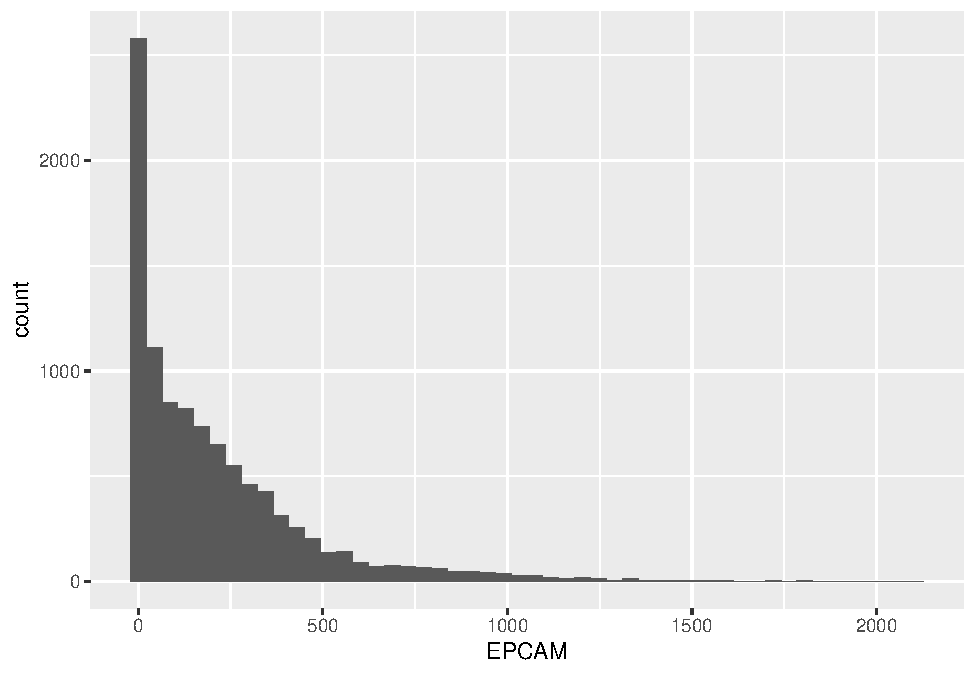
\includegraphics{09_Data_visualization_with_ggplot2_files/figure-latex/unnamed-chunk-11-1.pdf}

\hypertarget{customizing-bin-borders}{%
\subsubsection{Customizing Bin Borders}\label{customizing-bin-borders}}

By default, the borders of the bins in the histogram are not very visible. You can change the border color to white to make them more distinct.

\begin{Shaded}
\begin{Highlighting}[]
\CommentTok{\# Create a histogram with white bin borders}
\FunctionTok{ggplot}\NormalTok{(tcga\_cancer, }\FunctionTok{aes}\NormalTok{(}\AttributeTok{x =}\NormalTok{ EPCAM)) }\SpecialCharTok{+}
  \FunctionTok{geom\_histogram}\NormalTok{(}\AttributeTok{bins =} \DecValTok{50}\NormalTok{, }\AttributeTok{color =} \StringTok{"white"}\NormalTok{)}
\end{Highlighting}
\end{Shaded}

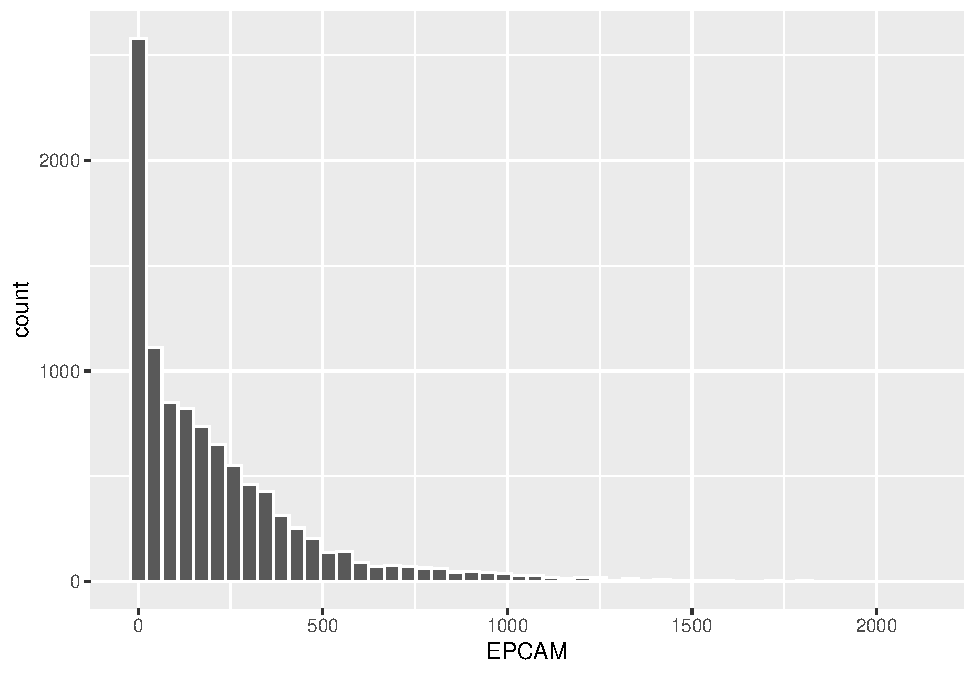
\includegraphics{09_Data_visualization_with_ggplot2_files/figure-latex/unnamed-chunk-12-1.pdf}

Changing the bin border color to white makes it easier to distinguish between adjacent bins.

\hypertarget{conclusion-23}{%
\subsection{Conclusion}\label{conclusion-23}}

Histograms are valuable tools for visualizing the distribution of a single numerical variable, helping you understand the underlying data structure. By customizing the number of bins, bin sizes, and bin borders, you can tailor your histograms to reveal the level of detail you need. Whether you are analyzing gene expression data or any other quantitative data, histograms are an essential part of your data exploration toolkit.

\hypertarget{visualizing-data-distribution-with-boxplots-and-violin-plots}{%
\section{Visualizing Data Distribution with Boxplots and Violin Plots}\label{visualizing-data-distribution-with-boxplots-and-violin-plots}}

In this lesson, we will explore how to visualize the distribution of gene expression data across different cancer types using boxplots and violin plots in R. These graphical tools are invaluable for gaining insights into the spread and central tendency of data within different categories.

We will continue to work with the TCGA gene expression dataset, specifically focusing on cancer samples (tcga\_cancer). This dataset contains various gene expression measurements across different cancer types.

\hypertarget{creating-a-basic-boxplot}{%
\subsection{Creating a Basic Boxplot}\label{creating-a-basic-boxplot}}

Let's start by creating a basic boxplot to visualize the distribution of the EPCAM gene expression across different cancer types.

\begin{Shaded}
\begin{Highlighting}[]
\FunctionTok{library}\NormalTok{(ggplot2)}

\FunctionTok{ggplot}\NormalTok{(tcga\_cancer, }\FunctionTok{aes}\NormalTok{(}\AttributeTok{x =}\NormalTok{ study, }\AttributeTok{y =}\NormalTok{ EPCAM)) }\SpecialCharTok{+}
  \FunctionTok{geom\_boxplot}\NormalTok{()}
\end{Highlighting}
\end{Shaded}

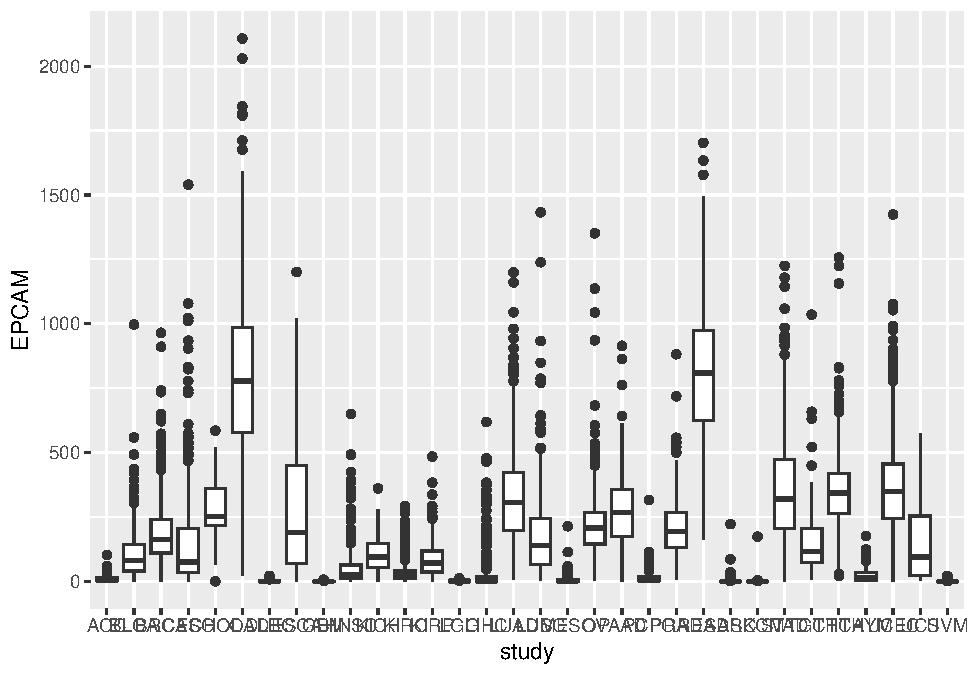
\includegraphics{09_Data_visualization_with_ggplot2_files/figure-latex/unnamed-chunk-13-1.pdf}

In this code:

\begin{itemize}
\item
  We use \texttt{ggplot()} to initialize the plot.
\item
  We map the x-axis to study (representing cancer types) and the y-axis to EPCAM gene expression.
\item
  We add \texttt{geom\_boxplot()} to create the boxplots.
\end{itemize}

\hypertarget{rotating-x-axis-labels}{%
\subsection{Rotating X-axis Labels}\label{rotating-x-axis-labels}}

You may notice that the x-axis labels (cancer types) overlap. To make the plot more readable, we can rotate the x-axis labels by 90 degrees and remove the x-axis label using the \texttt{theme} function.

\begin{Shaded}
\begin{Highlighting}[]
\FunctionTok{ggplot}\NormalTok{(tcga\_cancer, }\FunctionTok{aes}\NormalTok{(}\AttributeTok{x =}\NormalTok{ study, }\AttributeTok{y =}\NormalTok{ EPCAM)) }\SpecialCharTok{+}
  \FunctionTok{geom\_boxplot}\NormalTok{() }\SpecialCharTok{+}
  \FunctionTok{theme}\NormalTok{(}\AttributeTok{axis.text.x =} \FunctionTok{element\_text}\NormalTok{(}\AttributeTok{angle =} \DecValTok{90}\NormalTok{, }\AttributeTok{vjust =} \FloatTok{0.5}\NormalTok{, }\AttributeTok{hjust =} \DecValTok{1}\NormalTok{),}
        \AttributeTok{axis.title.x =} \FunctionTok{element\_blank}\NormalTok{())}
\end{Highlighting}
\end{Shaded}

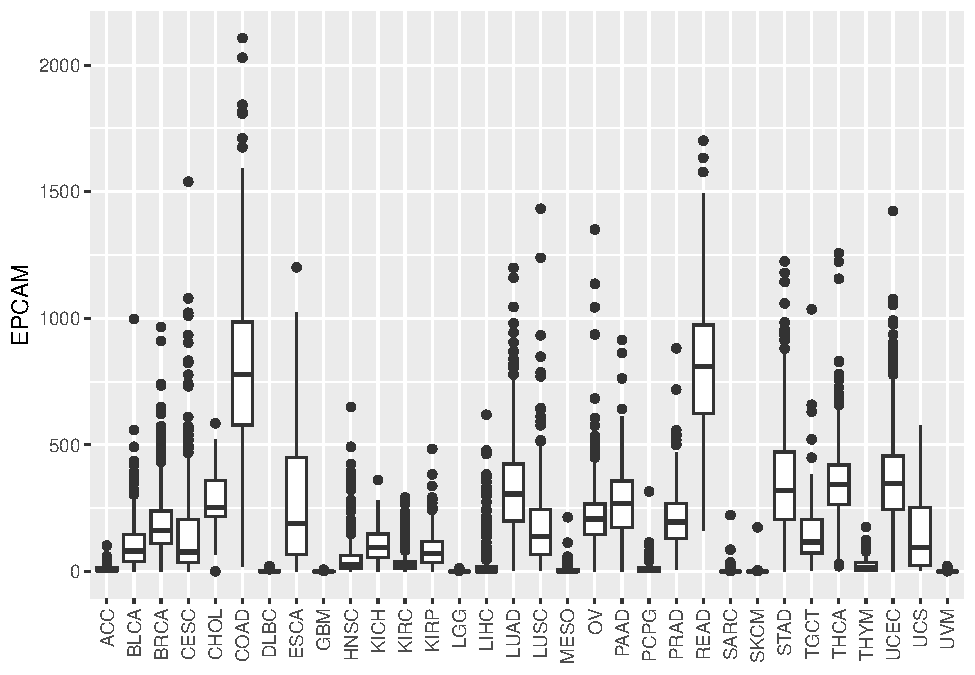
\includegraphics{09_Data_visualization_with_ggplot2_files/figure-latex/test-1.pdf}
Now, the x-axis labels are more legible.

\hypertarget{adding-color-to-boxplots}{%
\subsection{Adding Color to Boxplots}\label{adding-color-to-boxplots}}

To distinguish between cancer types more effectively, let's add color to the boxplots by mapping the color aesthetic to the study.

\begin{Shaded}
\begin{Highlighting}[]
\FunctionTok{ggplot}\NormalTok{(tcga\_cancer, }\FunctionTok{aes}\NormalTok{(}\AttributeTok{x =}\NormalTok{ study, }\AttributeTok{y =}\NormalTok{ EPCAM)) }\SpecialCharTok{+}
  \FunctionTok{geom\_boxplot}\NormalTok{(}\FunctionTok{aes}\NormalTok{(}\AttributeTok{color =}\NormalTok{ study)) }\SpecialCharTok{+}
  \FunctionTok{theme}\NormalTok{(}\AttributeTok{axis.text.x =} \FunctionTok{element\_text}\NormalTok{(}\AttributeTok{angle =} \DecValTok{90}\NormalTok{, }\AttributeTok{vjust =} \FloatTok{0.5}\NormalTok{, }\AttributeTok{hjust =} \DecValTok{1}\NormalTok{),}
        \AttributeTok{axis.title.x =} \FunctionTok{element\_blank}\NormalTok{())}
\end{Highlighting}
\end{Shaded}

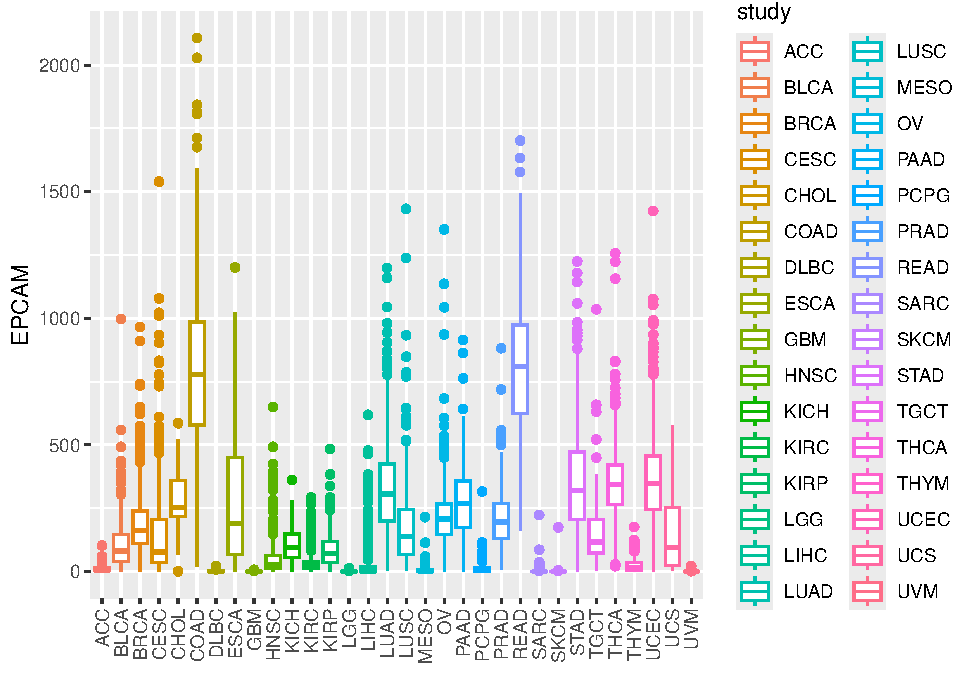
\includegraphics{09_Data_visualization_with_ggplot2_files/figure-latex/unnamed-chunk-14-1.pdf}

Alternatively, you can use \texttt{fill} to color the boxes instead of the outlines:

\begin{Shaded}
\begin{Highlighting}[]
\FunctionTok{ggplot}\NormalTok{(tcga\_cancer, }\FunctionTok{aes}\NormalTok{(}\AttributeTok{x =}\NormalTok{ study, }\AttributeTok{y =}\NormalTok{ EPCAM)) }\SpecialCharTok{+}
  \FunctionTok{geom\_boxplot}\NormalTok{(}\FunctionTok{aes}\NormalTok{(}\AttributeTok{fill =}\NormalTok{ study)) }\SpecialCharTok{+}
  \FunctionTok{theme}\NormalTok{(}\AttributeTok{axis.text.x =} \FunctionTok{element\_text}\NormalTok{(}\AttributeTok{angle =} \DecValTok{90}\NormalTok{, }\AttributeTok{vjust =} \FloatTok{0.5}\NormalTok{, }\AttributeTok{hjust =} \DecValTok{1}\NormalTok{),}
        \AttributeTok{axis.title.x =} \FunctionTok{element\_blank}\NormalTok{())}
\end{Highlighting}
\end{Shaded}

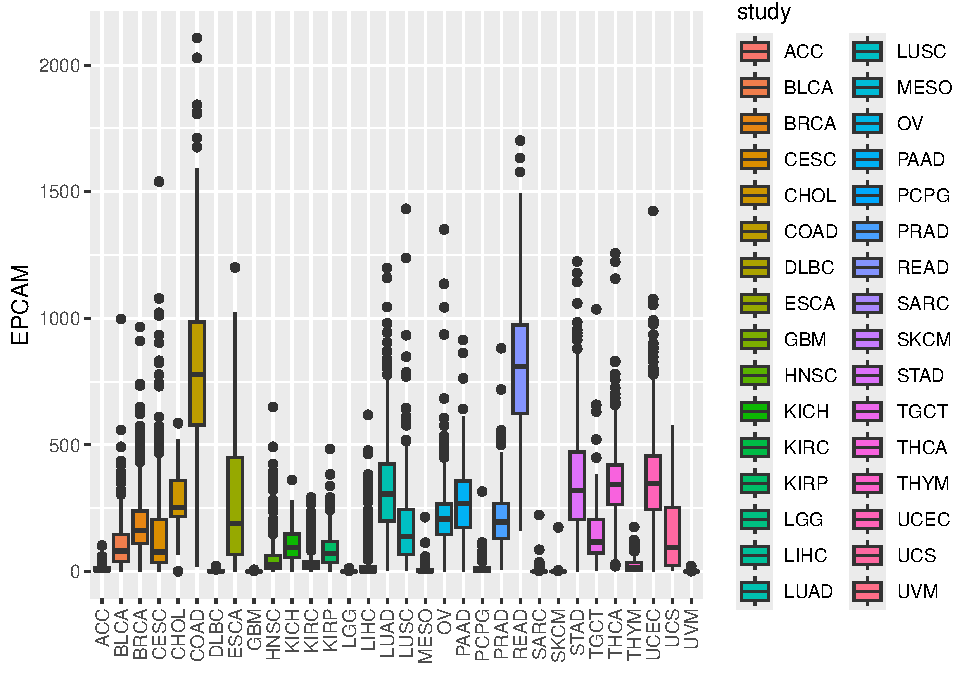
\includegraphics{09_Data_visualization_with_ggplot2_files/figure-latex/unnamed-chunk-15-1.pdf}

By default, ggplot2 uses a default color palette, but you can specify colors manually if needed.

\hypertarget{customizing-color-palettes}{%
\subsection{Customizing Color Palettes}\label{customizing-color-palettes}}

In case you want to define your color palette for the cancer types, you can use the Polychrome package.

\begin{Shaded}
\begin{Highlighting}[]
\CommentTok{\# there are total 32 cancer types}
\FunctionTok{length}\NormalTok{(}\FunctionTok{unique}\NormalTok{(tcga\_cancer}\SpecialCharTok{$}\NormalTok{study))}
\end{Highlighting}
\end{Shaded}

\begin{verbatim}
## [1] 32
\end{verbatim}

Here's how to create a custom color palette for 32 cancer types:

\begin{Shaded}
\begin{Highlighting}[]
\CommentTok{\# install.packages("Polychrome")}
\FunctionTok{library}\NormalTok{(Polychrome)}

\CommentTok{\# There are a total of 32 cancer types}
\FunctionTok{length}\NormalTok{(}\FunctionTok{unique}\NormalTok{(tcga\_cancer}\SpecialCharTok{$}\NormalTok{study))}
\end{Highlighting}
\end{Shaded}

\begin{verbatim}
## [1] 32
\end{verbatim}

\begin{Shaded}
\begin{Highlighting}[]
\CommentTok{\# Create a custom color palette with Polychrome}
\NormalTok{P32 }\OtherTok{\textless{}{-}} \FunctionTok{createPalette}\NormalTok{(}\DecValTok{32}\NormalTok{, }\FunctionTok{c}\NormalTok{(}\StringTok{"\#FF0000"}\NormalTok{, }\StringTok{"\#00FF00"}\NormalTok{, }\StringTok{"\#0000FF"}\NormalTok{), }\AttributeTok{range =} \FunctionTok{c}\NormalTok{(}\DecValTok{30}\NormalTok{, }\DecValTok{80}\NormalTok{))}

\NormalTok{P32}
\end{Highlighting}
\end{Shaded}

\begin{verbatim}
##       NC1       NC2       NC3       NC4       NC5       NC6       NC7       NC8 
## "#FB1C16" "#0DE100" "#2216FA" "#EBB7BF" "#FC00E3" "#00D0FD" "#FF9516" "#0D7745" 
##       NC9      NC10      NC11      NC12      NC13      NC14      NC15      NC16 
## "#D0CB1C" "#D53576" "#623589" "#CC66FD" "#803D0D" "#DD70C2" "#708DA0" "#869BFE" 
##      NC17      NC18      NC19      NC20      NC21      NC22      NC23      NC24 
## "#1CDDCA" "#9B8F53" "#92D86D" "#DAB6FA" "#F45D4B" "#753D5A" "#FD928B" "#F0B660" 
##      NC25      NC26      NC27      NC28      NC29      NC30      NC31      NC32 
## "#ACCEB2" "#FF1C71" "#F100AD" "#006EA7" "#22DF97" "#691CBF" "#9900A0" "#911C51"
\end{verbatim}

You see the \href{https://en.wikipedia.org/wiki/Web_colors}{hex code} for the colors.

Now, we have a custom color palette P32 with 32 unique colors. You can visualize the colors using \texttt{swatch(P32)} in the polychrom package.

\begin{Shaded}
\begin{Highlighting}[]
\FunctionTok{swatch}\NormalTok{(P32)}
\end{Highlighting}
\end{Shaded}

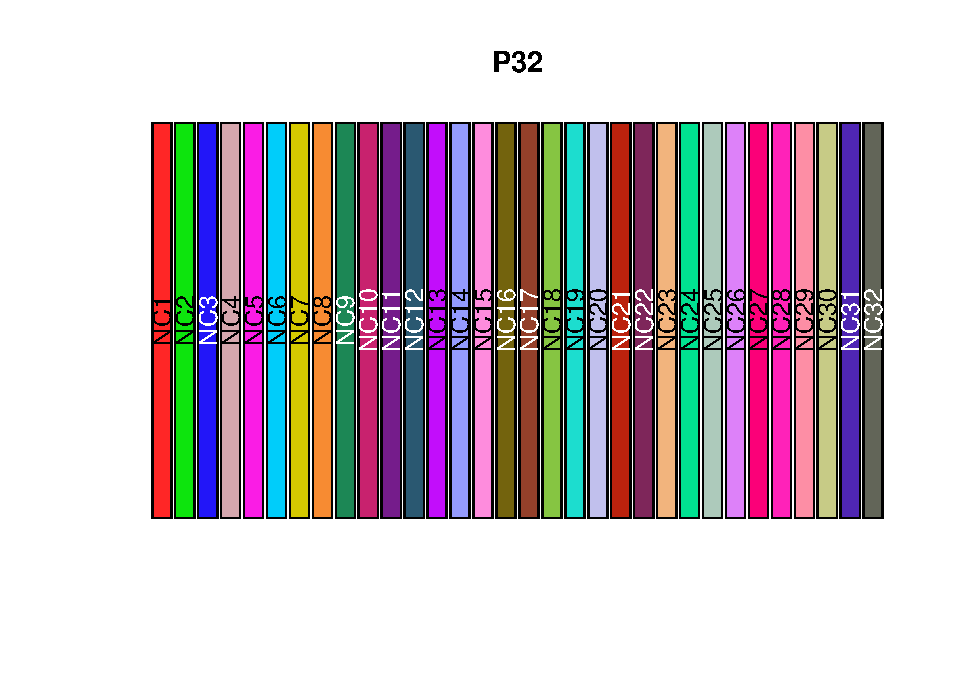
\includegraphics{09_Data_visualization_with_ggplot2_files/figure-latex/unnamed-chunk-18-1.pdf}

\hypertarget{applying-custom-color-palette}{%
\subsection{Applying Custom Color Palette}\label{applying-custom-color-palette}}

To use the custom color palette with your boxplot, use \texttt{scale\_fill\_manual()} or \texttt{scale\_color\_manual()} to map the colors manually to the study variable.

\begin{Shaded}
\begin{Highlighting}[]
\FunctionTok{ggplot}\NormalTok{(tcga\_cancer, }\FunctionTok{aes}\NormalTok{(}\AttributeTok{x =}\NormalTok{ study, }\AttributeTok{y =}\NormalTok{ EPCAM)) }\SpecialCharTok{+}
  \FunctionTok{geom\_boxplot}\NormalTok{(}\FunctionTok{aes}\NormalTok{(}\AttributeTok{fill =}\NormalTok{ study)) }\SpecialCharTok{+}
  \FunctionTok{scale\_fill\_manual}\NormalTok{(}\AttributeTok{values =} \FunctionTok{unname}\NormalTok{(P32)) }\SpecialCharTok{+}
  \FunctionTok{theme}\NormalTok{(}\AttributeTok{axis.text.x =} \FunctionTok{element\_text}\NormalTok{(}\AttributeTok{angle =} \DecValTok{90}\NormalTok{, }\AttributeTok{vjust =} \FloatTok{0.5}\NormalTok{, }\AttributeTok{hjust =} \DecValTok{1}\NormalTok{),}
        \AttributeTok{axis.title.x =} \FunctionTok{element\_blank}\NormalTok{())}
\end{Highlighting}
\end{Shaded}

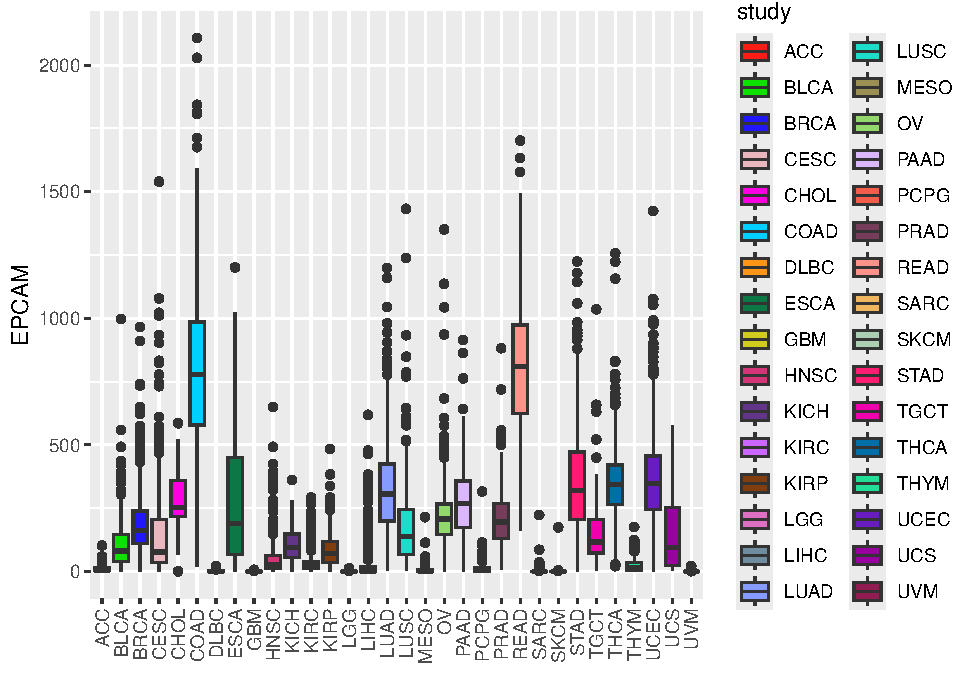
\includegraphics{09_Data_visualization_with_ggplot2_files/figure-latex/unnamed-chunk-19-1.pdf}
Note, you need to remove the names of the named color vector using \texttt{unname}.

Now, the boxplot colors are based on your custom palette, making it more visually appealing and distinct.

\hypertarget{reordering-boxplots}{%
\subsection{Reordering Boxplots}\label{reordering-boxplots}}

To reorder the boxes according to the median level of EPCAM expression, you can use the \texttt{forcats::fct\_reorder()} function within your \texttt{aes()} mapping.

\begin{Shaded}
\begin{Highlighting}[]
\FunctionTok{ggplot}\NormalTok{(tcga\_cancer, }\FunctionTok{aes}\NormalTok{(}\AttributeTok{x =}\NormalTok{ study }\SpecialCharTok{\%\textgreater{}\%}
\NormalTok{                          forcats}\SpecialCharTok{::}\FunctionTok{fct\_reorder}\NormalTok{(EPCAM, median), }
                        \AttributeTok{y =}\NormalTok{ EPCAM)) }\SpecialCharTok{+}
  \FunctionTok{geom\_boxplot}\NormalTok{(}\FunctionTok{aes}\NormalTok{(}\AttributeTok{fill =}\NormalTok{ study)) }\SpecialCharTok{+}
  \FunctionTok{scale\_fill\_manual}\NormalTok{(}\AttributeTok{values =} \FunctionTok{unname}\NormalTok{(P32)) }\SpecialCharTok{+}
  \FunctionTok{theme}\NormalTok{(}\AttributeTok{axis.text.x =} \FunctionTok{element\_text}\NormalTok{(}\AttributeTok{angle =} \DecValTok{90}\NormalTok{, }\AttributeTok{vjust =} \FloatTok{0.5}\NormalTok{, }\AttributeTok{hjust =} \DecValTok{1}\NormalTok{),}
        \AttributeTok{axis.title.x =} \FunctionTok{element\_blank}\NormalTok{())}
\end{Highlighting}
\end{Shaded}

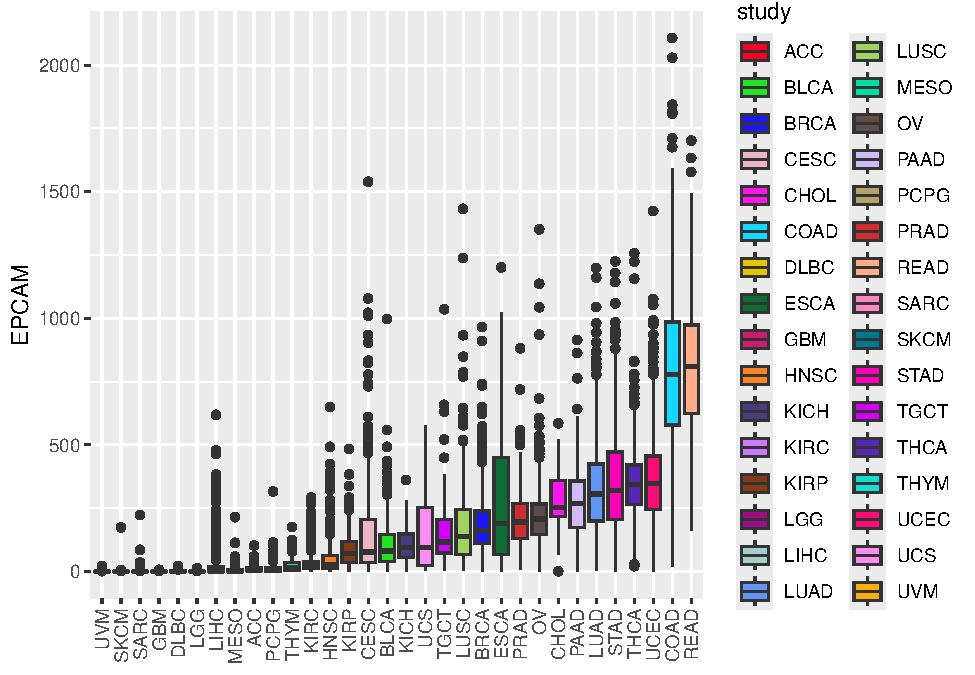
\includegraphics{09_Data_visualization_with_ggplot2_files/figure-latex/unnamed-chunk-20-1.pdf}

The \texttt{forcats::fct\_reorder()} function takes two arguments:

\begin{itemize}
\item
  The first argument (study) is the factor variable whose levels we want to reorder.
\item
  The second argument (EPCAM) is the numeric variable based on which the reordering will be done (in this case, the median expression levels of EPCAM).
\end{itemize}

As a result of this reordering, the levels of the study factor will be rearranged from low to high median EPCAM expression levels. Now, the boxes are arranged from low to high EPCAM expression levels, providing a clearer view of the data distribution.

\hypertarget{using-violin-plots}{%
\subsection{Using Violin Plots}\label{using-violin-plots}}

Violin plots combine a boxplot with a kernel density plot, allowing you to visualize both the summary statistics and the entire data distribution.

\begin{Shaded}
\begin{Highlighting}[]
\FunctionTok{ggplot}\NormalTok{(tcga\_cancer, }\FunctionTok{aes}\NormalTok{(}\AttributeTok{x =}\NormalTok{ study }\SpecialCharTok{\%\textgreater{}\%}
\NormalTok{                          forcats}\SpecialCharTok{::}\FunctionTok{fct\_reorder}\NormalTok{(EPCAM, median), }
                        \AttributeTok{y =}\NormalTok{ EPCAM)) }\SpecialCharTok{+}
  \FunctionTok{geom\_violin}\NormalTok{(}\FunctionTok{aes}\NormalTok{(}\AttributeTok{fill =}\NormalTok{ study), }\AttributeTok{scale =} \StringTok{"width"}\NormalTok{) }\SpecialCharTok{+}
  \FunctionTok{scale\_fill\_manual}\NormalTok{(}\AttributeTok{values =} \FunctionTok{unname}\NormalTok{(P32)) }\SpecialCharTok{+}
  \FunctionTok{theme}\NormalTok{(}\AttributeTok{axis.text.x =} \FunctionTok{element\_text}\NormalTok{(}\AttributeTok{angle =} \DecValTok{90}\NormalTok{, }\AttributeTok{vjust =} \FloatTok{0.5}\NormalTok{, }\AttributeTok{hjust =} \DecValTok{1}\NormalTok{),}
        \AttributeTok{axis.title.x =} \FunctionTok{element\_blank}\NormalTok{())}
\end{Highlighting}
\end{Shaded}

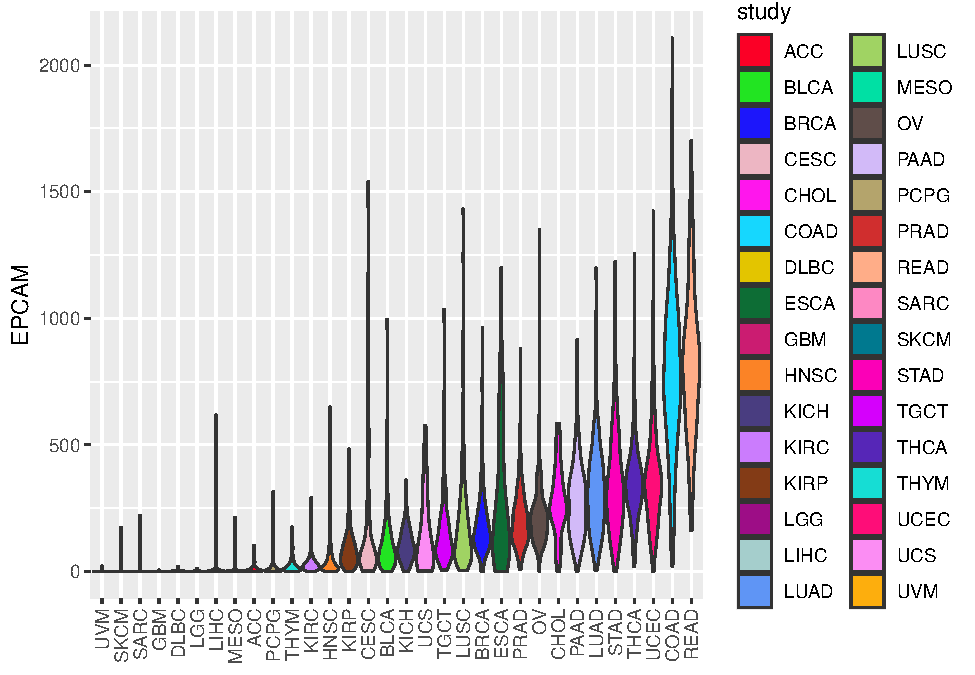
\includegraphics{09_Data_visualization_with_ggplot2_files/figure-latex/unnamed-chunk-21-1.pdf}

In this code, we replaced \texttt{geom\_boxplot} with \texttt{geom\_violin} to create a violin plot. The width of the violin plots is scaled for better visibility.

\hypertarget{conclusion-24}{%
\subsection{Conclusion}\label{conclusion-24}}

In this lesson, we've explored how to visualize data distribution using boxplots and violin plots in R. These techniques are essential for understanding the spread and central tendencies of data within different categories or groups. By customizing colors, reordering boxes, and using violin plots, you can effectively communicate insights from your data to others.

\hypertarget{creating-bar-plots-to-visualize-median-epcam-levels-by-cancer-type}{%
\section{Creating Bar Plots to Visualize Median EPCAM Levels by Cancer Type}\label{creating-bar-plots-to-visualize-median-epcam-levels-by-cancer-type}}

In this section, we will learn how to create informative bar plots using R. Specifically, we'll use bar plots to display the median levels of the EPCAM gene expression for different types of cancer. This visualization will help us understand how EPCAM expression varies across various cancer studies. We will also explore techniques to reorder and customize our bar plots for better data interpretation.

\hypertarget{calculating-median-epcam-levels-by-cancer-type}{%
\subsection{Calculating Median EPCAM Levels by Cancer Type}\label{calculating-median-epcam-levels-by-cancer-type}}

The median EPCAM expression levels represent the middle value of EPCAM gene expression measurements for different types of cancer studies, providing a central measure to understand how this gene behaves in each type of cancer.

To begin, we'll calculate the median EPCAM expression levels for each cancer study type. We will create a summary table that includes the cancer study names and their corresponding median EPCAM values.

\begin{Shaded}
\begin{Highlighting}[]
\CommentTok{\# Calculate median EPCAM levels by cancer type}
\NormalTok{EPCAM\_median }\OtherTok{\textless{}{-}}\NormalTok{ tcga\_cancer }\SpecialCharTok{\%\textgreater{}\%}
  \FunctionTok{group\_by}\NormalTok{(study) }\SpecialCharTok{\%\textgreater{}\%}
  \FunctionTok{summarize}\NormalTok{(}\AttributeTok{median\_EPCAM =} \FunctionTok{median}\NormalTok{(EPCAM))}

\CommentTok{\# Display the summary table}
\NormalTok{EPCAM\_median}
\end{Highlighting}
\end{Shaded}

\begin{verbatim}
## # A tibble: 32 x 2
##    study median_EPCAM
##    <chr>        <dbl>
##  1 ACC          4.83 
##  2 BLCA        81.1  
##  3 BRCA       162.   
##  4 CESC        75.9  
##  5 CHOL       251.   
##  6 COAD       778.   
##  7 DLBC         0.578
##  8 ESCA       189.   
##  9 GBM          0.307
## 10 HNSC        24.7  
## # i 22 more rows
\end{verbatim}

This table now shows the median EPCAM expression levels for each cancer study type, making it easier to compare across different types of cancer.

\hypertarget{creating-a-basic-bar-plot}{%
\subsection{Creating a Basic Bar Plot}\label{creating-a-basic-bar-plot}}

Now, let's create a simple bar plot to visualize these median EPCAM levels. We will use \texttt{geom\_bar()} to create bars representing the median values.

\begin{Shaded}
\begin{Highlighting}[]
\FunctionTok{library}\NormalTok{(ggplot2)}

\CommentTok{\# Create a basic bar plot}
\FunctionTok{ggplot}\NormalTok{(EPCAM\_median, }\FunctionTok{aes}\NormalTok{(}\AttributeTok{x =}\NormalTok{ study, }\AttributeTok{y =}\NormalTok{ median\_EPCAM)) }\SpecialCharTok{+}
  \FunctionTok{geom\_bar}\NormalTok{(}\AttributeTok{stat =} \StringTok{"identity"}\NormalTok{) }\SpecialCharTok{+}
  \FunctionTok{theme}\NormalTok{(}\AttributeTok{axis.text.x =} \FunctionTok{element\_text}\NormalTok{(}\AttributeTok{angle =} \DecValTok{90}\NormalTok{, }\AttributeTok{vjust =} \FloatTok{0.5}\NormalTok{, }\AttributeTok{hjust =} \DecValTok{1}\NormalTok{),}
        \AttributeTok{axis.title.x =} \FunctionTok{element\_blank}\NormalTok{())}
\end{Highlighting}
\end{Shaded}

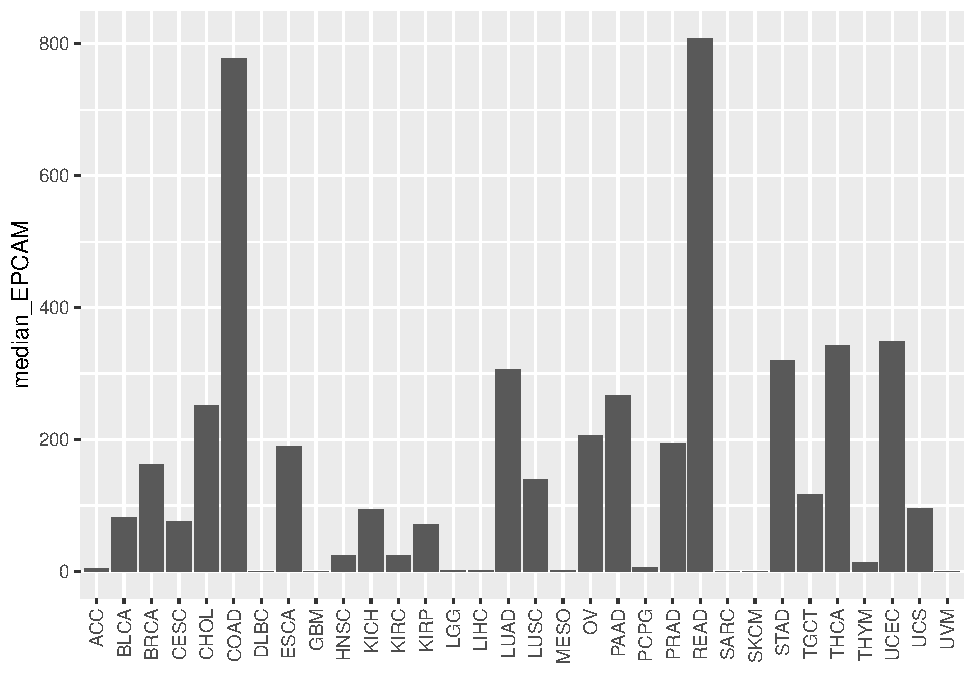
\includegraphics{09_Data_visualization_with_ggplot2_files/figure-latex/unnamed-chunk-23-1.pdf}

In this code:

\begin{itemize}
\item
  We use \texttt{ggplot()} to initialize the plot.
\item
  \texttt{aes()} specifies the aesthetic mappings, where \texttt{x} represents the cancer study names, and \texttt{y} represents the median EPCAM values.
\item
  \texttt{geom\_bar(stat\ =\ "identity")} creates bars where the height of each bar corresponds to the median EPCAM value.
\item
  \texttt{theme()} is used to customize the appearance of the plot, including rotating the x-axis labels for better readability.
\end{itemize}

The basic bar plot displays the median EPCAM levels for each cancer study type, but the bars are not ordered based on the values. We can improve the plot by reordering the bars according to the median EPCAM levels.

\hypertarget{reordering-the-bars}{%
\subsection{Reordering the Bars}\label{reordering-the-bars}}

To make our bar plot more informative, let's reorder the bars based on the median EPCAM values. We can use the \texttt{forcats::fct\_reorder()} function to achieve this.

\begin{Shaded}
\begin{Highlighting}[]
\CommentTok{\# Reorder the bars based on median EPCAM values}
\FunctionTok{ggplot}\NormalTok{(EPCAM\_median, }\FunctionTok{aes}\NormalTok{(}\AttributeTok{x =}\NormalTok{ study }\SpecialCharTok{\%\textgreater{}\%}
\NormalTok{                           forcats}\SpecialCharTok{::}\FunctionTok{fct\_reorder}\NormalTok{(median\_EPCAM), }
                         \AttributeTok{y =}\NormalTok{ median\_EPCAM)) }\SpecialCharTok{+}
  \FunctionTok{geom\_bar}\NormalTok{(}\AttributeTok{stat =} \StringTok{"identity"}\NormalTok{) }\SpecialCharTok{+}
  \FunctionTok{theme}\NormalTok{(}\AttributeTok{axis.text.x =} \FunctionTok{element\_text}\NormalTok{(}\AttributeTok{angle =} \DecValTok{90}\NormalTok{, }\AttributeTok{vjust =} \FloatTok{0.5}\NormalTok{, }\AttributeTok{hjust =} \DecValTok{1}\NormalTok{),}
        \AttributeTok{axis.title.x =} \FunctionTok{element\_blank}\NormalTok{())}
\end{Highlighting}
\end{Shaded}

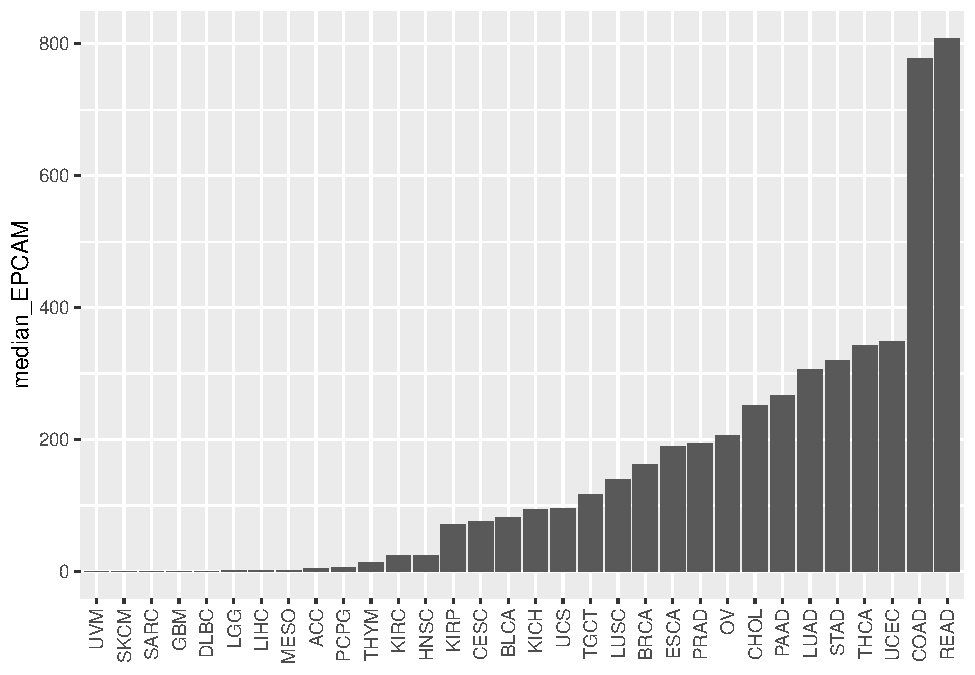
\includegraphics{09_Data_visualization_with_ggplot2_files/figure-latex/unnamed-chunk-24-1.pdf}

In this code:

We use \texttt{forcats::fct\_reorder()} within \texttt{aes()} to reorder the study variable based on the \texttt{median\_EPCAM} values.

The \texttt{median\_EPCAM} values determine the order of the bars from lowest to highest.

Now, the bars are reordered based on the median EPCAM levels, allowing for easier comparison between different cancer study types. This visualization provides insights into which studies exhibit higher or lower median EPCAM expression levels.

\hypertarget{reversing-the-order}{%
\subsection{Reversing the Order}\label{reversing-the-order}}

If you want to reverse the order of the bars, you can use the .desc = TRUE argument with \texttt{forcats::fct\_reorder()}.

\begin{Shaded}
\begin{Highlighting}[]
\CommentTok{\# Reverse the order of the bars}
\FunctionTok{ggplot}\NormalTok{(EPCAM\_median, }\FunctionTok{aes}\NormalTok{(}\AttributeTok{x =}\NormalTok{ study }\SpecialCharTok{\%\textgreater{}\%}
\NormalTok{                           forcats}\SpecialCharTok{::}\FunctionTok{fct\_reorder}\NormalTok{(median\_EPCAM, }\AttributeTok{.desc =} \ConstantTok{TRUE}\NormalTok{), }
                         \AttributeTok{y =}\NormalTok{ median\_EPCAM)) }\SpecialCharTok{+}
  \FunctionTok{geom\_bar}\NormalTok{(}\AttributeTok{stat =} \StringTok{"identity"}\NormalTok{) }\SpecialCharTok{+}
  \FunctionTok{theme}\NormalTok{(}\AttributeTok{axis.text.x =} \FunctionTok{element\_text}\NormalTok{(}\AttributeTok{angle =} \DecValTok{90}\NormalTok{, }\AttributeTok{vjust =} \FloatTok{0.5}\NormalTok{, }\AttributeTok{hjust =} \DecValTok{1}\NormalTok{),}
        \AttributeTok{axis.title.x =} \FunctionTok{element\_blank}\NormalTok{())}
\end{Highlighting}
\end{Shaded}

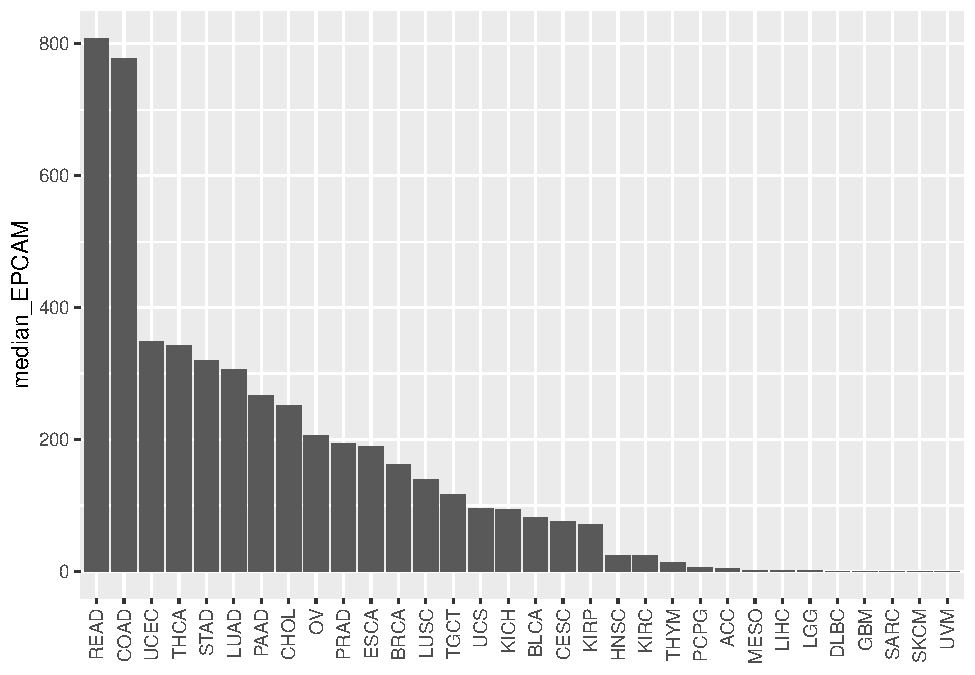
\includegraphics{09_Data_visualization_with_ggplot2_files/figure-latex/unnamed-chunk-25-1.pdf}

By specifying \texttt{.desc\ =\ TRUE}, the bars will be reordered in descending order based on the median EPCAM values.

\hypertarget{note-on-factor-levels}{%
\subsection{Note on factor levels}\label{note-on-factor-levels}}

xxxx

\hypertarget{conclusion-25}{%
\subsection{Conclusion}\label{conclusion-25}}

In this lesson, we have learned how to create bar plots to visualize median EPCAM expression levels by different cancer study types. We explored the process of reordering bars based on values, allowing us to better compare and interpret the data. The order of the bar depends on the factor levels of the study and we used fct\_reorder to accomplish that. Remember that effective data visualization can greatly enhance your ability to communicate insights and make data-driven decisions.

\hypertarget{introduction-to-bioconductor}{%
\chapter{Introduction to BioConductor}\label{introduction-to-bioconductor}}

In the ever-evolving field of bioinformatics and computational biology, researchers and scientists rely on specialized tools and packages to analyze and interpret biological data efficiently. \href{https://bioconductor.org/}{\texttt{Bioconductor}}, a powerful and comprehensive suite of R packages, plays a pivotal role in addressing the unique challenges posed by genomics, transcriptomics, proteomics, and other biological data domains.

This section, ``Introduction to Bioconductor in R,'' will serve as your gateway to this remarkable resource. We will explore the fundamentals of Bioconductor, its significance in the realm of life sciences, and how you can harness its capabilities to unlock valuable insights from complex biological datasets. Whether you are a biologist, bioinformatician, or data scientist, understanding Bioconductor is a crucial step towards advancing your research and data analysis endeavors in the field of biology. Let's embark on this exciting journey into the world of Bioconductor, where data meets discovery.

\hypertarget{introduction-to-biocmanager}{%
\section{Introduction to BiocManager}\label{introduction-to-biocmanager}}

\texttt{BiocManager} is an R package that serves as the primary interface for managing \texttt{Bioconductor} packages, which are extensions of R developed specifically for bioinformatics applications. Bioconductor itself is a project that provides tools for the analysis and comprehension of high-throughput genomic data, including but not limited to next-generation sequencing (NGS), microarrays, and proteomics.

\hypertarget{why-use-biocmanager}{%
\subsection{Why Use BiocManager?}\label{why-use-biocmanager}}

The role of BiocManager is ensuring compatibility among Bioconductor packages and between these packages and your version of R. It simplifies the process of installing Bioconductor packages, managing dependencies, and keeping packages up-to-date with the latest releases, thereby fostering a stable and efficient bioinformatics workflow.

\hypertarget{installing-biocmanager}{%
\subsection{Installing BiocManager}\label{installing-biocmanager}}

To get started with BiocManager, you first need to install it from CRAN (the Comprehensive R Archive Network), which can be done using the following command in R:

\begin{Shaded}
\begin{Highlighting}[]
\FunctionTok{install.packages}\NormalTok{(}\StringTok{"BiocManager"}\NormalTok{)}
\end{Highlighting}
\end{Shaded}

Once installed, you can load \texttt{BiocManager} just like any other R package:

\begin{Shaded}
\begin{Highlighting}[]
\FunctionTok{library}\NormalTok{(BiocManager)}
\end{Highlighting}
\end{Shaded}

\hypertarget{installing-bioconductor-packages}{%
\subsection{Installing Bioconductor Packages}\label{installing-bioconductor-packages}}

With \texttt{BiocManager} loaded, installing Bioconductor packages is straightforward. Suppose you want to install the \texttt{GenomicRanges} package; you can do so with the following command:

\begin{Shaded}
\begin{Highlighting}[]
\NormalTok{BiocManager}\SpecialCharTok{::}\FunctionTok{install}\NormalTok{(}\StringTok{"GenomicRanges"}\NormalTok{)}
\end{Highlighting}
\end{Shaded}

BiocManager automatically resolves and installs any dependencies, ensuring that all required packages are installed for the \texttt{GenomicRanges} package to function correctly.

\hypertarget{updating-bioconductor-packages}{%
\subsection{Updating Bioconductor Packages}\label{updating-bioconductor-packages}}

Keeping your Bioconductor packages up-to-date is crucial for accessing the latest features, improvements, and bug fixes. BiocManager facilitates this through the install function, which also checks for and updates any out-of-date packages:

\begin{Shaded}
\begin{Highlighting}[]
\NormalTok{BiocManager}\SpecialCharTok{::}\FunctionTok{install}\NormalTok{()}
\end{Highlighting}
\end{Shaded}

Running this command without specifying a package name updates all installed Bioconductor packages to their latest versions.

\hypertarget{checking-for-valid-bioconductor-versions}{%
\subsection{Checking for Valid Bioconductor Versions}\label{checking-for-valid-bioconductor-versions}}

Compatibility between your R version and Bioconductor packages is vital for smooth bioinformatics analyses. BiocManager offers a function to validate this compatibility:

\begin{Shaded}
\begin{Highlighting}[]
\NormalTok{BiocManager}\SpecialCharTok{::}\FunctionTok{valid}\NormalTok{()}
\end{Highlighting}
\end{Shaded}

This command checks that all installed Bioconductor packages are compatible with each other and with your current version of R, providing a report of any inconsistencies.

\hypertarget{conclusion-26}{%
\subsection{Conclusion}\label{conclusion-26}}

\texttt{BiocManager} is an indispensable tool for bioinformatics practitioners working with R and \texttt{Bioconductor}. It simplifies package management, ensuring that researchers can focus on their analyses without being bogged down by software compatibility issues. By leveraging \texttt{BiocManager}, you can maintain a cutting-edge bioinformatics toolkit, fully equipped to tackle the challenges of genomic data analysis.

\hypertarget{working-with-genomic-coordinates-and-regions-in-r}{%
\section{Working with Genomic Coordinates and Regions in R}\label{working-with-genomic-coordinates-and-regions-in-r}}

Genomic coordinates are fundamental in the field of genomics. Whether you're dealing with genes, regulatory elements, ChIP-seq peaks, or mutation calling data, they are all represented as genomic coordinates. In R, you can efficiently handle genomic coordinates and regions using the \texttt{GenomicRanges} package and related tools. In this guide, we'll explore how to work with genomic ranges, extract relevant information, and perform common operations.

\begin{quote}
For a complete overview check docs here: \url{https://bioconductor.org/packages/release/bioc/vignettes/GenomicRanges/inst/doc/GenomicRangesIntroduction.html}
\end{quote}

\hypertarget{introduction-to-genomicranges}{%
\subsection{Introduction to GenomicRanges}\label{introduction-to-genomicranges}}

The \texttt{GenomicRanges} package in R provides data structures for storing and manipulating genomic ranges. A genomic range typically includes information about the chromosome (seqname), the start and end positions, and the strand of the sequence.

\begin{enumerate}
\def\labelenumi{\arabic{enumi}.}
\item
  Every gene or regulatory element (promoters, enhancers) in the genome can be represented in chromosome: start-end format.
\item
  You get a peak file from a ChIP-seq experiment. The peak file is usually represented in a at least 3-column bed format: chromosome, start and end.
\item
  You get a mutation calling \href{https://genome.ucsc.edu/goldenPath/help/vcf.html}{VCF} file. You will have the chromosome and position of that single variant.
\end{enumerate}

Let's start by creating a simple genomic range:

\begin{Shaded}
\begin{Highlighting}[]
\FunctionTok{library}\NormalTok{(GenomicRanges)}

\CommentTok{\# Create a GenomicRanges object}
\NormalTok{gr }\OtherTok{\textless{}{-}} \FunctionTok{GRanges}\NormalTok{(}\AttributeTok{seqnames =} \StringTok{"chr1"}\NormalTok{, }
              \AttributeTok{ranges =} \FunctionTok{IRanges}\NormalTok{(}\DecValTok{1}\SpecialCharTok{:}\DecValTok{10}\NormalTok{, }\AttributeTok{width =} \DecValTok{3}\NormalTok{))}

\NormalTok{gr}
\end{Highlighting}
\end{Shaded}

\begin{verbatim}
## GRanges object with 10 ranges and 0 metadata columns:
##        seqnames    ranges strand
##           <Rle> <IRanges>  <Rle>
##    [1]     chr1       1-3      *
##    [2]     chr1       2-4      *
##    [3]     chr1       3-5      *
##    [4]     chr1       4-6      *
##    [5]     chr1       5-7      *
##    [6]     chr1       6-8      *
##    [7]     chr1       7-9      *
##    [8]     chr1      8-10      *
##    [9]     chr1      9-11      *
##   [10]     chr1     10-12      *
##   -------
##   seqinfo: 1 sequence from an unspecified genome; no seqlengths
\end{verbatim}

In this example, we've created a GenomicRanges object for chromosome 1 with ten intervals of width 3. We did not specify the strand, so it is \texttt{*}. Alternatively, we can
specify the genomic regions are on the \texttt{+} strand.

\begin{Shaded}
\begin{Highlighting}[]
\FunctionTok{GRanges}\NormalTok{(}\AttributeTok{seqnames =} \StringTok{"chr1"}\NormalTok{, }
        \AttributeTok{ranges =} \FunctionTok{IRanges}\NormalTok{(}\DecValTok{1}\SpecialCharTok{:}\DecValTok{10}\NormalTok{, }\AttributeTok{width =} \DecValTok{3}\NormalTok{),}
        \AttributeTok{strand =} \StringTok{"+"}\NormalTok{)}
\end{Highlighting}
\end{Shaded}

\begin{verbatim}
## GRanges object with 10 ranges and 0 metadata columns:
##        seqnames    ranges strand
##           <Rle> <IRanges>  <Rle>
##    [1]     chr1       1-3      +
##    [2]     chr1       2-4      +
##    [3]     chr1       3-5      +
##    [4]     chr1       4-6      +
##    [5]     chr1       5-7      +
##    [6]     chr1       6-8      +
##    [7]     chr1       7-9      +
##    [8]     chr1      8-10      +
##    [9]     chr1      9-11      +
##   [10]     chr1     10-12      +
##   -------
##   seqinfo: 1 sequence from an unspecified genome; no seqlengths
\end{verbatim}

To understand the standness, read this \href{https://crazyhottommy.blogspot.com/2014/08/understanding-forward-strand-and.html}{blog post} by me.

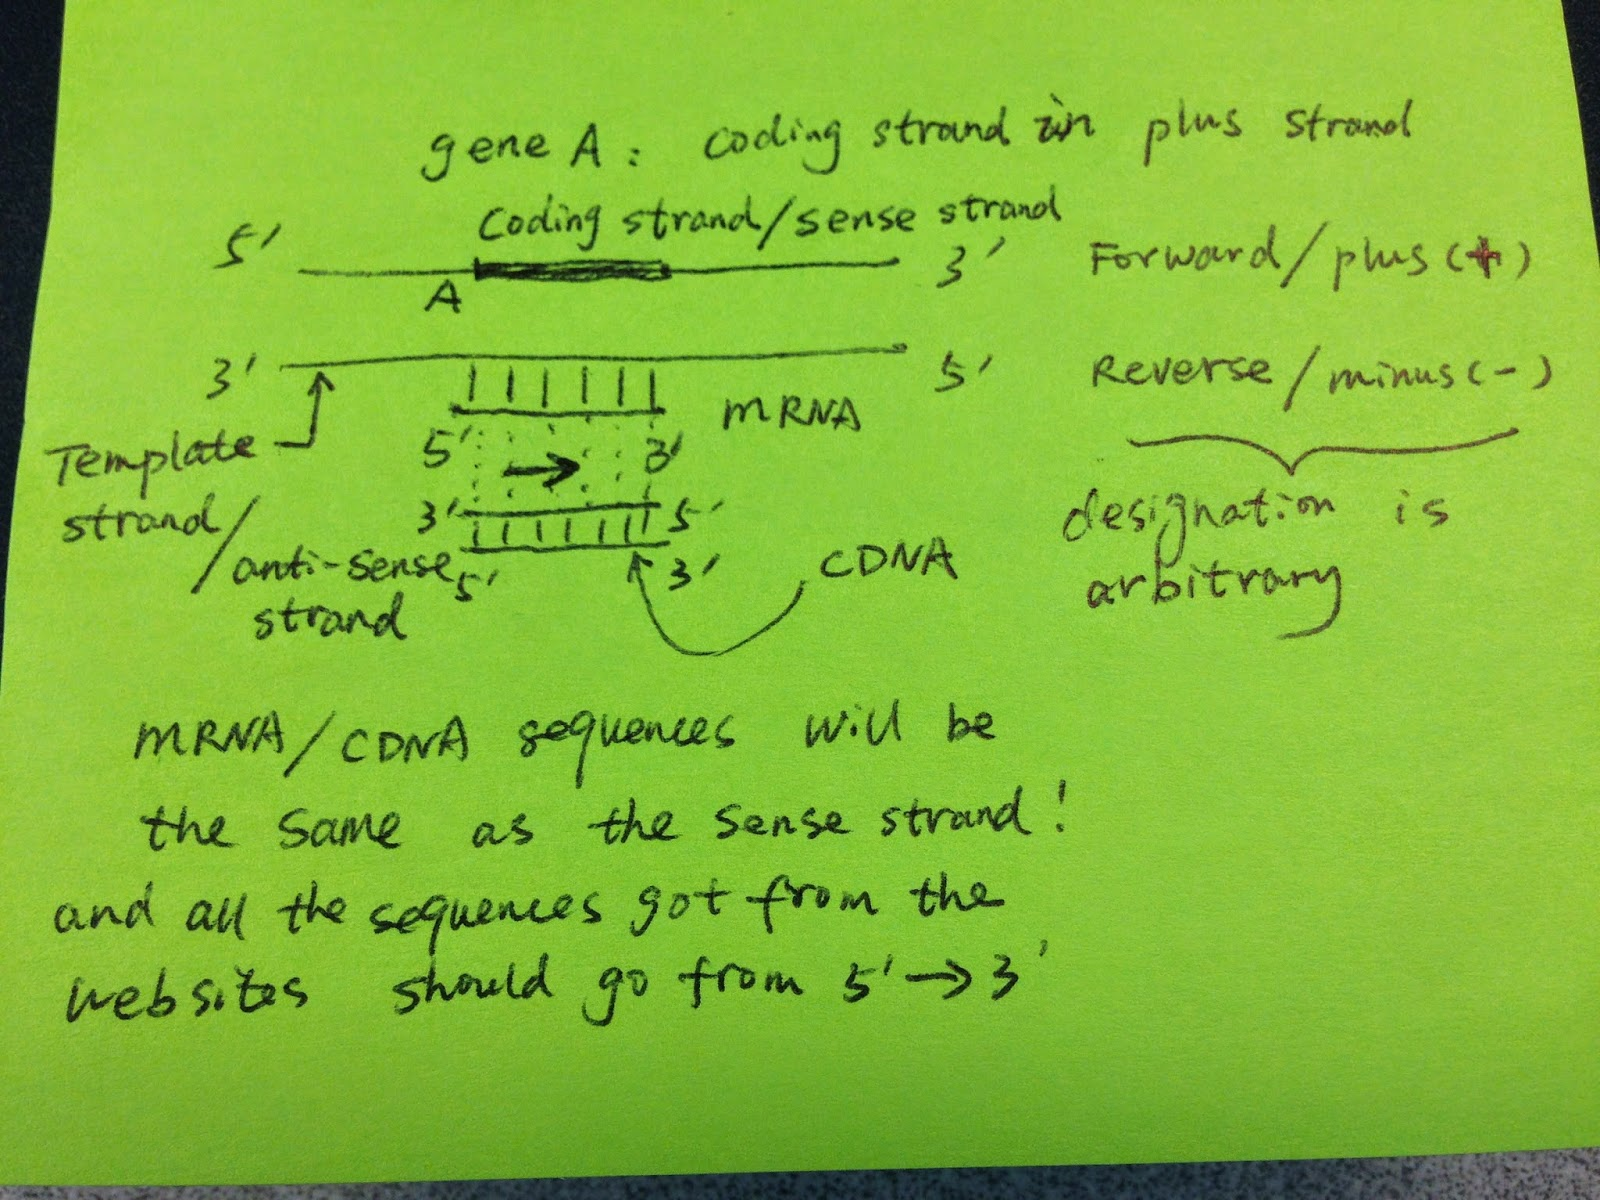
\includegraphics{images/strandness.jpeg}

\hypertarget{basic-operations-with-genomicranges}{%
\subsection{Basic Operations with GenomicRanges}\label{basic-operations-with-genomicranges}}

These operations are commonly used in genomics data analysis to perform tasks such as calculating the length of genomic features, extracting specific regions of interest, and modifying intervals for downstream analysis. \texttt{GenomicRanges} provides a flexible and efficient way to work with genomic intervals, which is essential for tasks like annotation, visualization, and statistical analysis of genomics data.

\hypertarget{calculating-width-of-each-genomic-interval}{%
\subsection{Calculating width of Each Genomic Interval}\label{calculating-width-of-each-genomic-interval}}

Genomic intervals can represent various features in a genome, such as genes, exons, or regulatory regions. Knowing the width of these intervals is crucial when analyzing genomic data. For example, you might want to calculate the size of a gene or measure the distance between two regulatory elements. The \texttt{width()} function helps you obtain this information quickly.

\begin{Shaded}
\begin{Highlighting}[]
\FunctionTok{width}\NormalTok{(gr)}
\end{Highlighting}
\end{Shaded}

\begin{verbatim}
##  [1] 3 3 3 3 3 3 3 3 3 3
\end{verbatim}

This function calculates the width (or length) of each genomic interval in the GenomicRanges object \texttt{gr}. In genomics, the width typically represents the number of base pairs or genomic coordinates covered by each interval.

\hypertarget{start-and-end-positions}{%
\subsection{Start and End Positions}\label{start-and-end-positions}}

Genomic intervals are defined by their start and end positions along a chromosome. These functions allow you to extract these positions, which can be essential for tasks like determining the transcription start site of a gene or identifying the boundaries of a specific genomic region.

\hypertarget{getting-start-position}{%
\subsubsection{Getting start position}\label{getting-start-position}}

\begin{Shaded}
\begin{Highlighting}[]
\FunctionTok{start}\NormalTok{(gr)}
\end{Highlighting}
\end{Shaded}

\begin{verbatim}
##  [1]  1  2  3  4  5  6  7  8  9 10
\end{verbatim}

This function retrieves the starting position (or the leftmost coordinate) of each genomic interval in the \texttt{GenomicRanges} object \texttt{gr}. It tells you where each interval begins along the genome.

\hypertarget{getting-end-position}{%
\subsubsection{Getting end position}\label{getting-end-position}}

\begin{Shaded}
\begin{Highlighting}[]
\FunctionTok{end}\NormalTok{(gr)}
\end{Highlighting}
\end{Shaded}

\begin{verbatim}
##  [1]  3  4  5  6  7  8  9 10 11 12
\end{verbatim}

This function retrieves the ending position (or the rightmost coordinate) of each genomic interval in the \texttt{GenomicRanges} object \texttt{gr}. It tells you where each interval ends along the genome.

\hypertarget{strand-information}{%
\subsection{Strand Information}\label{strand-information}}

In genomics, it's important to know the orientation of genomic features. The strand information (\texttt{+} or \texttt{-}) indicates whether a feature is on the forward (\texttt{+}) or reverse (\texttt{-}) strand of DNA. This can be crucial for understanding gene transcription direction, reading frames, and other biological processes.

\begin{Shaded}
\begin{Highlighting}[]
\FunctionTok{strand}\NormalTok{(gr)}
\end{Highlighting}
\end{Shaded}

\begin{verbatim}
## factor-Rle of length 10 with 1 run
##   Lengths: 10
##   Values :  *
## Levels(3): + - *
\end{verbatim}

Genomic intervals can be associated with a strand information to represent the directionality of a genomic feature. The strand function retrieves the strand information for each interval. The strand can be either ``+'' for the forward strand, ``-'' for the reverse strand, or ``*'' for strand-agnostic intervals.

\hypertarget{shifting-the-genomic-range}{%
\subsection{Shifting the Genomic Range}\label{shifting-the-genomic-range}}

Sometimes, you need to shift genomic intervals to examine neighboring regions. For instance, you might want to find regions that overlap with a gene's promoter, which is typically located upstream of the transcription start site. Shifting intervals allows you to explore nearby genomic areas easily.

\begin{Shaded}
\begin{Highlighting}[]
\NormalTok{gr }\SpecialCharTok{+} \DecValTok{1}
\end{Highlighting}
\end{Shaded}

\begin{verbatim}
## GRanges object with 10 ranges and 0 metadata columns:
##        seqnames    ranges strand
##           <Rle> <IRanges>  <Rle>
##    [1]     chr1       0-4      *
##    [2]     chr1       1-5      *
##    [3]     chr1       2-6      *
##    [4]     chr1       3-7      *
##    [5]     chr1       4-8      *
##    [6]     chr1       5-9      *
##    [7]     chr1      6-10      *
##    [8]     chr1      7-11      *
##    [9]     chr1      8-12      *
##   [10]     chr1      9-13      *
##   -------
##   seqinfo: 1 sequence from an unspecified genome; no seqlengths
\end{verbatim}

This operation demonstrates how you can manipulate the genomic intervals in \texttt{gr}. Here, you are adding 1 to each start \textbf{AND} end position in the intervals, effectively expanding them by one base left and right .

\begin{Shaded}
\begin{Highlighting}[]
\FunctionTok{width}\NormalTok{(gr}\SpecialCharTok{+}\DecValTok{1}\NormalTok{)}
\end{Highlighting}
\end{Shaded}

\begin{verbatim}
##  [1] 5 5 5 5 5 5 5 5 5 5
\end{verbatim}

\hypertarget{subsetting}{%
\subsection{Subsetting}\label{subsetting}}

Genomic data can be extensive, and you often need to focus on specific regions of interest. Subsetting helps you extract only the relevant intervals from a larger dataset. This is especially useful when you want to analyze a particular set of genes or genomic regions.

\begin{Shaded}
\begin{Highlighting}[]
\NormalTok{gr[}\DecValTok{1}\SpecialCharTok{:}\DecValTok{2}\NormalTok{]}
\end{Highlighting}
\end{Shaded}

\begin{verbatim}
## GRanges object with 2 ranges and 0 metadata columns:
##       seqnames    ranges strand
##          <Rle> <IRanges>  <Rle>
##   [1]     chr1       1-3      *
##   [2]     chr1       2-4      *
##   -------
##   seqinfo: 1 sequence from an unspecified genome; no seqlengths
\end{verbatim}

This code subset the GenomicRanges object gr to select the first two intervals. It returns a new GenomicRanges object containing only those intervals.

\hypertarget{flanking-regions}{%
\subsection{Flanking Regions}\label{flanking-regions}}

Imagine you have a specific location in the DNA, and you want to study not only that location but also the regions right before and after it. flank lets you do this. For example, if you're interested in a particular gene, you can use flank to include a bit of the DNA sequence before and after that gene. This helps you see the surrounding context and understand how the gene fits into the bigger picture.

\begin{Shaded}
\begin{Highlighting}[]
\FunctionTok{flank}\NormalTok{(gr, }\DecValTok{2}\NormalTok{)}
\end{Highlighting}
\end{Shaded}

\begin{verbatim}
## GRanges object with 10 ranges and 0 metadata columns:
##        seqnames    ranges strand
##           <Rle> <IRanges>  <Rle>
##    [1]     chr1      -1-0      *
##    [2]     chr1       0-1      *
##    [3]     chr1       1-2      *
##    [4]     chr1       2-3      *
##    [5]     chr1       3-4      *
##    [6]     chr1       4-5      *
##    [7]     chr1       5-6      *
##    [8]     chr1       6-7      *
##    [9]     chr1       7-8      *
##   [10]     chr1       8-9      *
##   -------
##   seqinfo: 1 sequence from an unspecified genome; no seqlengths
\end{verbatim}

\texttt{flank} is useful for tasks like expanding genomic regions of interest to capture nearby regions or creating control regions around known features for downstream analysis. It is commonly used in genomics research to study the context around specific genomic locations.

\hypertarget{resizing}{%
\subsection{Resizing}\label{resizing}}

Think of a situation where you have many different pieces of DNA (intervals), and they're all different lengths. Maybe you want to compare them or count something in each of them. It's easier to work with them if they're all the same size. That's what \texttt{resize} does. It makes sure that all the pieces of DNA are the same length, so you can compare or analyze them more easily.

\begin{Shaded}
\begin{Highlighting}[]
\FunctionTok{resize}\NormalTok{(gr, }\DecValTok{10}\NormalTok{)}
\end{Highlighting}
\end{Shaded}

\begin{verbatim}
## GRanges object with 10 ranges and 0 metadata columns:
##        seqnames    ranges strand
##           <Rle> <IRanges>  <Rle>
##    [1]     chr1      1-10      *
##    [2]     chr1      2-11      *
##    [3]     chr1      3-12      *
##    [4]     chr1      4-13      *
##    [5]     chr1      5-14      *
##    [6]     chr1      6-15      *
##    [7]     chr1      7-16      *
##    [8]     chr1      8-17      *
##    [9]     chr1      9-18      *
##   [10]     chr1     10-19      *
##   -------
##   seqinfo: 1 sequence from an unspecified genome; no seqlengths
\end{verbatim}

\texttt{resize} is used to standardize the length of genomic intervals, which can be useful for comparing or analyzing regions of interest with consistent sizes. It is often applied to ensure that intervals have the same width, making them suitable for various downstream analyses, such as counting reads or comparing features.

\hypertarget{based-and-1-based-coordinate-system}{%
\subsection{0 based and 1 based coordinate system}\label{based-and-1-based-coordinate-system}}

One needs to be aware that there are two genomics coordinate systems: 1 based and 0 based. There is really no mystery between these two. You EITHER count start at 0 OR at 1. However, this can make confusions when analyzing genomic data and one may make mistakes if not keep it in mind. Read \url{https://www.biostars.org/p/84686/}.

The reason that why it matters is that python index starts at 0 while R starts at 1.

Make sure you understand how different bioinformatics format use different coordinate
system.

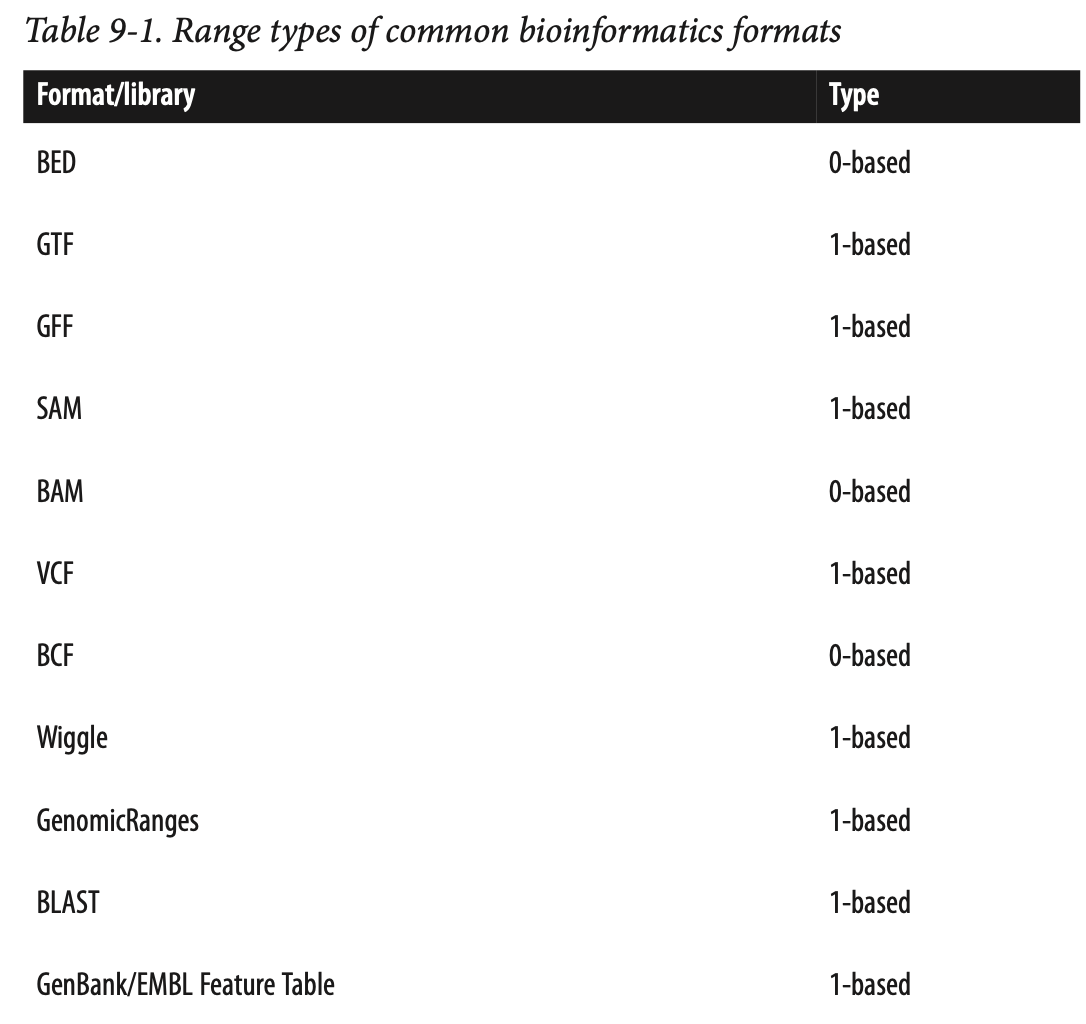
\includegraphics{images/coordinate.png}

\hypertarget{other-packages}{%
\subsection{Other packages}\label{other-packages}}

In genomics research, we often work with genomic data in various formats such as GTF (Gene Transfer Format) and BED files. To facilitate this, we have a few essential packages at our disposal:

\begin{itemize}
\item
  \textbf{AnnotationHub}: This package provides access to a wide range of genome annotations, including GTF files, which are commonly used to represent gene models. These annotations are invaluable for understanding genomic regions and gene structures.
\item
  \textbf{GenomicFeatures}: This package is the powerhouse for working with genomic data in R. It provides functions for creating and manipulating genomic feature objects.
\item
  \textbf{rtracklayer}: This package specializes in reading and handling genomic data files, including BED and GTF files.
\end{itemize}

\hypertarget{accessing-genome-annotations}{%
\subsection{Accessing Genome Annotations}\label{accessing-genome-annotations}}

\begin{quote}
You can check AnnotationHub docs here: \url{https://bioconductor.org/packages/release/bioc/vignettes/AnnotationHub/inst/doc/AnnotationHub.html}
\end{quote}

Genome annotations provide essential information about the location and structure of genes, which is crucial for understanding how genes function and how they are regulated. For example, knowing the coordinates of exons, introns, and promoters allows us to analyze where specific genetic elements are located in the genome.

\begin{Shaded}
\begin{Highlighting}[]
\FunctionTok{library}\NormalTok{(AnnotationHub)}

\CommentTok{\# Initialize the AnnotationHub}
\NormalTok{ah }\OtherTok{\textless{}{-}} \FunctionTok{AnnotationHub}\NormalTok{()}

\CommentTok{\# Query for specific annotations, for example, Homo sapiens (human) in the GRCh37 assembly}
\NormalTok{annotations }\OtherTok{\textless{}{-}}\NormalTok{ AnnotationHub}\SpecialCharTok{::}\FunctionTok{query}\NormalTok{(ah, }\FunctionTok{c}\NormalTok{(}\StringTok{"gtf"}\NormalTok{, }\StringTok{"Homo\_sapiens"}\NormalTok{, }\StringTok{"GRCh37"}\NormalTok{))}

\NormalTok{annotations}
\end{Highlighting}
\end{Shaded}

\begin{verbatim}
## AnnotationHub with 7 records
## # snapshotDate(): 2021-10-20
## # $dataprovider: Ensembl
## # $species: Homo sapiens
## # $rdataclass: GRanges
## # additional mcols(): taxonomyid, genome, description,
## #   coordinate_1_based, maintainer, rdatadateadded, preparerclass, tags,
## #   rdatapath, sourceurl, sourcetype 
## # retrieve records with, e.g., 'object[["AH7558"]]' 
## 
##             title                     
##   AH7558  | Homo_sapiens.GRCh37.70.gtf
##   AH7619  | Homo_sapiens.GRCh37.69.gtf
##   AH7666  | Homo_sapiens.GRCh37.71.gtf
##   AH7726  | Homo_sapiens.GRCh37.72.gtf
##   AH7790  | Homo_sapiens.GRCh37.73.gtf
##   AH8753  | Homo_sapiens.GRCh37.74.gtf
##   AH10684 | Homo_sapiens.GRCh37.75.gtf
\end{verbatim}

\begin{Shaded}
\begin{Highlighting}[]
\CommentTok{\# Select one of the annotations (e.g., GRCh37.gtf)}
\NormalTok{GRCh37.gtf }\OtherTok{\textless{}{-}}\NormalTok{ annotations[[}\StringTok{\textquotesingle{}AH8753\textquotesingle{}}\NormalTok{]]}
\end{Highlighting}
\end{Shaded}

Now, we have a \texttt{GenomicRanges} object called \texttt{GRCh37.gtf}, which contains genomic features from the GRCh37 assembly of the human genome.

\hypertarget{understanding-genomic-biotypes}{%
\subsection{Understanding Genomic Biotypes}\label{understanding-genomic-biotypes}}

Genes in the genome can have different biotypes, indicating their functional roles. We can filter our genomic features based on biotypes, such as ``protein\_coding'' and ``lincRNA.''

Filtering genes by biotype helps us focus on specific classes of genes, such as protein-coding genes, which are involved in producing proteins, or long intergenic non-coding RNAs (lincRNAs), which play regulatory roles.

\begin{Shaded}
\begin{Highlighting}[]
\CommentTok{\# what are the avaiable biotypes}
\FunctionTok{table}\NormalTok{(GRCh37.gtf}\SpecialCharTok{$}\NormalTok{gene\_biotype)}
\end{Highlighting}
\end{Shaded}

\begin{verbatim}
## 
## 3prime_overlapping_ncrna                antisense                IG_C_gene 
##                       63                    28001                      228 
##          IG_C_pseudogene                IG_D_gene                IG_J_gene 
##                       27                      128                       52 
##          IG_J_pseudogene                IG_V_gene          IG_V_pseudogene 
##                        6                      747                      393 
##                  lincRNA                    miRNA                 misc_RNA 
##                    34236                     3361                     2174 
##                  Mt_rRNA                  Mt_tRNA   polymorphic_pseudogene 
##                        2                       22                     3475 
##     processed_pseudogene     processed_transcript           protein_coding 
##                        1                    12720                  2106659 
##               pseudogene                     rRNA           sense_intronic 
##                    44993                      568                     1662 
##        sense_overlapping                   snoRNA                    snRNA 
##                      841                     1549                     2067 
##                TR_C_gene                TR_D_gene                TR_J_gene 
##                       44                        6                      164 
##          TR_J_pseudogene                TR_V_gene          TR_V_pseudogene 
##                        4                      597                       67
\end{verbatim}

\begin{Shaded}
\begin{Highlighting}[]
\CommentTok{\# subset }
\NormalTok{GRCh37.gtf }\OtherTok{\textless{}{-}}\NormalTok{ GRCh37.gtf[GRCh37.gtf}\SpecialCharTok{$}\NormalTok{gene\_biotype }\SpecialCharTok{\%in\%} \FunctionTok{c}\NormalTok{(}\StringTok{"protein\_coding"}\NormalTok{, }\StringTok{"lincRNA"}\NormalTok{)]}
\end{Highlighting}
\end{Shaded}

\hypertarget{creating-a-transcript-database-txdb}{%
\subsection{Creating a Transcript Database (TxDb)}\label{creating-a-transcript-database-txdb}}

\begin{quote}
You can check GenomicFeatures docs here: \url{https://bioconductor.org/packages/release/bioc/vignettes/GenomicFeatures/inst/doc/GenomicFeatures.html}
\end{quote}

To perform more advanced analyses, we'll create a transcript database (\texttt{TxDb}) from our genomic features. A \texttt{TxDb} is a structured database of transcript information, allowing us to efficiently query and retrieve specific genomic elements for analysis.

\begin{Shaded}
\begin{Highlighting}[]
\FunctionTok{library}\NormalTok{(GenomicFeatures)}

\CommentTok{\# Create a TxDb from the filtered genomic features}
\NormalTok{GRCh37.txdb }\OtherTok{\textless{}{-}} \FunctionTok{makeTxDbFromGRanges}\NormalTok{(GRCh37.gtf)}

\NormalTok{GRCh37.txdb}
\end{Highlighting}
\end{Shaded}

\begin{verbatim}
## TxDb object:
## # Db type: TxDb
## # Supporting package: GenomicFeatures
## # Genome: GRCh37
## # Nb of transcripts: 171683
## # Db created by: GenomicFeatures package from Bioconductor
## # Creation time: 2024-06-14 23:15:06 -0400 (Fri, 14 Jun 2024)
## # GenomicFeatures version at creation time: 1.46.5
## # RSQLite version at creation time: 2.3.1
## # DBSCHEMAVERSION: 1.2
\end{verbatim}

\hypertarget{extracting-exons-introns-and-intergenic-regions}{%
\subsection{Extracting Exons, Introns, and Intergenic Regions}\label{extracting-exons-introns-and-intergenic-regions}}

Now that we have our TxDb, we can extract various genomic elements for further analysis.

\hypertarget{exons-by-gene}{%
\subsubsection{Exons by Gene}\label{exons-by-gene}}

Analyzing exons by gene is essential for understanding the coding regions of genes and their splicing patterns. Let's retrieve exons grouped by genes.

\begin{Shaded}
\begin{Highlighting}[]
\NormalTok{exonsByGene }\OtherTok{\textless{}{-}} \FunctionTok{exonsBy}\NormalTok{(GRCh37.txdb, }\StringTok{"gene"}\NormalTok{) }

\CommentTok{\# GRangesList object, a list of GRanges }
\NormalTok{exonsByGene}
\end{Highlighting}
\end{Shaded}

\begin{verbatim}
## GRangesList object of length 30150:
## $ENSG00000000003
## GRanges object with 17 ranges and 2 metadata columns:
##        seqnames            ranges strand |   exon_id       exon_name
##           <Rle>         <IRanges>  <Rle> | <integer>     <character>
##    [1]        X 99883667-99884983      - |    591006 ENSE00001459322
##    [2]        X 99885756-99885863      - |    591007 ENSE00000868868
##    [3]        X 99887482-99887565      - |    591008 ENSE00000401072
##    [4]        X 99887538-99887565      - |    591009 ENSE00001849132
##    [5]        X 99888402-99888536      - |    591010 ENSE00003554016
##    ...      ...               ...    ... .       ...             ...
##   [13]        X 99890555-99890743      - |    591018 ENSE00003662440
##   [14]        X 99891188-99891686      - |    591019 ENSE00001886883
##   [15]        X 99891605-99891803      - |    591020 ENSE00001855382
##   [16]        X 99891790-99892101      - |    591021 ENSE00001863395
##   [17]        X 99894942-99894988      - |    591022 ENSE00001828996
##   -------
##   seqinfo: 265 sequences (1 circular) from GRCh37 genome
## 
## ...
## <30149 more elements>
\end{verbatim}

\hypertarget{merging-all-exons}{%
\subsection{Merging All Exons}\label{merging-all-exons}}

Merging exons (exons can overlap with each other) helps simplify analysis, such as quantifying the overall exonic content of genes. To get a single range representing all exons, we can reduce them.

\begin{Shaded}
\begin{Highlighting}[]
\NormalTok{allExons }\OtherTok{\textless{}{-}} \FunctionTok{exons}\NormalTok{(GRCh37.txdb) }\SpecialCharTok{\%\textgreater{}\%} 
\NormalTok{  GenomicRanges}\SpecialCharTok{::}\FunctionTok{reduce}\NormalTok{()}

\NormalTok{allExons}
\end{Highlighting}
\end{Shaded}

\begin{verbatim}
## GRanges object with 279054 ranges and 0 metadata columns:
##                 seqnames              ranges strand
##                    <Rle>           <IRanges>  <Rle>
##        [1]             1         29554-30039      +
##        [2]             1         30267-30667      +
##        [3]             1         30976-31109      +
##        [4]             1         69091-70008      +
##        [5]             1       160446-160690      +
##        ...           ...                 ...    ...
##   [279050] HSCHR7_1_CTG6 141373867-141374020      -
##   [279051] HSCHR7_1_CTG6 141385280-141385438      -
##   [279052] HSCHR7_1_CTG6 141386361-141386460      -
##   [279053] HSCHR7_1_CTG6 141401359-141401418      -
##   [279054] HSCHR7_1_CTG6 141401689-141401956      -
##   -------
##   seqinfo: 265 sequences (1 circular) from GRCh37 genome
\end{verbatim}

\hypertarget{introns}{%
\subsection{Introns}\label{introns}}

Identifying introns is crucial for studying gene splicing and understanding the non-coding regions within genes. To find intronic regions, we can use the \texttt{intronsByTranscript} function.

\begin{Shaded}
\begin{Highlighting}[]
\NormalTok{introns }\OtherTok{\textless{}{-}} \FunctionTok{intronsByTranscript}\NormalTok{(GRCh37.txdb) }\SpecialCharTok{\%\textgreater{}\%} 
  \FunctionTok{unlist}\NormalTok{() }\SpecialCharTok{\%\textgreater{}\%}
\NormalTok{  GenomicRanges}\SpecialCharTok{::}\FunctionTok{reduce}\NormalTok{()}

\NormalTok{introns}
\end{Highlighting}
\end{Shaded}

\begin{verbatim}
## GRanges object with 185379 ranges and 0 metadata columns:
##                 seqnames              ranges strand
##                    <Rle>           <IRanges>  <Rle>
##        [1]             1         30040-30563      +
##        [2]             1         30668-30975      +
##        [3]             1       160691-161313      +
##        [4]             1       317782-334128      +
##        [5]             1       334298-439466      +
##        ...           ...                 ...    ...
##   [185375] HSCHR7_1_CTG6 141365119-141366086      -
##   [185376] HSCHR7_1_CTG6 141366187-141373866      -
##   [185377] HSCHR7_1_CTG6 141374021-141385279      -
##   [185378] HSCHR7_1_CTG6 141385439-141386360      -
##   [185379] HSCHR7_1_CTG6 141386461-141401688      -
##   -------
##   seqinfo: 265 sequences (1 circular) from GRCh37 genome
\end{verbatim}

\hypertarget{getting-all-genes}{%
\subsection{Getting All Genes}\label{getting-all-genes}}

Having a complete list of genes is essential for various genomics analyses, including differential gene expression studies. Obtaining all genes is straightforward.

\begin{Shaded}
\begin{Highlighting}[]
\NormalTok{allGenes }\OtherTok{\textless{}{-}} \FunctionTok{genes}\NormalTok{(GRCh37.txdb)}

\NormalTok{allGenes}
\end{Highlighting}
\end{Shaded}

\begin{verbatim}
## GRanges object with 30150 ranges and 1 metadata column:
##                                seqnames              ranges strand |
##                                   <Rle>           <IRanges>  <Rle> |
##   ENSG00000000003                     X   99883667-99894988      - |
##   ENSG00000000005                     X   99839799-99854882      + |
##   ENSG00000000419                    20   49551404-49575092      - |
##   ENSG00000000457                     1 169818772-169863408      - |
##   ENSG00000000460                     1 169631245-169823221      + |
##               ...                   ...                 ...    ... .
##   ENSG00000273488                     3 100080031-100080481      + |
##   ENSG00000273490 HSCHR19LRC_LRC_J_CTG1   54693789-54697585      + |
##   ENSG00000273491          HG1308_PATCH 130600118-130603315      + |
##   ENSG00000273492                    21   27543189-27589700      + |
##   ENSG00000273493                     3   58315692-58315845      + |
##                           gene_id
##                       <character>
##   ENSG00000000003 ENSG00000000003
##   ENSG00000000005 ENSG00000000005
##   ENSG00000000419 ENSG00000000419
##   ENSG00000000457 ENSG00000000457
##   ENSG00000000460 ENSG00000000460
##               ...             ...
##   ENSG00000273488 ENSG00000273488
##   ENSG00000273490 ENSG00000273490
##   ENSG00000273491 ENSG00000273491
##   ENSG00000273492 ENSG00000273492
##   ENSG00000273493 ENSG00000273493
##   -------
##   seqinfo: 265 sequences (1 circular) from GRCh37 genome
\end{verbatim}

\hypertarget{promoters}{%
\subsection{Promoters}\label{promoters}}

Promoter regions are critical for understanding gene regulation and identifying potential binding sites for transcription factors. To find promoter regions, typically defined as the region from \texttt{-1kb} to \texttt{+500bp} around the transcription start site (\texttt{TSS}), we can use the promoters function.

\begin{Shaded}
\begin{Highlighting}[]
\NormalTok{promoterRegions }\OtherTok{\textless{}{-}} \FunctionTok{promoters}\NormalTok{(}\FunctionTok{genes}\NormalTok{(GRCh37.txdb), }
                             \AttributeTok{upstream =} \DecValTok{1000}\NormalTok{, }
                             \AttributeTok{downstream =} \DecValTok{500}\NormalTok{)}

\NormalTok{promoterRegions}
\end{Highlighting}
\end{Shaded}

\begin{verbatim}
## GRanges object with 30150 ranges and 1 metadata column:
##                                seqnames              ranges strand |
##                                   <Rle>           <IRanges>  <Rle> |
##   ENSG00000000003                     X   99894489-99895988      - |
##   ENSG00000000005                     X   99838799-99840298      + |
##   ENSG00000000419                    20   49574593-49576092      - |
##   ENSG00000000457                     1 169862909-169864408      - |
##   ENSG00000000460                     1 169630245-169631744      + |
##               ...                   ...                 ...    ... .
##   ENSG00000273488                     3 100079031-100080530      + |
##   ENSG00000273490 HSCHR19LRC_LRC_J_CTG1   54692789-54694288      + |
##   ENSG00000273491          HG1308_PATCH 130599118-130600617      + |
##   ENSG00000273492                    21   27542189-27543688      + |
##   ENSG00000273493                     3   58314692-58316191      + |
##                           gene_id
##                       <character>
##   ENSG00000000003 ENSG00000000003
##   ENSG00000000005 ENSG00000000005
##   ENSG00000000419 ENSG00000000419
##   ENSG00000000457 ENSG00000000457
##   ENSG00000000460 ENSG00000000460
##               ...             ...
##   ENSG00000273488 ENSG00000273488
##   ENSG00000273490 ENSG00000273490
##   ENSG00000273491 ENSG00000273491
##   ENSG00000273492 ENSG00000273492
##   ENSG00000273493 ENSG00000273493
##   -------
##   seqinfo: 265 sequences (1 circular) from GRCh37 genome
\end{verbatim}

\hypertarget{full-genome}{%
\subsection{Full Genome}\label{full-genome}}

Having the entire genome as a single object is useful for genome-wide analyses and visualizations. To represent the entire genome as a GRanges object:

\begin{Shaded}
\begin{Highlighting}[]
\NormalTok{chrom\_granges }\OtherTok{\textless{}{-}} \FunctionTok{as}\NormalTok{(}\FunctionTok{seqinfo}\NormalTok{(GRCh37.txdb), }\StringTok{"GRanges"}\NormalTok{)}
\NormalTok{chrom\_granges}
\end{Highlighting}
\end{Shaded}

\begin{verbatim}
## GRanges object with 265 ranges and 0 metadata columns:
##                        seqnames      ranges strand
##                           <Rle>   <IRanges>  <Rle>
##                1              1 1-249250621      *
##                2              2 1-243199373      *
##                3              3 1-198022430      *
##                4              4 1-191154276      *
##                5              5 1-180915260      *
##              ...            ...         ...    ...
##    HSCHR7_1_CTG6  HSCHR7_1_CTG6 1-159144671      *
##    HSCHR9_1_CTG1  HSCHR9_1_CTG1 1-141228243      *
##   HSCHR9_1_CTG35 HSCHR9_1_CTG35 1-141221627      *
##   HSCHR9_2_CTG35 HSCHR9_2_CTG35 1-141219511      *
##   HSCHR9_3_CTG35 HSCHR9_3_CTG35 1-141224529      *
##   -------
##   seqinfo: 265 sequences (1 circular) from GRCh37 genome
\end{verbatim}

\hypertarget{full-transcriptome}{%
\subsection{Full Transcriptome}\label{full-transcriptome}}

Merging overlapping transcripts simplifies transcript-level analyses and helps identify the full extent of genes. To represent the entire transcriptome, we can merge overlapping features.

\begin{Shaded}
\begin{Highlighting}[]
\NormalTok{collapsed\_tx }\OtherTok{\textless{}{-}}\NormalTok{ GenomicRanges}\SpecialCharTok{::}\FunctionTok{reduce}\NormalTok{(}\FunctionTok{transcripts}\NormalTok{(GRCh37.txdb))}

\CommentTok{\# Set strand information to \textquotesingle{}*\textquotesingle{}}
\FunctionTok{strand}\NormalTok{(collapsed\_tx) }\OtherTok{\textless{}{-}} \StringTok{"*"}
\end{Highlighting}
\end{Shaded}

\hypertarget{intergenic-regions}{%
\subsection{Intergenic Regions}\label{intergenic-regions}}

Intergenic regions often contain important regulatory elements, and identifying them can provide insights into gene regulation. To find regions that are not within any annotated genes, we can use the setdiff function.

\begin{Shaded}
\begin{Highlighting}[]
\NormalTok{intergenicRegions }\OtherTok{\textless{}{-}}\NormalTok{ GenomicRanges}\SpecialCharTok{::}\FunctionTok{setdiff}\NormalTok{(chrom\_granges, collapsed\_tx)}

\NormalTok{intergenicRegions }
\end{Highlighting}
\end{Shaded}

\begin{verbatim}
## GRanges object with 24100 ranges and 0 metadata columns:
##                 seqnames              ranges strand
##                    <Rle>           <IRanges>  <Rle>
##       [1]              1             1-29553      *
##       [2]              1         31110-34553      *
##       [3]              1         36082-69090      *
##       [4]              1         70009-89294      *
##       [5]              1       133567-134900      *
##       ...            ...                 ...    ...
##   [24096]  HSCHR7_1_CTG6 141493731-159144671      *
##   [24097]  HSCHR9_1_CTG1         1-141228243      *
##   [24098] HSCHR9_1_CTG35         1-141221627      *
##   [24099] HSCHR9_2_CTG35         1-141219511      *
##   [24100] HSCHR9_3_CTG35         1-141224529      *
##   -------
##   seqinfo: 265 sequences (1 circular) from GRCh37 genome
\end{verbatim}

\hypertarget{exploring-untranslated-regions-utrs}{%
\subsection{Exploring Untranslated Regions (UTRs)}\label{exploring-untranslated-regions-utrs}}

UTRs play crucial roles in post-transcriptional regulation, and analyzing them can provide insights into gene regulation mechanisms. If you're interested in untranslated regions (UTRs) of genes, you can use functions like \texttt{fiveUTRsByTranscript} and \texttt{threeUTRsByTranscript} provided by the \texttt{GenomicFeatures} package.

\begin{Shaded}
\begin{Highlighting}[]
\CommentTok{\# To get 5\textquotesingle{} UTRs by transcript}
\NormalTok{fiveUTRs }\OtherTok{\textless{}{-}} \FunctionTok{fiveUTRsByTranscript}\NormalTok{(GRCh37.txdb)}

\CommentTok{\# To get 3\textquotesingle{} UTRs by transcript}
\NormalTok{threeUTRs }\OtherTok{\textless{}{-}} \FunctionTok{threeUTRsByTranscript}\NormalTok{(GRCh37.txdb)}
\end{Highlighting}
\end{Shaded}

\hypertarget{conclusion-27}{%
\subsection{Conclusion}\label{conclusion-27}}

In this lesson, we've explored various genomic features and their manipulation using R packages such as \texttt{GenomicFeatures}, \texttt{AnnotationHub}, and \texttt{rtracklayer}. These tools are invaluable for genomics research, allowing you to analyze and interpret genomic data effectively. Whether you're working with ChIP-seq, RNA-seq, or genome annotation, understanding genomic features is essential to uncover the secrets of the genome.

\hypertarget{exploring-cpg-islands-and-shores-in-genomic-data}{%
\section{Exploring CpG Islands and Shores in Genomic Data}\label{exploring-cpg-islands-and-shores-in-genomic-data}}

In this lesson, we will delve into the fascinating world of genomics and learn how to manipulate and analyze genomic data using the powerful tools available in the Bioconductor package. We will specifically focus on CpG islands and their shores, exploring how to extract and analyze these critical genomic features.

\hypertarget{introduction-to-cpg-islands}{%
\subsection{Introduction to CpG Islands}\label{introduction-to-cpg-islands}}

CpG islands are regions of DNA that contain a high frequency of cytosine-guanine (CpG) dinucleotide pairs. These regions are essential for regulating gene expression and have critical roles in various biological processes, including DNA methylation and epigenetic modifications. Analyzing CpG islands can provide valuable insights into gene regulation and genome function.

In this lesson, we will use Bioconductor to fetch CpG island coordinates from the UCSC Genome Browser, extract CpG shores, and perform various genomic operations.

\hypertarget{fetching-cpg-island-coordinates}{%
\subsection{Fetching CpG Island Coordinates}\label{fetching-cpg-island-coordinates}}

CpG islands are critical genomic regions involved in gene regulation and epigenetic modifications. Accessing their coordinates is the first step in understanding their distribution across the genome and their potential functional roles.

Researchers often use CpG island coordinates to investigate gene promoters, identify potential regulatory elements, and study the epigenetic regulation of specific genes in various diseases, including cancer.

To begin, we will retrieve the CpG island coordinates from the UCSC Genome Browser using the \texttt{AnnotationHub} package. CpG islands are available for various species, and in this example, we are using Homo sapiens (human) data.

\begin{Shaded}
\begin{Highlighting}[]
\CommentTok{\# Fetching CpG island coordinates from UCSC Genome Browser}
\FunctionTok{library}\NormalTok{(AnnotationHub)}
\NormalTok{ah }\OtherTok{\textless{}{-}} \FunctionTok{AnnotationHub}\NormalTok{()}

\NormalTok{AnnotationHub}\SpecialCharTok{::}\FunctionTok{query}\NormalTok{(ah, }\FunctionTok{c}\NormalTok{(}\StringTok{"cpg"}\NormalTok{, }\StringTok{"UCSC"}\NormalTok{))}
\end{Highlighting}
\end{Shaded}

\begin{verbatim}
## AnnotationHub with 59 records
## # snapshotDate(): 2021-10-20
## # $dataprovider: UCSC
## # $species: Homo sapiens, Bos taurus, Pan troglodytes, Felis catus, Rattus n...
## # $rdataclass: GRanges
## # additional mcols(): taxonomyid, genome, description,
## #   coordinate_1_based, maintainer, rdatadateadded, preparerclass, tags,
## #   rdatapath, sourceurl, sourcetype 
## # retrieve records with, e.g., 'object[["AH5086"]]' 
## 
##            title      
##   AH5086 | CpG Islands
##   AH5096 | Evo Cpg    
##   AH5204 | CpG Islands
##   AH5227 | Evo Cpg    
##   AH5344 | CpG Islands
##   ...      ...        
##   AH7109 | CpG Islands
##   AH7116 | CpG Islands
##   AH7135 | CpG Islands
##   AH7168 | CpG Islands
##   AH7203 | CpG Islands
\end{verbatim}

use the first entry

\begin{Shaded}
\begin{Highlighting}[]
\NormalTok{cgi }\OtherTok{\textless{}{-}}\NormalTok{ ah[[}\StringTok{"AH5086"}\NormalTok{]]}
\NormalTok{cgi}
\end{Highlighting}
\end{Shaded}

\begin{verbatim}
## GRanges object with 28691 ranges and 1 metadata column:
##                        seqnames        ranges strand |        name
##                           <Rle>     <IRanges>  <Rle> | <character>
##       [1]                  chr1   28736-29810      * |    CpG:_116
##       [2]                  chr1 135125-135563      * |     CpG:_30
##       [3]                  chr1 327791-328229      * |     CpG:_29
##       [4]                  chr1 437152-438164      * |     CpG:_84
##       [5]                  chr1 449274-450544      * |     CpG:_99
##       ...                   ...           ...    ... .         ...
##   [28687]  chr9_gl000201_random   15651-15909      * |     CpG:_30
##   [28688]  chr9_gl000201_random   26397-26873      * |     CpG:_43
##   [28689] chr11_gl000202_random   16284-16540      * |     CpG:_23
##   [28690] chr17_gl000204_random   54686-57368      * |    CpG:_228
##   [28691] chr17_gl000205_random 117501-117801      * |     CpG:_23
##   -------
##   seqinfo: 93 sequences (1 circular) from hg19 genome
\end{verbatim}

We now have the CpG island coordinates stored in the \texttt{cgi} GenomicRanges object.

\hypertarget{defining-cpg-shores}{%
\subsection{Defining CpG Shores}\label{defining-cpg-shores}}

CpG shores are regions located near CpG islands, and they play a crucial role in gene regulation. Defining these shores allows us to explore the regulatory landscape around CpG islands and identify regions of potential interest.

By analyzing CpG shores, researchers can gain insights into how epigenetic modifications in these regions affect gene expression. This knowledge is vital for understanding diseases that involve aberrant gene regulation.

CpG shores are regions located 2000 base pairs upstream and 2000 base pairs downstream of CpG islands. We can use Bioconductor to extract these shores.

\begin{Shaded}
\begin{Highlighting}[]
\CommentTok{\# Extract the shore defined by 2000 bp upstream of CpG islands}
\NormalTok{shore1 }\OtherTok{\textless{}{-}} \FunctionTok{trim}\NormalTok{(}\FunctionTok{flank}\NormalTok{(cgi, }\AttributeTok{width =} \DecValTok{2000}\NormalTok{, }\AttributeTok{start =} \ConstantTok{TRUE}\NormalTok{))}

\CommentTok{\# Extract the shore defined by 2000 bp downstream of CpG islands}
\NormalTok{shore2 }\OtherTok{\textless{}{-}} \FunctionTok{trim}\NormalTok{(}\FunctionTok{flank}\NormalTok{(cgi, }\AttributeTok{width =} \DecValTok{2000}\NormalTok{, }\AttributeTok{start =} \ConstantTok{FALSE}\NormalTok{))}
\end{Highlighting}
\end{Shaded}

\texttt{trim} will trim off the bases that exceed the chromosome ends since we extend 2000 bp
upstream and downstream of the CpG sites. Some CpG sites can be very close to the ends of the chromosomes.

\hypertarget{combining-and-analyzing-cpg-shores}{%
\subsection{Combining and Analyzing CpG Shores}\label{combining-and-analyzing-cpg-shores}}

Combining the upstream and downstream shores and analyzing their overlap with CpG islands helps identify regions with unique genomic characteristics. This step allows researchers to pinpoint areas of interest for further investigation.

Researchers often use this analysis to identify differentially methylated regions (DMRs) associated with specific diseases or conditions. DMRs can serve as biomarkers or potential therapeutic targets.

Now, let's perform some genomic operations on these CpG shores. We'll combine the upstream and downstream shores and identify the features that are present in shores but not in CpG islands (i.e., shores not overlapping with islands).

\begin{Shaded}
\begin{Highlighting}[]
\CommentTok{\# Combine the shores where they overlap}
\NormalTok{shore1\_2 }\OtherTok{\textless{}{-}}\NormalTok{ GenomicRanges}\SpecialCharTok{::}\FunctionTok{reduce}\NormalTok{(}\FunctionTok{c}\NormalTok{(shore1, shore2))}

\CommentTok{\# Extract the features (ranges) that are present in shores only and not in CpG islands}
\NormalTok{cpgi\_shores }\OtherTok{\textless{}{-}}\NormalTok{ GenomicRanges}\SpecialCharTok{::}\FunctionTok{setdiff}\NormalTok{(shore1\_2, cgi)}
\NormalTok{cpgi\_shores}\SpecialCharTok{$}\NormalTok{name }\OtherTok{\textless{}{-}} \FunctionTok{paste}\NormalTok{(}\StringTok{"shore"}\NormalTok{, }\DecValTok{1}\SpecialCharTok{:}\FunctionTok{length}\NormalTok{(cpgi\_shores), }\AttributeTok{sep =} \StringTok{"\_"}\NormalTok{)}

\NormalTok{cpgi\_shores}
\end{Highlighting}
\end{Shaded}

\begin{verbatim}
## GRanges object with 51914 ranges and 1 metadata column:
##                 seqnames        ranges strand |        name
##                    <Rle>     <IRanges>  <Rle> | <character>
##       [1]           chr1   26736-28735      * |     shore_1
##       [2]           chr1   29811-31810      * |     shore_2
##       [3]           chr1 133125-135124      * |     shore_3
##       [4]           chr1 135564-137563      * |     shore_4
##       [5]           chr1 325791-327790      * |     shore_5
##       ...            ...           ...    ... .         ...
##   [51910] chrUn_gl000241   37274-39273      * | shore_51910
##   [51911] chrUn_gl000242   10843-12842      * | shore_51911
##   [51912] chrUn_gl000242   13100-15099      * | shore_51912
##   [51913] chrUn_gl000243   28420-30419      * | shore_51913
##   [51914] chrUn_gl000243   30716-32715      * | shore_51914
##   -------
##   seqinfo: 93 sequences (1 circular) from hg19 genome
\end{verbatim}

Now, \texttt{cpgi\_shores} contains the \texttt{GenomicRanges} object representing CpG shores, and each shore is labeled with a unique name.

\hypertarget{conclusion-28}{%
\subsection{Conclusion}\label{conclusion-28}}

In this lesson, we've explored the powerful capabilities of the Bioconductor package for working with genomic data. We've fetched CpG island coordinates, extracted CpG shores, and performed genomic operations to identify regions of interest. These techniques are fundamental for researchers and bioinformaticians working with genomics data to unravel the mysteries of the genome.

If you're interested in diving deeper into genomics analysis, consider exploring the tutorials provided by Bioconductor on their website. They offer a wealth of knowledge and resources to help you harness the full potential of genomic data analysis.

\hypertarget{real-world-applications-chip-seq}{%
\section{Real-World Applications: ChIP-seq}\label{real-world-applications-chip-seq}}

Understanding genomic features is crucial for various genomics tasks, including:

\begin{itemize}
\item
  ChIP-seq Analysis: You can use these genomic ranges to determine how many ChIP-seq peaks fall into promoters, exons, introns, or intergenic regions, helping you interpret the functional significance of your data.
\item
  RNA-seq Analysis: Identifying which exons are covered by RNA-seq reads and counting reads in each exon allows you to quantify gene expression accurately.
\item
  Functional Genomics: Investigating the genomic context of genes helps in understanding their regulatory elements, including promoters and enhancers.
\item
  Genome Annotation: These tools are essential for creating comprehensive annotations of genomes, enabling researchers to understand gene structures and functions.
\end{itemize}

\hypertarget{read-in-peak-file}{%
\subsubsection{read in peak file}\label{read-in-peak-file}}

\hypertarget{identify-promoters-that-overlap-with-the-peaks}{%
\subsection{Identify promoters that overlap with the peaks}\label{identify-promoters-that-overlap-with-the-peaks}}

\hypertarget{use-the-chipseeker-package}{%
\subsection{use the ChIPseeker package}\label{use-the-chipseeker-package}}

\hypertarget{analyzing-and-visualizing-genomic-data}{%
\section{Analyzing and Visualizing Genomic Data}\label{analyzing-and-visualizing-genomic-data}}

In this lesson, we will explore several essential tools and techniques used in genomics research, including \texttt{GEOquery} for data retrieval, gene ID conversion using \texttt{biomaRt} and \texttt{org.Hs.eg.db}, and visualization with \texttt{ComplexHeatmap}. These tools are commonly used in genomics to analyze and visualize gene expression data. We will briefly mention \texttt{DESeq2} for differential expression analysis.

\hypertarget{deseq2}{%
\subsection{DESeq2}\label{deseq2}}

\begin{quote}
You can explore docs here: \url{https://bioconductor.org/packages/release/bioc/vignettes/DESeq2/inst/doc/DESeq2.html}
\end{quote}

\texttt{DESeq2} is a powerful Bioconductor package used for differential expression analysis. It is particularly helpful when working with RNA-seq data. This tool helps identify genes that are differentially expressed under different conditions. The tutorial on Bioconductor is very comprehensive and I will leave the students to read by themselves. We will use it in our final project.

\hypertarget{geoquery}{%
\subsection{GEOquery}\label{geoquery}}

\begin{quote}
You can explore docs here: \url{https://bioconductor.org/packages/release/bioc/vignettes/GEOquery/inst/doc/GEOquery.html}
\end{quote}

\texttt{GEOquery} is a valuable R package for downloading and importing gene expression data directly from public repositories such as the Gene Expression Omnibus (GEO).

\begin{Shaded}
\begin{Highlighting}[]
\CommentTok{\# Loading the GEOquery library}
\FunctionTok{library}\NormalTok{(GEOquery)}

\CommentTok{\# Downloading and importing data from GEO}
\NormalTok{GSE197576 }\OtherTok{\textless{}{-}} \FunctionTok{getGEO}\NormalTok{(}\AttributeTok{GEO =} \StringTok{"GSE197576"}\NormalTok{, }\AttributeTok{GSEMatrix =} \ConstantTok{TRUE}\NormalTok{, }\AttributeTok{destdir =} \StringTok{"\textasciitilde{}/Downloads"}\NormalTok{)}

\NormalTok{GSE197576}
\end{Highlighting}
\end{Shaded}

\begin{verbatim}
## $GSE197576_series_matrix.txt.gz
## ExpressionSet (storageMode: lockedEnvironment)
## assayData: 0 features, 12 samples 
##   element names: exprs 
## protocolData: none
## phenoData
##   sampleNames: GSM5920759 GSM5920760 ... GSM5920770 (12 total)
##   varLabels: title geo_accession ... tissue:ch1 (43 total)
##   varMetadata: labelDescription
## featureData: none
## experimentData: use 'experimentData(object)'
##   pubMedIds: 35487218 
## Annotation: GPL18573
\end{verbatim}

\begin{Shaded}
\begin{Highlighting}[]
\CommentTok{\# Accessing expression data}
\FunctionTok{exprs}\NormalTok{(GSE197576}\SpecialCharTok{$}\NormalTok{GSE197576\_series\_matrix.txt.gz)}
\end{Highlighting}
\end{Shaded}

\begin{verbatim}
##      GSM5920759 GSM5920760 GSM5920761 GSM5920762 GSM5920763 GSM5920764
##      GSM5920765 GSM5920766 GSM5920767 GSM5920768 GSM5920769 GSM5920770
\end{verbatim}

In this example, it returns an empty \texttt{ExpressionSet} object. We used \texttt{exprs} to return
the matrix but it has no features. You may try a different GEO accession.

\texttt{GEOquery} simplifies the process of retrieving gene expression data from public repositories like GEO. Researchers use it to access valuable datasets for their studies.

\hypertarget{converting-gene-ids}{%
\subsection{Converting Gene IDs}\label{converting-gene-ids}}

In genomics research, integrating data from various sources often involves working with different gene identifier systems. Converting gene IDs is a crucial step to harmonize and standardize data for downstream analysis. Here, we discuss two commonly used methods, biomaRt and org.Hs.eg.db, and explain why these tasks are essential in a researcher's environment.

\hypertarget{using-biomart}{%
\subsubsection{Using biomaRt}\label{using-biomart}}

\begin{quote}
You can explore docs here: \url{https://bioconductor.org/packages/release/bioc/vignettes/biomaRt/inst/doc/accessing_ensembl.html}
\end{quote}

Converting gene IDs using \texttt{biomaRt} is essential for mapping Ensembl gene IDs to more recognizable gene symbols and associated information.

\begin{Shaded}
\begin{Highlighting}[]
\FunctionTok{library}\NormalTok{(biomaRt)}
\NormalTok{ensembl }\OtherTok{\textless{}{-}} \FunctionTok{useMart}\NormalTok{(}\StringTok{"ensembl"}\NormalTok{, }\AttributeTok{dataset =} \StringTok{"hsapiens\_gene\_ensembl"}\NormalTok{)}

\NormalTok{gene\_info }\OtherTok{\textless{}{-}} \FunctionTok{getBM}\NormalTok{(}\AttributeTok{attributes =} \FunctionTok{c}\NormalTok{(}\StringTok{"ensembl\_gene\_id"}\NormalTok{, }\StringTok{"gene\_biotype"}\NormalTok{,}
                                  \StringTok{"chromosome\_name"}\NormalTok{, }\StringTok{"hgnc\_symbol"}\NormalTok{),}
                   \AttributeTok{filters =} \StringTok{"ensembl\_gene\_id"}\NormalTok{, }
                   \AttributeTok{values =} \FunctionTok{c}\NormalTok{(}\StringTok{"ENSG00000164307"}\NormalTok{), }
                   \AttributeTok{mart =}\NormalTok{ ensembl)}
\FunctionTok{print}\NormalTok{(gene\_info)}
\end{Highlighting}
\end{Shaded}

\begin{verbatim}
##   ensembl_gene_id   gene_biotype chromosome_name hgnc_symbol
## 1 ENSG00000164307 protein_coding               5       ERAP1
\end{verbatim}

\hypertarget{using-org.hs.eg.db}{%
\subsubsection{Using org.Hs.eg.db}\label{using-org.hs.eg.db}}

\begin{quote}
You can explore docs here: \url{https://bioconductor.org/packages/release/data/annotation/html/org.Hs.eg.db.html}
\end{quote}

Mapping ENTREZIDs to official gene symbols using \texttt{org.Hs.eg.db} is crucial for researchers working with gene expression data.

Why Researchers Do This:

\begin{itemize}
\item
  Consistency in Annotation: ENTREZIDs are a widely accepted and consistent gene identifier system. Mapping other identifiers to ENTREZIDs ensures that gene information is uniform and can be compared across different studies.
\item
  Integration with Other Databases: Many databases and tools use ENTREZIDs (e.g., the KEGG pathway database) as a standard for gene annotation. Converting identifiers to ENTREZIDs facilitates seamless integration with these resources.
\item
  Gene Symbol Mapping: Once converted to ENTREZIDs, researchers can efficiently map these to official gene symbols, providing meaningful and interpretable gene names for further analysis and reporting.
\end{itemize}

\begin{Shaded}
\begin{Highlighting}[]
\CommentTok{\# Loading the org.Hs.eg.db library}
\FunctionTok{library}\NormalTok{(org.Hs.eg.db)}
\FunctionTok{library}\NormalTok{(TxDb.Hsapiens.UCSC.hg19.knownGene)}

\CommentTok{\# Accessing gene information}
\NormalTok{hg19\_genes }\OtherTok{\textless{}{-}} \FunctionTok{genes}\NormalTok{(TxDb.Hsapiens.UCSC.hg19.knownGene)}

\CommentTok{\# Mapping ENTREZIDs to official gene symbols}
\NormalTok{map }\OtherTok{\textless{}{-}}\NormalTok{ AnnotationDbi}\SpecialCharTok{::}\FunctionTok{select}\NormalTok{(org.Hs.eg.db, }\AttributeTok{keys =}\NormalTok{ hg19\_genes}\SpecialCharTok{$}\NormalTok{gene\_id, }
                            \AttributeTok{columns =} \StringTok{"SYMBOL"}\NormalTok{, }\AttributeTok{keytype =} \StringTok{"ENTREZID"}\NormalTok{)}

\FunctionTok{head}\NormalTok{(map, }\AttributeTok{n =} \DecValTok{10}\NormalTok{)}
\end{Highlighting}
\end{Shaded}

\begin{verbatim}
##     ENTREZID     SYMBOL
## 1          1       A1BG
## 2         10       NAT2
## 3        100        ADA
## 4       1000       CDH2
## 5      10000       AKT3
## 6  100008586    GAGE12F
## 7  100009676 ZBTB11-AS1
## 8      10001       MED6
## 9      10002      NR2E3
## 10     10003    NAALAD2
\end{verbatim}

In genomics research, this type of mapping is essential when you have data that uses ENTREZIDs, and you want to work with more interpretable gene symbols for analysis or visualization. It allows you to associate gene identifiers with their official names, making the data more understandable and facilitating downstream analyses and interpretation.

\hypertarget{complexheatmap}{%
\subsection{ComplexHeatmap}\label{complexheatmap}}

\begin{quote}
You can explore docs here: \url{https://bioconductor.org/packages/release/bioc/html/ComplexHeatmap.html}
\end{quote}

Visualizing gene expression data is a crucial step in genomics research because it helps researchers gain insights into how genes are expressed under different conditions or in various samples. \texttt{ComplexHeatmap} is a versatile R package that serves as an artistic palette for creating intricate and informative heatmaps. Here's why visualizing gene expression data using \texttt{ComplexHeatmap} is essential:

\begin{enumerate}
\def\labelenumi{\arabic{enumi}.}
\item
  Identify Expression Patterns: Gene expression data often involve a large number of genes and samples. Heatmaps allow you to quickly identify patterns in gene expression, such as clusters of genes with similar expression profiles. This can reveal groups of genes that are co-regulated or have similar functions.
\item
  Visualize Differential Expression: When comparing gene expression between different conditions or treatments (e.g., healthy vs.~diseased tissue), heatmaps can highlight genes that are significantly upregulated or downregulated. This visualization aids in pinpointing genes of interest for further investigation.
\item
  Sample Relationships: Heatmaps also help in understanding the relationships between samples. For example, you can identify outliers, detect batch effects, or confirm the consistency of replicates by examining how samples cluster based on their expression profiles.
\item
  Publication-Ready Figures: ComplexHeatmap generates high-quality heatmap images that are suitable for inclusion in research papers and presentations. It provides the ability to export heatmaps in various formats (e.g., PDF, PNG) for easy sharing and publication.
\item
  Interactive Exploration: In addition to static heatmaps, \href{https://www.bioconductor.org/packages/release/bioc/html/InteractiveComplexHeatmap.html}{InteractiveComplexHeatmap} from the same author supports interactive exploration. You can zoom in on specific sections of the heatmap, hover over cells to view gene names or expression values, and provide interactive tools for your audience to explore the data themselves.
\end{enumerate}

Le's go through an example by simulating a count matrix from a gene expression experiment:

\begin{Shaded}
\begin{Highlighting}[]
\FunctionTok{library}\NormalTok{(ComplexHeatmap)}

\FunctionTok{set.seed}\NormalTok{(}\DecValTok{123}\NormalTok{)}

\CommentTok{\# Parameters for the negative binomial distribution}
\NormalTok{size\_parameter }\OtherTok{\textless{}{-}} \DecValTok{3} \CommentTok{\# Size parameter (dispersion)}
\NormalTok{mean\_parameter }\OtherTok{\textless{}{-}} \DecValTok{10}  \CommentTok{\# Mean parameter}

\CommentTok{\# Number of genes (rows) and samples (columns)}
\NormalTok{num\_genes }\OtherTok{\textless{}{-}} \DecValTok{10}
\NormalTok{num\_samples }\OtherTok{\textless{}{-}} \DecValTok{20}

\CommentTok{\# Simulate a count table with negative binomial distribution}
\NormalTok{expr\_data }\OtherTok{\textless{}{-}} \FunctionTok{matrix}\NormalTok{(}\FunctionTok{rnbinom}\NormalTok{(num\_genes }\SpecialCharTok{*}\NormalTok{ num\_samples, }
                            \AttributeTok{size =}\NormalTok{ size\_parameter, }
                            \AttributeTok{mu =}\NormalTok{ mean\_parameter), }
                    \AttributeTok{nrow =}\NormalTok{ num\_genes, }
                    \AttributeTok{ncol =}\NormalTok{ num\_samples)}
\end{Highlighting}
\end{Shaded}

check the quantiles of the data. This is important because we need to know the
ranges of the data so we can map the values to color.

\begin{Shaded}
\begin{Highlighting}[]
\FunctionTok{quantile}\NormalTok{(expr\_data, }\FunctionTok{c}\NormalTok{(}\DecValTok{0}\NormalTok{, }\FloatTok{0.2}\NormalTok{, }\FloatTok{0.5}\NormalTok{, }\FloatTok{0.8}\NormalTok{, }\DecValTok{1}\NormalTok{))}
\end{Highlighting}
\end{Shaded}

\begin{verbatim}
##   0%  20%  50%  80% 100% 
##    0    4    9   14   31
\end{verbatim}

Map the color to the values

\begin{Shaded}
\begin{Highlighting}[]
\NormalTok{color\_map}\OtherTok{\textless{}{-}}\NormalTok{ circlize}\SpecialCharTok{::}\FunctionTok{colorRamp2}\NormalTok{(}\FunctionTok{c}\NormalTok{(}\DecValTok{0}\NormalTok{, }\DecValTok{9}\NormalTok{, }\DecValTok{25}\NormalTok{), }\FunctionTok{c}\NormalTok{(}\StringTok{"blue"}\NormalTok{, }\StringTok{"white"}\NormalTok{, }\StringTok{"red"}\NormalTok{))}
\end{Highlighting}
\end{Shaded}

Any value beyond 25 will be mapped to the same intensity of redness.

Make the heatmap:

\begin{Shaded}
\begin{Highlighting}[]
\FunctionTok{Heatmap}\NormalTok{(expr\_data, }\AttributeTok{col=}\NormalTok{color\_map, }\AttributeTok{name =} \StringTok{"gene\_expression"}\NormalTok{)}
\end{Highlighting}
\end{Shaded}

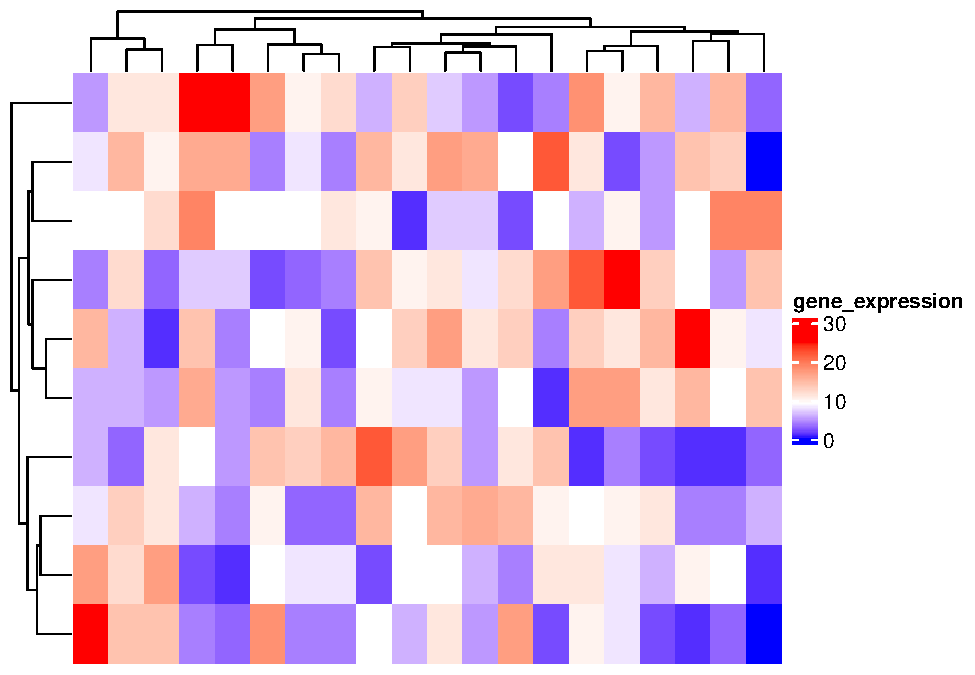
\includegraphics{10_Introduction_to_BioConductor_files/figure-latex/unnamed-chunk-39-1.pdf}

By default, it will cluster both the rows and columns.

Let's see how it looks if we change the color mapping

\begin{Shaded}
\begin{Highlighting}[]
\NormalTok{color\_map2}\OtherTok{\textless{}{-}}\NormalTok{ circlize}\SpecialCharTok{::}\FunctionTok{colorRamp2}\NormalTok{(}\FunctionTok{c}\NormalTok{(}\DecValTok{0}\NormalTok{, }\DecValTok{25}\NormalTok{, }\DecValTok{31}\NormalTok{), }\FunctionTok{c}\NormalTok{(}\StringTok{"blue"}\NormalTok{, }\StringTok{"white"}\NormalTok{, }\StringTok{"red"}\NormalTok{))}
\FunctionTok{Heatmap}\NormalTok{(expr\_data, }\AttributeTok{col=}\NormalTok{color\_map2, }\AttributeTok{name =} \StringTok{"gene\_expression"}\NormalTok{)}
\end{Highlighting}
\end{Shaded}

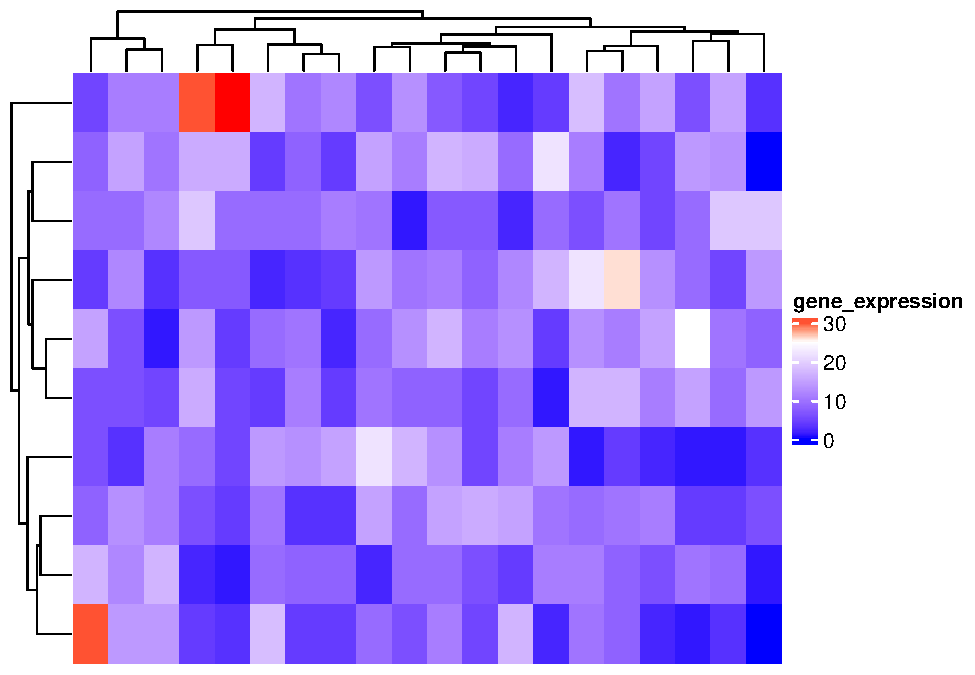
\includegraphics{10_Introduction_to_BioConductor_files/figure-latex/unnamed-chunk-40-1.pdf}
Now, we see very fewer red cells, but the underlying data is the same! How you map the values to color makes a big difference on how the heatmap look. Note the legend reflects our changes in the color mapping.

We will use it again in the next section.

\hypertarget{conclusion-29}{%
\subsection{Conclusion}\label{conclusion-29}}

This lesson has provided an overview of essential tools and techniques used in genomics research. We have explored the following key topics:

\begin{itemize}
\item
  \texttt{DESeq2}: We learned about DESeq2 for differential expression analysis, which is crucial for identifying genes that are differentially expressed under different conditions, such as in disease versus healthy states.
\item
  \texttt{GEOquery}: We discussed how to retrieve gene expression data from public repositories like GEO using the GEOquery package. Accessing publicly available datasets is a valuable resource for genomics research.
\item
  Gene ID Conversion: We covered two methods, \texttt{biomaRt} and \texttt{org.Hs.eg.db}, for converting gene IDs. This step is essential for integrating data from various sources and ensuring consistent gene identification.
\item
  \texttt{ComplexHeatmap}: We explored the \texttt{ComplexHeatmap} package, a powerful tool for visualizing gene expression data through heatmaps. Visualization aids in identifying patterns and trends in large genomic datasets.
\end{itemize}

These tools and techniques are indispensable for genomics researchers, enabling them to analyze, integrate, and visualize genomic data effectively. By mastering these skills, researchers can gain valuable insights into gene expression patterns, biological processes, and potential biomarkers for various conditions and diseases.

\hypertarget{real-world-example---tcga-analysis}{%
\section{Real-World Example - TCGA Analysis}\label{real-world-example---tcga-analysis}}

In this lesson, we will explore a real-world example of analyzing cancer genomics data from \href{https://www.cancer.gov/ccg/research/genome-sequencing/tcga}{The Cancer Genome Atlas (TCGA)} project. TCGA is one of the largest and most renowned cancer sequencing projects, providing access to a wealth of genomic data from various cancer types. We will use R and several bioinformatics packages to download raw RNA-seq counts for 33 different cancer types, convert them to TPM (transcripts per million), and visualize the data in a heatmap.

\hypertarget{introduction-to-tcga}{%
\subsection{Introduction to TCGA}\label{introduction-to-tcga}}

The Cancer Genome Atlas (TCGA) project is a groundbreaking initiative that has sequenced approximately 10,000 treatment-naive tumors across 33 different cancer types. It has generated a diverse range of data types, including whole-exome sequencing, whole-genome sequencing, copy-number variation analysis (SNP arrays), bulk RNA-seq, protein expression data (Reverse-Phase Protein Array), and DNA methylation profiles. TCGA has significantly contributed to our understanding of cancer biology and has opened up new avenues for cancer research.

\hypertarget{why-analyze-tcga-data}{%
\subsection{Why Analyze TCGA Data?}\label{why-analyze-tcga-data}}

Analyzing TCGA data can provide valuable insights into the molecular basis of cancer. Researchers can use this data to identify potential biomarkers, discover novel therapeutic targets, and gain a deeper understanding of the genetic alterations associated with specific cancer types. Moreover, TCGA data is freely accessible, making it a valuable resource for the scientific community.

\hypertarget{getting-started-1}{%
\subsection{Getting Started}\label{getting-started-1}}

We will use the \href{https://bioconductor.org/packages/release/bioc/html/recount3.html}{\texttt{recount3}} package to access TCGA data. \texttt{recount3} is an online resource that provides RNA-seq gene, exon, and exon-exon junction counts, along with coverage bigWig files for thousands of studies in both human and mouse. It represents the third generation of the \href{https://rna.recount.bio/}{ReCount} project.

\hypertarget{step-1-install-and-load-required-packages}{%
\subsection{Step 1: Install and Load Required Packages}\label{step-1-install-and-load-required-packages}}

\begin{Shaded}
\begin{Highlighting}[]
\CommentTok{\# Install the recount3 package if not already installed}
\CommentTok{\# BiocManager::install("recount3")}

\CommentTok{\# Load necessary libraries}
\FunctionTok{library}\NormalTok{(recount3)}
\FunctionTok{library}\NormalTok{(purrr)}
\FunctionTok{library}\NormalTok{(dplyr)}
\FunctionTok{library}\NormalTok{(ggplot2)}
\end{Highlighting}
\end{Shaded}

\begin{itemize}
\item
  recount3: This package is crucial for accessing TCGA data. It allows us to retrieve RNA-seq gene counts and other genomic information from the TCGA project.
\item
  purrr: The purrr package is used for functional programming in R. We use it to apply functions to elements of a list, which is particularly useful for handling multiple datasets or projects.
\item
  dplyr: dplyr is a powerful package for data manipulation. It helps us filter and process data efficiently, making it easier to work with large datasets like TCGA.
\item
  ggplot2: For data visualization, we use the ggplot2 package. It allows us to create high-quality graphs and plots, which can be essential for presenting our findings.
\end{itemize}

By loading these packages, we ensure that we have access to the tools needed to analyze and visualize TCGA data effectively.

\hypertarget{step-2-retrieve-tcga-project-information}{%
\subsection{Step 2: Retrieve TCGA Project Information}\label{step-2-retrieve-tcga-project-information}}

Let's fetch information about available TCGA projects. TCGA encompasses a wide range of cancer types and studies. We filter the projects to focus only on those that originate from TCGA data sources.

\begin{Shaded}
\begin{Highlighting}[]
\CommentTok{\# Get information about available TCGA projects}
\NormalTok{human\_projects }\OtherTok{\textless{}{-}} \FunctionTok{available\_projects}\NormalTok{()}

\CommentTok{\# Filter projects that are from TCGA data sources}
\NormalTok{tcga\_info }\OtherTok{\textless{}{-}} \FunctionTok{subset}\NormalTok{(}
\NormalTok{    human\_projects,}
\NormalTok{    file\_source }\SpecialCharTok{==} \StringTok{"tcga"} \SpecialCharTok{\&}\NormalTok{ project\_type }\SpecialCharTok{==} \StringTok{"data\_sources"}
\NormalTok{)}


\FunctionTok{head}\NormalTok{(tcga\_info)}
\end{Highlighting}
\end{Shaded}

\begin{verbatim}
##      project organism file_source      project_home project_type n_samples
## 8710     ACC    human        tcga data_sources/tcga data_sources        79
## 8711    BLCA    human        tcga data_sources/tcga data_sources       433
## 8712    BRCA    human        tcga data_sources/tcga data_sources      1256
## 8713    CESC    human        tcga data_sources/tcga data_sources       309
## 8714    CHOL    human        tcga data_sources/tcga data_sources        45
## 8715    COAD    human        tcga data_sources/tcga data_sources       546
\end{verbatim}

This step is essential to identify the relevant projects and data sources within TCGA. By narrowing our focus to TCGA data sources, we ensure that we are working with the specific datasets we need for our analysis.

\hypertarget{step-3-create-a-rangedsummarizedexperiment-object}{%
\subsection{Step 3: Create a RangedSummarizedExperiment Object}\label{step-3-create-a-rangedsummarizedexperiment-object}}

Now that we have identified the TCGA data sources of interest, we proceed to create a data structure called a \href{https://www.bioconductor.org/packages/devel/bioc/vignettes/SummarizedExperiment/inst/doc/SummarizedExperiment.html}{\texttt{RangedSummarizedExperiment}} object. This object allows us to efficiently organize and work with genomic data, including RNA-seq counts.

\begin{Shaded}
\begin{Highlighting}[]
\CommentTok{\# Create a list of RangedSummarizedExperiment objects}
\NormalTok{proj\_info }\OtherTok{\textless{}{-}}\NormalTok{ purrr}\SpecialCharTok{::}\FunctionTok{map}\NormalTok{(}\FunctionTok{seq}\NormalTok{(}\FunctionTok{nrow}\NormalTok{(tcga\_info)), }\SpecialCharTok{\textasciitilde{}}\NormalTok{tcga\_info[.x, ])}
\NormalTok{rse\_tcga }\OtherTok{\textless{}{-}}\NormalTok{ purrr}\SpecialCharTok{::}\FunctionTok{map}\NormalTok{(proj\_info, }\SpecialCharTok{\textasciitilde{}}\FunctionTok{create\_rse}\NormalTok{(.x))}
\end{Highlighting}
\end{Shaded}

Here, we create a list of \texttt{RangedSummarizedExperiment} objects, one for each project within TCGA. These objects will serve as containers for the gene expression data, making it easier to manipulate and analyze the information.

The first time you use \texttt{recount3}, it will ask:

\begin{quote}
/Users/tommytang/Library/Caches/org.R-project.R/R/recount3 does not exist, create directory? (yes/no): yes
\end{quote}

\texttt{rse\_tcga} is a list of \texttt{RangedSummarizedExperimentobject}, let's take a look at one of them. \texttt{RangedSummarizedExperiment} is a child of the \texttt{SummarizedExperiment}.

\begin{Shaded}
\begin{Highlighting}[]
\NormalTok{rse\_tcga[[}\DecValTok{1}\NormalTok{]]}
\end{Highlighting}
\end{Shaded}

\begin{verbatim}
## class: RangedSummarizedExperiment 
## dim: 63856 79 
## metadata(8): time_created recount3_version ... annotation recount3_url
## assays(1): raw_counts
## rownames(63856): ENSG00000278704.1 ENSG00000277400.1 ...
##   ENSG00000182484.15_PAR_Y ENSG00000227159.8_PAR_Y
## rowData names(10): source type ... havana_gene tag
## colnames(79): 43e715bf-28d9-4b5e-b762-8cd1b69a430e
##   1a5db9fc-2abd-4e1b-b5ef-b1cf5e5f3872 ...
##   a08b85ea-d1e7-4b77-8dec-36294305b9f7
##   aa2d53e5-d389-4332-9dd5-a736052e48f8
## colData names(937): rail_id external_id ... recount_seq_qc.errq
##   BigWigURL
\end{verbatim}

\hypertarget{step-4-explore-tcga-data}{%
\subsection{Step 4: Explore TCGA Data}\label{step-4-explore-tcga-data}}

With our \texttt{RangedSummarizedExperiment} objects in place, we can now explore the TCGA data in more detail. Let's look at three aspects: gene counts, gene information, and metadata.

\hypertarget{gene-counts}{%
\subsubsection{Gene Counts}\label{gene-counts}}

We start by examining the raw RNA-seq counts, which represent how many times each gene was sequenced in each sample.

\begin{Shaded}
\begin{Highlighting}[]
\CommentTok{\# Access raw gene counts from one RangedSummarizedExperiment object}
\NormalTok{raw\_counts }\OtherTok{\textless{}{-}}\NormalTok{ rse\_tcga[[}\DecValTok{1}\NormalTok{]]}\SpecialCharTok{@}\NormalTok{assays}\SpecialCharTok{@}\NormalTok{data}\SpecialCharTok{$}\NormalTok{raw\_counts[}\DecValTok{1}\SpecialCharTok{:}\DecValTok{5}\NormalTok{, }\DecValTok{1}\SpecialCharTok{:}\DecValTok{5}\NormalTok{]}

\NormalTok{raw\_counts}
\end{Highlighting}
\end{Shaded}

\begin{verbatim}
##                   43e715bf-28d9-4b5e-b762-8cd1b69a430e
## ENSG00000278704.1                                    0
## ENSG00000277400.1                                    0
## ENSG00000274847.1                                    0
## ENSG00000277428.1                                    0
## ENSG00000276256.1                                    0
##                   1a5db9fc-2abd-4e1b-b5ef-b1cf5e5f3872
## ENSG00000278704.1                                    0
## ENSG00000277400.1                                    0
## ENSG00000274847.1                                    0
## ENSG00000277428.1                                    0
## ENSG00000276256.1                                    0
##                   93b382e4-9c9a-43f5-bd3b-502cc260b886
## ENSG00000278704.1                                    0
## ENSG00000277400.1                                    0
## ENSG00000274847.1                                    0
## ENSG00000277428.1                                    0
## ENSG00000276256.1                                    0
##                   1f39dadd-3655-474e-ba4c-a5bd32c97a8b
## ENSG00000278704.1                                    0
## ENSG00000277400.1                                    0
## ENSG00000274847.1                                    0
## ENSG00000277428.1                                    0
## ENSG00000276256.1                                    0
##                   8c8c09b9-ec83-45ec-bc4c-0ba92de60acb
## ENSG00000278704.1                                    0
## ENSG00000277400.1                                    0
## ENSG00000274847.1                                    0
## ENSG00000277428.1                                    0
## ENSG00000276256.1                                    0
\end{verbatim}

This line extracts a subset of raw gene counts from the first dataset in the \texttt{RangedSummarizedExperiment} object \texttt{rse\_tcga}. It takes the first 5 genes and the first 5 samples, providing a small portion of the data for analysis or exploration.

The \texttt{raw\_counts} matrix provides a glimpse into the data, allowing us to see the sequencing counts for a subset of genes and samples.

\hypertarget{gene-information}{%
\subsubsection{Gene Information}\label{gene-information}}

Next, we retrieve information about the genes included in the dataset. This information includes details such as genomic location, gene type, and gene names.

\begin{Shaded}
\begin{Highlighting}[]
\CommentTok{\# Access gene information}
\NormalTok{gene\_info }\OtherTok{\textless{}{-}}\NormalTok{ rse\_tcga[[}\DecValTok{1}\NormalTok{]]}\SpecialCharTok{@}\NormalTok{rowRanges}

\NormalTok{gene\_info}
\end{Highlighting}
\end{Shaded}

\begin{verbatim}
## GRanges object with 63856 ranges and 10 metadata columns:
##                              seqnames            ranges strand |   source
##                                 <Rle>         <IRanges>  <Rle> | <factor>
##          ENSG00000278704.1 GL000009.2       56140-58376      - |  ENSEMBL
##          ENSG00000277400.1 GL000194.1      53590-115018      - |  ENSEMBL
##          ENSG00000274847.1 GL000194.1      53594-115055      - |  ENSEMBL
##          ENSG00000277428.1 GL000195.1       37434-37534      - |  ENSEMBL
##          ENSG00000276256.1 GL000195.1       42939-49164      - |  ENSEMBL
##                        ...        ...               ...    ... .      ...
##   ENSG00000124334.17_PAR_Y       chrY 57184101-57197337      + |   HAVANA
##   ENSG00000185203.12_PAR_Y       chrY 57201143-57203357      - |   HAVANA
##    ENSG00000270726.6_PAR_Y       chrY 57190738-57208756      + |   HAVANA
##   ENSG00000182484.15_PAR_Y       chrY 57207346-57212230      + |   HAVANA
##    ENSG00000227159.8_PAR_Y       chrY 57212184-57214397      - |   HAVANA
##                                type bp_length     phase                gene_id
##                            <factor> <numeric> <integer>            <character>
##          ENSG00000278704.1     gene      2237      <NA>      ENSG00000278704.1
##          ENSG00000277400.1     gene      2179      <NA>      ENSG00000277400.1
##          ENSG00000274847.1     gene      1599      <NA>      ENSG00000274847.1
##          ENSG00000277428.1     gene       101      <NA>      ENSG00000277428.1
##          ENSG00000276256.1     gene      2195      <NA>      ENSG00000276256.1
##                        ...      ...       ...       ...                    ...
##   ENSG00000124334.17_PAR_Y     gene      2504      <NA> ENSG00000124334.17_P..
##   ENSG00000185203.12_PAR_Y     gene      1054      <NA> ENSG00000185203.12_P..
##    ENSG00000270726.6_PAR_Y     gene       773      <NA> ENSG00000270726.6_PA..
##   ENSG00000182484.15_PAR_Y     gene      4618      <NA> ENSG00000182484.15_P..
##    ENSG00000227159.8_PAR_Y     gene      1306      <NA> ENSG00000227159.8_PA..
##                                         gene_type   gene_name       level
##                                       <character> <character> <character>
##          ENSG00000278704.1         protein_coding  BX004987.1           3
##          ENSG00000277400.1         protein_coding  AC145212.2           3
##          ENSG00000274847.1         protein_coding  AC145212.1           3
##          ENSG00000277428.1               misc_RNA       Y_RNA           3
##          ENSG00000276256.1         protein_coding  AC011043.1           3
##                        ...                    ...         ...         ...
##   ENSG00000124334.17_PAR_Y         protein_coding        IL9R           2
##   ENSG00000185203.12_PAR_Y              antisense      WASIR1           2
##    ENSG00000270726.6_PAR_Y   processed_transcript AJ271736.10           2
##   ENSG00000182484.15_PAR_Y transcribed_unproces..      WASH6P           2
##    ENSG00000227159.8_PAR_Y unprocessed_pseudogene    DDX11L16           2
##                                     havana_gene         tag
##                                     <character> <character>
##          ENSG00000278704.1                 <NA>        <NA>
##          ENSG00000277400.1                 <NA>        <NA>
##          ENSG00000274847.1                 <NA>        <NA>
##          ENSG00000277428.1                 <NA>        <NA>
##          ENSG00000276256.1                 <NA>        <NA>
##                        ...                  ...         ...
##   ENSG00000124334.17_PAR_Y OTTHUMG00000022720.1         PAR
##   ENSG00000185203.12_PAR_Y OTTHUMG00000022676.3         PAR
##    ENSG00000270726.6_PAR_Y OTTHUMG00000184987.2         PAR
##   ENSG00000182484.15_PAR_Y OTTHUMG00000022677.5         PAR
##    ENSG00000227159.8_PAR_Y OTTHUMG00000022678.1         PAR
##   -------
##   seqinfo: 374 sequences from an unspecified genome; no seqlengths
\end{verbatim}

The \texttt{gene\_info} object provides essential context about the genes being studied, enabling us to interpret the gene expression data more effectively.

\hypertarget{metadata-information}{%
\subsubsection{Metadata Information}\label{metadata-information}}

Lastly, we access metadata information associated with the samples. Metadata contains additional details about each sample, such as unique identifiers, external IDs, and the TCGA study to which each sample belongs.

\begin{Shaded}
\begin{Highlighting}[]
\CommentTok{\# Access metadata information}
\NormalTok{metadata\_info}\OtherTok{\textless{}{-}}\NormalTok{ rse\_tcga[[}\DecValTok{1}\NormalTok{]]}\SpecialCharTok{@}\NormalTok{colData}\SpecialCharTok{@}\NormalTok{listData }\SpecialCharTok{\%\textgreater{}\%} \FunctionTok{as.data.frame}\NormalTok{() }\SpecialCharTok{\%\textgreater{}\%} \StringTok{\textasciigrave{}}\AttributeTok{[}\StringTok{\textasciigrave{}}\NormalTok{(}\DecValTok{1}\SpecialCharTok{:}\DecValTok{5}\NormalTok{, }\DecValTok{1}\SpecialCharTok{:}\DecValTok{5}\NormalTok{)}

\NormalTok{metadata\_info }
\end{Highlighting}
\end{Shaded}

\begin{verbatim}
##   rail_id                          external_id study
## 1  106797 43e715bf-28d9-4b5e-b762-8cd1b69a430e   ACC
## 2  110230 1a5db9fc-2abd-4e1b-b5ef-b1cf5e5f3872   ACC
## 3  110773 93b382e4-9c9a-43f5-bd3b-502cc260b886   ACC
## 4  110869 1f39dadd-3655-474e-ba4c-a5bd32c97a8b   ACC
## 5  116503 8c8c09b9-ec83-45ec-bc4c-0ba92de60acb   ACC
##              tcga.tcga_barcode                     tcga.gdc_file_id
## 1 TCGA-OR-A5KU-01A-11R-A29S-07 43e715bf-28d9-4b5e-b762-8cd1b69a430e
## 2 TCGA-P6-A5OG-01A-22R-A29S-07 1a5db9fc-2abd-4e1b-b5ef-b1cf5e5f3872
## 3 TCGA-OR-A5K5-01A-11R-A29S-07 93b382e4-9c9a-43f5-bd3b-502cc260b886
## 4 TCGA-OR-A5K4-01A-11R-A29S-07 1f39dadd-3655-474e-ba4c-a5bd32c97a8b
## 5 TCGA-OR-A5LP-01A-11R-A29S-07 8c8c09b9-ec83-45ec-bc4c-0ba92de60acb
\end{verbatim}

\begin{quote}
NOTE: \texttt{{[}} is a function itself for subsetting.
\end{quote}

This line creates a dataframe (metadata\_info) containing metadata information from the first dataset in the \texttt{RangedSummarizedExperiment} object \texttt{rse\_tcga}. It selects the first 5 rows and first 5 columns of this metadata for examination or analysis. Metadata often includes details about the samples, helping researchers understand their characteristics and context within the dataset.

This metadata is crucial for tracking and organizing the samples and understanding their context within the TCGA project.

\hypertarget{step-5-data-transformation---converting-raw-counts-to-tpm}{%
\subsection{Step 5: Data Transformation - Converting Raw Counts to TPM}\label{step-5-data-transformation---converting-raw-counts-to-tpm}}

In this step, we will convert the raw RNA-seq counts into TPM (Transcripts Per Million) values. This transformation normalizes the data, making it comparable across samples and genes. TPM accounts for both the length of genes and the total number of reads in each sample.

First, we define a function called \texttt{count2tpm} that takes a \texttt{RangedSummarizedExperiment} object (rse) as input and performs the TPM conversion. Here's what each part of the function does:

\begin{enumerate}
\def\labelenumi{\arabic{enumi}.}
\item
  We extract the raw gene count matrix from the rse object.
\item
  We retrieve the effective gene length for each gene, which is needed for TPM calculation. In this example, we use the gene length information provided in the TCGA data.
\item
  We calculate the Reads Per Kilobase (RPK) for each gene by dividing the raw counts by the gene length.
\item
  We calculate the sum of RPK values for each sample (column) and divide it by 1,000,000 (1e6) to scale to a per-million basis.
\item
  Finally, we calculate TPM values by dividing the RPK values for each gene by the per-million scale factor.
\end{enumerate}

\begin{Shaded}
\begin{Highlighting}[]
\NormalTok{genes\_of\_interest}\OtherTok{\textless{}{-}} \FunctionTok{c}\NormalTok{(}\StringTok{"MSLN"}\NormalTok{, }\StringTok{"EGFR"}\NormalTok{, }\StringTok{"ERBB2"}\NormalTok{, }\StringTok{"CEACAM5"}\NormalTok{, }\StringTok{"NECTIN4"}\NormalTok{, }\StringTok{"EPCAM"}\NormalTok{, }
                      \StringTok{"MUC16"}\NormalTok{, }\StringTok{"MUC1"}\NormalTok{, }\StringTok{"CD276"}\NormalTok{, }\StringTok{"FOLH1"}\NormalTok{, }\StringTok{"DLL3"}\NormalTok{, }\StringTok{"VTCN1"}\NormalTok{, }
                      \StringTok{"PROM1"}\NormalTok{, }\StringTok{"PVR"}\NormalTok{, }\StringTok{"CLDN6"}\NormalTok{, }\StringTok{"MET"}\NormalTok{, }\StringTok{"FOLR1"}\NormalTok{, }\StringTok{"TNFRSF10B"}\NormalTok{, }
                      \StringTok{"TACSTD2"}\NormalTok{, }\StringTok{"CD24"}\NormalTok{)}

\NormalTok{count2tpm }\OtherTok{\textless{}{-}} \ControlFlowTok{function}\NormalTok{(rse) \{}
\NormalTok{    count\_matrix }\OtherTok{\textless{}{-}}\NormalTok{ rse}\SpecialCharTok{@}\NormalTok{assays}\SpecialCharTok{@}\NormalTok{data}\SpecialCharTok{$}\NormalTok{raw\_counts}
\NormalTok{    gene\_length }\OtherTok{\textless{}{-}}\NormalTok{ rse}\SpecialCharTok{@}\NormalTok{rowRanges}\SpecialCharTok{$}\NormalTok{bp\_length}
\NormalTok{    reads\_per\_rpk }\OtherTok{\textless{}{-}}\NormalTok{ count\_matrix }\SpecialCharTok{/}\NormalTok{ gene\_length}
\NormalTok{    per\_mil\_scale }\OtherTok{\textless{}{-}} \FunctionTok{colSums}\NormalTok{(reads\_per\_rpk) }\SpecialCharTok{/} \FloatTok{1e6}
\NormalTok{    tpm\_matrix }\OtherTok{\textless{}{-}} \FunctionTok{t}\NormalTok{(}\FunctionTok{t}\NormalTok{(reads\_per\_rpk) }\SpecialCharTok{/}\NormalTok{ per\_mil\_scale)}
    
    \CommentTok{\# Make sure they match the ENSG and gene order}
\NormalTok{    gene\_ind }\OtherTok{\textless{}{-}}\NormalTok{ rse}\SpecialCharTok{@}\NormalTok{rowRanges}\SpecialCharTok{$}\NormalTok{gene\_name }\SpecialCharTok{\%in\%}\NormalTok{ genes\_of\_interest}
\NormalTok{    tpm\_submatrix }\OtherTok{\textless{}{-}}\NormalTok{ tpm\_matrix[gene\_ind,]}
    \FunctionTok{rownames}\NormalTok{(tpm\_submatrix) }\OtherTok{\textless{}{-}}\NormalTok{ rse}\SpecialCharTok{@}\NormalTok{rowRanges[gene\_ind, ]}\SpecialCharTok{$}\NormalTok{gene\_name}
    
    \FunctionTok{return}\NormalTok{(tpm\_submatrix)}
\NormalTok{\}}
\end{Highlighting}
\end{Shaded}

After defining the \texttt{count2tpm} function, we apply it to each of our \texttt{RangedSummarizedExperiment} objects stored in \texttt{rse\_tcga}. This step converts the raw counts to TPM values and subsets the data to include only the genes of interest (specified in the genes\_of\_interest vector). The resulting \texttt{tpm\_data} is a list of TPM matrices for each TCGA project.

\hypertarget{step-6-combine-data-and-metadata}{%
\subsection{Step 6: Combine Data and Metadata}\label{step-6-combine-data-and-metadata}}

In this step, we will combine the TPM data matrices from different TCGA projects and merge the associated metadata. This process is essential for creating a comprehensive dataset for further analysis and visualization.

\hypertarget{combining-tpm-data-matrices}{%
\subsubsection{Combining TPM Data Matrices}\label{combining-tpm-data-matrices}}

We have already obtained TPM values for each TCGA project and stored them in the \texttt{tpm\_data} list, where each element represents a TPM matrix for one project. Now, we will combine these matrices into a single matrix, \texttt{tpm\_data2}, which will contain TPM values for all samples across all projects.

\begin{Shaded}
\begin{Highlighting}[]
\CommentTok{\# Convert raw count matrix per cancer type to TPM and subset to only the genes of interest}
\NormalTok{tpm\_data }\OtherTok{\textless{}{-}} \FunctionTok{map}\NormalTok{(rse\_tcga, count2tpm)}

\CommentTok{\# Combine the TPM data matrices into one matrix}
\NormalTok{tpm\_data2 }\OtherTok{\textless{}{-}} \FunctionTok{do.call}\NormalTok{(cbind, tpm\_data)}
\end{Highlighting}
\end{Shaded}

In the code above, we use the \texttt{map()} function to apply the \texttt{count2tpm} function to each \texttt{RangedSummarizedExperiment} object in rse\_tcga. The \texttt{do.call()} function then combines the resulting TPM matrices horizontally (column-wise), creating the \texttt{tpm\_data2} matrix.

\hypertarget{combining-metadata}{%
\subsubsection{Combining Metadata}\label{combining-metadata}}

Next, we need to combine the metadata associated with each TCGA project into a single metadata table. This metadata contains information about the samples, such as sample type, study, and unique identifiers.

\begin{Shaded}
\begin{Highlighting}[]
\CommentTok{\# Get the metadata columns for each project and convert them to data frames}
\NormalTok{metadata }\OtherTok{\textless{}{-}} \FunctionTok{map}\NormalTok{(rse\_tcga, }\SpecialCharTok{\textasciitilde{}}\NormalTok{.x}\SpecialCharTok{@}\NormalTok{colData}\SpecialCharTok{@}\NormalTok{listData }\SpecialCharTok{\%\textgreater{}\%} \FunctionTok{as.data.frame}\NormalTok{())}

\CommentTok{\# Combine the metadata data frames into one data frame}
\NormalTok{metadata2 }\OtherTok{\textless{}{-}} \FunctionTok{do.call}\NormalTok{(rbind, metadata)}
\end{Highlighting}
\end{Shaded}

In this code, we again use the \texttt{map()} function to extract metadata columns from each \texttt{RangedSummarizedExperiment} object. We convert these columns into data frames and then use \texttt{bind\_rows()} to vertically stack them into the \texttt{metadata2} data frame.
\texttt{do.call} is a function from base R. \texttt{do.call(cbind)} is similar to \texttt{dplyr::bind\_rows}, and \texttt{do.call(rbind}) is similar to \texttt{dplyr::bind\_cols()}.

\hypertarget{checking-the-dimensions}{%
\subsubsection{Checking the Dimensions}\label{checking-the-dimensions}}

Finally, let's check the dimensions of our combined data matrix and metadata data frame to ensure that the combination was successful.

\begin{Shaded}
\begin{Highlighting}[]
\CommentTok{\# Check the dimensions of the combined TPM data matrix}
\FunctionTok{dim}\NormalTok{(tpm\_data2)}
\end{Highlighting}
\end{Shaded}

\begin{verbatim}
## [1]    20 11348
\end{verbatim}

\begin{Shaded}
\begin{Highlighting}[]
\CommentTok{\# Check the dimensions of the combined metadata data frame}
\FunctionTok{dim}\NormalTok{(metadata2)}
\end{Highlighting}
\end{Shaded}

\begin{verbatim}
## [1] 11348   937
\end{verbatim}

Running the \texttt{dim()} function on \texttt{tpm\_data2} will give you the dimensions of the TPM data matrix, which should indicate the number of genes and samples in the combined dataset. Similarly, checking the dimensions of \texttt{metadata2} will confirm the number of metadata columns and rows, which correspond to the samples and their associated information.

With this combined dataset, you can proceed with various analyses, visualizations, and explorations of gene expression patterns and relationships with clinical metadata across different TCGA projects.

\hypertarget{step-7-renaming-metadata-columns}{%
\subsection{Step 7: Renaming Metadata Columns}\label{step-7-renaming-metadata-columns}}

Now, let's proceed with renaming some of the metadata columns for clarity and convenience. We will select specific columns from the metadata and create a new column called \texttt{sample\_type} based on the \texttt{tcga.cgc\_sample\_sample\_typ}e column's values. This new column will categorize samples into ``cancer,'' ``metastatic,'' or ``normal'' based on their sample type.

\begin{Shaded}
\begin{Highlighting}[]
\NormalTok{metadata2 }\OtherTok{\textless{}{-}}\NormalTok{ metadata2 }\SpecialCharTok{\%\textgreater{}\%}
\NormalTok{  dplyr}\SpecialCharTok{::}\FunctionTok{select}\NormalTok{(tcga.tcga\_barcode, tcga.cgc\_sample\_sample\_type, study) }\SpecialCharTok{\%\textgreater{}\%}
  \FunctionTok{mutate}\NormalTok{(}\AttributeTok{sample\_type =} \FunctionTok{case\_when}\NormalTok{(}
\NormalTok{    tcga.cgc\_sample\_sample\_type }\SpecialCharTok{==} \StringTok{"Additional {-} New Primary"} \SpecialCharTok{\textasciitilde{}} \StringTok{"cancer"}\NormalTok{,}
\NormalTok{    tcga.cgc\_sample\_sample\_type }\SpecialCharTok{==} \StringTok{"Additional Metastatic"} \SpecialCharTok{\textasciitilde{}} \StringTok{"metastatic"}\NormalTok{,}
\NormalTok{    tcga.cgc\_sample\_sample\_type }\SpecialCharTok{==} \StringTok{"Metastatic"} \SpecialCharTok{\textasciitilde{}} \StringTok{"metastatic"}\NormalTok{,}
\NormalTok{    tcga.cgc\_sample\_sample\_type }\SpecialCharTok{==} \StringTok{"Primary Blood Derived Cancer {-} Peripheral Blood "} \SpecialCharTok{\textasciitilde{}} \StringTok{"cancer"}\NormalTok{,}
\NormalTok{    tcga.cgc\_sample\_sample\_type }\SpecialCharTok{==} \StringTok{"Primary Tumor"} \SpecialCharTok{\textasciitilde{}} \StringTok{"cancer"}\NormalTok{,}
\NormalTok{    tcga.cgc\_sample\_sample\_type }\SpecialCharTok{==} \StringTok{"Recurrent Tumor"} \SpecialCharTok{\textasciitilde{}} \StringTok{"cancer"}\NormalTok{,}
\NormalTok{    tcga.cgc\_sample\_sample\_type }\SpecialCharTok{==} \StringTok{"Solid Tissue Normal"} \SpecialCharTok{\textasciitilde{}} \StringTok{"normal"}
\NormalTok{  ))}
\end{Highlighting}
\end{Shaded}

In the code above, we use the \texttt{select()} function to choose specific columns from the metadata that we want to retain. We then create a new \texttt{sample\_type} column using \texttt{mutate()} and \texttt{case\_when()} based on the values of \texttt{tcga.cgc\_sample\_sample\_type}.

\hypertarget{step-8-merging-into-a-single-dataframe}{%
\subsection{Step 8: Merging into a single DataFrame}\label{step-8-merging-into-a-single-dataframe}}

With the TPM data matrix and the updated metadata, we can combine them into a single dataframe named \texttt{final\_df}. This dataframe will have TPM values for the selected genes along with associated metadata columns.

\begin{Shaded}
\begin{Highlighting}[]
\CommentTok{\# Combine the TPM data matrix and metadata into a single dataframe}
\NormalTok{final\_df }\OtherTok{\textless{}{-}} \FunctionTok{cbind}\NormalTok{(}\FunctionTok{t}\NormalTok{(tpm\_data2), metadata2)}
\end{Highlighting}
\end{Shaded}

In this code, we use \texttt{cbind()} to merge the transposed TPM data matrix \texttt{(t(tpm\_data2))} with the metadata \texttt{(metadata2)} to create the \texttt{final\_df} dataframe.

\hypertarget{displaying-the-head-of-the-combined-dataframe}{%
\subsubsection{Displaying the Head of the Combined Dataframe}\label{displaying-the-head-of-the-combined-dataframe}}

Finally, let's check the first few rows of the combined dataframe to ensure that the merging process was successful:

\begin{Shaded}
\begin{Highlighting}[]
\CommentTok{\# Display the first few rows of the combined dataframe}
\FunctionTok{head}\NormalTok{(final\_df)}
\end{Highlighting}
\end{Shaded}

\begin{verbatim}
##                                         TACSTD2      VTCN1       MUC1
## 43e715bf-28d9-4b5e-b762-8cd1b69a430e  0.7035937 0.00000000 0.67502205
## 1a5db9fc-2abd-4e1b-b5ef-b1cf5e5f3872 25.4360736 0.00000000 2.01525394
## 93b382e4-9c9a-43f5-bd3b-502cc260b886  1.5756197 0.00000000 0.90784666
## 1f39dadd-3655-474e-ba4c-a5bd32c97a8b  0.2702156 0.09099681 0.04293345
## 8c8c09b9-ec83-45ec-bc4c-0ba92de60acb  0.4122814 0.00000000 0.11484380
## 85a86b91-4f24-4e77-ae2d-520f8e205efc  4.5469193 4.85973690 0.04208195
##                                         NECTIN4     FOLH1      FOLR1     CD276
## 43e715bf-28d9-4b5e-b762-8cd1b69a430e 0.08620727  7.213342 0.00000000  52.75981
## 1a5db9fc-2abd-4e1b-b5ef-b1cf5e5f3872 0.07279804 23.552286 0.12154673  78.78551
## 93b382e4-9c9a-43f5-bd3b-502cc260b886 0.69905270  2.853812 1.01000271 145.84399
## 1f39dadd-3655-474e-ba4c-a5bd32c97a8b 0.01652257  1.157070 0.27942068  48.45022
## 8c8c09b9-ec83-45ec-bc4c-0ba92de60acb 0.03168398  2.408137 0.04922458  42.25592
## 85a86b91-4f24-4e77-ae2d-520f8e205efc 0.06828305  1.010411 0.02248965  20.63795
##                                            MSLN      CLDN6     ERBB2
## 43e715bf-28d9-4b5e-b762-8cd1b69a430e 0.06674445 0.09704962  1.879518
## 1a5db9fc-2abd-4e1b-b5ef-b1cf5e5f3872 0.95554610 0.25458796  7.777976
## 93b382e4-9c9a-43f5-bd3b-502cc260b886 0.04563568 0.25701910  2.905926
## 1f39dadd-3655-474e-ba4c-a5bd32c97a8b 0.03154912 0.24746913  4.914280
## 8c8c09b9-ec83-45ec-bc4c-0ba92de60acb 0.26968788 0.12576720  1.494744
## 85a86b91-4f24-4e77-ae2d-520f8e205efc 0.01336404 0.01823883 13.474689
##                                             MUC16       DLL3 CEACAM5      PVR
## 43e715bf-28d9-4b5e-b762-8cd1b69a430e 0.0011479879 0.49589978       0 52.08113
## 1a5db9fc-2abd-4e1b-b5ef-b1cf5e5f3872 0.0008049670 2.52244014       0 40.87926
## 93b382e4-9c9a-43f5-bd3b-502cc260b886 0.0026190288 0.77074712       0 33.26727
## 1f39dadd-3655-474e-ba4c-a5bd32c97a8b 0.0051705741 0.10636402       0 28.26457
## 8c8c09b9-ec83-45ec-bc4c-0ba92de60acb 0.0004894306 0.04483123       0 41.66776
## 85a86b91-4f24-4e77-ae2d-520f8e205efc 0.0000000000 0.01184285       0 30.18711
##                                          EPCAM       PROM1       CD24      EGFR
## 43e715bf-28d9-4b5e-b762-8cd1b69a430e  4.521984 0.025311008 0.55036003  1.286481
## 1a5db9fc-2abd-4e1b-b5ef-b1cf5e5f3872  9.530414 0.023576862 9.67272890  5.373307
## 93b382e4-9c9a-43f5-bd3b-502cc260b886 42.358567 0.000000000 0.06939934  4.600918
## 1f39dadd-3655-474e-ba4c-a5bd32c97a8b 16.316524 0.007783431 0.84522244  3.010374
## 8c8c09b9-ec83-45ec-bc4c-0ba92de60acb 12.529742 0.019204339 0.21369023 16.476552
## 85a86b91-4f24-4e77-ae2d-520f8e205efc  2.430109 0.043719865 4.95506593  2.010338
##                                             MET TNFRSF10B
## 43e715bf-28d9-4b5e-b762-8cd1b69a430e  0.9320235  12.80547
## 1a5db9fc-2abd-4e1b-b5ef-b1cf5e5f3872  8.0610999  31.46289
## 93b382e4-9c9a-43f5-bd3b-502cc260b886  0.1295387  65.57967
## 1f39dadd-3655-474e-ba4c-a5bd32c97a8b  2.9728030  24.31636
## 8c8c09b9-ec83-45ec-bc4c-0ba92de60acb 19.7360055  21.11014
## 85a86b91-4f24-4e77-ae2d-520f8e205efc  8.6087283  37.91574
##                                                 tcga.tcga_barcode
## 43e715bf-28d9-4b5e-b762-8cd1b69a430e TCGA-OR-A5KU-01A-11R-A29S-07
## 1a5db9fc-2abd-4e1b-b5ef-b1cf5e5f3872 TCGA-P6-A5OG-01A-22R-A29S-07
## 93b382e4-9c9a-43f5-bd3b-502cc260b886 TCGA-OR-A5K5-01A-11R-A29S-07
## 1f39dadd-3655-474e-ba4c-a5bd32c97a8b TCGA-OR-A5K4-01A-11R-A29S-07
## 8c8c09b9-ec83-45ec-bc4c-0ba92de60acb TCGA-OR-A5LP-01A-11R-A29S-07
## 85a86b91-4f24-4e77-ae2d-520f8e205efc TCGA-PK-A5H9-01A-11R-A29S-07
##                                      tcga.cgc_sample_sample_type study
## 43e715bf-28d9-4b5e-b762-8cd1b69a430e               Primary Tumor   ACC
## 1a5db9fc-2abd-4e1b-b5ef-b1cf5e5f3872               Primary Tumor   ACC
## 93b382e4-9c9a-43f5-bd3b-502cc260b886               Primary Tumor   ACC
## 1f39dadd-3655-474e-ba4c-a5bd32c97a8b               Primary Tumor   ACC
## 8c8c09b9-ec83-45ec-bc4c-0ba92de60acb               Primary Tumor   ACC
## 85a86b91-4f24-4e77-ae2d-520f8e205efc               Primary Tumor   ACC
##                                      sample_type
## 43e715bf-28d9-4b5e-b762-8cd1b69a430e      cancer
## 1a5db9fc-2abd-4e1b-b5ef-b1cf5e5f3872      cancer
## 93b382e4-9c9a-43f5-bd3b-502cc260b886      cancer
## 1f39dadd-3655-474e-ba4c-a5bd32c97a8b      cancer
## 8c8c09b9-ec83-45ec-bc4c-0ba92de60acb      cancer
## 85a86b91-4f24-4e77-ae2d-520f8e205efc      cancer
\end{verbatim}

With everything in a single dataframe, we are ready to do anything you want:) You will notice that this is the dataset we used in previous lectures and I just showed you how to get it from the source.

With everything now in a single dataframe, you can proceed with various data analysis tasks, such as identifying patterns, conducting differential expression analysis, or generating visualizations to gain insights from this comprehensive TCGA dataset.

\hypertarget{step-9-create-a-gene-expression-heatmap}{%
\subsection{Step 9: Create a Gene Expression Heatmap}\label{step-9-create-a-gene-expression-heatmap}}

To create the gene expression heatmap, we will follow these steps:

\begin{Shaded}
\begin{Highlighting}[]
\CommentTok{\# import ComplexHeatmap}
\FunctionTok{library}\NormalTok{(ComplexHeatmap)}
\end{Highlighting}
\end{Shaded}

\hypertarget{filter-and-transform-data}{%
\subsubsection{Filter and Transform Data:}\label{filter-and-transform-data}}

First, we'll filter the data to include only cancer samples, calculate the median expression for each gene within the same cancer type, and take the logarithm of the expression values to create a \texttt{log2} transformation. This makes the data suitable for heatmap visualization.

\begin{Shaded}
\begin{Highlighting}[]
\NormalTok{tcga\_df }\OtherTok{\textless{}{-}}\NormalTok{ final\_df }\SpecialCharTok{\%\textgreater{}\%}
\NormalTok{  dplyr}\SpecialCharTok{::}\FunctionTok{filter}\NormalTok{(sample\_type }\SpecialCharTok{==} \StringTok{"cancer"}\NormalTok{) }\SpecialCharTok{\%\textgreater{}\%}
  \FunctionTok{group\_by}\NormalTok{(sample\_type, study) }\SpecialCharTok{\%\textgreater{}\%}
  \FunctionTok{summarise}\NormalTok{(}\FunctionTok{across}\NormalTok{(}\DecValTok{1}\SpecialCharTok{:}\DecValTok{20}\NormalTok{, }\SpecialCharTok{\textasciitilde{}}\FunctionTok{log2}\NormalTok{(.x }\SpecialCharTok{+} \DecValTok{1}\NormalTok{))) }\SpecialCharTok{\%\textgreater{}\%}
  \FunctionTok{summarise}\NormalTok{(}\FunctionTok{across}\NormalTok{(}\DecValTok{1}\SpecialCharTok{:}\DecValTok{20}\NormalTok{, median)) }\SpecialCharTok{\%\textgreater{}\%}
  \FunctionTok{arrange}\NormalTok{(study) }\SpecialCharTok{\%\textgreater{}\%}
\NormalTok{  dplyr}\SpecialCharTok{::}\FunctionTok{filter}\NormalTok{(}\SpecialCharTok{!}\FunctionTok{is.na}\NormalTok{(sample\_type))}
\end{Highlighting}
\end{Shaded}

\hypertarget{create-a-gene-expression-matrix}{%
\subsubsection{Create a Gene Expression Matrix:}\label{create-a-gene-expression-matrix}}

Let's convert the summarized data into a matrix format. Rows represent cancer types, columns represent genes, and the matrix values are the median log2-transformed expression levels.

\begin{Shaded}
\begin{Highlighting}[]
\CommentTok{\# Create a matrix \textquotesingle{}tcga\_mat\textquotesingle{} from \textquotesingle{}tcga\_df\textquotesingle{} excluding the first two columns and convert it to a matrix format.}
\NormalTok{tcga\_mat }\OtherTok{\textless{}{-}}\NormalTok{ tcga\_df[, }\SpecialCharTok{{-}}\FunctionTok{c}\NormalTok{(}\DecValTok{1}\NormalTok{, }\DecValTok{2}\NormalTok{)] }\SpecialCharTok{\%\textgreater{}\%} \FunctionTok{as.matrix}\NormalTok{()}
\FunctionTok{rownames}\NormalTok{(tcga\_mat) }\OtherTok{\textless{}{-}}\NormalTok{ tcga\_df }\SpecialCharTok{\%\textgreater{}\%} \FunctionTok{pull}\NormalTok{(study)}

\FunctionTok{dim}\NormalTok{(tcga\_mat)}
\end{Highlighting}
\end{Shaded}

\begin{verbatim}
## [1] 32 20
\end{verbatim}

\texttt{dim(tcga\_mat)} tells us that we have 32 rows (cancer types) and 20 columns (genes) in the resulting matrix. Let's print the matrix:

\begin{Shaded}
\begin{Highlighting}[]
\NormalTok{tcga\_mat}
\end{Highlighting}
\end{Shaded}

\begin{verbatim}
##        TACSTD2       VTCN1      MUC1    NECTIN4     FOLH1      FOLR1    CD276
## ACC  0.4807693 0.000000000 0.2410192 0.04359167 1.6264037 0.02425151 5.297494
## BLCA 9.3725643 2.220041940 5.5991868 6.57397122 0.8918716 0.30467605 5.381322
## BRCA 8.0335879 5.770754248 7.5184905 5.51512285 1.4233695 1.39552103 5.784310
## CESC 9.7498568 1.914881813 6.5567883 6.43148129 0.7041431 0.87034258 4.965822
## CHOL 5.5273588 6.051437587 5.1893312 4.24539532 1.5456811 3.20878730 5.811681
## COAD 3.3928422 0.074410401 5.4975137 3.38347931 0.8062397 1.13574612 5.090426
## DLBC 0.6352793 0.002451433 1.1990101 1.01033523 0.2645891 0.03749739 3.266925
## ESCA 8.2368067 1.499102374 5.9425749 4.73125564 1.1132842 0.50368752 5.398227
## GBM  0.5207019 0.204680580 2.7142306 0.21242126 2.3137440 2.37227202 5.916635
## HNSC 9.0661567 0.694964205 4.0868590 6.08414302 1.1091992 0.38462756 5.830814
## KICH 2.7171000 0.145383937 5.5732785 0.38002326 0.9940703 1.89521752 4.194597
## KIRC 2.7574839 0.307661347 4.6082145 0.28522181 3.8988559 5.87646625 4.802535
## KIRP 6.5632546 2.287412718 4.9965286 0.17556715 0.4862326 5.84513870 4.926838
## LGG  0.1926966 0.341667316 1.7542645 0.07059579 2.5460983 1.14655021 4.305272
## LIHC 0.6768282 0.097613683 0.4391886 0.14510725 2.4297942 0.24022185 4.218155
## LUAD 7.8276755 1.355902742 8.4823052 5.09395755 1.1373591 6.45229154 5.201273
## LUSC 8.4101169 3.040923288 5.2575659 5.71623462 1.9452955 2.82656424 5.812421
## MESO 1.2488321 0.053038967 4.5448185 0.57555047 0.8397168 0.21716736 5.864723
## OV   7.3244772 5.414729025 7.7623819 3.37780261 1.3177417 8.16821960 5.019641
## PAAD 8.0663095 3.093104563 8.1649247 5.04149982 1.1797304 3.50409020 5.631054
## PCPG 1.0556914 0.020899233 0.2936292 0.13453283 1.4682181 0.81474148 4.896633
## PRAD 8.7594024 1.127776607 2.9181243 4.41268848 7.9254012 0.68870009 5.627149
## READ 3.4642158 0.056164097 5.6436544 3.24900294 0.7618605 1.61010910 5.087184
## SARC 1.2359343 0.139256548 2.6489240 0.50282829 1.5561093 0.25330451 6.600442
## SKCM 2.2675734 0.097902971 1.4645616 1.38994449 0.6182104 0.07875303 6.006916
## STAD 6.6014640 0.525928740 7.3745946 2.94416228 0.8882602 1.23634263 4.948302
## TGCT 2.0988218 0.338403710 1.0458394 2.27417760 0.7553944 2.78491077 5.465165
## THCA 8.2074834 0.569348321 5.1203104 4.15113608 1.3056050 5.00909622 4.848942
## THYM 3.4738470 0.017066392 1.1953473 1.10766635 0.2974423 0.83108801 3.581791
## UCEC 7.8256710 5.512091113 7.5435743 4.42551293 2.9885794 5.72164350 5.635153
## UCS  4.6713276 2.773715527 4.5590560 2.71970946 2.1128680 3.81105575 5.946331
## UVM  0.1193770 0.015265577 0.5954239 0.02765640 0.4841875 0.08134510 4.948453
##            MSLN       CLDN6    ERBB2        MUC16        DLL3      CEACAM5
## ACC  0.04481252 0.100146747 1.671858 0.0012205866 0.272796764  0.000000000
## BLCA 0.68716010 0.070442282 5.919806 0.0336637234 0.208256653  1.778875643
## BRCA 0.44071809 0.102271454 6.271432 0.1706249992 0.127821241  2.086550224
## CESC 5.62058497 0.093658539 5.440120 1.5432603634 0.829009483  5.852352010
## CHOL 0.60189628 0.327171872 5.643004 0.0085288100 0.039092934  0.621102898
## COAD 4.45458393 0.074751017 5.451245 0.0076928548 0.187729160 10.878821129
## DLBC 0.35785162 0.003087473 2.287948 0.0233179585 0.993488458  0.013941585
## ESCA 2.47373379 0.181754311 5.399585 0.2162955799 0.201342375  7.197142265
## GBM  0.92682384 0.149746286 3.975576 0.0013188121 4.821499549  0.000000000
## HNSC 1.96099164 0.095296810 4.968078 0.2377308618 0.339048581  4.297622737
## KICH 0.05250724 0.043960617 4.687870 0.0007542286 0.010856365  0.000000000
## KIRC 0.62610191 0.065242760 4.640322 0.0136965478 0.022333527  0.012439869
## KIRP 3.31497246 0.135890060 5.756473 0.0041568708 0.132753240  0.007485503
## LGG  0.72084397 0.159661042 3.215578 0.0011538098 7.342314792  0.000000000
## LIHC 0.03555045 0.053806519 3.900610 0.0014097586 0.002397106  0.005960490
## LUAD 6.40328757 0.515735694 5.797269 1.1197883023 0.342515956  6.795916804
## LUSC 2.66588838 0.148816023 4.807536 0.2162983747 0.544306196  4.197498762
## MESO 9.10430072 0.423970579 4.832141 1.6452238522 0.233216970  0.000000000
## OV   8.95238588 5.140635778 5.072491 4.6261895707 0.971504155  0.021736955
## PAAD 7.51409138 0.599000931 5.573353 1.3005505006 0.112664555  7.670442709
## PCPG 0.04768524 0.141276749 2.243807 0.0006859763 0.176422947  0.000000000
## PRAD 0.69895768 0.047194319 5.811768 0.0312615665 0.304708642  0.605374582
## READ 4.71118780 0.071464799 5.539358 0.0059694499 0.273579598 11.213512117
## SARC 0.18614478 0.128843904 4.080999 0.0034064531 0.166898040  0.000000000
## SKCM 0.10666438 0.063647636 4.131557 0.0052637362 2.811811044  0.132423575
## STAD 5.24125577 0.150099973 5.290161 0.0541710205 0.117172504  7.877833103
## TGCT 0.51413379 7.520373820 4.118593 0.1542327692 3.401171404  0.070429833
## THCA 0.33791649 0.397080016 6.005224 0.0813373551 0.183221365  0.019130524
## THYM 0.22949846 0.157873855 3.329512 0.0079995046 0.096684822  0.000000000
## UCEC 5.00045864 0.679964295 5.431228 2.5515510076 0.244214559  0.775156469
## UCS  3.32976790 3.507766256 5.372831 0.5394212880 2.112957592  0.177189912
## UVM  0.04446844 0.000000000 3.891753 0.0000000000 1.581155709  0.000000000
##           PVR      EPCAM      PROM1       CD24      EGFR      MET TNFRSF10B
## ACC  5.236533 2.54354419 0.01273144  0.3505085 2.5059929 1.224786  4.334822
## BLCA 4.616088 6.36016443 0.20996061  8.1322461 4.0402929 4.300953  4.400105
## BRCA 3.834349 7.34815989 2.38468060  9.2653878 2.3867813 2.572547  4.026348
## CESC 4.730008 6.26554142 0.16395043  8.4236687 4.6460625 4.552453  4.979278
## CHOL 5.344069 7.97991762 4.37980601  8.4224757 3.9911158 4.949958  5.485029
## COAD 5.252634 9.60464201 4.47048763  9.3837212 3.2617795 5.377500  5.022903
## DLBC 2.163426 0.65838277 0.04557316  4.9255259 0.7242894 1.279921  4.059292
## ESCA 5.327993 7.57273004 2.16415031  8.6033079 5.3580321 5.291490  4.893869
## GBM  4.081546 0.38659163 2.68647622  5.1230942 6.7923898 2.005737  4.332658
## HNSC 4.922199 4.68395428 0.11238413  8.1208121 5.7435940 4.889075  4.895662
## KICH 5.132339 6.56645497 0.65202457  8.2691455 3.2130325 6.078532  4.564581
## KIRC 4.517746 4.65016367 2.21935887 10.0347534 5.6655666 6.309732  5.241214
## KIRP 4.655545 6.17909091 4.99464557 10.6188107 3.9479224 6.983211  5.494021
## LGG  3.433609 0.74956575 1.74465625  6.1547041 5.9290943 0.682397  3.480682
## LIHC 4.980117 0.78819179 0.06097059  5.6470623 3.6541165 4.775692  3.945549
## LUAD 4.743134 8.26018569 1.72616107  7.4193353 4.3624974 5.558406  4.989287
## LUSC 4.620441 7.12538734 0.97017148  7.5103897 5.2339820 5.074190  4.589941
## MESO 4.577427 1.10033694 0.05612307  2.2708816 4.6625905 5.780901  5.282852
## OV   3.750990 7.69797342 1.18943790  8.8827993 2.3811636 2.427727  3.382974
## PAAD 5.080733 8.06801056 4.61622807  8.5264790 3.7740009 5.247906  5.201323
## PCPG 4.892586 2.84560470 0.07544391  8.2692372 0.8566280 1.003257  2.480249
## PRAD 4.821357 7.61044397 0.75473658  7.6350131 4.1718705 2.386331  3.680519
## READ 5.301009 9.66106282 4.36896752  9.3307734 3.3160883 5.297970  4.827250
## SARC 4.520111 0.28448581 0.15045652  3.3333123 3.7024832 2.351284  4.271224
## SKCM 4.571221 0.26562350 0.58196240  1.8289097 0.9286357 3.559768  4.674391
## STAD 4.997742 8.32728127 3.93302612  8.9745717 3.8687001 4.725972  4.507678
## TGCT 5.091183 6.87150918 4.57983863  5.9294673 1.7305245 1.975280  3.881551
## THCA 3.901983 8.42405535 0.27570756  9.8733054 4.3838020 7.102301  4.882152
## THYM 2.833464 3.87134280 0.23738095  1.6799685 4.2379247 3.469279  4.077410
## UCEC 4.354987 8.44878219 4.28734222  9.3528813 2.6807882 3.738476  4.634779
## UCS  4.348322 6.58161996 3.48922500  7.8918205 3.3461966 3.826455  4.321049
## UVM  3.877644 0.08178735 0.13753182  0.1211111 0.4593655 6.347510  3.523352
\end{verbatim}

\hypertarget{define-a-cell-function-for-grid-lines}{%
\subsubsection{Define a Cell Function for Grid Lines}\label{define-a-cell-function-for-grid-lines}}

\begin{Shaded}
\begin{Highlighting}[]
\NormalTok{cell\_fun }\OtherTok{=} \ControlFlowTok{function}\NormalTok{(j, i, x, y, w, h, fill) \{}
  \FunctionTok{grid.rect}\NormalTok{(}\AttributeTok{x =}\NormalTok{ x, }\AttributeTok{y =}\NormalTok{ y, }\AttributeTok{width =}\NormalTok{ w, }\AttributeTok{height =}\NormalTok{ h, }\AttributeTok{gp =} \FunctionTok{gpar}\NormalTok{(}\AttributeTok{col =} \StringTok{"black"}\NormalTok{, }\AttributeTok{fill =} \ConstantTok{NA}\NormalTok{))}
\NormalTok{\}}
\end{Highlighting}
\end{Shaded}

We define a custom cell function (\texttt{cell\_fun}) to add black grid lines to the heatmap for better visualization.

\hypertarget{create-the-heatmap}{%
\subsubsection{Create the Heatmap}\label{create-the-heatmap}}

\begin{Shaded}
\begin{Highlighting}[]
\FunctionTok{Heatmap}\NormalTok{(tcga\_mat, }\AttributeTok{cluster\_columns =} \ConstantTok{TRUE}\NormalTok{, }\AttributeTok{cell\_fun =}\NormalTok{ cell\_fun, }\AttributeTok{name =} \StringTok{"log2TPM"}\NormalTok{)}
\end{Highlighting}
\end{Shaded}

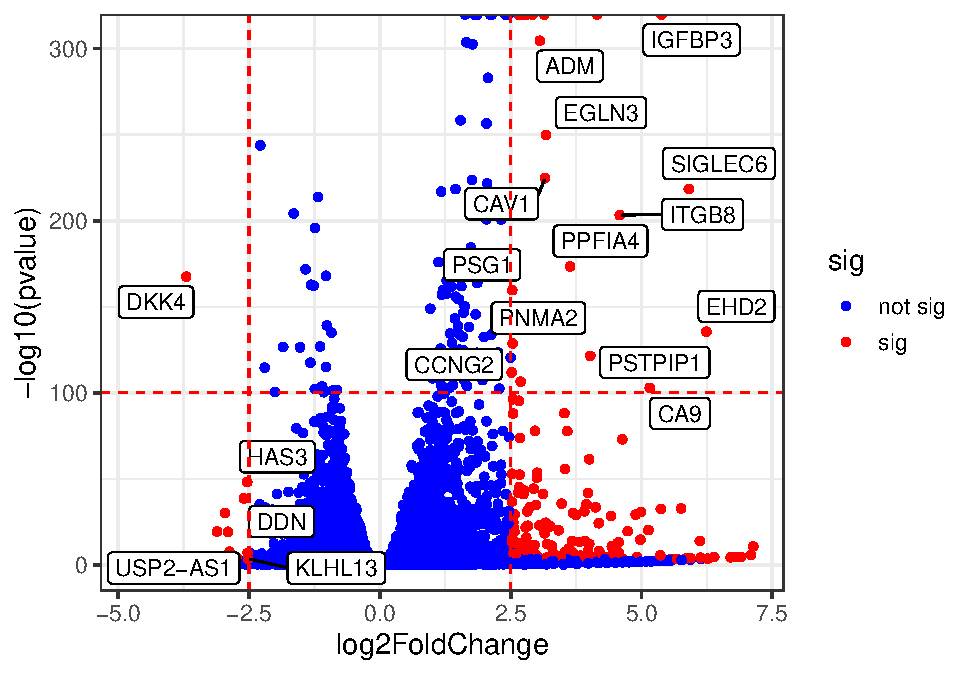
\includegraphics{10_Introduction_to_BioConductor_files/figure-latex/unnamed-chunk-61-1.pdf}

Now, we create the heatmap using the \texttt{Heatmap} function from the \texttt{ComplexHeatmap} package. We specify \texttt{cluster\_columns\ =\ TRUE} to cluster the columns (genes) for better visualization. The \texttt{cell\_fun} parameter is set to our custom function for adding grid lines, and we name the data as ``log2TPM.''

The resulting heatmap will show the median gene expression levels for each gene across different cancer types.

Grid lines will help in distinguishing individual cells within the heatmap so we added them.
This visualization can provide insights into gene expression patterns in various cancer types, which may be useful for further analysis and interpretation.

\hypertarget{step-10-sanity-check-and-scaling-of-gene-expression}{%
\subsection{Step 10: Sanity Check and Scaling of Gene Expression}\label{step-10-sanity-check-and-scaling-of-gene-expression}}

\hypertarget{sanity-check}{%
\subsubsection{Sanity Check}\label{sanity-check}}

Before proceeding with scaling, we will conduct a sanity check of the gene expression heatmap to see if the results make biological sense. For example, we can observe if certain genes are highly expressed in specific cancer types, which could indicate potential biomarkers or interesting biological phenomena.

\begin{Shaded}
\begin{Highlighting}[]
\CommentTok{\# Sanity check}
\NormalTok{sanity\_check\_genes }\OtherTok{\textless{}{-}} \FunctionTok{c}\NormalTok{(}\StringTok{"MSLN"}\NormalTok{, }\StringTok{"FOLH1"}\NormalTok{)}

\CommentTok{\# Extract the rows (genes) corresponding to sanity check genes}
\NormalTok{sanity\_check\_data }\OtherTok{\textless{}{-}}\NormalTok{ tcga\_mat[}\FunctionTok{rownames}\NormalTok{(tcga\_mat) }\SpecialCharTok{\%in\%}\NormalTok{ sanity\_check\_genes, ]}

\CommentTok{\# Print the results}
\FunctionTok{print}\NormalTok{(sanity\_check\_data)}
\end{Highlighting}
\end{Shaded}

\begin{verbatim}
##      TACSTD2 VTCN1 MUC1 NECTIN4 FOLH1 FOLR1 CD276 MSLN CLDN6 ERBB2 MUC16 DLL3
##      CEACAM5 PVR EPCAM PROM1 CD24 EGFR MET TNFRSF10B
\end{verbatim}

We see \texttt{MSLN} is high in \texttt{MESO}, \texttt{FOLH1} is high in prostate cancer (\texttt{PRAD}). We are probably on the right track!

\hypertarget{scaling-the-data}{%
\subsubsection{Scaling the data}\label{scaling-the-data}}

To visualize gene expression in a more comparative manner, we can scale the expression values for each gene across the cancer types. Scaling standardizes the data, making it easier to identify relative expression levels.

\begin{Shaded}
\begin{Highlighting}[]
\CommentTok{\# Scale the expression data}
\NormalTok{scaled\_tcga\_mat }\OtherTok{\textless{}{-}} \FunctionTok{scale}\NormalTok{(tcga\_mat)}

\CommentTok{\# Create a scaled heatmap}
\FunctionTok{Heatmap}\NormalTok{(scaled\_tcga\_mat, }
        \AttributeTok{cluster\_columns =} \ConstantTok{TRUE}\NormalTok{, }
        \AttributeTok{cell\_fun =}\NormalTok{ cell\_fun, }
        \AttributeTok{name =} \StringTok{"scaled}\SpecialCharTok{\textbackslash{}n}\StringTok{log2TPM"}\NormalTok{)}
\end{Highlighting}
\end{Shaded}

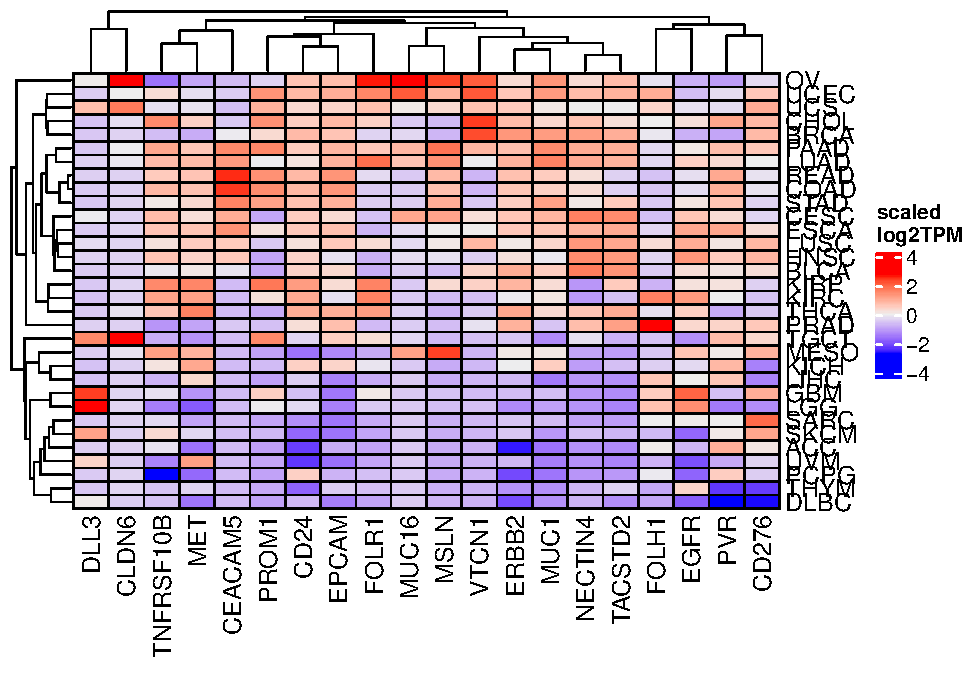
\includegraphics{10_Introduction_to_BioConductor_files/figure-latex/unnamed-chunk-63-1.pdf}

Here, we use the \texttt{scale()} function to standardize the expression values across cancer types for each gene. We then create a new heatmap using the scaled data.

By comparing the original and scaled heatmaps, we can gain insights into how the expression of genes varies relative to each other across different cancer types. This scaling helps us focus on the relative expression patterns rather than the absolute values.

\hypertarget{conclusion-30}{%
\subsection{Conclusion}\label{conclusion-30}}

In this comprehensive example, we have walked through various essential steps for performing gene expression analysis using R, focusing on the analysis of The Cancer Genome Atlas (TCGA) data as an illustrative example. Gene expression analysis is a fundamental component of genomics research, enabling us to uncover insights into the molecular mechanisms underlying complex biological processes, such as cancer.

\hypertarget{section-completed}{%
\section{Section completed}\label{section-completed}}

Congratulations on completing this section!

You've learned crucial genomics data handling and analysis techniques, like using the \texttt{GenomicRanges} package, analyzing CpG islands, converting gene IDs, and creating visualizations with \texttt{ComplexHeatmap}. These skills are vital for bioinformatics, giving you the confidence to navigate genomic data complexities.

Don't hesitate to interact with your peers and instructors in the Q\&A section and comments. Share your experiences, ask questions, and offer support. Your engagement enriches everyone's learning journey.

As you approach the final project, remember that what you've learned is more than just theory---it's practical knowledge you can apply. Use this opportunity to showcase your skills in a real-world scenario. Dive into the challenge with enthusiasm and curiosity.

Good luck!
Let's make this final project a success together!

  \bibliography{book.bib,packages.bib}

\end{document}
